\documentclass[usenames,dvipsnames,Nike,mathserif]{tuberlinbeamer}
\usepackage[english]{babel}  % 'babel' muss geladen werden
\usepackage[utf8]{inputenc}  % optional, aber empfehlenswert
\usepackage[T1]{fontenc}
\usepackage{
	tikz,
	pgfplots,
	pgfplotstable,
	xparse,
	boxedminipage2e,
	amsmath,
	amssymb,
	amsfonts,
	hyperref,
	graphicx,
	soul,
	xcolor,
	color,
	caption,
	subfig,
	booktabs,
	siunitx
	}
\usepackage[skins,theorems]{tcolorbox}
\usepackage[font={small}]{caption}
%Biblography
%\usepackage[natbib=true,style=authoryear,backend=bibtex,useprefix=true]{biblatex}
\usepackage[style=verbose,backend=biber]{biblatex}
\bibliography{references.bib}
%\bibliographystyle{JHEP}
%\addbibresource{other/references}
%colors
\definecolor{color0}{rgb}{0.12156862745098,0.466666666666667,0.705882352941177}
%Mathoperators
\DeclareMathOperator*{\argmin}{\arg\!\min}
\newcommand\inlineeqno{\stepcounter{equation}\ (\theequation)}
%PGF and TIKz
\usepgfplotslibrary{groupplots}
\pgfplotsset{compat=newest}
\usetikzlibrary{
	shapes,
	arrows,
	snakes,
	chains}
\tikzstyle{arrow} = [thick,->,>=stealth]
\tikzstyle{circ} = [circle,minimum size =0.4cm,text centered, draw=black,inner sep = 0pt]
\usetikzlibrary{external,positioning,backgrounds}
\tikzexternalize[prefix=Figures/]
% Die ueblichen Angaben
\title{Model Order Reduction of Rarefied Gases Using Neural Networks}
\subtitle{}
\author[Zachary Schellin]{Zachary Schellin}
\institute{Institut f\"ur Numerische Fluiddynamik}

% Eigenes Logo einfuegen:
\renewcommand{\pathtomylogo}{csm_cfd_logo_invers_ohne_schrift_blauer_hintergrund_3fa262aacf.png}
%COntext after every Section
\AtBeginSection[]
{
	\begin{frame}
		\frametitle{Table of Contents}
		\tableofcontents[currentsection]
	\end{frame}
}
\begin{document}

\begin{frame}
\maketitle
\end{frame}


\begin{frame}[fragile]{Outline}
\tableofcontents
\end{frame}
\section{Introduction}
%%%%%%%%%%%%%%%%%%%%%%%%%%%%%%%%%%%%%%%%%%%%%%%%%%%%%%%%%%%%%%%%%%%%%%%%
\section{The BGK-Model}
\begin{frame}[fragile]{Governing equations}
\begin{columns}
	\begin{column}{.5\textwidth}
		 \onslide<1->{\emph{Boltzmann equation with the BGK operator}
		\begin{equation}
			\tcbhighmath[
			size=title,title=transport,boxrule=0.4pt,colframe=blue,drop fuzzy shadow=green]{\partial_t f + v \partial_x f} =
			 \tcbhighmath[
			 size=title,title=collisions,boxrule=0.4pt,colframe=red,drop fuzzy shadow=red]{\frac{1}{\tau} (M_f - f)}
		\end{equation}}
	\end{column}
	\begin{column}{.5\textwidth}
		\onslide<2->{\emph{Equilibrium solution}: Maxwellian distribution $\boldsymbol{M_f}$
		\vspace{1.5em}
		\begin{equation}
			M_f = \frac{\rho(x,t)}{(2\pi R T(x,t))^{\frac{3}{2}}}\exp(-\frac{(v - u(x,t))^2}{2 R T(x,t)}) 
		\end{equation}}
	\end{column}
\end{columns}\vspace{2em}
\begin{columns}
	\begin{column}{.5\textwidth}
		\onslide<3->{\emph{Duration to evolve into equilibrium}: relaxation time $\boldsymbol{\tau}$
		\begin{equation}
			\tau^{-1} = \frac{\rho(x,t)T^{1-\nu}(x,t)}{Kn}
		\end{equation}}
	\end{column}
	\begin{column}{.5\textwidth}
		\onslide<4->{\emph{Rarefaction level}: Knudsen number $\boldsymbol{Kn}$
		\vspace{1em}
		\begin{equation}
			Kn = \frac{\lambda}{l}
		\end{equation}}
	\end{column}
\end{columns}
\footcite{PhysRev.94.511}
\end{frame}

\begin{frame}[fragile]{Knudsen number}
	\onslide<1->{\begin{center}
			\begin{figure}
			\centering
			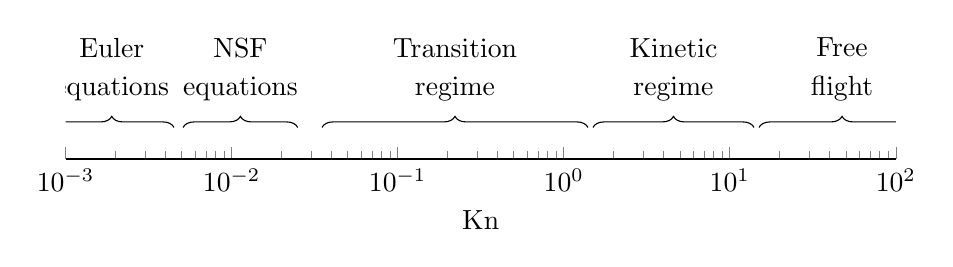
\begin{tikzpicture}
\begin{axis}[
    y=5cm,            % y unit vector
    hide y axis,        % hide the y axis
    xmode = log,        % logarithmic x axis
    axis x line*=bottom,% only show the bottom x axis line, without an arrow tip
    xmin=1e-3, xmax=1e2,% range for the x axis
    xlabel = Kn,
    width=\textwidth
]
\addplot [draw=none] coordinates {(0.001,0.9)};
\draw [decorate,decoration={brace,amplitude=4pt}] (axis cs:0.0008,.8) -- (axis cs: 0.0045,.8) node[rectangle split,rectangle split parts=2,midway,above=6pt] {Euler \nodepart{second} equations};
\draw [decorate,decoration={brace,amplitude=4pt}] (axis cs:0.0051,.8) -- (axis cs: 0.025,.8) node[rectangle split,rectangle split parts=2,midway,above=6pt] {NSF \nodepart{second} equations};
\draw [decorate,decoration={brace,amplitude=4pt}] (axis cs:0.035,.8) -- (axis cs: 1.4,.8) node[rectangle split,rectangle split parts=2,midway,above=6pt] {Transition  \nodepart{second} regime};
\draw [decorate,decoration={brace,amplitude=4pt}] (axis cs:1.5,.8) -- (axis cs: 14,.8) node[rectangle split,rectangle split parts=2,midway,above=6pt] {Kinetic  \nodepart{second} regime};
\draw [decorate,decoration={brace,amplitude=4pt}] (axis cs:15,.8) -- (axis cs: 150,.8) node[rectangle split,rectangle split parts=2,midway,above=6pt] {Free  \nodepart{second} flight};
%\draw [<->] (axis cs:0.001,-.8) -- (axis cs: 0.006,-.8) node[midway,fill=white] {Equilibrium};
\end{axis}
\end{tikzpicture}
			\caption{Partitioning of $Kn$ into levels of rarefaction.}
			\label{Fig:ExpKN}
			\footfullcite{NumaKUL}
		\end{figure}}
	\end{center}
	\onslide<2->{\begin{itemize}
		\item Solution is $\mathbf{f(x,v,t)}$ in 1D and $\mathbf{f(x,y,v_x,v_y,t)}$ in 2D and $\mathbf{f(x,y,z,v_x,v_y,v_z,t)}$ in 3D 
\end{itemize}}
\vspace{1em}
\end{frame}

\begin{frame}[fragile]{Discretization in space and velocity space in 1D}
	\begin{itemize}
		\item<1-> \emph{Space and time discretization}:
		 $x_j = j\Delta x$ and $j\in \mathbb{Z}$, $v_k = k\Delta v$ and $k\in \mathbb{Z}$, $t^i=i\Delta t$ and $t\in \mathbb{N}$,
		\item<2-> \emph{Leads to:} set of ODE's in time 
			\begin{equation}
			\partial_t f_{j,k} = -(v_k)_1D_x f|_{j,k}(t) + \frac{1}{\tau}({M_f}_{j,k}(t) - f_{j,k}(t))\mathrm{.}
			\end{equation}
		\item<3-> \emph{$\mathbf{KJ}$ first-order differential equations}:\\
		$K$ gridpoints in space \& $J$ number of gridpoints in velocity space
		\item<4-> \emph{3D}:\\ $K^3J^3$ first-order differential equations
		\item<5-> \emph{Evaluation requires}: the moments of $f$.
	\end{itemize}
\end{frame}

\begin{frame}[fragile]{Moments/ Expected values of $f$}
	\begin{columns}
		\begin{column}{.5\textwidth}
			\onslide<1->{\emph{Question}: How do we get the moments of $f$?}
				\begin{itemize}
				\item<2-> Collision invariants $\Phi(v)=[1,v,\frac{1}{2}v^2]$
				\item<3-> The first moment/ \emph{Density} is
				\begin{equation}
					\rho(x,t) = \int\! f \,\mathrm{d}v \,,
				\end{equation}
				\item<4-> the second moment/ \emph{Momentum} is
				\begin{equation}
					\rho(x,t) u(x,t) = \int\! v f \,\mathrm{d}v \,,
				\end{equation}
				\item<5-> the third moment/ \emph{Energy} is
				\begin{equation}
					E(x,t) = \int\! \frac{1}{2}v^2 f  \,\mathrm{d}v \,.
				\end{equation}
			\end{itemize}
		\end{column}
		\begin{column}{.5\textwidth}
			\begin{center}
				\begin{figure}
					% This file was created by tikzplotlib v0.9.6.
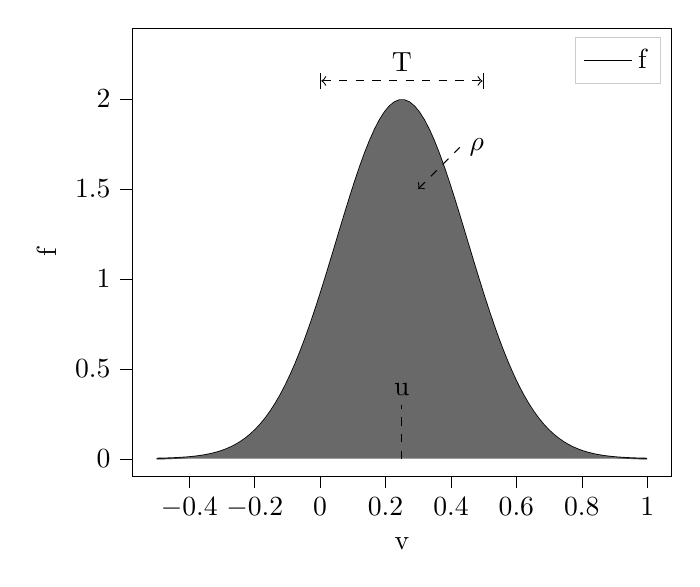
\begin{tikzpicture}

\begin{axis}[
legend cell align={left},
legend style={fill opacity=0.8, draw opacity=1, text opacity=1, draw=white!80!black},
tick align=outside,
tick pos=left,
x grid style={white!69.0196078431373!black},
xlabel={v},
xmin=-0.575, xmax=1.075,
xtick style={color=black},
y grid style={white!69.0196078431373!black},
ylabel={f},
ymin=-0.0978129180007683, ymax=2.39285680307655,
ytick style={color=black}
]

\addplot [semithick, black]
table {%
	-0.5 0.00176297841183723
	-0.484848484848485 0.00233549990938288
	-0.46969696969697 0.00307623995021814
	-0.454545454545455 0.0040287289903483
	-0.439393939393939 0.00524594088238899
	-0.424242424242424 0.00679182087082491
	-0.409090909090909 0.00874292085377632
	-0.393939393939394 0.0111901101946249
	-0.378787878787879 0.0142403174963827
	-0.363636363636364 0.018018244420721
	-0.348484848484849 0.0226679772544878
	-0.333333333333333 0.0283544060972295
	-0.318181818181818 0.0352643460570684
	-0.303030303030303 0.0436072406856785
	-0.287878787878788 0.0536153162176469
	-0.272727272727273 0.0655430473059348
	-0.257575757575758 0.0796657922473926
	-0.242424242424242 0.0962774595613305
	-0.227272727272727 0.115687079522804
	-0.212121212121212 0.138214174964358
	-0.196969696969697 0.164182856129127
	-0.181818181818182 0.193914604924168
	-0.166666666666667 0.227719764364528
	-0.151515151515151 0.265887808434693
	-0.136363636363636 0.308676534413689
	-0.121212121212121 0.356300391543538
	-0.106060606060606 0.408918233661475
	-0.0909090909090909 0.466620855301653
	-0.0757575757575757 0.529418736525693
	-0.0606060606060606 0.597230476778283
	-0.0454545454545454 0.669872437749538
	-0.0303030303030303 0.747050135179608
	-0.0151515151515151 0.828351915965591
	0 0.91324542694511
	0.0151515151515151 1.00107732368077
	0.0303030303030303 1.09107658129022
	0.0454545454545454 1.18236165636822
	0.0606060606060607 1.2739516126026
	0.0757575757575758 1.36478116780159
	0.0909090909090909 1.45371945330681
	0.106060606060606 1.53959210603912
	0.121212121212121 1.62120614747867
	0.136363636363636 1.69737695187443
	0.151515151515151 1.76695647690227
	0.166666666666667 1.82886183207001
	0.181818181818182 1.88210320029322
	0.196969696969697 1.92581011126961
	0.212121212121212 1.95925509432898
	0.227272727272727 1.98187381354832
	0.242424242424242 1.99328090666395
	0.257575757575758 1.99328090666395
	0.272727272727273 1.98187381354832
	0.287878787878788 1.95925509432898
	0.303030303030303 1.92581011126961
	0.318181818181818 1.88210320029322
	0.333333333333333 1.82886183207001
	0.348484848484849 1.76695647690227
	0.363636363636364 1.69737695187443
	0.378787878787879 1.62120614747867
	0.393939393939394 1.53959210603912
	0.409090909090909 1.45371945330681
	0.424242424242424 1.36478116780159
	0.439393939393939 1.2739516126026
	0.454545454545455 1.18236165636822
	0.46969696969697 1.09107658129022
	0.484848484848485 1.00107732368077
	0.5 0.91324542694511
	0.515151515151515 0.828351915965591
	0.53030303030303 0.747050135179608
	0.545454545454545 0.669872437749538
	0.560606060606061 0.597230476778283
	0.575757575757576 0.529418736525694
	0.590909090909091 0.466620855301653
	0.606060606060606 0.408918233661474
	0.621212121212121 0.356300391543538
	0.636363636363636 0.308676534413689
	0.651515151515152 0.265887808434693
	0.666666666666667 0.227719764364528
	0.681818181818182 0.193914604924168
	0.696969696969697 0.164182856129127
	0.712121212121212 0.138214174964358
	0.727272727272727 0.115687079522804
	0.742424242424242 0.0962774595613305
	0.757575757575758 0.0796657922473926
	0.772727272727273 0.0655430473059348
	0.787878787878788 0.0536153162176469
	0.803030303030303 0.0436072406856785
	0.818181818181818 0.0352643460570684
	0.833333333333333 0.0283544060972294
	0.848484848484849 0.0226679772544878
	0.863636363636364 0.018018244420721
	0.878787878787879 0.0142403174963826
	0.893939393939394 0.0111901101946249
	0.909090909090909 0.00874292085377631
	0.924242424242424 0.00679182087082491
	0.939393939393939 0.00524594088238899
	0.954545454545455 0.0040287289903483
	0.96969696969697 0.00307623995021814
	0.984848484848485 0.00233549990938288
	1 0.00176297841183723
};
\addlegendentry{f}

\path [draw=none, fill=white!41.1764705882353!black]
(axis cs:-0.5,0.00176297841183723)
--(axis cs:-0.484848484848485,0.00233549990938288)
--(axis cs:-0.46969696969697,0.00307623995021814)
--(axis cs:-0.454545454545455,0.0040287289903483)
--(axis cs:-0.439393939393939,0.00524594088238899)
--(axis cs:-0.424242424242424,0.00679182087082491)
--(axis cs:-0.409090909090909,0.00874292085377632)
--(axis cs:-0.393939393939394,0.0111901101946249)
--(axis cs:-0.378787878787879,0.0142403174963827)
--(axis cs:-0.363636363636364,0.018018244420721)
--(axis cs:-0.348484848484849,0.0226679772544878)
--(axis cs:-0.333333333333333,0.0283544060972295)
--(axis cs:-0.318181818181818,0.0352643460570684)
--(axis cs:-0.303030303030303,0.0436072406856785)
--(axis cs:-0.287878787878788,0.0536153162176469)
--(axis cs:-0.272727272727273,0.0655430473059348)
--(axis cs:-0.257575757575758,0.0796657922473926)
--(axis cs:-0.242424242424242,0.0962774595613305)
--(axis cs:-0.227272727272727,0.115687079522804)
--(axis cs:-0.212121212121212,0.138214174964358)
--(axis cs:-0.196969696969697,0.164182856129127)
--(axis cs:-0.181818181818182,0.193914604924168)
--(axis cs:-0.166666666666667,0.227719764364528)
--(axis cs:-0.151515151515151,0.265887808434693)
--(axis cs:-0.136363636363636,0.308676534413689)
--(axis cs:-0.121212121212121,0.356300391543538)
--(axis cs:-0.106060606060606,0.408918233661475)
--(axis cs:-0.0909090909090909,0.466620855301653)
--(axis cs:-0.0757575757575757,0.529418736525693)
--(axis cs:-0.0606060606060606,0.597230476778283)
--(axis cs:-0.0454545454545454,0.669872437749538)
--(axis cs:-0.0303030303030303,0.747050135179608)
--(axis cs:-0.0151515151515151,0.828351915965591)
--(axis cs:0,0.91324542694511)
--(axis cs:0.0151515151515151,1.00107732368077)
--(axis cs:0.0303030303030303,1.09107658129022)
--(axis cs:0.0454545454545454,1.18236165636822)
--(axis cs:0.0606060606060607,1.2739516126026)
--(axis cs:0.0757575757575758,1.36478116780159)
--(axis cs:0.0909090909090909,1.45371945330681)
--(axis cs:0.106060606060606,1.53959210603912)
--(axis cs:0.121212121212121,1.62120614747867)
--(axis cs:0.136363636363636,1.69737695187443)
--(axis cs:0.151515151515151,1.76695647690227)
--(axis cs:0.166666666666667,1.82886183207001)
--(axis cs:0.181818181818182,1.88210320029322)
--(axis cs:0.196969696969697,1.92581011126961)
--(axis cs:0.212121212121212,1.95925509432898)
--(axis cs:0.227272727272727,1.98187381354832)
--(axis cs:0.242424242424242,1.99328090666395)
--(axis cs:0.257575757575758,1.99328090666395)
--(axis cs:0.272727272727273,1.98187381354832)
--(axis cs:0.287878787878788,1.95925509432898)
--(axis cs:0.303030303030303,1.92581011126961)
--(axis cs:0.318181818181818,1.88210320029322)
--(axis cs:0.333333333333333,1.82886183207001)
--(axis cs:0.348484848484849,1.76695647690227)
--(axis cs:0.363636363636364,1.69737695187443)
--(axis cs:0.378787878787879,1.62120614747867)
--(axis cs:0.393939393939394,1.53959210603912)
--(axis cs:0.409090909090909,1.45371945330681)
--(axis cs:0.424242424242424,1.36478116780159)
--(axis cs:0.439393939393939,1.2739516126026)
--(axis cs:0.454545454545455,1.18236165636822)
--(axis cs:0.46969696969697,1.09107658129022)
--(axis cs:0.484848484848485,1.00107732368077)
--(axis cs:0.5,0.91324542694511)
--(axis cs:0.515151515151515,0.828351915965591)
--(axis cs:0.53030303030303,0.747050135179608)
--(axis cs:0.545454545454545,0.669872437749538)
--(axis cs:0.560606060606061,0.597230476778283)
--(axis cs:0.575757575757576,0.529418736525694)
--(axis cs:0.590909090909091,0.466620855301653)
--(axis cs:0.606060606060606,0.408918233661474)
--(axis cs:0.621212121212121,0.356300391543538)
--(axis cs:0.636363636363636,0.308676534413689)
--(axis cs:0.651515151515152,0.265887808434693)
--(axis cs:0.666666666666667,0.227719764364528)
--(axis cs:0.681818181818182,0.193914604924168)
--(axis cs:0.696969696969697,0.164182856129127)
--(axis cs:0.712121212121212,0.138214174964358)
--(axis cs:0.727272727272727,0.115687079522804)
--(axis cs:0.742424242424242,0.0962774595613305)
--(axis cs:0.757575757575758,0.0796657922473926)
--(axis cs:0.772727272727273,0.0655430473059348)
--(axis cs:0.787878787878788,0.0536153162176469)
--(axis cs:0.803030303030303,0.0436072406856785)
--(axis cs:0.818181818181818,0.0352643460570684)
--(axis cs:0.833333333333333,0.0283544060972294)
--(axis cs:0.848484848484849,0.0226679772544878)
--(axis cs:0.863636363636364,0.018018244420721)
--(axis cs:0.878787878787879,0.0142403174963826)
--(axis cs:0.893939393939394,0.0111901101946249)
--(axis cs:0.909090909090909,0.00874292085377631)
--(axis cs:0.924242424242424,0.00679182087082491)
--(axis cs:0.939393939393939,0.00524594088238899)
--(axis cs:0.954545454545455,0.0040287289903483)
--(axis cs:0.96969696969697,0.00307623995021814)
--(axis cs:0.984848484848485,0.00233549990938288)
--(axis cs:1,0.00176297841183723)
--cycle;
\addlegendimage{area legend, draw=none, fill=white!41.1764705882353!black}




\draw [dashed,|<->|] (axis cs:0,2.1) -- (axis cs:0.5,2.1);
\draw [] (axis cs:0.25,2.1) node[above] {T};
\draw [dashed] (axis cs:0.25,0)--(axis cs:0.25,0.3);
\draw [] (axis cs:0.25,0.3) node[above] {u};
\draw [dashed,<-] (axis cs:0.3,1.5)-- +(15pt,15pt) node[right] {\(\rho\)};
\end{axis}
\end{tikzpicture}

					\caption{Illustration of the linkage between \(f\) and the moments of \(f\).}
				\end{figure}
			\end{center}
		\end{column}
	\end{columns}
\end{frame}

\section{Sod's shock tube}
%%%%%%%%%%%%%%%%%%%%%%%%%%%%%%%%%%%%%%%%%%%%%%%%%%%%%%%%%%%%%%%
\begin{frame}[fragile]{Sod's shock tube}
	\begin{columns}
		\begin{column}{.5\textwidth}
				\begin{figure}
					\only<1>{\begin{tikzpicture}
	\draw (1,0) rectangle +(2,1)
\end{tikzpicture}}
					\only<1>{\caption{Problem setup of Sod's shock tube for the BGK model in 1D at $t=0s$.}}
					\only<2>{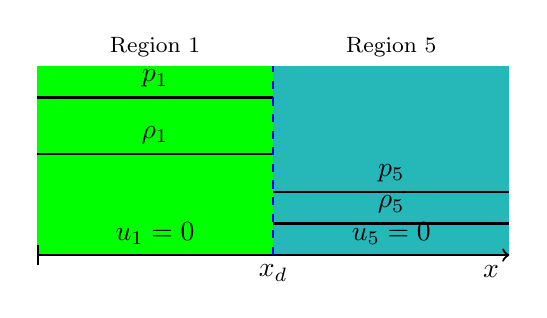
\begin{tikzpicture}[scale=0.8]
	\draw[draw=none,fill=BlueGreen] (3.75,0.0) rectangle ++(3.75,3);
	\draw[draw=none,fill=green] (0.0,0.0) rectangle ++(3.75,3);
		%ground nodes
	\node [] at (0,0) (a0) {};
	\node [] at (3.75,0) (a3) {};
	\node [] at (7.5,0) (a6) {};
	\node [on grid,below = 1.5ex of a3] (xd) {$x_d$};
		%level 1 nodes
	\node [] at (0,1.6) (f0) {};
	\node [] at (3.75,1.6) (f1) {};
	\node [] at (7.5,0.5) (b6) {};
	
		%level 2 nodes
	\node [] at (0,2.5) (h0) {};
	\node [] at (3.75,2.5) (h1) {};
	\node [] at (3.75,0.5) (b3) {};
	\node [] at (7.5,1) (d6) {};
	\node [] at (3.75,1) (d3) {};	
		%top nodes
	\node [] at (0,3) (i0) {};
	\node [] at (3.75,3) (i3) {};
	\node [] at (7.5,3) (i6) {};
	
	\draw[|-,thick] (a0.center) -- (a3.center) node [midway,above] {$u_1=0$};
	\draw[thick] (f0.center) -- (f1.center) node [midway,above] {$\rho_1$};
	\draw[thick] (h0.center) -- (h1.center) node [midway,above] {$p_1$};
	
	\draw[->,thick] (a3.center) -- (a6.center) node [midway,above] { $u_5=0$} node [below left] {$x$};
	\draw[thick] (b3.center) -- (b6.center) node [midway,above] {$\rho_5$};
	\draw[thick] (d3.center) -- (d6.center) node [midway,above] {$p_5$};
	\draw[thick,dashed,blue] (a3.center) -- (i3.center) {};
	\path[] (i0.center) -- (i3.center) node [midway,above] {\footnotesize Region 1};
	\path[] (i3.center) -- (i6.center) node [midway,above] {\footnotesize Region 5};
	
	
	
\end{tikzpicture}}
					\only<2>{\caption{Problem setup of Sod's shock tube for the BGK model in 1D at $t=0s$.}}
					\onslide<3->{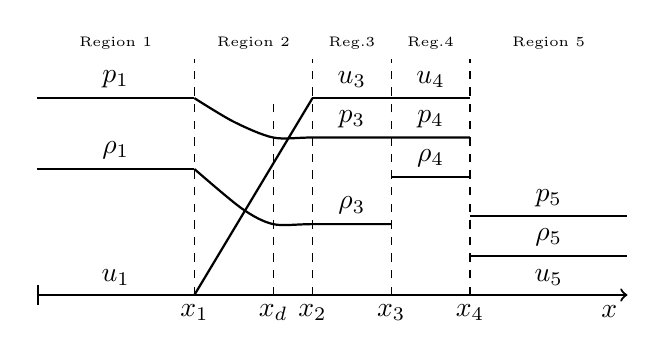
\begin{tikzpicture}
	%ground nodes
	\node [] at (0,0) (a0) {};
	\node [] at (2,0) (a1) {};
	\node [] at (3,0) (a2) {};
	\node [] at (3.5,0) (a3) {};
	\node [] at (4.5,0) (a4) {};
	\node [] at (5.5,0) (a5) {};
	\node [] at (7.5,0) (a6) {};
	\node [on grid,below = 1.5ex of a2] (xd) {$x_d$};
	\node [on grid,below = 1.5ex of a1] (x1) {$x_1$};
	\node [on grid,below = 1.5ex of a3] (x2) {$x_2$};
	\node [on grid,below = 1.5ex of a4] (x3) {$x_3$};
	\node [on grid,below = 1.5ex of a5] (x4) {$x_4$};
	%level 1 nodes
	\node [] at (7.5,0.5) (b6) {};
	\node [] at (5.5,0.5) (b5) {};
	%level 2 nodes
	\node [] at (3,.9) (c2) {};
	\node [] at (3.5,.9) (c3) {};
	\node [] at (4.5,.9) (c4) {};
	%level 3 nodes
	\node [] at (7.5,1) (d6) {};
	\node [] at (5.5,1) (d5) {};
	%level 4 nodes
	\node [] at (4.5,1.5) (e4) {};
	\node [] at (5.5,1.5) (e5) {};
	%level 5 nodes
	\node [] at (0,1.6) (f0) {};
	\node [] at (2,1.6) (f1) {};
	%level 6 nodes
	\node [] at (3,2) (g2) {};
	\node [] at (3.5,2) (g3) {};
	\node [] at (4.5,2) (g4) {};
	\node [] at (5.5,2) (g5) {};
	\node [] at (7.5,2) (g6) {};
	%level 7 nodes
	\node [] at (0,2.5) (h0) {};
	\node [] at (2,2.5) (h1) {};
	\node [] at (3,2.5) (h2) {};
	\node [] at (3.5,2.5) (h3) {};
	\node [] at (4.5,2.5) (h4) {};
	\node [] at (5.5,2.5) (h5) {};
	%top nodes
	\node [] at (0,3) (i0) {};
	\node [] at (2,3) (i1) {};
	\node [] at (3,3) (i2) {};
	\node [] at (3.5,3) (i3) {};
	\node [] at (4.5,3) (i4) {};
	\node [] at (5.5,3) (i5) {};
	\node [] at (7.5,3) (i6) {};
	%draw and bottom edge
	\draw [|->,thick] (a0.center) -- (a6.center) node [below left] {$x$};
	\path [] (a0.center) -- (a1.center) node [midway,above] {$u_1$};
	\path [] (a5.center) -- (a6.center) node [midway,above] { $u_5$};
	%draw top descriptors
	\path[] (i0.center) -- (i1.center) node [midway,above] {\tiny Region 1};
	\path[] (i1.center) -- (i3.center) node [midway,above] {\tiny Region 2};
	\path[] (i3.center) -- (i4.center) node [midway,above] {\tiny Reg.3};
	\path[] (i4.center) -- (i5.center) node [midway,above] {\tiny Reg.4};
	\path[] (i5.center) -- (i6.center) node [midway,above] {\tiny Region 5};
	%draw level 1
	\draw[thick] (b5.center) -- (b6.center) {};
	\path[] (b5.center) -- (b6.center) node [midway,above] {$\rho_5$};
	%draw level 3
	\path[] (c3.center) -- (c4.center) node [midway,above] {$\rho_3$};
	%draw level 4
	\draw[thick] (d5.center) -- (d6.center) {};
	\path[] (d5.center) -- (d6.center) node [midway,above] {$p_5$};
	%draw level 5
	\draw[thick] (e4.center) -- (e5.center) {};
	\path[] (e4.center) -- (e5.center) node [midway,above] {$\rho_4$};
	\draw[thick] plot [smooth] coordinates {(f1)(2.6,1.1)(c2)(c3)(c4)};
	\draw[thick] (f0.center) -- (f1.center) node [midway,above] {$\rho_1$};
	%draw level 6
	\path[] (g3.center) -- (g4.center) node [midway,above] {$p_3$};
	\path[] (g4.center) -- (g5.center) node [midway,above] {$p_4$};
	\draw[thick] plot [smooth] coordinates {(h1)(2.5,2.2)(g2)(g3)(g4)(g5)};
	\draw[thick] (h3.center) -- (a1.center) {};

	\draw[thick] (h0.center) -- (h1.center) node [midway,above] {$p_1$};
	\draw[thick] (h3.center) -- (h4.center) node [midway,above] {$u_3$};
	\draw[thick] (h4.center) -- (h5.center) node [midway,above] {$u_4$};
	%draw vertical lines
	\draw[dashed] (a1.center) -- (i1.center) {};
	\draw[dashed] (a2.center) -- (h2.center) {};
	\draw[dashed] (a3.center) -- (i3.center) {};
	\draw[dashed] (a4.center) -- (i4.center) {};
	\draw[dashed] (a5.center) -- (i5.center) {};

\end{tikzpicture}}
					\onslide<3->{\caption{Problem setup of Sod's shock tube for the BGK model in 1D at $t>0s$.}}
			\end{figure}
		\end{column}
		\begin{column}{.5\textwidth}
			\vspace{-1em}
				\begin{itemize}
					\item \emph{Test case} for numerical schemes solving
					\item \emph{non-linear hyperbolic conservation laws} in gas dynamics (Gary A. Sod in 1978)
					\item \emph{Idea}:
					\begin{itemize}
						\item Solve problem analytically (Rankine-Hugoniot jump conditions)
						\item Solve problem numerically
						\item Compare results expecially \emph{resolution of discontinuities}
				   \onslide<3->{\begin{itemize}
								\item<4-> \colorbox{green}{$\mathbf{x_1}$ head of rarefaction wave}
								\item<4-> \colorbox{green}{$\mathbf{x_2}$ tail of rarefaction wave}
								\item<5-> \colorbox{yellow}{$\mathbf{x_3}$ contact discontinuity}
								\item<6-> \colorbox{BlueGreen}{$\mathbf{x_4}$ position of shockwave}
							\end{itemize}}
					\end{itemize}
				\end{itemize}
		\end{column}
	\end{columns}
\end{frame}
\begin{frame}[fragile]{Two Case Studies}
	\begin{columns}
		\begin{column}{.5\textwidth}
			\begin{figure}
				% This file was created by tikzplotlib v0.9.6.
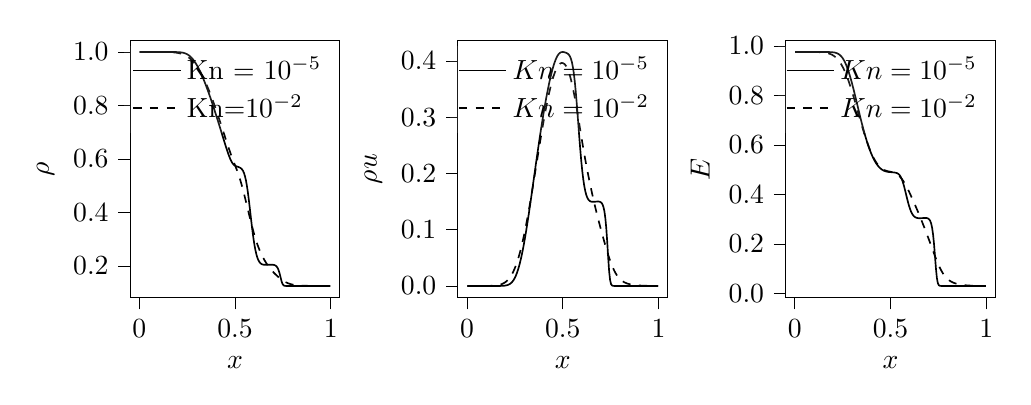
\begin{tikzpicture}

\begin{groupplot}[group style={group size=3 by 1,horizontal sep=1.5cm}]
\nextgroupplot[
legend cell align={left},
legend style={fill opacity=0.1, draw opacity=1, text opacity=1, draw=none},
tick align=outside,
tick pos=left,
x grid style={white!69.0196078431373!black},
xlabel={\(x\)},
xmin=-0.04725, xmax=1.04725,
xtick style={color=black},
y grid style={white!69.0196078431373!black},
ylabel={\(\rho\)},
ymin=0.0812472272613489, ymax=1.04375013203517,
ytick style={color=black},
ytick={0,0.2,0.4,0.6,0.8,1,1.2},
yticklabels={0.0,0.2,0.4,0.6,0.8,1.0,1.2},
width=.35\textwidth,
height=.4\textwidth
]
\addplot [semithick, black]
table {%
0.0025 0.999999999999998
0.0075 0.999999999999989
0.0125 0.999999999999973
0.0175 0.999999999999938
0.0225 0.999999999999854
0.0275 0.999999999999657
0.0325 0.999999999999225
0.0375 0.999999999998307
0.0425 0.999999999996346
0.0475 0.999999999992153
0.0525 0.999999999983302
0.0575 0.999999999964812
0.0625 0.999999999926618
0.0675 0.999999999848593
0.0725 0.999999999691032
0.0775 0.999999999376523
0.0825 0.999999998755951
0.0875 0.999999997545765
0.0925 0.999999995213722
0.0975 0.999999990773699
0.1025 0.999999982422727
0.1075 0.999999966908873
0.1125 0.999999938447061
0.1175 0.999999886889466
0.1225 0.999999794688685
0.1275 0.999999631942622
0.1325 0.999999348451367
0.1375 0.999998861215854
0.1425 0.99999803513588
0.1475 0.999996653797842
0.1525 0.999994376182765
0.1575 0.999990673914891
0.1625 0.999984742419316
0.1675 0.999975378267931
0.1725 0.999960814384862
0.1775 0.999938505100111
0.1825 0.999904854832319
0.1875 0.999854888023955
0.1925 0.99978186432473
0.1975 0.999676852094109
0.2025 0.9995282847065
0.2075 0.999321536763255
0.2125 0.999038569143143
0.2175 0.998657700112069
0.2225 0.998153561405535
0.2275 0.997497290690344
0.2325 0.996656993873317
0.2375 0.99559848331206
0.2425 0.994286264568487
0.2475 0.992684710498992
0.2525 0.990759333664029
0.2575 0.988478051967666
0.2625 0.98581234145918
0.2675 0.982738184425117
0.2725 0.979236747133095
0.2775 0.975294754490673
0.2825 0.970904562368228
0.2875 0.966063957098391
0.2925 0.960775732208377
0.2975 0.955047103436866
0.3025 0.948889025126006
0.3075 0.942315466055067
0.3125 0.935342693163985
0.3175 0.927988599833952
0.3225 0.920272103437352
0.3275 0.912212626120219
0.3325 0.903829663999579
0.3375 0.895142443413195
0.3425 0.886169658461554
0.3475 0.876929281542178
0.3525 0.867438437521144
0.3575 0.857713332238945
0.3625 0.847769226883468
0.3675 0.837620451126894
0.3725 0.827280449648232
0.3775 0.816761858656435
0.3825 0.806076611284112
0.3875 0.795236073302906
0.3925 0.784251213671778
0.3975 0.773132818216759
0.4025 0.761891759626233
0.4075 0.750539343464475
0.4125 0.739087758804205
0.4175 0.727550674370907
0.4225 0.715944038086624
0.4275 0.704287161112698
0.4325 0.692604198229712
0.4375 0.680926174533778
0.4425 0.669293749303168
0.4475 0.657760935139416
0.4525 0.646399961099968
0.4575 0.635307285171405
0.4625 0.62461023214634
0.4675 0.614472547467368
0.4725 0.605094999885858
0.4775 0.596704255186181
0.4825 0.58952161507939
0.4875 0.583707951716951
0.4925 0.579297599755217
0.4975 0.576156316434373
0.5025 0.574000969056694
0.5075 0.572480179189811
0.5125 0.571264203656635
0.5175 0.570086382765471
0.5225 0.568721460109119
0.5275 0.566925165174661
0.5325 0.564365792996614
0.5375 0.560570509046267
0.5425 0.554906055797055
0.5475 0.546613499580239
0.5525 0.534908971753206
0.5575 0.51914228036301
0.5625 0.498978621789052
0.5675 0.474548680779275
0.5725 0.446512149382244
0.5775 0.416003356002158
0.5825 0.384466862363659
0.5875 0.35342828965285
0.5925 0.324264603478363
0.5975 0.298031575214768
0.6025 0.275379774683857
0.6075 0.25655829783077
0.6125 0.241481617940157
0.6175 0.229826469375018
0.6225 0.221130574377751
0.6275 0.214876145355647
0.6325 0.210551637309679
0.6375 0.207691967900792
0.6425 0.205900479181207
0.6475 0.204856774754392
0.6525 0.204314508374631
0.6575 0.204092813817174
0.6625 0.204064484192581
0.6675 0.204143252251004
0.6725 0.204271660594381
0.6775 0.204410149561804
0.6825 0.204527209819603
0.6875 0.2045897518297
0.6925 0.204552165643129
0.6975 0.204341777937618
0.7025 0.203837534924661
0.7075 0.202838126194388
0.7125 0.201017076265398
0.7175 0.197870634170907
0.7225 0.192691647141719
0.7275 0.184667360813301
0.7325 0.173289806057922
0.7375 0.159203831239715
0.7425 0.144954929560638
0.7475 0.134090936270534
0.7525 0.128237751279186
0.7575 0.125970039515887
0.7625 0.125265822009891
0.7675 0.125069122324036
0.7725 0.125016332608434
0.7775 0.125002354962472
0.7825 0.12499867180924
0.7875 0.124997703549099
0.7925 0.124997449439354
0.7975 0.124997382859364
0.8025 0.12499736544419
0.8075 0.124997360897239
0.8125 0.124997359712403
0.8175 0.124997359404317
0.8225 0.124997359324391
0.8275 0.124997359303707
0.8325 0.124997359298369
0.8375 0.124997359296995
0.8425 0.124997359296643
0.8475 0.124997359296553
0.8525 0.12499735929653
0.8575 0.124997359296525
0.8625 0.124997359296523
0.8675 0.124997359296523
0.8725 0.124997359296523
0.8775 0.124997359296523
0.8825 0.124997359296523
0.8875 0.124997359296523
0.8925 0.124997359296523
0.8975 0.124997359296523
0.9025 0.124997359296523
0.9075 0.124997359296523
0.9125 0.124997359296523
0.9175 0.124997359296523
0.9225 0.124997359296523
0.9275 0.124997359296523
0.9325 0.124997359296523
0.9375 0.124997359296523
0.9425 0.124997359296523
0.9475 0.124997359296523
0.9525 0.124997359296523
0.9575 0.124997359296523
0.9625 0.124997359296523
0.9675 0.124997359296523
0.9725 0.124997359296523
0.9775 0.124997359296523
0.9825 0.124997359296523
0.9875 0.124997359296523
0.9925 0.124997359296523
0.9975 0.124997359296523
};
\addlegendentry{Kn = \(10^{-5}\)}
\addplot [semithick, black, dashed]
table {%
0.0025 0.99999981316608
0.0075 0.99999975421908
0.0125 0.999999680296827
0.0175 0.999999584015259
0.0225 0.999999457570282
0.0275 0.999999291316442
0.0325 0.999999072816931
0.0375 0.999998785865599
0.0425 0.999998409307099
0.0475 0.999997915549681
0.0525 0.999997268671227
0.0575 0.999996422006429
0.0625 0.999995315081933
0.0675 0.999993869739663
0.0725 0.999991985257259
0.0775 0.999989532239156
0.0825 0.999986345012926
0.0875 0.999982212224108
0.0925 0.999976865280456
0.0975 0.999969964255601
0.1025 0.999961080825805
0.1075 0.999949677785936
0.1125 0.999935084677325
0.1175 0.999916469067197
0.1225 0.999892803054168
0.1275 0.999862824644981
0.1325 0.999824993762287
0.1375 0.999777442809534
0.1425 0.99971792194299
0.1475 0.999643739485772
0.1525 0.999551698263626
0.1575 0.999438029040718
0.1625 0.999298322672216
0.1675 0.999127463048146
0.1725 0.998919563350529
0.1775 0.998667908546717
0.1825 0.998364907354493
0.1875 0.998002057094462
0.1925 0.997569924850764
0.1975 0.997058148157106
0.2025 0.996455457989507
0.2075 0.995749726175553
0.2125 0.994928038439235
0.2175 0.993976793230499
0.2225 0.992881825300824
0.2275 0.991628551759091
0.2325 0.990202137164675
0.2375 0.988587673176978
0.2425 0.986770367464113
0.2475 0.984735736041917
0.2525 0.982469793006896
0.2575 0.979959231754083
0.2625 0.977191592215162
0.2675 0.974155409371525
0.2725 0.970840339230837
0.2775 0.967237259535191
0.2825 0.963338343623945
0.2875 0.959137107042427
0.2925 0.954628427617574
0.2975 0.949808540774016
0.3025 0.944675012808809
0.3075 0.939226695650786
0.3125 0.93346366726498
0.3175 0.927387162272547
0.3225 0.920999497473236
0.3275 0.914303996700869
0.3325 0.907304918741389
0.3375 0.90000739086861
0.3425 0.89241734896415
0.3475 0.884541483383983
0.3525 0.876387188096097
0.3575 0.867962509719168
0.3625 0.859276093668592
0.3675 0.850337127400342
0.3725 0.841155286214046
0.3775 0.831740695052687
0.3825 0.822103928898359
0.3875 0.812256081874584
0.3925 0.802208936708843
0.3975 0.79197525683824
0.4025 0.78156919951702
0.4075 0.771006810236054
0.4125 0.760306513523842
0.4175 0.749489476246309
0.4225 0.738579702514359
0.4275 0.727603733467464
0.4325 0.716589865685254
0.4375 0.705566854549949
0.4425 0.694562138954764
0.4475 0.683599784307639
0.4525 0.672698744484615
0.4575 0.661872778856293
0.4625 0.651134054393569
0.4675 0.640501846359315
0.4725 0.630014077905235
0.4775 0.619732885281825
0.4825 0.60973151025046
0.4875 0.600058308646607
0.4925 0.590696148720204
0.4975 0.581551386384131
0.5025 0.572476510359754
0.5075 0.563293926378223
0.5125 0.553800236231206
0.5175 0.543781524364539
0.5225 0.533063510452134
0.5275 0.521566257579677
0.5325 0.509313962288544
0.5375 0.496400822236544
0.5425 0.482943372019684
0.5475 0.469048302365069
0.5525 0.454804360618456
0.5575 0.440289849071466
0.5625 0.425583491928963
0.5675 0.41077164651714
0.5725 0.395950814468977
0.5775 0.381227050612487
0.5825 0.366713604395908
0.5875 0.352527021957449
0.5925 0.338781439243636
0.5975 0.325581204566807
0.6025 0.313012828321206
0.6075 0.301137932019271
0.6125 0.289988932118549
0.6175 0.279568586970621
0.6225 0.269853520854869
0.6275 0.26080082760768
0.6325 0.252356199651869
0.6375 0.244461884500335
0.6425 0.237063086804866
0.6475 0.230112021380132
0.6525 0.223569464145314
0.6575 0.217404176438371
0.6625 0.211590906449739
0.6675 0.206107783930591
0.6725 0.200933852741061
0.6775 0.19604728678763
0.6825 0.191424573503377
0.6875 0.187040687492616
0.6925 0.182870065685786
0.6975 0.17888806575569
0.7025 0.175072550584356
0.7075 0.171405281352616
0.7125 0.167872894069909
0.7175 0.164467347431299
0.7225 0.161185835445557
0.7275 0.158030237217974
0.7325 0.155006220934256
0.7375 0.152122132077785
0.7425 0.149387786605452
0.7475 0.146813269947481
0.7525 0.144407822244173
0.7575 0.142178874538462
0.7625 0.140131289623276
0.7675 0.138266850742206
0.7725 0.136584026151337
0.7775 0.135078014784042
0.7825 0.133741049493288
0.7875 0.132562905381218
0.7925 0.131531539089185
0.7975 0.130633776435876
0.8025 0.129855972071242
0.8075 0.129184582884318
0.8125 0.128606620847313
0.8175 0.128109974484943
0.8225 0.12768360662565
0.8275 0.127317647528726
0.8325 0.127003407220149
0.8375 0.126733330622757
0.8425 0.126500915923433
0.8475 0.126300612357069
0.8525 0.126127709374185
0.8575 0.125978225574316
0.8625 0.125848802984529
0.8675 0.125736610164789
0.8725 0.125639256072876
0.8775 0.12555471547341
0.8825 0.125481265823031
0.8875 0.125417434945145
0.8925 0.125361958389225
0.8975 0.125313745129744
0.9025 0.125271850176076
0.9075 0.125235452709076
0.9125 0.125203838498512
0.9175 0.125176385551639
0.9225 0.125152552162449
0.9275 0.125131866744975
0.9325 0.125113919022193
0.9375 0.125098352293426
0.9425 0.125084856614912
0.9475 0.12507316280418
0.9525 0.125063037227494
0.9575 0.125054277361622
0.9625 0.125046708146471
0.9675 0.125040179165499
0.9725 0.125034562672888
0.9775 0.125029752262378
0.9825 0.125025660897079
0.9875 0.125022212914257
0.9925 0.12501931099985
0.9975 0.125016719545722
};
\addlegendentry{Kn=\(10^{-2}\)}

\nextgroupplot[
legend cell align={left},
legend style={fill opacity=0.1, draw opacity=1, text opacity=1,draw=none},
tick align=outside,
tick pos=left,
x grid style={white!69.0196078431373!black},
xlabel={\(x\)},
xmin=-0.04725, xmax=1.04725,
xtick style={color=black},
y grid style={white!69.0196078431373!black},
ylabel={\(\rho u\)},
ymin=-0.0207805766857379, ymax=0.436392110400496,
ytick style={color=black},
ytick={-0.1,0,0.1,0.2,0.3,0.4,0.5},
yticklabels={−0.1,0.0,0.1,0.2,0.3,0.4,0.5},
width=.35\textwidth,
height=.4\textwidth
]
\addplot [semithick, black]
table {%
0.0025 6.30909942701128e-15
0.0075 2.52743810784534e-14
0.0125 6.71665952599217e-14
0.0175 1.47797315819247e-13
0.0225 3.07924884094236e-13
0.0275 6.61724731226376e-13
0.0325 1.42564590793223e-12
0.0375 3.07415836396623e-12
0.0425 6.61513600596091e-12
0.0475 1.41586576150479e-11
0.0525 3.00685205419515e-11
0.0575 6.32804201327425e-11
0.0625 1.3184036970615e-10
0.0675 2.71816269673475e-10
0.0725 5.54376851469977e-10
0.0775 1.11825149908461e-09
0.0825 2.23051509342037e-09
0.0875 4.39884368497434e-09
0.0925 8.5758772306255e-09
0.0975 1.65259662279758e-08
0.1025 3.14735318416989e-08
0.1075 5.92319223420021e-08
0.1125 1.10138321629211e-07
0.1175 2.02317178115227e-07
0.1225 3.67093738893431e-07
0.1275 6.57821443877529e-07
0.1325 1.16402288185517e-06
0.1375 2.03362897054613e-06
0.1425 3.50728901639945e-06
0.1475 5.97025142461952e-06
0.1525 1.00291759427997e-05
0.1575 1.66233527041188e-05
0.1625 2.71819700399184e-05
0.1675 4.38409224509142e-05
0.1725 6.97336019227715e-05
0.1775 0.000109369363494647
0.1825 0.000169109905168177
0.1875 0.000257746596586162
0.1925 0.000387169951738958
0.1975 0.000573105629364502
0.2025 0.00083587020550754
0.2075 0.00120107655052603
0.2125 0.00170019665307498
0.2175 0.00237087432492865
0.2225 0.0032568772432988
0.2275 0.00440759238754277
0.2325 0.00587700375526764
0.2375 0.00772214479508426
0.2425 0.0100010837905844
0.2475 0.0127705676361399
0.2525 0.0160835050774659
0.2575 0.0199865027249069
0.2625 0.0245176686528201
0.2675 0.0297048684855691
0.2725 0.0355645636560769
0.2775 0.0421012920749302
0.2825 0.0493077806620858
0.2875 0.0571656185418088
0.2925 0.065646376882973
0.2975 0.074713039379489
0.3025 0.0843216049455656
0.3075 0.0944227371486421
0.3125 0.10496335769442
0.3175 0.115888108463717
0.3225 0.127140633730189
0.3275 0.138664658219507
0.3325 0.150404855967261
0.3375 0.162307519006456
0.3425 0.17432104407487
0.3475 0.186396260539237
0.3525 0.198486624527203
0.3575 0.210548303768142
0.3625 0.222540175680823
0.3675 0.234423758453756
0.3725 0.246163091716497
0.3775 0.257724580217212
0.3825 0.269076810899138
0.3875 0.280190351007068
0.3925 0.291037532389737
0.3975 0.301592224987379
0.4025 0.311829600578427
0.4075 0.32172588617664
0.4125 0.33125810501847
0.4175 0.340403801924414
0.4225 0.349140749159004
0.4275 0.357446629223257
0.4325 0.365298693275803
0.4375 0.372673400036284
0.4425 0.379546053737188
0.4475 0.385890487528712
0.4525 0.391678891683233
0.4575 0.396881980082096
0.4625 0.40146984092481
0.4675 0.405414027071735
0.4725 0.408691633111172
0.4775 0.411292026446267
0.4825 0.413226031432564
0.4875 0.414535188150287
0.4925 0.415295778738166
0.4975 0.415611533714758
0.5025 0.415593775426746
0.5075 0.415336272676748
0.5125 0.414895448502171
0.5175 0.414279737593578
0.5225 0.413441915625134
0.5275 0.412265559121292
0.5325 0.410543071971494
0.5375 0.407952686344571
0.5425 0.404050222699679
0.5475 0.398294145414728
0.5525 0.390116261831736
0.5575 0.379034708912469
0.5625 0.364785477913794
0.5675 0.347433285813965
0.5725 0.327421674382695
0.5775 0.305538967700042
0.5825 0.282804901002568
0.5875 0.260309644556986
0.5925 0.239050562602313
0.5975 0.21980754302411
0.6025 0.203079346386846
0.6075 0.189081108100233
0.6125 0.177786617803809
0.6175 0.168993000834794
0.6225 0.162388542023055
0.6275 0.157611733202854
0.6325 0.15429658772856
0.6375 0.152103712729153
0.6425 0.150738704834072
0.6475 0.149960168581477
0.6525 0.149579859369824
0.6575 0.149457422785557
0.6625 0.149491944246978
0.6675 0.149612013943466
0.6725 0.14976530020989
0.6775 0.149907791760532
0.6825 0.14999195731766
0.6875 0.14995203609554
0.6925 0.149683391775078
0.6975 0.149011229469267
0.7025 0.147642220299706
0.7075 0.145092234771363
0.7125 0.140589880897931
0.7175 0.132983874719494
0.7225 0.12076396568901
0.7275 0.102471387896822
0.7325 0.0779153049527428
0.7375 0.0500927747148544
0.7425 0.0255869635272696
0.7475 0.0101029770633572
0.7525 0.00323067179465287
0.7575 0.000916685484344893
0.7625 0.000247535673412993
0.7675 6.57015398035193e-05
0.7725 1.73347678877712e-05
0.7775 4.56166544163445e-06
0.7825 1.19832317827514e-06
0.7875 3.14296212372224e-07
0.7925 8.22998347460696e-08
0.7975 2.15132337412575e-08
0.8025 5.61307173932267e-09
0.8075 1.46156536596175e-09
0.8125 3.79741252383841e-10
0.8175 9.84313849249286e-11
0.8225 2.54493090390674e-11
0.8275 6.56196973336829e-12
0.8325 1.68704997701825e-12
0.8375 4.32438917614844e-13
0.8425 1.10497771029924e-13
0.8475 2.81771756164485e-14
0.8525 7.1446327166275e-15
0.8575 1.78835623869184e-15
0.8625 4.08881037663235e-16
0.8675 5.2382325353727e-17
0.8725 2.23070013203397e-18
0.8775 -1.70270270785549e-18
0.8825 1.91820140579613e-19
0.8875 -2.40410876608015e-18
0.8925 -2.60371401563257e-18
0.8975 1.34734438717905e-19
0.9025 1.35175634880655e-19
0.9075 1.35610010757515e-19
0.9125 1.35610010757515e-19
0.9175 1.35610010757515e-19
0.9225 1.35610010757515e-19
0.9275 1.35610010757515e-19
0.9325 1.35610010757515e-19
0.9375 1.35610010757515e-19
0.9425 1.35610010757515e-19
0.9475 1.35610010757515e-19
0.9525 1.35610010757515e-19
0.9575 1.35610010757515e-19
0.9625 1.35610010757515e-19
0.9675 1.35610010757515e-19
0.9725 1.35610010757515e-19
0.9775 1.35610010757515e-19
0.9825 1.35610010757515e-19
0.9875 1.35610010757515e-19
0.9925 1.35610010757515e-19
0.9975 1.35610010757515e-19
};
\addlegendentry{\(Kn = 10^{-5}\)}
\addplot [semithick, black, dashed]
table {%
0.0025 4.54455299100046e-07
0.0075 5.99854726306051e-07
0.0125 7.8833937943175e-07
0.0175 1.03258649420672e-06
0.0225 1.34970552357957e-06
0.0275 1.76218162719785e-06
0.0325 2.29933730512723e-06
0.0375 2.9993028510072e-06
0.0425 3.91157902756794e-06
0.0475 5.10032659340901e-06
0.0525 6.64856011169223e-06
0.0575 8.66346749193427e-06
0.0625 1.1283125362535e-05
0.0675 1.46849349680372e-05
0.0725 1.90961639813164e-05
0.0775 2.48070458569648e-05
0.0825 3.21869585645296e-05
0.0875 4.17042761626466e-05
0.0925 5.39505557152346e-05
0.0975 6.96697830363863e-05
0.1025 8.97934463024172e-05
0.1075 0.000115482227362561
0.1125 0.00014817508525939
0.1175 0.00018964644172765
0.1225 0.000242072049645008
0.1275 0.000308103917080716
0.1325 0.000390954356975003
0.1375 0.000494488822951434
0.1425 0.000623326667101406
0.1475 0.000782948314726992
0.1525 0.000979806602457875
0.1575 0.00122143919118749
0.1625 0.00151657807971254
0.1675 0.00187525136096786
0.1725 0.00230887154792676
0.1775 0.00283030413169527
0.1825 0.0034539096093941
0.1875 0.00419555212427541
0.1925 0.00507256817627539
0.1975 0.00610368964860908
0.2025 0.00730891668390221
0.2075 0.00870933771887943
0.2125 0.0103268961885164
0.2175 0.0121841059281862
0.2225 0.0143037199803669
0.2275 0.0167083601629121
0.2325 0.0194201171751697
0.2375 0.0224601330085379
0.2425 0.0258481788193049
0.2475 0.0296022420910958
0.2525 0.0337381368008472
0.2575 0.0382691494128088
0.2625 0.0432057319324069
0.2675 0.0485552510840276
0.2725 0.0543218001007408
0.2775 0.0605060768152644
0.2825 0.0671053289042067
0.2875 0.0741133644279057
0.2925 0.0815206233628243
0.2975 0.0893143037460852
0.3025 0.0974785344151436
0.3075 0.105994585179522
0.3125 0.11484110464153
0.3175 0.123994375817061
0.3225 0.133428580216276
0.3275 0.143116062129349
0.3325 0.153027586486912
0.3375 0.163132585720724
0.3425 0.173399393329266
0.3475 0.183795464026721
0.3525 0.194287581980226
0.3575 0.204842059214592
0.3625 0.215424925325016
0.3675 0.226002106937574
0.3725 0.236539591075874
0.3775 0.247003561570937
0.3825 0.257360493548
0.3875 0.26757719026068
0.3925 0.277620751863024
0.3975 0.287458479192157
0.4025 0.297057737197227
0.4075 0.306385828460686
0.4125 0.315409948964838
0.4175 0.324097304272163
0.4225 0.332415443906881
0.4275 0.340332821288337
0.4325 0.347819514440552
0.4375 0.35484796821436
0.4425 0.361393562340091
0.4475 0.367434779748903
0.4525 0.372952744621367
0.4575 0.377929946520065
0.4625 0.38234818701995
0.4675 0.386186388267707
0.4725 0.389419925219161
0.4775 0.392023892303592
0.4825 0.393981528311944
0.4875 0.395294661906065
0.4925 0.395987922268566
0.4975 0.396099555689399
0.5025 0.395658926713393
0.5075 0.394662325272313
0.5125 0.393063105985357
0.5175 0.390783106753753
0.5225 0.387738698310261
0.5275 0.383869352121223
0.5325 0.379155360021045
0.5375 0.373617300375614
0.5425 0.367302890237123
0.5475 0.360271900192528
0.5525 0.352586216657906
0.5575 0.344306227834089
0.5625 0.335491444318213
0.5675 0.326203075092749
0.5725 0.316507210045428
0.5775 0.306477788664165
0.5825 0.296198458188714
0.5875 0.285762282447909
0.5925 0.275268551155491
0.5975 0.264816737359117
0.6025 0.25449865135719
0.6075 0.244390587135066
0.6125 0.234547408729126
0.6175 0.225000011467603
0.6225 0.215756633727468
0.6275 0.206807461416989
0.6325 0.198131207855713
0.6375 0.189702055952046
0.6425 0.181495515904338
0.6475 0.173492239971993
0.6525 0.165679454368033
0.6575 0.158050244841829
0.6625 0.150601350337783
0.6675 0.143330323194121
0.6725 0.136232903033059
0.6775 0.129301264291135
0.6825 0.122523501442489
0.6875 0.115884390612929
0.6925 0.1093671852864
0.6975 0.102956019759651
0.7025 0.0966384287463818
0.7075 0.0904075357375704
0.7125 0.0842635839007025
0.7175 0.0782146386186505
0.7225 0.0722764400425698
0.7275 0.0664714991620224
0.7325 0.0608275999986637
0.7375 0.0553758968537104
0.7425 0.0501487924591837
0.7475 0.045177766924436
0.7525 0.0404913114022774
0.7575 0.0361131090887707
0.7625 0.0320605952695308
0.7675 0.0283440079834433
0.7725 0.0249660027875256
0.7775 0.0219218475058126
0.7825 0.0192001440166512
0.7875 0.0167839597388279
0.7925 0.0146522080278887
0.7975 0.0127811044806488
0.8025 0.0111455453501796
0.8075 0.00972029590602644
0.8125 0.00848092707308504
0.8175 0.00740448534503526
0.8225 0.00646991565985121
0.8275 0.00565827705059631
0.8325 0.00495279816714197
0.8375 0.00433881810166761
0.8425 0.00380365148512002
0.8475 0.00333640878221297
0.8525 0.00292779505335359
0.8575 0.00256990402128406
0.8625 0.00225601920638259
0.8675 0.00198042996503681
0.8725 0.00173826719329184
0.8775 0.00152536101752409
0.8825 0.00133812085700574
0.8875 0.00117343675845373
0.8925 0.00102859985494394
0.8975 0.00090123917588212
0.9025 0.000789271794310028
0.9075 0.000690863378432377
0.9125 0.000604396530399906
0.9175 0.00052844475296431
0.9225 0.000461750394540807
0.9275 0.000403205412331374
0.9325 0.000351834210560911
0.9375 0.000306778129286099
0.9425 0.000267281372367963
0.9475 0.000232678280462438
0.9525 0.000202381895071296
0.9575 0.000175873744959299
0.9625 0.000152694737618318
0.9675 0.00013243697449953
0.9725 0.000114736251193023
0.9775 9.92650033574736e-05
0.9825 8.57256827296962e-05
0.9875 7.38455370907372e-05
0.9925 6.33771043745151e-05
0.9975 5.41183398169117e-05
};
\addlegendentry{\(Kn=10^{-2}\)}

\nextgroupplot[
legend cell align={left},
legend style={fill opacity=0.1, draw opacity=1, text opacity=1, draw=none},
tick align=outside,
tick pos=left,
x grid style={white!69.0196078431373!black},
xlabel={\(x\)},
xmin=-0.04725, xmax=1.04725,
xtick style={color=black},
y grid style={white!69.0196078431373!black},
ylabel={\(E\)},
ymin=-0.01673310421985, ymax=1.02222538591518,
ytick style={color=black},
ytick={-0.2,0,0.2,0.4,0.6,0.8,1,1.2},
yticklabels={−0.2,0.0,0.2,0.4,0.6,0.8,1.0,1.2},
width=.35\textwidth,
height=.4\textwidth
]
\addplot [semithick, black]
table {%
0.0025 0.974999999999951
0.0075 0.974999999999907
0.0125 0.974999999999824
0.0175 0.974999999999669
0.0225 0.974999999999363
0.0275 0.974999999998719
0.0325 0.974999999997334
0.0375 0.974999999994361
0.0425 0.974999999988005
0.0475 0.97499999997449
0.0525 0.974999999946005
0.0575 0.974999999886615
0.0625 0.974999999764117
0.0675 0.974999999514247
0.0725 0.974999999010282
0.0775 0.974999998005467
0.0825 0.97499999602518
0.0875 0.974999992168127
0.0925 0.974999984744712
0.0975 0.974999970628869
0.1025 0.974999944113447
0.1075 0.974999894919787
0.1125 0.974999804790218
0.1175 0.974999641748242
0.1225 0.974999350589616
0.1275 0.974998837398088
0.1325 0.974997944775965
0.1375 0.974996412947483
0.1425 0.974993819843725
0.1475 0.974989490653573
0.1525 0.974982364144117
0.1575 0.974970799467683
0.1625 0.974952303544506
0.1675 0.974923156099602
0.1725 0.974877908067057
0.1775 0.974808730775096
0.1825 0.974704599839999
0.1875 0.974550310877258
0.1925 0.974325345523736
0.1975 0.974002636439099
0.2025 0.973547317759637
0.2075 0.972915589234677
0.2125 0.972053861336742
0.2175 0.970898375644783
0.2225 0.969375499011033
0.2275 0.967402861802382
0.2325 0.964891444638168
0.2375 0.96174861692709
0.2425 0.957882005938571
0.2475 0.953203947485006
0.2525 0.947636163508087
0.2575 0.941114251262602
0.2625 0.933591568377296
0.2675 0.925042159926081
0.2725 0.915462486128263
0.2775 0.904871850402083
0.2825 0.893311570998761
0.2875 0.880843061635519
0.2925 0.867545071311944
0.2975 0.853510374501746
0.3025 0.838842202878954
0.3075 0.823650677707796
0.3125 0.80804944992926
0.3175 0.792152694582577
0.3225 0.776072547066046
0.3275 0.759917017309144
0.3325 0.743788377532284
0.3375 0.727781990715895
0.3425 0.711985529261851
0.3475 0.696478524726255
0.3525 0.681332187714521
0.3575 0.666609439914812
0.3625 0.652365105973286
0.3675 0.638646220052745
0.3725 0.625492409437274
0.3775 0.61293632476802
0.3825 0.601004093017814
0.3875 0.589715774934755
0.3925 0.579085813345579
0.3975 0.569123462430903
0.4025 0.559833190932838
0.4075 0.551215054311751
0.4125 0.543265032207121
0.4175 0.535975328229931
0.4225 0.529334629143911
0.4275 0.523328319872161
0.4325 0.517938649476038
0.4375 0.513144841329374
0.4425 0.508923138416005
0.4475 0.505246772903584
0.4525 0.502085850252529
0.4575 0.499407147401467
0.4625 0.49717385201229
0.4675 0.495345329402208
0.4725 0.493877102148319
0.4775 0.492721325732655
0.4825 0.491827999856679
0.4875 0.49114676049528
0.4925 0.490628446577077
0.4975 0.490225574411412
0.5025 0.489892050726169
0.5075 0.489583251617593
0.5125 0.489255653552228
0.5175 0.488862480126186
0.5225 0.488342203004208
0.5275 0.487599742148386
0.5325 0.486483394633626
0.5375 0.484763982379149
0.5425 0.482126547018462
0.5475 0.478186641198099
0.5525 0.472539394541322
0.5575 0.464838905549125
0.5625 0.454891334433603
0.5675 0.44273416486432
0.5725 0.428673259277573
0.5775 0.413260856638999
0.5825 0.397217273102659
0.5875 0.381317978552166
0.5925 0.366277588773269
0.5975 0.35265968586857
0.6025 0.340828993937901
0.6075 0.33094700235995
0.6125 0.323000342106546
0.6175 0.316846468366913
0.6225 0.312262768652956
0.6275 0.308989979885994
0.6325 0.306765696589643
0.6375 0.305347195468759
0.6425 0.304524633083269
0.6475 0.30412640615635
0.6525 0.304018617899238
0.6575 0.3041004451537
0.6625 0.304296832802441
0.6675 0.304549364882103
0.6725 0.304805377771059
0.6775 0.305004369236508
0.6825 0.305059431344277
0.6875 0.304829615323252
0.6925 0.304076598389254
0.6975 0.302395775284873
0.7025 0.299109138529932
0.7075 0.293110237613966
0.7125 0.282676384199798
0.7175 0.265350695775959
0.7225 0.238216459608717
0.7275 0.199238534917943
0.7325 0.150286651533868
0.7375 0.100222394985358
0.7425 0.0619544979372982
0.7475 0.0414884570530703
0.7525 0.0337211704261632
0.7575 0.0313715712541428
0.7625 0.0307261916343882
0.7675 0.030554080991312
0.7725 0.030508566291402
0.7775 0.030496565798877
0.7825 0.030493407100338
0.7875 0.0304925768893975
0.7925 0.0304923590013502
0.7975 0.0304923019056265
0.8025 0.0304922869691739
0.8075 0.0304922830687958
0.8125 0.0304922820522722
0.8175 0.0304922817879033
0.8225 0.0304922817193052
0.8275 0.0304922817015494
0.8325 0.0304922816969657
0.8375 0.0304922816957857
0.8425 0.0304922816954828
0.8475 0.0304922816954053
0.8525 0.0304922816953855
0.8575 0.0304922816953805
0.8625 0.0304922816953792
0.8675 0.0304922816953787
0.8725 0.0304922816953786
0.8775 0.0304922816953786
0.8825 0.0304922816953786
0.8875 0.0304922816953786
0.8925 0.0304922816953786
0.8975 0.0304922816953786
0.9025 0.0304922816953786
0.9075 0.0304922816953786
0.9125 0.0304922816953786
0.9175 0.0304922816953786
0.9225 0.0304922816953786
0.9275 0.0304922816953786
0.9325 0.0304922816953786
0.9375 0.0304922816953786
0.9425 0.0304922816953786
0.9475 0.0304922816953786
0.9525 0.0304922816953786
0.9575 0.0304922816953786
0.9625 0.0304922816953786
0.9675 0.0304922816953786
0.9725 0.0304922816953786
0.9775 0.0304922816953786
0.9825 0.0304922816953786
0.9875 0.0304922816953786
0.9925 0.0304922816953786
0.9975 0.0304922816953786
};
\addlegendentry{\(Kn =10^{-5} \)}
\addplot [semithick, black, dashed]
table {%
0.0025 0.97499875113314
0.0075 0.974998415169894
0.0125 0.974997973548605
0.0175 0.974997395696738
0.0225 0.974996641899692
0.0275 0.974995660502251
0.0325 0.974994384412448
0.0375 0.974992726664499
0.0425 0.974990574773972
0.0475 0.974987783570467
0.0525 0.974984166129488
0.0575 0.974979482348512
0.0625 0.974973424623592
0.0675 0.974965599982967
0.0725 0.974955507924868
0.0775 0.974942513090756
0.0825 0.974925811787139
0.0875 0.974904391255565
0.0925 0.974876980490849
0.0975 0.974841991334292
0.1025 0.974797448537848
0.1075 0.974740907526093
0.1125 0.97466935869869
0.1175 0.974579117342472
0.1225 0.974465698586819
0.1275 0.974323677365753
0.1325 0.97414653406921
0.1375 0.973926487491382
0.1425 0.973654317821857
0.1475 0.973319183764751
0.1525 0.972908439380017
0.1575 0.972407457860469
0.1625 0.971799471099136
0.1675 0.97106543544448
0.1725 0.970183935337622
0.1775 0.969131137406915
0.1825 0.967880807882504
0.1875 0.966404405717162
0.1925 0.964671262419475
0.1975 0.962648857234242
0.2025 0.960303192931419
0.2075 0.957599273171241
0.2125 0.954501677384405
0.2175 0.950975223627868
0.2225 0.94698570431875
0.2275 0.942500674534815
0.2325 0.937490268137065
0.2375 0.931928013720771
0.2425 0.925791620656961
0.2475 0.919063705447127
0.2525 0.911732430332963
0.2575 0.903792029478882
0.2625 0.895243202833517
0.2675 0.886093363619209
0.2725 0.876356731864906
0.2775 0.866054273032626
0.2825 0.855213487155596
0.2875 0.84386805963105
0.2925 0.832057389599166
0.2975 0.819826015492807
0.3025 0.807222959753423
0.3075 0.79430101584967
0.3125 0.781116000644616
0.3175 0.767725993923634
0.3225 0.754190584651331
0.3275 0.740570140452826
0.3325 0.726925113150936
0.3375 0.713315389245721
0.3425 0.699799690380289
0.3475 0.686435025538408
0.3525 0.673276194414801
0.3575 0.660375340458305
0.3625 0.647781552682338
0.3675 0.635540517305218
0.3725 0.623694223021033
0.3775 0.612280726123241
0.3825 0.601333982331972
0.3875 0.590883749434623
0.3925 0.580955557588194
0.3975 0.571570732373029
0.4025 0.562746441421245
0.4075 0.554495723091702
0.4125 0.546827451646118
0.4175 0.539746204226656
0.4225 0.533252023912799
0.4275 0.527340116443966
0.4325 0.522000563021953
0.4375 0.517218158735683
0.4425 0.51297247802311
0.4475 0.509238219548044
0.4525 0.505985803919417
0.4575 0.503182108666139
0.4625 0.500791138215919
0.4675 0.498774346240497
0.4725 0.497090293703681
0.4775 0.495693485458681
0.4825 0.494532791573075
0.4875 0.493550752015684
0.4925 0.492685458641156
0.4975 0.491875397221745
0.5025 0.491063189151311
0.5075 0.490192977065561
0.5125 0.48920240833866
0.5175 0.48801792701956
0.5225 0.486559505870383
0.5275 0.484751844540064
0.5325 0.482534111769432
0.5375 0.479863840425919
0.5425 0.476715068312198
0.5475 0.473073625302302
0.5525 0.468932454586416
0.5575 0.464288498291381
0.5625 0.459141567287615
0.5675 0.453495132690942
0.5725 0.447358709553042
0.5775 0.440751104851276
0.5825 0.433703342296002
0.5875 0.426259875726154
0.5925 0.418477015585467
0.5975 0.410418308357704
0.6025 0.402147641706951
0.6075 0.3937216832974
0.6125 0.385183559113504
0.6175 0.376559330481685
0.6225 0.367857995626125
0.6275 0.359074747562422
0.6325 0.350196402787923
0.6375 0.341207494217294
0.6425 0.332095550716605
0.6475 0.322854479424428
0.6525 0.313485565917444
0.6575 0.303996237370641
0.6625 0.294397248222027
0.6675 0.284699248153887
0.6725 0.274909738528037
0.6775 0.265031235221812
0.6825 0.255061102884695
0.6875 0.244993108117227
0.6925 0.234820360234526
0.6975 0.224539047924846
0.7025 0.214152277132536
0.7075 0.203673364300637
0.7125 0.193128099257836
0.7175 0.182555705807116
0.7225 0.17200843930401
0.7275 0.161549929075766
0.7325 0.151252482363223
0.7375 0.141193620534845
0.7425 0.131452136981804
0.7475 0.122103971697478
0.7525 0.113218204188991
0.7575 0.104853473161649
0.7625 0.0970551232812204
0.7675 0.0898533357764977
0.7725 0.0832624078544069
0.7775 0.0772812112449471
0.7825 0.0718947081102429
0.7875 0.0670762697556515
0.7925 0.0627904630120332
0.7975 0.0589959567229227
0.8025 0.0556482505762533
0.8075 0.0527020179630825
0.8125 0.0501129551777841
0.8175 0.047839117332109
0.8225 0.0458417835990838
0.8275 0.0440859284106123
0.8325 0.0425403860195424
0.8375 0.0411777914618226
0.8425 0.0399743690741606
0.8475 0.0389096258225613
0.8525 0.0379659937860883
0.8575 0.0371284552980005
0.8625 0.0363841754338102
0.8675 0.0357221592919263
0.8725 0.0351329453915581
0.8775 0.0346083412653218
0.8825 0.0341412029025281
0.8875 0.0337252561734085
0.8925 0.0333549558222661
0.8975 0.0330253760883323
0.9025 0.0327321264328573
0.9075 0.0324712860639916
0.9125 0.0322393517382954
0.9175 0.0320331944366773
0.9225 0.0318500217358559
0.9275 0.0316873438412782
0.9325 0.031542942191471
0.9375 0.0314148402277158
0.9425 0.0313012763423488
0.9475 0.0312006792098562
0.9525 0.0311116457266017
0.9575 0.0310329217043195
0.9625 0.0309633853412159
0.9675 0.030902033380718
0.9725 0.0308479697903068
0.9775 0.030800396753786
0.9825 0.0307586077265718
0.9875 0.0307219821085531
0.9925 0.0306899803444434
0.9975 0.0306621360327894
};
\addlegendentry{\(Kn=10^{-2}\)}
\end{groupplot}

\end{tikzpicture}

				\caption{Moments of $\mathbf{H}$ and $\mathbf{R}$ at $t=0.12s$ and $v=v_0$ in Sod's shock tube.}
			\end{figure}
		\end{column}
		\begin{column}{.5\textwidth}
			\begin{itemize}
				\item<1-> Two solutions of the BGK model in Sod's shock tube
				\item<2-> Two levels of rarefaction
				\begin{itemize}
					\item $\mathbf{H}$, $Kn=0.00001$, "Continuum Flow"
					\item $\mathbf{R}$, $Kn=0.001$, "Slip flow"
				\end{itemize}
				\item<3-> Pronounced discontinuities
			\begin{columns}
				\begin{column}{.3\textwidth}
					$\mathbf{H}$
					\hrule
					\begin{itemize}
						%\only<1>{\item $x_1$}
						\item \only<4,5,6>{\colorbox{Cyan}}{$x_1$}
						\item \only<4,5,6>{\colorbox{Cyan}}{$x_2$}
						\item \only<5,6>{\colorbox{Cyan}}{$x_3$}
						\item \only<6>{\colorbox{Cyan}}{$x_4$}
					\end{itemize}
				\end{column}
				\begin{column}{.3\textwidth}
					$\mathbf{R}$
					\hrule
					\begin{itemize}
						\item \only<4,5,6>{\colorbox{Cyan}}{$x_1$}
						\item \only<4,5,6>{\colorbox{Cyan}}{$x_2$}
						\item \only<5,6>{\colorbox{red}}{$x_3$}
						\item \only<6>{\colorbox{red}}{$x_4$}
					\end{itemize}
				\end{column}
			\end{columns}
			\end{itemize}
		\end{column}
	\end{columns}
\end{frame}
\begin{frame}[fragile]{Two Case Studies}
	\begin{columns}
		\begin{column}{.5\textwidth}

			\begin{itemize}
				\item Spatial resolution $J = 200$
				\item Temporal resolution $I = 25$
			\end{itemize}
		\end{column}
		\begin{column}{.5\textwidth}
			\begin{itemize}
				\item Velocious resolution $K = 40$
			\end{itemize}
		\end{column}
	\end{columns}
	\begin{figure}
		 % This file was created by tikzplotlib v0.9.6.
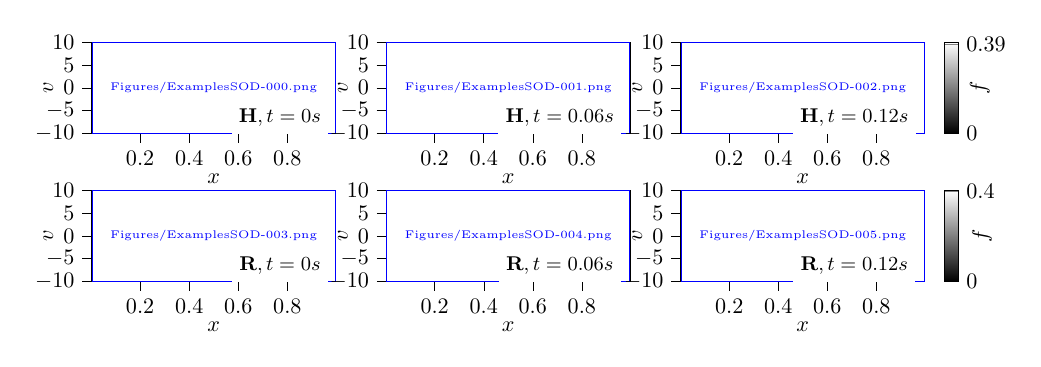
\begin{tikzpicture}[scale=.8]

\begin{groupplot}[group style={group size=3 by 2,horizontal sep=.8cm,vertical sep=0.9cm}]
\nextgroupplot[
tick align=outside,
tick pos=left,
x grid style={white!69.0196078431373!black},
xmin=.0025,xmax=0.9975,
xtick style={color=black},
%y dir=reverse,
y grid style={white!69.0196078431373!black},
ymin=-10,ymax=10,
ytick style={color=black},
width = .45\textwidth,
height = .25\textwidth,
ylabel= $v$,
y label style={yshift=-1.5em},
x label style={yshift=.3em},
xlabel = $x$
]
\addplot graphics [includegraphics cmd=\pgfimage,xmin=.0025,xmax=0.9975, ymin=-10,ymax=10] {Figures/ExamplesSOD-000.png};
\node[fill=white] at (axis cs:.77,-6.5) {\small $\mathbf{H},t=0s$};

\nextgroupplot[
tick align=outside,
tick pos=left,
x grid style={white!69.0196078431373!black},
xmin=.0025,xmax=0.9975,
xtick style={color=black},
%y dir=reverse,
y grid style={white!69.0196078431373!black},
ymin=-10,ymax=10,
ytick style={color=black},
width = .45\textwidth,
height = .25\textwidth,
ylabel= $v$,
y label style={yshift=-1.5em},
x label style={yshift=.3em},
xlabel = $x$
]
\addplot graphics [includegraphics cmd=\pgfimage,xmin=.0025,xmax=0.9975, ymin=-10,ymax=10] {Figures/ExamplesSOD-001.png};
\node[fill=white] at (axis cs:.71,-6.5) {\small $\mathbf{H},t=0.06s$};

\nextgroupplot[
colorbar,
colorbar style={width=1.5ex,ylabel={$f$},ytick={0,0.39},y label style={yshift=2.3em}},
colormap/blackwhite,
point meta max=0.398587408411986,
point meta min=1.61655951012117e-88,
tick align=outside,
tick pos=left,
x grid style={white!69.0196078431373!black},
xmin=.0025,xmax=0.9975,
xtick style={color=black},
%y dir=reverse,
y grid style={white!69.0196078431373!black},
ymin=-10,ymax=10,
ytick style={color=black},
width = .45\textwidth,
height = .25\textwidth,
ylabel= $v$,
y label style={yshift=-1.5em},
x label style={yshift=.3em},
xlabel = $x$
]
\addplot graphics [includegraphics cmd=\pgfimage,xmin=.0025,xmax=0.9975,ymin=-10,ymax=10] {Figures/ExamplesSOD-002.png};
\node[fill=white] at (axis cs:.71,-6.5) {\small $\mathbf{H},t=0.12s$};

\nextgroupplot[
tick align=outside,
tick pos=left,
x grid style={white!69.0196078431373!black},
xmin=.0025,xmax=0.9975,
xtick style={color=black},
%y dir=reverse,
y grid style={white!69.0196078431373!black},
ymin=-10,ymax=10,
ytick style={color=black},
width = .45\textwidth,
height = .25\textwidth,
ylabel= $v$,
y label style={yshift=-1.5em},
x label style={yshift=.3em},
xlabel = $x$
]
\addplot graphics [includegraphics cmd=\pgfimage,xmin=.0025,xmax=0.9975, ymin=-10,ymax=10] {Figures/ExamplesSOD-003.png};
\node[fill=white] at (axis cs:.77,-6.5) {\small $\mathbf{R},t=0s$};

\nextgroupplot[
tick align=outside,
tick pos=left,
x grid style={white!69.0196078431373!black},
xmin=.0025,xmax=0.9975,
xtick style={color=black},
%y dir=reverse,
y grid style={white!69.0196078431373!black},
ymin=-10,ymax=10,
ytick style={color=black},
width = .45\textwidth,
height = .25\textwidth,
ylabel= $v$,
y label style={yshift=-1.5em},
x label style={yshift=.3em},
xlabel = $x$
]
\addplot graphics [includegraphics cmd=\pgfimage,xmin=.0025,xmax=0.9975, ymin=-10,ymax=10] {Figures/ExamplesSOD-004.png};
\node[fill=white] at (axis cs:.71,-6.5) {\small $\mathbf{R},t=0.06s$};
\nextgroupplot[
colorbar,
colorbar style={width=1.5ex,ylabel={$f$},ytick={0,0.4},y label style={yshift=1.7em}},
colormap/blackwhite,
point meta max=0.406101604565777,
point meta min=1.62163282651898e-88,
tick align=outside,
tick pos=left,
x grid style={white!69.0196078431373!black},
xmin=.0025,xmax=0.9975,
xtick style={color=black},
%y dir=reverse,
y grid style={white!69.0196078431373!black},
ymin=-10,ymax=10,
ytick style={color=black},
width = .45\textwidth,
height = .25\textwidth,
ylabel= $v$,
y label style={yshift=-1.5em},
x label style={yshift=.3em},
xlabel = $x$
]
\addplot graphics [includegraphics cmd=\pgfimage,xmin=.0025,xmax=0.9975, ymin=-10,ymax=10] {Figures/ExamplesSOD-005.png};
\node[fill=white] at (axis cs:.71,-6.5) {\small $\mathbf{R},t=0.12s$};
\end{groupplot}

\end{tikzpicture}

		 \caption{Solution $f$ top row for $\mathbf{H}$ and bottom row fro $\mathbf{R}$ in $x$ and $v$.}
	\end{figure}
\end{frame}
%%%%%%%%%%%%%%%%%%%%%%%%%%%%%%%%%%%%%%%%%%%%%%%%%%%%%%%%%%%%%%%%%%%
\section{Model Order Reduction}
\begin{frame}[fragile]{Model Order Reduction}
	\begin{columns}
		\begin{column}{.5\textwidth}
			\begin{figure}
				\subfloat[Evolving the FOM in time.]{\tikzstyle{reco} = [rectangle,minimum height=4em,text centered, fill=blue!20,draw=black]
\begin{tikzpicture}[auto]
	\node [reco,label=FOM] (phys) {$\frac{d}{dt}f = Q(f,t)$};
	\draw [<-,thick] (phys)--+ (-3.5,0) node[midway,above] {input \(t\)};
	\draw [->,thick] (phys)--+ (3.5,0) node[midway,above] {output $f$};
\end{tikzpicture}
}\\
				\subfloat[Evolving the ROM in time.]{\tikzstyle{reco} = [rectangle,minimum height=4em,text centered, fill=blue!20,draw=black]
\begin{tikzpicture}[auto]
	\node [reco,label=ROM] (red) {$\frac{d}{dt}q_n = Q(q_n,t)$};
	\draw [<-,thick] (red)--+ (-3.5,0) node[midway,above] {input \(t\)};
	\draw [->,thick] (red)--+ (3.5,0) node[midway,above] {output $\tilde{f}$};
\end{tikzpicture}
}
				\caption{In the online phase the operator $Q$ is different for the FOM and the ROM.}
			\end{figure}
		\end{column}
		\begin{column}{.5\textwidth}
			\begin{itemize}
				\item<1->\emph{Goal}: Reduce computational cost
				\begin{itemize}
					\item<2->$f(x,v,t)$ with $KJ$ ODE's in time for 1D
				\end{itemize}
				\item<3-> \emph{Require}: Reduction algorithm 
				\begin{itemize}
					\item<4-> Proper Orthogonal Decomposition \emph{(POD)}
					\item<4-> Neural Networks \emph{(NN)}
				\end{itemize}
				\item<5->\emph{Require}: Solution of $f$ (only few timesteps)
				\item<6->\emph{Reduce}: $POD(f(x,v,t))=q(x,n,t)$
				\begin{itemize}
					\item<7->$P$ is \# n with $P<<K$
					\item<8->$KJ$ ODE's vs. $PJ$ ODE's
				\end{itemize}
				\item<9->\emph{Evolve in time}:  $\rightarrow Q(q,t)=\tilde{f}$
				\item<10->\emph{Evaluate mistake}: $f-\tilde{f}<\epsilon$
				
			\end{itemize}
		\end{column}
	\end{columns}
\end{frame}
%%%%%%%%%%%%%%%%%%%%%%%%%%%%%%%%%%%%%%%%%%%%%%%%%%%%%%%%
\section{Proper Orthogonal Decomposotion (POD)}
\begin{frame}[fragile]{Proper Orthogonal Decomposition}
	\only<1,2,3,4>{\begin{itemize}
		\item<1,2,3,4> Solution of a PDE is $f(x,v,t)$ can be obtained
		\begin{itemize}
			\item<2,3,4>Discretization into a system of ODE's
			\item<3,4>Separation of variables ansatz
			\begin{itemize}
				\item<4>$
						f(t,v,x) = \sum_{i=1}^n \tcbhighmath[
						size=title,boxrule=0.4pt,colframe=blue,drop fuzzy shadow=red]{a_i(t)}
						\tcbhighmath[size=title,arc=4pt,drop fuzzy shadow=green]{\Phi_i(x,v)}
						\inlineeqno$
			\end{itemize}
		\end{itemize}
	\end{itemize}}
	\begin{itemize}
		\item<5->How to get $\tcbhighmath[size=title,arc=4pt,drop fuzzy shadow=green]{\Phi_i}$?
		\begin{itemize}
			\item<6->\emph{Preprocessing}: Seperating the spatial and temporal axis of the solution $f(x,v,t)$
			\begin{itemize}
				\item $X=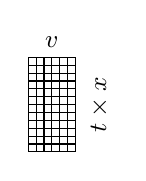
\begin{tikzpicture}[scale=0.1,baseline={([yshift=-.5ex]current bounding box.center)}]
\draw (0,0) grid (6,12);
\node at (3,12) [above] {\small $v$};
\node at (6.7,6) [below, rotate=90]  {\small $t\times x$};
\end{tikzpicture}
$ 
				%\only<8->{\qquad \qquad 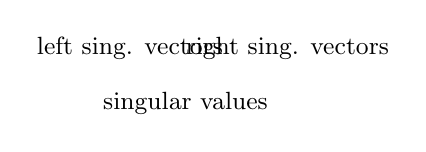
\begin{tikzpicture}[scale=0.1]
\node (sv) at (1,1) {\small singular values};
\node (lv) [above left of=sv]  {\small left sing. vectors};
\node [right of=lv,node distance=2cm]  {\small right sing. vectors};
\end{tikzpicture}
}
			\end{itemize}
			\item<7->\emph{Sigular Value Decomposition}: \qquad 
				$X=
				\tcbhighmath[
				size=title,boxrule=0.5pt,colframe=blue,drop fuzzy shadow=red,title=LSV]{U}
				\tcbhighmath[
				size=title,boxrule=0.4pt,colframe=red,drop fuzzy shadow=blue,title=SV]{\Sigma}
				\tcbhighmath[
				 size=title,boxrule=0.4pt,colframe=green,drop fuzzy shadow=blue,title=RSV]{V^*}\inlineeqno$
			 \item<7->\emph{Truncation}:\qquad 
				 $\tilde{X} = \tcbhighmath[
				 size=title,boxrule=0.5pt,colframe=blue,drop fuzzy shadow=red,title=\Phi]{\tilde{U}}
				 \tilde{\Sigma}\tilde{V^*}\inlineeqno$,
				 \qquad\qquad
				 $\tilde{U}=\Phi=[\Phi_1,\Phi_2,\dots,\Phi_p]\inlineeqno$
			\item<8->\emph{Eckard-Young Theorem}:
				\begin{equation}
					\underset{\tilde{X}, s.t. rank(\tilde{X})=p}{\operatorname{argmin}} \| 
					X -\tilde{X}\|_F
					=\tilde{U}\tilde{\Sigma}\tilde{V}^*
				\end{equation}
		\end{itemize}
	\end{itemize}
\end{frame}
%%%%%%%%%%%%%%%%%%%%%%%%%%%%%%%%%%%%%%%%%%%%%%%%%%%%%%5
\section{Neural Networks}
\begin{frame}[fragile]{Terminology}
	\begin{columns}
		\begin{column}{.5\textwidth}
			\begin{figure}
				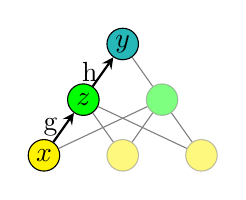
\begin{tikzpicture}
	\node [fill=yellow,circ] (x) {\(x\)};
	\node [circ,draw=gray,fill=yellow,opacity=.5,right of = x] (empt1) {};
	\node [circ,draw=gray,fill=yellow,opacity=.5,right of = empt1] (empt2) {};
	\path (x) -- (empt1) node [fill=green,circ, midway, above=.5cm] (z) {\(z\)};
	\node [fill=green,opacity=.5,circ,draw=gray,right of = z] (hidden1) {};
	\path (z) -- (hidden1) node [fill=BlueGreen,circ,midway, above=.5cm] (y) {\(y\)};
	\draw [arrow] (x)--(z) node [midway,xshift=-1.1ex] {g};
	\draw [arrow] (z)--(y) node [midway,xshift=-1.1ex] {h};
	\draw [gray] (x)--(hidden1);
	\draw [gray] (empt1)--(z);
	\draw [gray] (empt1)--(hidden1);
	\draw [gray] (empt2)--(z);
	\draw [gray] (empt2)--(hidden1);
	\draw [gray] (hidden1)--(y);
\end{tikzpicture}
				\caption{Example of a simple network.}
			\end{figure}
			\begin{itemize}
				\item<1-> Network with three layers
				\begin{itemize}
					\item<2->\colorbox{yellow}{Input layer}
					\item<2-> \colorbox{green}{Hidden layer}
					\item<2-> \colorbox{BlueGreen}{Output layer}
				\end{itemize}
			\end{itemize}
		\end{column}
		\begin{column}{.5\textwidth}
			\begin{itemize}
				\item<3->\emph{Layer}: Stage of computation
				\item<4->\emph{Computations}/ Forward pass
					\begin{itemize}
						\item $g(x)=g(xW+b)=z$
						\item $h(z)=h(zW+b)=y$
						 \begin{itemize}
						 	\item $h(g(x))=y$
						 \end{itemize}
					\end{itemize}
				\item<5->\emph{Neuron}: Entry in 'Tensor'
				\item<6->\emph{Trainable parameters}: $W$, $b$
			\end{itemize}
		\end{column}
	\end{columns}
\end{frame}
\begin{frame}[fragile]{Autoencoders}
	\begin{figure}
		\scalebox{.7}[.7]{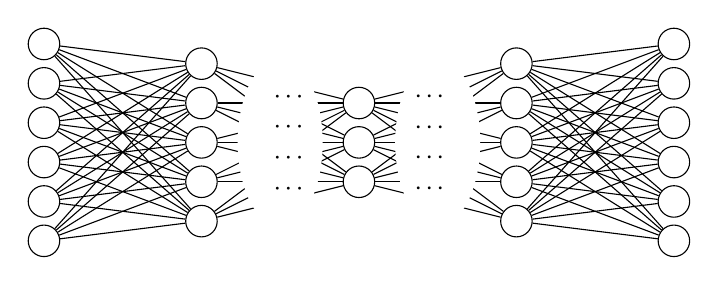
\begin{tikzpicture}

%input layer
\foreach \x [count=\y] in {0,.5,1.0,1.5,2,2.5}
	\node[circ] at (0,\x) (\y) {};
%hidden layer
\foreach \x  [count=\y from 7] in {0.25,0.75,1.25,1.75,2.25}
	\node[circ] at (2,\x) (\y) {};
%code layer
\foreach \x [count=\y from 12] in {0.75,1.25,1.75}
\node[circ] at (4, \x) (\y) {};
%hidden layer
\foreach \x  [count=\y from 15] in {0.25,0.75,1.25,1.75,2.25}
\node[circ] at (6,\x) (\y) {};
%output layer
\foreach \x [count=\y from 20] in {0,.5,1.0,1.5,2,2.5}
\node[circ] at (8, \x)   (\y) {};
\begin{pgfonlayer}{background}
%draw connections
\foreach \x in {1,...,6}
\foreach \y in {7,...,11}
	\draw (\x) -- (\y);
\foreach \x in {7,...,11}
\foreach \y in {12,...,14}
\draw (\x) -- (\y);
\foreach \y in {12,...,14}
\foreach \x in {15,...,19}
\draw (\x) -- (\y);
\foreach \y in {15,...,19}
\foreach \x in {20,...,25}
\draw (\x) -- (\y);
\end{pgfonlayer}
%dots
\path (3,0)--(3,2.5) node[ellipse,rotate=90,midway, fill=white] {\vdots\hspace{0.5em} \vdots\hspace{0.5em} \vdots \hspace{0.5em} \vdots};
%dots
\path (5,0)--(5,2.5) node[ellipse,rotate=270,midway, fill=white] {\vdots\hspace{0.5em} \vdots\hspace{0.5em} \vdots \hspace{0.5em} \vdots};

%\draw [thick,decorate,decoration={brace,mirror,amplitude=5pt}] (-.3,-.5) -- (1.98,-.5) node [midway,below = 8pt,draw=none,rectangle split,rectangle split parts=2] 
%{Encoder:\nodepart{second} \(h(\Pi)=\Phi\)};
%\draw [thick,decorate,decoration={brace,mirror,amplitude=5pt}] (2.02,-.5) -- (4.3,-.5) node [ midway,below= 8pt,draw=none,rectangle split,rectangle split parts=2] {Decoder: \nodepart{second} g(\Phi)=$\tilde{\Pi}$};
%\draw [thick,decorate,decoration={brace,amplitude=3pt}] (-.3,2.75) -- (.3,2.75) node [midway,above = 8pt,draw=none,rectangle split,rectangle split parts=2] 
%{Input \nodepart{second}Layer};
%\draw [thick,decorate,decoration={brace,amplitude=3pt}] (1.7,2) -- (2.3,2) node [midway,above = 8pt,draw=none,rectangle split,rectangle split parts=2] 
%{Hidden \nodepart{second}Layer};
%\draw [thick,decorate,decoration={brace,amplitude=3pt}] (3.7,2.75) -- (4.3,2.75) node [midway,above = 8pt,draw=none,rectangle split,rectangle split parts=2] 
%{Output \nodepart{second}Layer};
\end{tikzpicture}
}
		\caption{A fully connected autoencoder.}
	\end{figure}
	\vspace{-3em}
	\begin{columns}
		\begin{column}{.5\textwidth}
			\begin{itemize}
				\item <2->\emph{Structure}: Encoder \& Decoder
				\item <2->\emph{Layers}: Input-, Output- \emph{and} Code layer
			\end{itemize}
		\end{column}
		\begin{column}{.5\textwidth}
			\begin{itemize}
				\item <2->\emph{Category}: Self-supervised learning
				\item <2->\emph{Main hyperparameters}:\\
					 	Number \& size of hidden layers\\
					 	esp. size of code layer
			\end{itemize}
		\end{column}
	\end{columns}
\end{frame}

\begin{frame}[fragile]{Training}
	\begin{columns}
		\begin{column}{.5\textwidth}
			\begin{figure}
				\scalebox{1}[1]{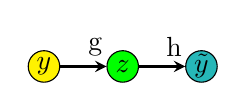
\begin{tikzpicture}
%\tikzstyle{every node} = [font=\footnotesize]
	\node [draw,fill=yellow,circ] (x) {\(y\)};
	\node [draw,fill=green,circ,right of = x] (z) {\(z\)};
	\node [draw,fill=BlueGreen,circ,right of = z] (y) {\(\tilde{y}\)};
	\draw [arrow] (x)--(z) node [midway,above,xshift=1ex] {g};
	\draw [arrow] (z)--(y) node [midway,above,xshift=1ex] {h};
\end{tikzpicture}}
				\caption{A very simple network}
			\end{figure}
		\end{column}
	\begin{column}{.5\textwidth}
		\begin{itemize}
			\item \emph{Forward propagation}: $\tilde{y}=h(z,b)=h((g(y,a)),b) \qquad\inlineeqno$ 
			\item<2-> \emph{Loss function}: $L(y,\tilde{y})=
			\frac{1}{2}(y - \tilde{y})^2 = E\qquad\inlineeqno$
			\item<3-> \emph{Backpropagation}:
			\begin{itemize}
				\item<4-> $\frac{\partial E}{\partial a} =
				-(y - \tilde{y})\frac{\partial y}{\partial z}\frac{\partial z}{\partial a}\qquad\inlineeqno$
				\item<4-> $\frac{\partial E}{\partial b} =
				-(y - \tilde{y})\frac{\partial y}{\partial b}\qquad\inlineeqno$ 
			\end{itemize} 
			\item<5-> \emph{Optimize}:
				\begin{itemize}
					\item<5->$a_{i+1}=a_i + \epsilon \frac{\partial E}{\partial a_i}\qquad\inlineeqno$
					\item<5->$b_{i+1}=b_i + \epsilon \frac{\partial E}{\partial b_i}\qquad\inlineeqno$
				\end{itemize}
			\item<6-> \emph{Hyperparameter}: learning rate $\epsilon$
		\end{itemize}
	\end{column}
	\end{columns}
\end{frame}
\begin{frame}[fragile]{Concepts}
	\begin{columns}
		\begin{column}{.5\textwidth}
			\begin{figure}
				\scalebox{.5}[.5]{% This file was created by tikzplotlib v0.9.6.
\pgfplotsset{
	set layers,% using layers
	mark layer=axis tick labels% defines the layer of the marks
}
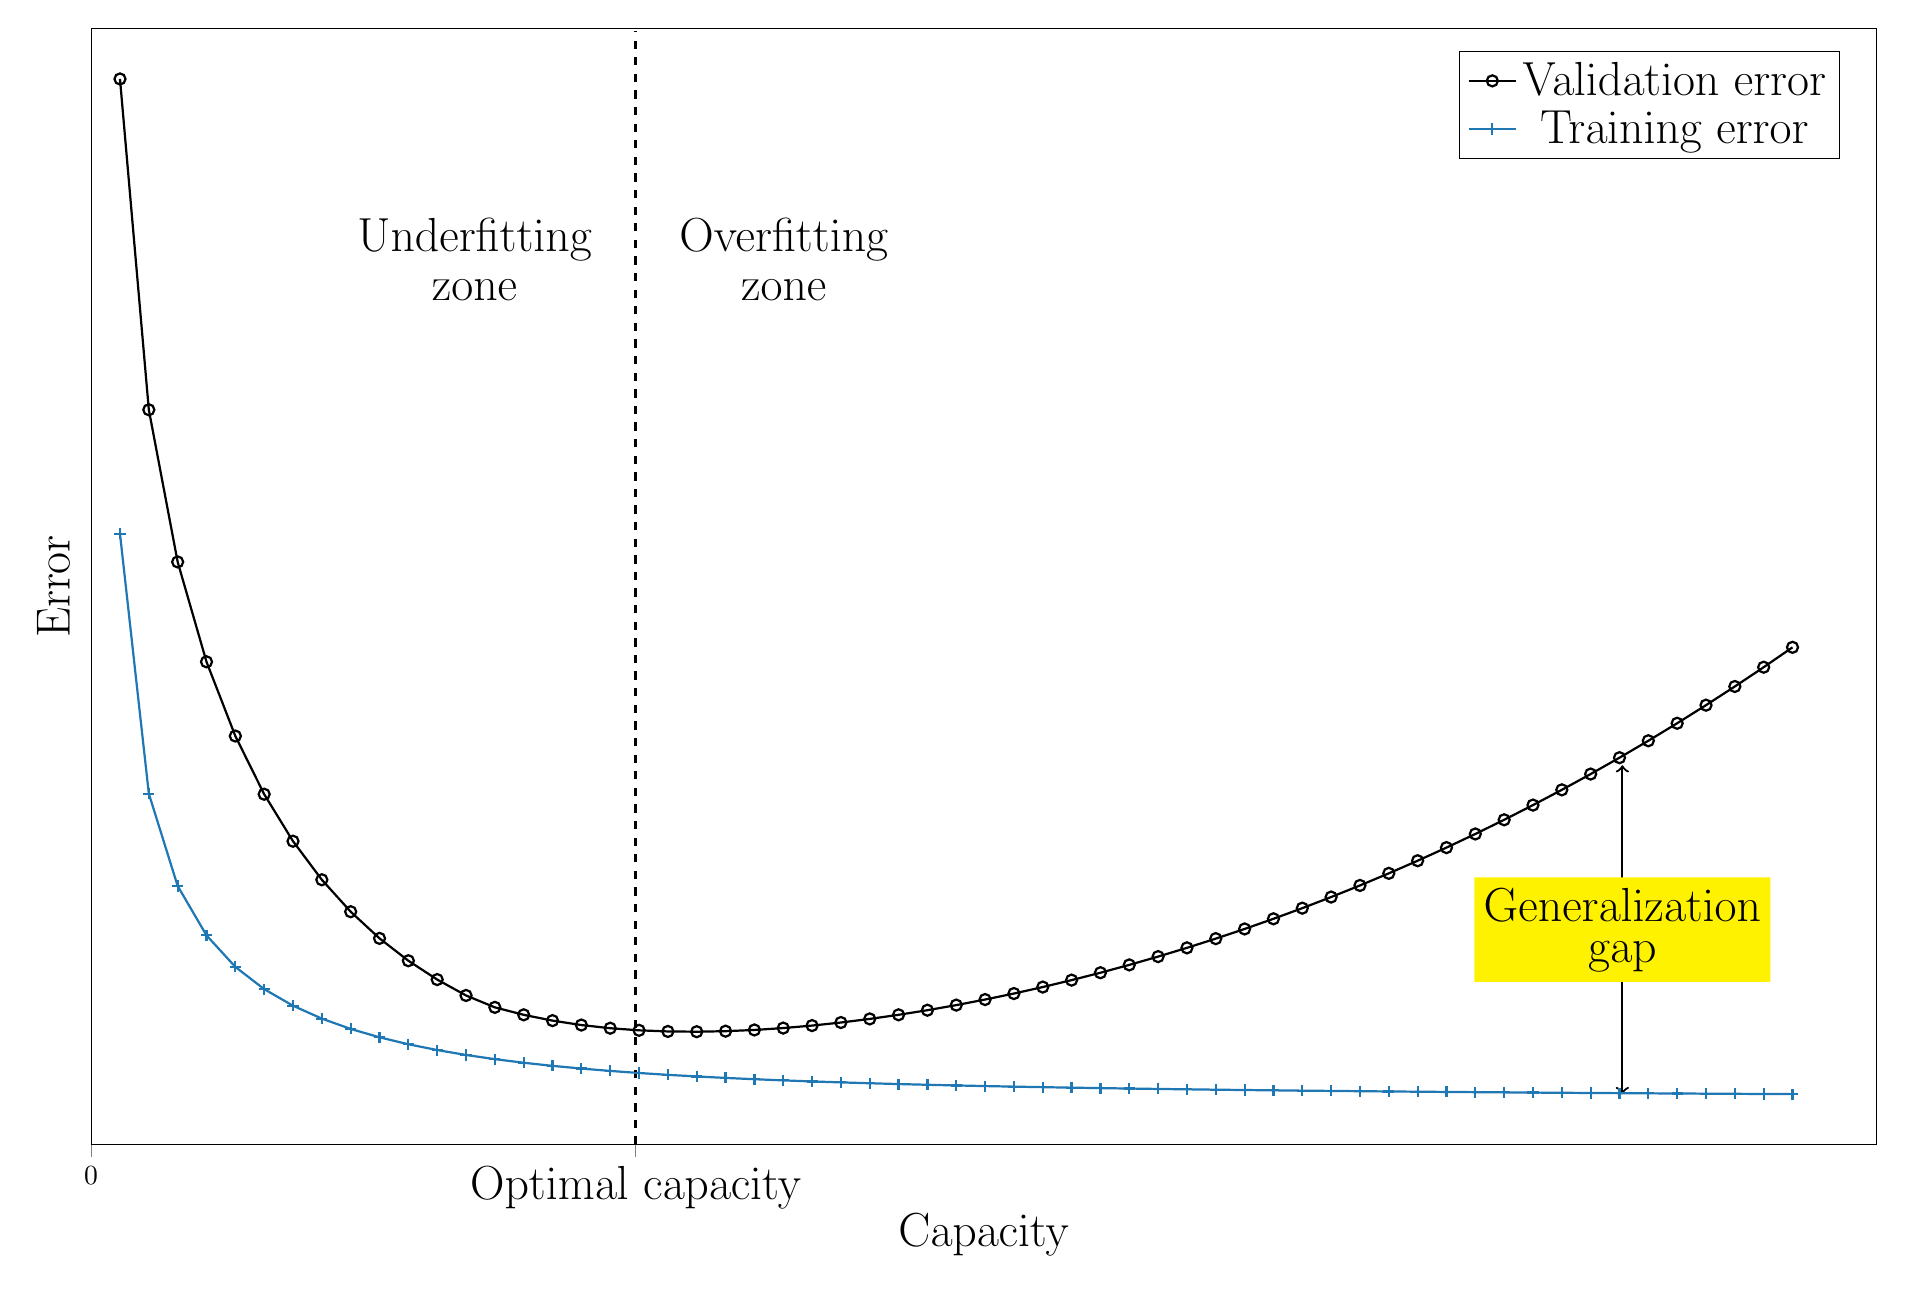
\begin{tikzpicture}
\begin{axis}[
tick align=outside,
tick pos=left,
x grid style={white!69.0196078431373!black},
xlabel={\LARGE Capacity},
xmin=0, xmax=10.4915254237288,
xticklabels = {0,\LARGE Optimal capacity},
xtick={0,3.2},
y grid style={white!69.0196078431373!black},
ylabel={\LARGE Error},
ymin=-0.501805191944399, ymax=12.7389078292872,
ytick=\empty,
ytick style={color=black},
yticklabels = {,,},
width=2\textwidth,
height=1.3\textwidth,
x label style={yshift=.5em},
]
\addplot [thick, black , mark=o, mark size=2, mark options={solid}]
table {%
	0 inf
	0.169491525423729 12.137057237413
	0.338983050847458 8.21466201662695
	0.508474576271186 6.41053580146569
	0.677966101694915 5.22604286369211
	0.847457627118644 4.34623242909512
	1.01694915254237 3.65593083737413
	1.1864406779661 3.09878041398807
	1.35593220338983 2.64171108959936
	1.52542372881356 2.26288853542921
	1.69491525423729 1.94673997609849
	1.86440677966102 1.68157958464115
	2.03389830508475 1.45833647170967
	2.20338983050847 1.26980624712581
	2.3728813559322 1.12866830116967
	2.54237288135593 1.04045080409685
	2.71186440677966 0.971417809099685
	2.88135593220339 0.919088748511067
	3.05084745762712 0.881388366601579
	3.22033898305085 0.856583391159462
	3.38983050847458 0.843229082204998
	3.5593220338983 0.840124118103997
	3.72881355932203 0.846272519273589
	3.89830508474576 0.860851512240569
	4.06779661016949 0.88318440782768
	4.23728813559322 0.912717711615713
	4.40677966101695 0.949001806706436
	4.57627118644068 0.991674651695909
	4.74576271186441 1.04044802361793
	4.91525423728813 1.09509590893097
	5.08474576271186 1.15544470750812
	5.25423728813559 1.22136496682895
	5.42372881355932 1.29276440766818
	5.59322033898305 1.36958203979763
	5.76271186440678 1.45178319763694
	5.93220338983051 1.53935535230884
	6.10169491525424 1.63230457894079
	6.27118644067797 1.73065257694982
	6.44067796610169 1.83443415699726
	6.61016949152542 1.9436951217619
	6.77966101694915 2.05849047904398
	6.94915254237288 2.17888293530334
	7.11864406779661 2.30494162583108
	7.28813559322034 2.43674104458708
	7.45762711864407 2.57436014250381
	7.6271186440678 2.71788156792447
	7.79661016949153 2.86739102695298
	7.96610169491525 3.02297674496113
	8.13559322033898 3.18472901342541
	8.30508474576271 3.35273980873682
	8.47457627118644 3.52710247171199
	8.64406779661017 3.70791143829411
	8.8135593220339 3.89526201341727
	8.98305084745763 4.08925018126187
	9.15254237288136 4.28997244618645
	9.32203389830508 4.49752569951442
	9.49152542372881 4.71200710810794
	9.66101694915254 4.93351402129678
	9.83050847457627 5.16214389326735
	10 5.39799421846945
};
\addlegendentry{\LARGE Validation error}
\addplot [thick, color0, mark=+, mark size=2, mark options={solid}]
table {%
0 inf
0.169491525423729 6.74409390778825
0.338983050847458 3.66249452516524
0.508474576271186 2.56807895469113
0.677966101694915 1.98264844839045
0.847457627118644 1.60850296258454
1.01694915254237 1.34503007352016
1.1864406779661 1.14816315771571
1.35593220338983 0.995206947153229
1.52542372881356 0.873084419642305
1.69491525423729 0.773614788943724
1.86440677966102 0.69135176109086
2.03389830508475 0.622491198528442
2.20338983050847 0.564274344179929
2.3728813559322 0.514640334137393
2.54237288135593 0.472012814370054
2.71186440677966 0.435162870611037
2.88135593220339 0.403117523010918
3.05084745762712 0.375096584488649
3.22033898305085 0.35046783225793
3.38983050847458 0.328714390718848
3.5593220338983 0.309410492762954
3.72881355932203 0.29220313698828
3.89830508474576 0.276797987992008
4.06779661016949 0.262948391470186
4.23728813559322 0.250446716304759
4.40677966101695 0.239117462143469
4.57627118644068 0.228811724792275
4.74576271186441 0.219402718421571
4.91525423728813 0.210782128978517
5.08474576271186 0.202857127402874
5.25423728813559 0.195547910838997
5.42372881355932 0.188785669382798
5.59322033898305 0.182510897943167
5.76271186440678 0.176671989552264
5.93220338983051 0.171224059336657
6.10169491525424 0.16612795835743
6.27118644067797 0.161349444356969
6.44067796610169 0.156858482632537
6.61016949152542 0.152628655174172
6.77966101694915 0.148636660141543
6.94915254237288 0.144861886925093
7.11864406779661 0.141286054604014
7.28813559322034 0.137892903702013
7.45762711864407 0.134667932848111
7.6271186440678 0.131598173349214
7.79661016949153 0.128671995833114
7.96610169491525 0.12587894407168
8.13559322033898 0.123209591881695
8.30508474576271 0.120655419654749
8.47457627118644 0.11820870761199
8.64406779661017 0.115862443333594
8.8135593220339 0.113610241492442
8.98305084745763 0.111446274039436
9.15254237288136 0.109365209354653
9.32203389830508 0.107362159102779
9.49152542372881 0.105432631720052
9.66101694915254 0.103572491619112
9.83050847457627 0.101777923332568
10 0.100045399929762
};
\addlegendentry{\LARGE Training error}

\draw [dashed,thick](axis cs:3.2,-.5) -- (axis cs:3.2,12.7);
\draw (axis cs:3.4,10) node[
	rectangle split, rectangle split parts=2, right]{
		\LARGE Overfitting\nodepart{second}\LARGE zone
	};
\draw (axis cs:3,10) node[
	rectangle split, rectangle split parts=2,left]{
		\LARGE Underfitting\nodepart{second}\LARGE zone
	};
\draw [thick,<->] (axis cs:9,4) -- (axis cs:9,0.1) node[
fill=yellow,rectangle split,midway,rectangle split parts=2] {
	\LARGE Generalization\nodepart{second}\LARGE gap
	};
\end{axis}
\end{tikzpicture}
}
				\caption{Influence of capacity}
			\end{figure}
		\end{column}
		\begin{column}{.5\textwidth}
			\begin{itemize}
				\item \emph{Over- and Underfitting}:
					\begin{itemize}
						\item<2->\emph{Goal}: Reach optimal capacity
					\end{itemize}
				\item<3->\emph{How to direct capacity ?}:
				\begin{itemize}
					\item<4-> Size of the network
					\item<5-> Activation functions
					\item<6-> Loss function
					\item<7-> Data distortion/ add variation to existing data
					\item<8-> ...
					\item<8-> Any other means of regularization
				\end{itemize}
				\item<9->\emph{Initialization}
			\end{itemize}
		\end{column}
	\end{columns}
\end{frame}
%%%%%%%%%%%%%%%%%%%%%%%%%%%%%%%%%%%%%%%%%%%%%%%%%%%%%%%%%%%%%%%%%%%%%
\section{Results}
\begin{frame}[fragile]{Number of intrinsic variables}
	\begin{figure}
		\centering
		\scalebox{.8}[.8]{% This file was created by tikzplotlib v0.9.6.
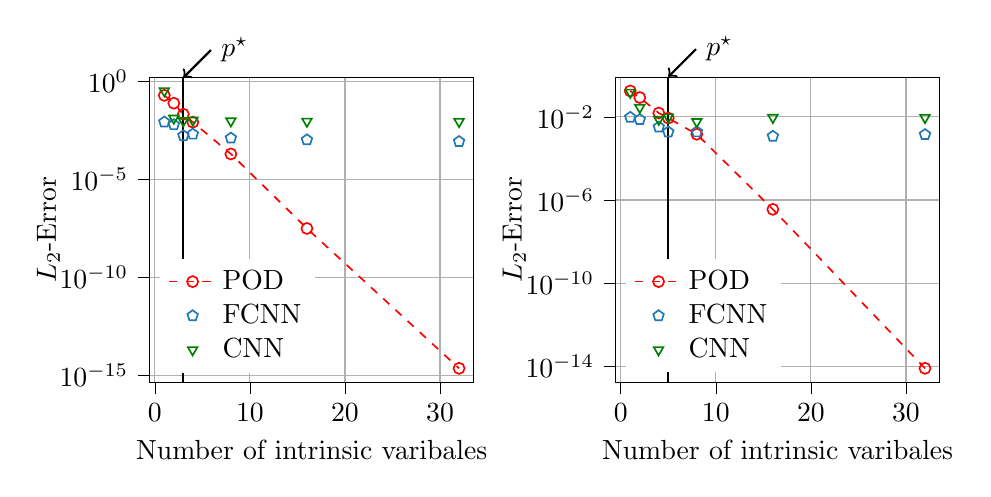
\begin{tikzpicture}
\definecolor{color0}{rgb}{0.12156862745098,0.466666666666667,0.705882352941177}

\begin{groupplot}[group style={group size=2 by 1,horizontal sep=1.8cm}]
\nextgroupplot[
legend cell align={left},
legend style={draw=none,at={(0.03,0.03)}, anchor=south west},
log basis y={10},
tick align=outside,
tick pos=left,
x grid style={white!69.0196078431373!black},
xmajorgrids,
xmin=-0.55, xmax=33.55,
xminorgrids,
xtick style={color=black},
y grid style={white!69.0196078431373!black},
ymajorgrids,
ymin=4.38349387313967e-16, ymax=1.61134858880557,
yminorgrids,
ymode=log,
ytick style={color=black},
xlabel={Number of intrinsic varibales},
ylabel={\(L_2\)-Error},
width=0.47\textwidth,
height =.45\textwidth,
clip=false,
y label style={yshift=-.7em}
]
\addplot [semithick, red, mark=o, mark size=2, mark options={solid}, dashed]
table {%
1 0.188112310801957
2 0.0750338979596223
3 0.020528730333796635
4 0.00808627149114823
8 0.000193252431896578
16 3.06183124046159e-08
32 2.23530701528268e-15
};
\addlegendentry{POD}
\addplot [semithick, color0, mark=pentagon, mark size=2, mark options={solid}, only marks]
table {%
1 0.00824632961302996
2 0.0060168607160449
3 0.0016505243
4 0.00198765122331679
8 0.00124555476941168
16 0.00101344427093863
32 0.000832061574328691
};
\addlegendentry{FCNN}
\addplot [semithick, green!50!black, mark=triangle, mark size=2, mark options={solid,rotate=180}, only marks]
table {%
1 0.315989553928375
2 0.0128393778577447
3 0.00947935
4 0.0101089663803577
8 0.00921880733221769
16 0.00887134857475758
32 0.00860222987830639
};
\addlegendentry{CNN}
\draw[thick](3,40e-17)--(3,1.5);
\draw [thick,<-] (axis cs:3,1.5)-- +(10pt,10pt) node[right] {\(p^\star\)};
\nextgroupplot[
legend cell align={left},
legend style={draw=none, at={(0.03,0.03)}, anchor=south west},
log basis y={10},
tick align=outside,
tick pos=left,
x grid style={white!69.0196078431373!black},
xmajorgrids,
xmin=-0.55, xmax=33.55,
xminorgrids,
xtick style={color=black},
y grid style={white!69.0196078431373!black},
ymajorgrids,
ymin=1.70008814466799e-15, ymax=0.821373329691319,
yminorgrids,
ymode=log,
ytick style={color=black},
xlabel={Number of intrinsic varibales},
ylabel={\(L_2\)-Error},
width=0.47\textwidth,
height =.45\textwidth,
clip=false,
y label style={yshift=-.7em}
]
\addplot [semithick, red, mark=o, mark size=2, mark options={solid}, dashed]
table {%
1 0.176637499442346
2 0.0853532495802733
4 0.015335605212791
5 0.008731715326052242
8 0.00145958547754045
16 3.54159334428613e-07
32 7.90549608414532e-15
};
\addlegendentry{POD}
\addplot [semithick, color0, mark=pentagon, mark size=2, mark options={solid}, only marks]
table {%
1 0.00949728023260832
2 0.00740677583962679
4 0.0032303836196661
5 0.0018827654
8 0.00190045870840549
16 0.00116818200331181
32 0.00140941923018545
};
\addlegendentry{FCNN}
\addplot [semithick, green!50!black, mark=triangle, mark size=2, mark options={solid,rotate=180}, only marks]
table {%
1 0.150382950901985
2 0.0282952953130007
4 0.00750687718391418
5 0.009697513
8 0.00584819912910461
16 0.00925309397280216
32 0.00917380768805742
};
\addlegendentry{CNN}
\draw[thick](5,16.5e-16)--(5,0.85);
\draw [thick,<-] (axis cs:5,0.85)-- +(10pt,10pt) node[right] {\(p^\star\)};
\end{groupplot}

\end{tikzpicture}
}
		\caption{Variation of $p$ for $\mathbf{H}$ left and $\mathbf{R}$ right.}
	\end{figure}
	\begin{itemize}
		\item \emph{Evaluation metric}:
			\begin{equation}
				L_2\text{-Error} = \frac{||f-\tilde{f}||_2}{||f||_2}
			\end{equation}
	\end{itemize}
\end{frame}
\begin{frame}[fragile]{Amount of parameters}
	\begin{table}[htp]
		\centering
		\caption{Amount of parameters used to reconstruct \(f\), the number of intrinsic variables \(p\) and the corresponding $L_2$-Error for POD, the FCNNs, and the CNN.}
		\begin{tabular*}{10cm}{ @{\extracolsep{\fill}} c c c c c c c @{} }
			\toprule
			Algorithm & \multicolumn{2}{c}{Parameters} & \multicolumn{2}{c}{Int. variables \(p\)}& \multicolumn{2}{c}{$\L2$-error} \\ [.5ex]
			& $\mathbf{H}$&$\mathbf{R}$&$\mathbf{H}$&$\mathbf{R}$&$\mathbf{H}$&$\mathbf{R}$\\   
			\hline
			POD     & 15129 & 25225 & 3 & 5 & 0.0205 & 0.0087 \\
			FCNN 	& 2683 & 3725 & 3 & 5 & 0.0008 & 0.0009 \\
			CNN   	& 8246 & 8246 & 5 & 5 &	0.025 & 0.027\\
			\bottomrule
		\end{tabular*} \label{Tab: Parameters}
	\end{table}
\end{frame}
\begin{frame}[fragile]{Time dependece of $L_2$-Error}
	\begin{columns}
		\begin{column}{.61\textwidth}
			\begin{figure}
				\scalebox{.7}[.7]{% This file was created by tikzplotlib v0.9.6.
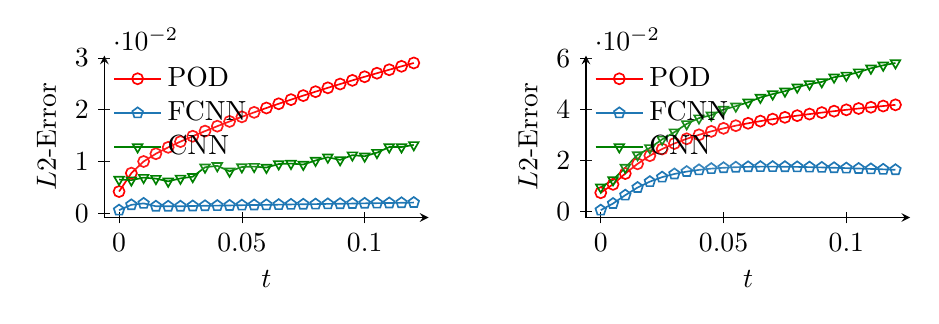
\begin{tikzpicture}
\definecolor{color0}{rgb}{0.12156862745098,0.466666666666667,0.705882352941177}

\begin{groupplot}[group style={group size=2 by 1,horizontal sep=2cm}]
\nextgroupplot[
legend cell align={left},
legend style={fill opacity=0.1,text opacity=1.0,draw=none, at={(0,1)},anchor= north west},
tick align=outside,
tick pos=left,
x grid style={white!69.0196078431373!black},
xmin=-0.006, xmax=0.126,
xtick style={color=black},
y grid style={white!69.0196078431373!black},
ymin=-0.000841513772702749, ymax=0.0304345512636816,
ytick style={color=black},
ylabel={$L2$-Error},
xlabel={\(t\)},
axis lines=left,
width=0.47\textwidth,
height =.3\textwidth,
x tick label style={/pgf/number format/fixed}
]
\addplot [semithick, red, mark=o, mark size=2, mark options={solid}]
table {%
0 0.0041745608742312
0.005 0.00772826090461208
0.01 0.00998129651030254
0.015 0.0114814636830063
0.02 0.0127128633875819
0.025 0.0138212914705674
0.03 0.0148590810264679
0.035 0.0158480900427887
0.04 0.0167989301972853
0.045 0.0177175305866807
0.05 0.0186076563966316
0.055 0.0194719780627452
0.06 0.0203125628459335
0.065 0.021131115773516
0.07 0.0219291044243208
0.075 0.0227078270777979
0.08 0.0234684520909674
0.085 0.0242120420959511
0.09 0.0249395698621951
0.095 0.0256519293912289
0.1 0.0263499442110898
0.105 0.0270343740437529
0.11 0.0277059205812353
0.115 0.0283652327959761
0.12 0.029012911943846
};
\addlegendentry{POD}
\addplot [semithick, color0, mark=pentagon, mark size=2, mark options={solid}]
table {%
0 0.000580125547132904
0.005 0.0016071267939448
0.01 0.00188504649223781
0.015 0.00133036247337402
0.02 0.00132628189845874
0.025 0.00132716953321487
0.03 0.00138970165580601
0.035 0.00142017716840674
0.04 0.00145638808517116
0.045 0.00148681063630736
0.05 0.00153865172400739
0.055 0.0015731085384213
0.06 0.00160068094345799
0.065 0.00164077357612924
0.07 0.00168465107889107
0.075 0.00170978225630885
0.08 0.00174559426233016
0.085 0.00178917826233095
0.09 0.00182042226136015
0.095 0.0018497979559777
0.1 0.00189400391034215
0.105 0.00192810267450896
0.11 0.00196043475749194
0.115 0.00199731114052969
0.12 0.00204309455217968
};
\addlegendentry{FCNN}
\addplot [semithick, green!50!black, mark=triangle, mark size=2, mark options={solid,rotate=180}]
table {%
0 0.00649221194908023
0.005 0.00637732213363051
0.01 0.00686583481729031
0.015 0.00666404515504837
0.02 0.00614608032628894
0.025 0.0067147696390748
0.03 0.00703709293156862
0.035 0.00886726658791304
0.04 0.00913859903812408
0.045 0.00808194372802973
0.05 0.00891359616070986
0.055 0.00899100676178932
0.06 0.00881004240363836
0.065 0.009485456161201
0.07 0.00957572367042303
0.075 0.00939757097512484
0.08 0.0101738022640347
0.085 0.0107985194772482
0.09 0.0102939195930958
0.095 0.0112069239839911
0.1 0.0109974481165409
0.105 0.0116838105022907
0.11 0.0127648552879691
0.115 0.0127696730196476
0.12 0.0131859742105007
};
\addlegendentry{CNN}

\nextgroupplot[
legend cell align={left},
legend style={fill opacity=0.1,text opacity=1.0,draw=none,at={(0,1)},anchor= north west},
tick align=outside,
tick pos=left,
x grid style={white!69.0196078431373!black},
xmin=-0.006, xmax=0.126,
xtick style={color=black},
y grid style={white!69.0196078431373!black},
ymin=-0.00230221234608083, ymax=0.0611092213046212,
ytick style={color=black},
ylabel={$L2$-Error},
xlabel={\(t\)},
axis lines=left,
width=0.47\textwidth,
height =.3\textwidth,
x tick label style={/pgf/number format/fixed}
]
\addplot [semithick, red, mark=o, mark size=2, mark options={solid}]
table {%
0 0.00740144721634158
0.005 0.0106893808997395
0.01 0.0149150434602834
0.015 0.0187372384735488
0.02 0.0219134756297143
0.025 0.0245262733618508
0.03 0.0266961103723662
0.035 0.0285235128498648
0.04 0.0300844182519668
0.045 0.0314352845718027
0.05 0.0326184730907696
0.055 0.0336663066570384
0.06 0.0346038953801234
0.065 0.0354510718869172
0.07 0.0362237260413102
0.075 0.0369347412336944
0.08 0.0375946650603757
0.085 0.038212200327165
0.09 0.0387945721638091
0.095 0.0393478079345977
0.1 0.0398769544960087
0.105 0.0403862495460136
0.11 0.0408792586959919
0.115 0.0413589864772983
0.12 0.0418279671630029
};
\addlegendentry{POD}
\addplot [semithick, color0, mark=pentagon, mark size=2, mark options={solid}]
table {%
0 0.000580125547132904
0.005 0.00316589483113868
0.01 0.00644069989189273
0.015 0.0094435622115595
0.02 0.0117462910277023
0.025 0.0135083335876847
0.03 0.0147541401649302
0.035 0.0156776008463723
0.04 0.016359257000976
0.045 0.0168387643606902
0.05 0.0171780580682302
0.055 0.0174023878750501
0.06 0.0175410884132009
0.065 0.0176139846919089
0.07 0.0176235927054341
0.075 0.0175937947736521
0.08 0.0175227229486254
0.085 0.0174309194625182
0.09 0.0173139350118248
0.095 0.0171816191398723
0.1 0.0170365979594161
0.105 0.0168830016501064
0.11 0.0167221999919594
0.115 0.0165578630537945
0.12 0.0163915040253931
};
\addlegendentry{FCNN}
\addplot [semithick, green!50!black, mark=triangle, mark size=2, mark options={solid,rotate=180}]
table {%
0 0.00956460367888212
0.005 0.0124108670279384
0.01 0.0172932539135218
0.015 0.0221939664334059
0.02 0.0249469373375177
0.025 0.0283007752150297
0.03 0.0311273168772459
0.035 0.0343553461134434
0.04 0.036633376032114
0.045 0.0377688743174076
0.05 0.0399965308606625
0.055 0.041291106492281
0.06 0.0428216233849525
0.065 0.0447116009891033
0.07 0.0460423566401005
0.075 0.0471654385328293
0.08 0.048737995326519
0.085 0.049955528229475
0.09 0.0508080013096333
0.095 0.0526490993797779
0.1 0.053377740085125
0.105 0.0546315461397171
0.11 0.0561474151909351
0.115 0.0573081187903881
0.12 0.0582268834114075
};
\addlegendentry{CNN}
\end{groupplot}

\end{tikzpicture}
}
				\caption{
					Comparison of the $L_2$-Error over time, $\mathbf{H}$ top and $\mathbf{R}$ bottom.}
			\end{figure}
		\end{column}
		\begin{column}{.39\textwidth}
			\begin{itemize}
				\item\emph{POD}:
				\begin{itemize}
					\item $\mathbf{H}$ - lin. increase of $L_2$
					\item $\mathbf{R}$ - increase \& stagnation of $L_2$
				\end{itemize}
				\item\emph{FCNN}:
				\begin{itemize}
					\item $\mathbf{H}$ \& $\mathbf{R}$ - no distinct time dependence $L_2$
					\item biggest value at onset  
				\end{itemize}
				\item\emph{CNN}:
				\begin{itemize}
					\item $\mathbf{H}$ \& $\mathbf{R}$ - similar evolution
				\end{itemize}
			\end{itemize}
		\end{column}
	\end{columns}
\end{frame}
\begin{frame}[fragile]{A detailed look at reconstructions}
	\begin{columns}
		\begin{column}{.61\textwidth}
			\begin{figure}
				\vspace{-.5cm}
				\scalebox{.7}[.7]{% This file was created by tikzplotlib v0.9.6.
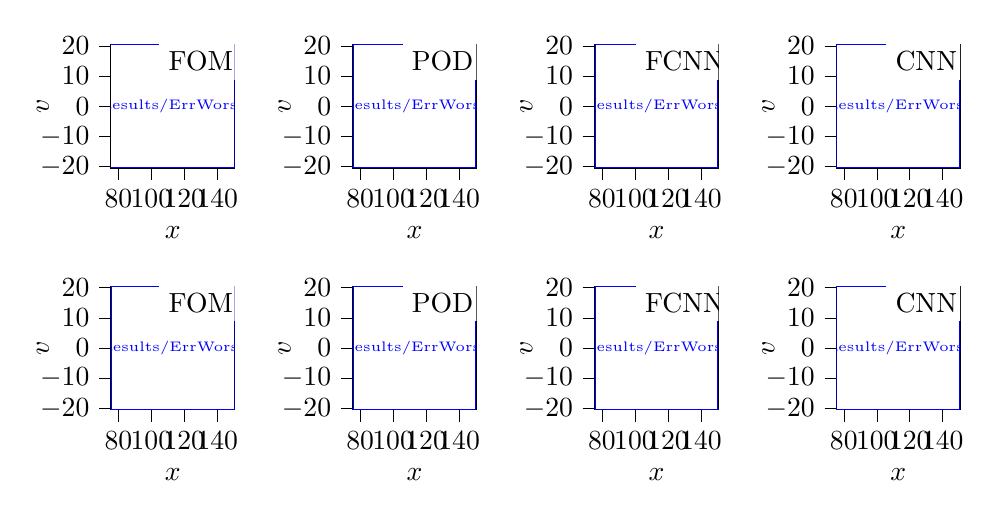
\begin{tikzpicture}

\begin{groupplot}[group style={group size=4 by 2,horizontal sep=1.5cm,vertical sep = 1.5cm}]
\nextgroupplot[
tick align=outside,
tick pos=left,
x grid style={white!69.0196078431373!black},
xmin=75.5, xmax=150.5,
xtick style={color=black},
y grid style={white!69.0196078431373!black},
ymin=-20.5, ymax=20.5,
ytick style={color=black},
height=.26\textwidth,
width=.26\textwidth,
xlabel={\(x\)},
ylabel={\(v\)},
y label style={yshift=-1em}
]
\addplot graphics [includegraphics cmd=\pgfimage,xmin=74.5, xmax=150.5, ymin=-20.5, ymax=20.5] {Figures/Results/ErrWorst-000.png};
\node[fill=white] at (axis cs:130,15) {FOM};
\nextgroupplot[
tick align=outside,
tick pos=left,
x grid style={white!69.0196078431373!black},
xmin=75.5, xmax=150.5,
xtick style={color=black},
y grid style={white!69.0196078431373!black},
ymin=-20.5, ymax=20.5,
ytick style={color=black},
height=.26\textwidth,
width=.26\textwidth,
xlabel={\(x\)},
ylabel={\(v\)},
y label style={yshift=-1em}
]
\addplot graphics [includegraphics cmd=\pgfimage,xmin=75.5, xmax=150.5, ymin=-20.5, ymax=20.55] {Figures/Results/ErrWorst-001.png};
\node[fill=white] at (axis cs:130,15) {POD};
\nextgroupplot[
tick align=outside,
tick pos=left,
x grid style={white!69.0196078431373!black},
xmin=75.5, xmax=150.5,
xtick style={color=black},
y grid style={white!69.0196078431373!black},
ymin=-20.5, ymax=20.5,
ytick style={color=black},
height=.26\textwidth,
width=.26\textwidth,
xlabel={\(x\)},
ylabel={\(v\)},
y label style={yshift=-1em}
]
\addplot graphics [includegraphics cmd=\pgfimage,xmin=75.5, xmax=150.5, ymin=-20.5, ymax=20.55] {Figures/Results/ErrWorst-002.png};
\node[fill=white] at (axis cs:130,15) {FCNN};
\nextgroupplot[
tick align=outside,
tick pos=left,
x grid style={white!69.0196078431373!black},
xmin=75.5, xmax=150.5,
xtick style={color=black},
y grid style={white!69.0196078431373!black},
ymin=-20.5, ymax=20.5,
ytick style={color=black},
height=.26\textwidth,
width=.26\textwidth,
xlabel={\(x\)},
ylabel={\(v\)},
y label style={yshift=-1em}
]
\addplot graphics [includegraphics cmd=\pgfimage,xmin=75.5, xmax=150.5, ymin=-20.5, ymax=20.55] {Figures/Results/ErrWorst-003.png};
\node[fill=white] at (axis cs:130,15) {CNN};
\nextgroupplot[
tick align=outside,
tick pos=left,
x grid style={white!69.0196078431373!black},
xmin=75.5, xmax=150.5,
xtick style={color=black},
y grid style={white!69.0196078431373!black},
ymin=-20.5, ymax=20.5,
ytick style={color=black},
height=.26\textwidth,
width=.26\textwidth,
xlabel={\(x\)},
ylabel={\(v\)},
y label style={yshift=-1em}
]
\addplot graphics [includegraphics cmd=\pgfimage,xmin=75.5, xmax=150.5, ymin=-20.5, ymax=20.55] {Figures/Results/ErrWorst-004.png};
\node[fill=white] at (axis cs:130,15) {FOM};
\nextgroupplot[
tick align=outside,
tick pos=left,
x grid style={white!69.0196078431373!black},
xmin=75.5, xmax=150.5,
xtick style={color=black},
y grid style={white!69.0196078431373!black},
ymin=-20.5, ymax=20.5,
ytick style={color=black},
height=.26\textwidth,
width=.26\textwidth,
xlabel={\(x\)},
ylabel={\(v\)},
y label style={yshift=-1em}
]
\addplot graphics [includegraphics cmd=\pgfimage,xmin=75.5, xmax=150.5, ymin=-20.5, ymax=20.5] {Figures/Results/ErrWorst-005.png};
\node[fill=white] at (axis cs:130,15) {POD};
\nextgroupplot[
tick align=outside,
tick pos=left,
x grid style={white!69.0196078431373!black},
xmin=75.5, xmax=150.5,
xtick style={color=black},
y grid style={white!69.0196078431373!black},
ymin=-20.5, ymax=20.5,
ytick style={color=black},
height=.26\textwidth,
width=.26\textwidth,
xlabel={\(x\)},
ylabel={\(v\)},
y label style={yshift=-1em}
]
\addplot graphics [includegraphics cmd=\pgfimage,xmin=75.5, xmax=150.5, ymin=-20.5, ymax=20.5] {Figures/Results/ErrWorst-006.png};
\node[fill=white] at (axis cs:130,15) {FCNN};
\nextgroupplot[
tick align=outside,
tick pos=left,
x grid style={white!69.0196078431373!black},
xmin=75.5, xmax=150.5,
xtick style={color=black},
y grid style={white!69.0196078431373!black},
ymin=-20.5, ymax=20.5,
ytick style={color=black},
height=.26\textwidth,
width=.26\textwidth,
xlabel={\(x\)},
ylabel={\(v\)},
y label style={yshift=-1em}
]
\addplot graphics [includegraphics cmd=\pgfimage,xmin=75.5, xmax=150.5, ymin=-20.5, ymax=20.5] {Figures/Results/ErrWorst-007.png};
\node[fill=white] at (axis cs:130,15) {CNN};
\end{groupplot}

\end{tikzpicture}
}
				\caption{
					Comparision of $f$ and $\tilde{f}$ at $t=t_{end}$ and $x\in[0.375,0.75]$, $\mathbf{H}$ top and $\mathbf{R}$ bottom.}
			\end{figure}
		\end{column}
		\begin{column}{.39\textwidth}
			\begin{itemize}
				\item\emph{POD}:
				\begin{itemize}
					\item $\mathbf{H}$ - defective after $x=0.6$: Errors in temperature
					\item $\mathbf{R}$ - almost exact
				\end{itemize}
				\item\emph{FCNN}:
				\begin{itemize}
					\item $\mathbf{H}$ \& $\mathbf{R}$ - almost exact 
				\end{itemize}
				\item\emph{CNN}:
				\begin{itemize}
					\item $\mathbf{H}$ \& $\mathbf{R}$ - average of $\mathbf{H}$ \& $\mathbf{R}$
				\end{itemize}
			\end{itemize}
		\end{column}
	\end{columns}
\end{frame}
\begin{frame}[fragile]{Moments of $f$ and $\tilde{f}$}
	\begin{columns}
		\begin{column}{.61\textwidth}
			\begin{figure}
				\scalebox{.7}[.7]{% This file was created by tikzplotlib v0.9.6.
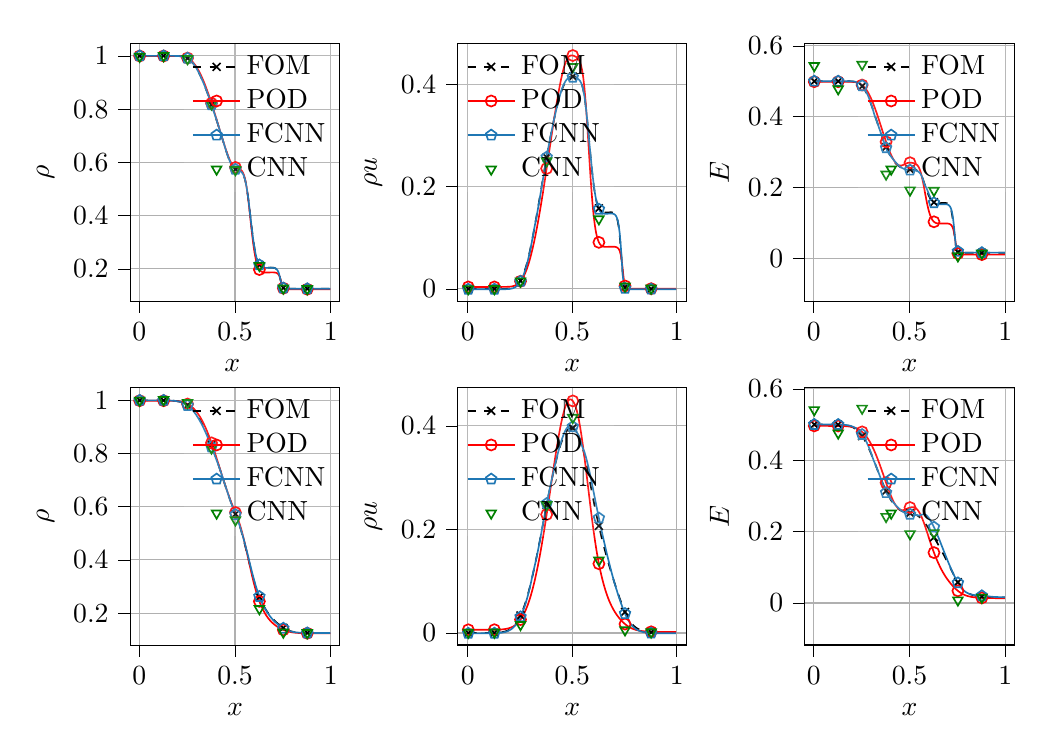
\begin{tikzpicture}

\definecolor{color0}{rgb}{0.12156862745098,0.466666666666667,0.705882352941177}

\begin{groupplot}[group style={group size=3 by 2,horizontal sep=1.5cm,vertical sep=1.1cm}]
\nextgroupplot[
legend cell align={left},
legend style={at={(1,1)},anchor=north east,fill opacity=0.1, draw opacity=1, text opacity=1,draw=none},
tick align=outside,
tick pos=left,
x grid style={white!69.0196078431373!black},
xmajorgrids,
xlabel={\(x\)},
xmin=-0.04725, xmax=1.04725,
xtick style={color=black},
y grid style={white!69.0196078431373!black},
ymajorgrids,
ylabel={\(\rho\)},
ymin=0.0787652333577474, ymax=1.04575335673797,
ytick style={color=black},
width=.35\textwidth,
height=.4\textwidth,
x label style={xshift=-.10em}
]
\addplot [semithick, black, dashed, mark=x,mark size=2,mark repeat=25, mark options={solid}]
table {%
0.0025 0.999999963320219
0.0075 0.999999963320219
0.0125 0.999999963320219
0.0175 0.999999963320219
0.0225 0.999999963320219
0.0275 0.999999963320219
0.0325 0.999999963320219
0.0375 0.999999963320219
0.0425 0.999999963320219
0.0475 0.999999963320219
0.0525 0.999999963320219
0.0575 0.999999963320219
0.0625 0.999999963320219
0.0675 0.999999963320219
0.0725 0.999999963320219
0.0775 0.999999963320219
0.0825 0.999999963320219
0.0875 0.999999963320219
0.0925 0.999999963320219
0.0975 0.999999963320219
0.1025 0.999999963320219
0.1075 0.999999963320219
0.1125 0.999999963320219
0.1175 0.99999990218725
0.1225 0.999999779921312
0.1275 0.999999535389436
0.1325 0.999999413123497
0.1375 0.999998862926777
0.1425 0.99999800706521
0.1475 0.999996539873955
0.1525 0.999994400220039
0.1575 0.99999067110893
0.1625 0.999984741210937
0.1675 0.99997538786668
0.1725 0.999960654821151
0.1775 0.999938524686373
0.1825 0.999904779287485
0.1875 0.999854833651812
0.1925 0.999782024285732
0.1975 0.999676814446082
0.2025 0.999528261331411
0.2075 0.999321570763221
0.2125 0.99903846398378
0.2175 0.998657727852846
0.2225 0.998153625390468
0.2275 0.997497362968249
0.2325 0.99665702917637
0.2375 0.995598572951097
0.2425 0.994286231505565
0.2475 0.992684731116662
0.2525 0.990759225992056
0.2575 0.988477988120837
0.2625 0.985812468406482
0.2675 0.982738213661389
0.2725 0.979236639462984
0.2775 0.975294846754808
0.2825 0.970904521453075
0.2875 0.966063951834654
0.2925 0.960775827750181
0.2975 0.955047118358123
0.3025 0.948889010991806
0.3075 0.94231550510113
0.3125 0.935342617523976
0.3175 0.927988627018073
0.3225 0.920272118005997
0.3275 0.912212653037829
0.3325 0.903829550131773
0.3375 0.895142555236816
0.3425 0.886169641445845
0.3475 0.876929209782527
0.3525 0.867438438611153
0.3575 0.857713405902569
0.3625 0.84776915036715
0.3675 0.837620466183393
0.3725 0.827280374673697
0.3775 0.816761958293426
0.3825 0.806076526641846
0.3875 0.79523612291385
0.3925 0.784251078581199
0.3975 0.773132764376127
0.4025 0.761891756302271
0.4075 0.750539363958897
0.4125 0.739087813939804
0.4175 0.72755067776411
0.4225 0.715944155668601
0.4275 0.704287198873667
0.4325 0.692604199433938
0.4375 0.680926212897667
0.4425 0.669293831556271
0.4475 0.657760913555439
0.4525 0.646399901463435
0.4575 0.635307385371282
0.4625 0.624610216189653
0.4675 0.614472535940317
0.4725 0.605094983027532
0.4775 0.59670429963332
0.4825 0.589521603706555
0.4875 0.583707980620555
0.4925 0.579297664837959
0.4975 0.576156347225874
0.5025 0.574000982137827
0.5075 0.572480116135035
0.5125 0.571264242514586
0.5175 0.570086332467886
0.5225 0.568721416669014
0.5275 0.566925146640875
0.5325 0.564365814893674
0.5375 0.560570557912191
0.5425 0.554906038137583
0.5475 0.546613473158616
0.5525 0.534909016046769
0.5575 0.519142212011875
0.5625 0.498978602580535
0.5675 0.474548706641564
0.5725 0.446512118363992
0.5775 0.416003312820043
0.5825 0.384466831500714
0.5875 0.353428247647408
0.5925 0.324264611953344
0.5975 0.298031599093706
0.6025 0.275379786124596
0.6075 0.256558289894691
0.6125 0.241481600663601
0.6175 0.229826477857736
0.6225 0.221130557549305
0.6275 0.21487615047357
0.6325 0.210551619529724
0.6375 0.207691956789066
0.6425 0.205900455132509
0.6475 0.204856793085734
0.6525 0.204314497800974
0.6575 0.204092799088894
0.6625 0.204064494524247
0.6675 0.204143249071561
0.6725 0.204271674156189
0.6775 0.204410170897459
0.6825 0.204527209966611
0.6875 0.204589748993898
0.6925 0.204552182784447
0.6975 0.20434177838839
0.7025 0.203837538376833
0.7075 0.202838136599614
0.7125 0.201017092435788
0.7175 0.197870639654306
0.7225 0.192691668485984
0.7275 0.184667370258233
0.7325 0.173289806414873
0.7375 0.159203853362646
0.7425 0.144954935098306
0.7475 0.134090918761033
0.7525 0.12823774264409
0.7575 0.125970038083883
0.7625 0.125265816847483
0.7675 0.125069113878103
0.7725 0.125016333200993
0.7775 0.125002356675955
0.7825 0.124998665772952
0.7875 0.12499770292869
0.7925 0.124997443113572
0.7975 0.124997389622224
0.8025 0.124997374338981
0.8075 0.12499736669736
0.8125 0.12499736669736
0.8175 0.12499736669736
0.8225 0.12499736669736
0.8275 0.12499736669736
0.8325 0.12499736669736
0.8375 0.12499736669736
0.8425 0.12499736669736
0.8475 0.12499736669736
0.8525 0.12499736669736
0.8575 0.12499736669736
0.8625 0.12499736669736
0.8675 0.12499736669736
0.8725 0.12499736669736
0.8775 0.12499736669736
0.8825 0.12499736669736
0.8875 0.12499736669736
0.8925 0.12499736669736
0.8975 0.12499736669736
0.9025 0.12499736669736
0.9075 0.12499736669736
0.9125 0.12499736669736
0.9175 0.12499736669736
0.9225 0.12499736669736
0.9275 0.12499736669736
0.9325 0.12499736669736
0.9375 0.12499736669736
0.9425 0.12499736669736
0.9475 0.12499736669736
0.9525 0.12499736669736
0.9575 0.12499736669736
0.9625 0.12499736669736
0.9675 0.12499736669736
0.9725 0.12499736669736
0.9775 0.12499736669736
0.9825 0.12499736669736
0.9875 0.12499736669736
0.9925 0.12499736669736
0.9975 0.12499736669736
};
\addlegendentry{FOM}
\addplot [semithick, red, mark=o,mark size=2, mark repeat=25, mark options={solid}]
table {%
0.0025 0.999548771594793
0.0075 0.999548771594787
0.0125 0.999548771594777
0.0175 0.999548771594753
0.0225 0.999548771594688
0.0275 0.99954877159453
0.0325 0.999548771594179
0.0375 0.999548771593437
0.0425 0.999548771591852
0.0475 0.999548771588456
0.0525 0.999548771581279
0.0575 0.999548771566277
0.0625 0.999548771535268
0.0675 0.999548771471879
0.0725 0.999548771343803
0.0775 0.999548771088022
0.0825 0.999548770583062
0.0875 0.999548769597802
0.0925 0.999548767698169
0.0975 0.99954876407943
0.1025 0.999548757269338
0.1075 0.999548744610781
0.1125 0.999548721373772
0.1175 0.999548679255706
0.1225 0.999548603890035
0.1275 0.999548470777807
0.1325 0.999548238760097
0.1375 0.999547839734983
0.1425 0.999547162765054
0.1475 0.999546030000005
0.1525 0.999544160954158
0.1575 0.999541120663193
0.1625 0.999536246184591
0.1675 0.999528544966733
0.1725 0.999516558049316
0.1775 0.999498181231678
0.1825 0.999470438699194
0.1875 0.999429206591679
0.1925 0.9993688890128
0.1975 0.999282056142071
0.2025 0.99915906311425
0.2075 0.998987678260307
0.2125 0.998752758572666
0.2175 0.998436016733616
0.2225 0.998015925419097
0.2275 0.997467798986495
0.2325 0.996764079322538
0.2375 0.99587483249879
0.2425 0.994768438710398
0.2475 0.993412433898535
0.2525 0.991774442038987
0.2575 0.989823126091609
0.2625 0.98752908500575
0.2675 0.984865633633234
0.2725 0.981809419515683
0.2775 0.978340851622089
0.2825 0.9744443373183
0.2875 0.970108341936711
0.2925 0.965325298291781
0.2975 0.960091400703041
0.3025 0.954406319994776
0.3075 0.94827287369326
0.3125 0.941696680663758
0.3175 0.934685823088954
0.3225 0.927250532091985
0.3275 0.91940290722078
0.3325 0.911156674872146
0.3375 0.902526986722904
0.3425 0.893530256338715
0.3475 0.884184030229781
0.3525 0.874506888547891
0.3575 0.864518370193878
0.3625 0.854238917174887
0.3675 0.843689833494142
0.3725 0.832893254596429
0.3775 0.821872124393158
0.3825 0.810650178169559
0.3875 0.799251931294829
0.3925 0.78770267574189
0.3975 0.77602848917673
0.4025 0.764256265096905
0.4075 0.752413777619085
0.4125 0.740529801647178
0.4175 0.728634319137727
0.4225 0.716758856123944
0.4275 0.70493701438836
0.4325 0.693205287449573
0.4375 0.681604283152755
0.4425 0.670180511628393
0.4475 0.65898892591229
0.4525 0.648096390752349
0.4575 0.637586127827967
0.4625 0.627562790490795
0.4675 0.618156902786947
0.4725 0.609525670234001
0.4775 0.6018447263329
0.4825 0.595283734240775
0.4875 0.589962041804688
0.4925 0.585893694609532
0.4975 0.582950451517276
0.5025 0.580875840796191
0.5075 0.579352251627723
0.5125 0.578077723544553
0.5175 0.576800623627844
0.5225 0.575296690289324
0.5275 0.573308767286148
0.5325 0.570477432918538
0.5375 0.566285778369634
0.5425 0.560040704121852
0.5475 0.550913667192523
0.5525 0.538054899617929
0.5575 0.52077187876436
0.5625 0.49873191332678
0.5675 0.472125596353103
0.5725 0.441728225170466
0.5775 0.408825407012185
0.5825 0.3750163990988
0.5875 0.341952318250269
0.5925 0.311085403139529
0.5975 0.28349274631892
0.6025 0.259803155850325
0.6075 0.240218452263519
0.6125 0.224596872533648
0.6175 0.21256136281911
0.6225 0.203604094956206
0.6275 0.197171596305905
0.6325 0.192725777382
0.6375 0.189782476887888
0.6425 0.187931638026962
0.6475 0.18684363567553
0.6525 0.186265936683102
0.6575 0.186013763883529
0.6625 0.185957830374123
0.6675 0.186011486873066
0.6725 0.186118822997236
0.6775 0.186244486244602
0.6825 0.186365323201625
0.6875 0.186463437237978
0.6925 0.18651985312962
0.6975 0.186507573177517
0.7025 0.186382227399486
0.7075 0.186067492116135
0.7125 0.185430535378378
0.7175 0.18423927878628
0.7225 0.18208804768065
0.7275 0.178277990908776
0.7325 0.171696753937413
0.7375 0.161099168034382
0.7425 0.147018646050487
0.7475 0.134243307515287
0.7525 0.127109461113498
0.7575 0.124412936576949
0.7625 0.123592848531648
0.7675 0.123365803728222
0.7725 0.123305048460296
0.7775 0.123288975392124
0.7825 0.123284741006781
0.7875 0.123283627872577
0.7925 0.123283335737192
0.7975 0.123283259191473
0.8025 0.123283239168794
0.8075 0.123283233940817
0.8125 0.123283232578456
0.8175 0.123283232224191
0.8225 0.123283232132279
0.8275 0.123283232108493
0.8325 0.123283232102354
0.8375 0.123283232100774
0.8425 0.123283232100368
0.8475 0.123283232100264
0.8525 0.123283232100238
0.8575 0.123283232100232
0.8625 0.12328323210023
0.8675 0.12328323210023
0.8725 0.12328323210023
0.8775 0.12328323210023
0.8825 0.12328323210023
0.8875 0.123283232100229
0.8925 0.123283232100229
0.8975 0.123283232100229
0.9025 0.123283232100229
0.9075 0.123283232100229
0.9125 0.123283232100229
0.9175 0.123283232100229
0.9225 0.123283232100229
0.9275 0.123283232100229
0.9325 0.123283232100229
0.9375 0.123283232100229
0.9425 0.123283232100229
0.9475 0.123283232100229
0.9525 0.123283232100229
0.9575 0.123283232100229
0.9625 0.123283232100229
0.9675 0.123283232100229
0.9725 0.123283232100229
0.9775 0.123283232100229
0.9825 0.123283232100229
0.9875 0.123283232100229
0.9925 0.123283232100229
0.9975 0.123283232100229
};
\addlegendentry{POD}
\addplot [semithick, color0, mark=pentagon,mark size=2, mark repeat=25, mark options={solid}]
table {%
0.0025 0.999939968236364
0.0075 0.999939968236364
0.0125 0.999939968236364
0.0175 0.999939968236364
0.0225 0.999939968236364
0.0275 0.999939968236364
0.0325 0.999939968236364
0.0375 0.999939968236364
0.0425 0.999939968236364
0.0475 0.999939968236364
0.0525 0.999939968236364
0.0575 0.999939968236364
0.0625 0.999939968236364
0.0675 0.999939968236364
0.0725 0.999939968236364
0.0775 0.999939968236364
0.0825 0.999939968236364
0.0875 0.999939968236364
0.0925 0.999939968236364
0.0975 0.999939891820153
0.1025 0.999939896596166
0.1075 0.999939795822287
0.1125 0.999939862208871
0.1175 0.999939878924917
0.1225 0.999939654452296
0.1275 0.999939597617739
0.1325 0.999939325504387
0.1375 0.999938859007297
0.1425 0.999938065592104
0.1475 0.999936676130463
0.1525 0.999934615400166
0.1575 0.99993094897423
0.1625 0.999925315666657
0.1675 0.999916495683675
0.1725 0.999902459816673
0.1775 0.999881169782617
0.1825 0.999849121898222
0.1875 0.999801299439218
0.1925 0.999731557825819
0.1975 0.999631308472882
0.2025 0.999489218020477
0.2075 0.99929166957736
0.2125 0.999021155353731
0.2175 0.998656816828327
0.2225 0.998174267319532
0.2275 0.997545471391044
0.2325 0.996739041681091
0.2375 0.995721569260917
0.2425 0.994457296358469
0.2475 0.992910082046038
0.2525 0.991043596862791
0.2575 0.988823653509219
0.2625 0.986217566264363
0.2675 0.983196732779153
0.2725 0.979736232055494
0.2775 0.97581622369874
0.2825 0.971420934805885
0.2875 0.966540744456534
0.2925 0.961170660761686
0.2975 0.955310777331201
0.3025 0.948965688092777
0.3075 0.942144474396721
0.3125 0.934979659743989
0.3175 0.927785223421569
0.3225 0.920081615734559
0.3275 0.911964373543667
0.3325 0.903547288229068
0.3375 0.89501510720509
0.3425 0.886130499390837
0.3475 0.876919190662029
0.3525 0.867408619692119
0.3575 0.857626938571532
0.3625 0.847603971950519
0.3675 0.83736945851109
0.3725 0.826953578955279
0.3775 0.816385962594396
0.3825 0.805695764362239
0.3875 0.795205382224268
0.3925 0.784419378480659
0.3975 0.773457267727607
0.4025 0.762336483129706
0.4075 0.751073205819688
0.4125 0.739683521887622
0.4175 0.728183065732129
0.4225 0.716587809296564
0.4275 0.70491533439893
0.4325 0.693185986616673
0.4375 0.681425008612374
0.4425 0.669666346855079
0.4475 0.657956207720324
0.4525 0.646394694056839
0.4575 0.635514160952507
0.4625 0.624949089251459
0.4675 0.61485644382162
0.4725 0.605438914961922
0.4775 0.596935878722713
0.4825 0.589592156525797
0.4875 0.583598525979771
0.4925 0.579017400860977
0.4975 0.575732599036434
0.5025 0.573749198482778
0.5075 0.572390212462499
0.5125 0.571257876685988
0.5175 0.570111481043009
0.5225 0.568769076743569
0.5275 0.567027286339838
0.5325 0.564539783920806
0.5375 0.560837504334557
0.5425 0.555283192258615
0.5475 0.547092540117984
0.5525 0.535416085249147
0.5575 0.519480185392193
0.5625 0.499157757044603
0.5675 0.475012445105956
0.5725 0.446823057360374
0.5775 0.41563895650399
0.5825 0.384757045704203
0.5875 0.353900500788138
0.5925 0.324724445549341
0.5975 0.298561543727723
0.6025 0.275809307439396
0.6075 0.256807394086932
0.6125 0.241533189128416
0.6175 0.22969940975786
0.6225 0.220858842397156
0.6275 0.214495856362658
0.6325 0.210094252266945
0.6375 0.207182188661626
0.6425 0.205356042282895
0.6475 0.204289610354373
0.6525 0.203732133437044
0.6575 0.203499824692232
0.6625 0.203463445441463
0.6675 0.203535807772707
0.6725 0.203659435710273
0.6775 0.203795783603803
0.6825 0.20391557747737
0.6875 0.203990367575525
0.6925 0.203982203339155
0.6975 0.203831830444053
0.7025 0.203439521794327
0.7075 0.202635776681396
0.7125 0.201135637978904
0.7175 0.198469977133358
0.7225 0.193903454674933
0.7275 0.186410662837518
0.7325 0.174961739386886
0.7375 0.159579780645286
0.7425 0.144058139158938
0.7475 0.133231449872255
0.7525 0.127834568922527
0.7575 0.125873483574161
0.7625 0.125272463028056
0.7675 0.125032803998926
0.7725 0.124968871569786
0.7775 0.124951929856951
0.7825 0.124947448762564
0.7875 0.12494626478889
0.7925 0.124945930467966
0.7975 0.124945836858107
0.8025 0.124945856678562
0.8075 0.124945856678562
0.8125 0.124945856678562
0.8175 0.124945822052467
0.8225 0.124945822052467
0.8275 0.124945822052467
0.8325 0.124945822052467
0.8375 0.124945822052467
0.8425 0.124945822052467
0.8475 0.124945822052467
0.8525 0.124945822052467
0.8575 0.124945822052467
0.8625 0.124945822052467
0.8675 0.124945822052467
0.8725 0.124945822052467
0.8775 0.124945822052467
0.8825 0.124945822052467
0.8875 0.124945822052467
0.8925 0.124945822052467
0.8975 0.124945822052467
0.9025 0.124945822052467
0.9075 0.124945822052467
0.9125 0.124945822052467
0.9175 0.124945822052467
0.9225 0.124945822052467
0.9275 0.124945822052467
0.9325 0.124945822052467
0.9375 0.124945822052467
0.9425 0.124945822052467
0.9475 0.124945822052467
0.9525 0.124945822052467
0.9575 0.124945822052467
0.9625 0.124945822052467
0.9675 0.124945822052467
0.9725 0.124945822052467
0.9775 0.124945822052467
0.9825 0.124945822052467
0.9875 0.124945822052467
0.9925 0.124945857633765
0.9975 0.124945857633765
};
\addlegendentry{FCNN}
\addplot [semithick, green!50!black, mark=triangle,mark size=2, mark repeat=25, mark options={solid,rotate=180}, only marks]
table {%
0.0025 0.997826564006316
0.0075 0.999634082500751
0.0125 0.999670150952461
0.0175 1.00089586698092
0.0225 1.00048700968424
0.0275 0.999750051742945
0.0325 1.00179935112978
0.0375 0.998835991590451
0.0425 1.00054997664232
0.0475 1.00057424643101
0.0525 0.997986365587283
0.0575 0.998990902533898
0.0625 1.00076326957116
0.0675 1.00147754718096
0.0725 0.999688368577223
0.0775 0.999325605539175
0.0825 1.00170001005515
0.0875 1.00006812658065
0.0925 1.00029890353863
0.0975 0.999496227655655
0.1025 0.997886718847813
0.1075 0.999347613408015
0.1125 1.00085362409934
0.1175 1.00004006654788
0.1225 0.999976182595277
0.1275 1.00009961005969
0.1325 1.00124609776032
0.1375 1.00066771874061
0.1425 1.00034903257321
0.1475 0.999733912639129
0.1525 0.99842383311345
0.1575 0.999465783437093
0.1625 1.00011764428554
0.1675 1.00016074302869
0.1725 0.999795045608129
0.1775 1.00020836561154
0.1825 1.00125098839784
0.1875 1.00000894986666
0.1925 0.999992321699093
0.1975 0.999634877229348
0.2025 0.997431094829853
0.2075 0.999444631429819
0.2125 0.999194780985514
0.2175 0.999104304191394
0.2225 0.998374804472312
0.2275 0.99752358901195
0.2325 0.997723982884334
0.2375 0.995986400506435
0.2425 0.994922197782076
0.2475 0.993364713130853
0.2525 0.98899089373075
0.2575 0.988139922802265
0.2625 0.985307326683631
0.2675 0.983291161365998
0.2725 0.979989614242162
0.2775 0.975429767217391
0.2825 0.973076147910876
0.2875 0.968115024077587
0.2925 0.964070100050706
0.2975 0.958142158312675
0.3025 0.947710306216509
0.3075 0.941470892001421
0.3125 0.936301427009778
0.3175 0.929134442256047
0.3225 0.921500340486184
0.3275 0.913304365598238
0.3325 0.905694655883006
0.3375 0.898112517136794
0.3425 0.892012180426182
0.3475 0.880463001055595
0.3525 0.868978867164025
0.3575 0.857521142715063
0.3625 0.851284296084673
0.3675 0.839678996648544
0.3725 0.828442084483611
0.3775 0.818615632179456
0.3825 0.806652643741705
0.3875 0.796960194905599
0.3925 0.789229319645808
0.3975 0.774383300389999
0.4025 0.764610706231533
0.4075 0.752236109513503
0.4125 0.741357069749099
0.4175 0.728611640441112
0.4225 0.71491308701344
0.4275 0.703751185001471
0.4325 0.691442856421837
0.4375 0.681317219367394
0.4425 0.670965023529835
0.4475 0.654357885703062
0.4525 0.648130331283961
0.4575 0.637230200645251
0.4625 0.626791073725774
0.4675 0.613789008213923
0.4725 0.603192830697084
0.4775 0.596600556984926
0.4825 0.591698243067815
0.4875 0.585167469122471
0.4925 0.58006512813079
0.4975 0.574537179408929
0.5025 0.572046438852946
0.5075 0.571879484714606
0.5125 0.573569872440436
0.5175 0.571612089108198
0.5225 0.568160643944373
0.5275 0.568164800986265
0.5325 0.566617892338679
0.5375 0.561307026789739
0.5425 0.557518311035939
0.5475 0.549704967400967
0.5525 0.531966747381748
0.5575 0.516557510082538
0.5625 0.499046888106909
0.5675 0.47705916258005
0.5725 0.444945372067965
0.5775 0.41721414297055
0.5825 0.382595031689375
0.5875 0.351334412892659
0.5925 0.324990046329987
0.5975 0.29638042816749
0.6025 0.269737029686952
0.6075 0.255421980833396
0.6125 0.242452422777812
0.6175 0.226303415420728
0.6225 0.218887711182619
0.6275 0.211986211630014
0.6325 0.204669053737934
0.6375 0.205674156164512
0.6425 0.20386951091962
0.6475 0.203292201726865
0.6525 0.199740452644152
0.6575 0.199890916164105
0.6625 0.201896459628374
0.6675 0.199385866140708
0.6725 0.200673861381335
0.6775 0.201314122248919
0.6825 0.201220909754435
0.6875 0.202678839365641
0.6925 0.200926050161704
0.6975 0.201315543590448
0.7025 0.198644674741305
0.7075 0.20112170622899
0.7125 0.200702196512467
0.7175 0.195979078610738
0.7225 0.191836402966426
0.7275 0.183470860505715
0.7325 0.173079035221002
0.7375 0.160602942491189
0.7425 0.146515476397979
0.7475 0.133639100270394
0.7525 0.126855396307432
0.7575 0.12492203559631
0.7625 0.127516190210978
0.7675 0.123466971593025
0.7725 0.124990153007018
0.7775 0.125107138584822
0.7825 0.12285223374
0.7875 0.125900140175453
0.7925 0.125363919979487
0.7975 0.124922822683285
0.8025 0.123820465344649
0.8075 0.123094549545875
0.8125 0.127414900522966
0.8175 0.12337829822149
0.8225 0.125258610798762
0.8275 0.124610868784098
0.8325 0.12319470063234
0.8375 0.126051153892126
0.8425 0.124572874643864
0.8475 0.124192971449632
0.8525 0.123434219604883
0.8575 0.123454859623542
0.8625 0.127833386262258
0.8675 0.123612704949501
0.8725 0.125545607163356
0.8775 0.124685840728955
0.8825 0.123431055973738
0.8875 0.125218278322464
0.8925 0.124563834606073
0.8975 0.124385952949524
0.9025 0.122719238965939
0.9075 0.12347678343455
0.9125 0.12764199421956
0.9175 0.124149498267051
0.9225 0.125206250410814
0.9275 0.124200116365384
0.9325 0.123076607019473
0.9375 0.125165398304279
0.9425 0.124789606302212
0.9475 0.125109224747389
0.9525 0.123349282986079
0.9575 0.123584935298333
0.9625 0.127726541115687
0.9675 0.123196954910572
0.9725 0.12529276120357
0.9775 0.125617744066776
0.9825 0.123182252431527
0.9875 0.125945210456848
0.9925 0.124717201942053
0.9975 0.12518231685345
};
\addlegendentry{CNN}

\nextgroupplot[
legend cell align={left},
legend style={at={(0.0,1)},anchor=north west,fill opacity=0.1, draw opacity=1, text opacity=1, draw=none},
tick align=outside,
tick pos=left,
x grid style={white!69.0196078431373!black},
xmajorgrids,
xlabel={\(x\)},
xmin=-0.04725, xmax=1.04725,
xtick style={color=black},
y grid style={white!69.0196078431373!black},
ymajorgrids,
ylabel={\(\rho u\)},
ymin=-0.0237175295924032, ymax=0.479965021862334,
ytick style={color=black},
width=.37\textwidth,
height=.4\textwidth
]
\addplot [semithick, black, dashed, mark=x,mark size=2, mark repeat=25, mark options={solid}]
table {%
0.0025 -2.9701575942379e-17
0.0075 -2.9701575942379e-17
0.0125 -2.9701575942379e-17
0.0175 -2.9701575942379e-17
0.0225 -2.9701575942379e-17
0.0275 -2.9701575942379e-17
0.0325 -2.9701575942379e-17
0.0375 -2.9701575942379e-17
0.0425 -2.9701575942379e-17
0.0475 -2.9701575942379e-17
0.0525 -2.9701575942379e-17
0.0575 -2.9701575942379e-17
0.0625 -2.9701575942379e-17
0.0675 -3.58603575113451e-17
0.0725 -3.58638102426239e-17
0.0775 5.6805661435368e-13
0.0825 1.99042476361002e-10
0.0875 2.20837991649488e-09
0.0925 2.93997368028267e-09
0.0975 1.31357376888643e-08
0.1025 2.38145813217986e-08
0.1075 4.87195462126188e-08
0.1125 1.18482312201542e-07
0.1175 2.0095587206295e-07
0.1225 3.83396059768099e-07
0.1275 6.58121348779825e-07
0.1325 1.16128545818365e-06
0.1375 2.03225357455255e-06
0.1425 3.48646389712185e-06
0.1475 5.97480063111906e-06
0.1525 1.00168031352998e-05
0.1575 1.66154888208619e-05
0.1625 2.71792475439631e-05
0.1675 4.38360783100733e-05
0.1725 6.9738147530809e-05
0.1775 0.000109360034940665
0.1825 0.000169110916869244
0.1875 0.000257759063581096
0.1925 0.000387167364876908
0.1975 0.000573117748608961
0.2025 0.000835869786797033
0.2075 0.00120107973443098
0.2125 0.00170018895588471
0.2175 0.00237086844167696
0.2225 0.00325687357947661
0.2275 0.00440760492585291
0.2325 0.0058770045036118
0.2375 0.00772213506918395
0.2425 0.0100010852238978
0.2475 0.0127705763429908
0.2525 0.0160835079558624
0.2575 0.0199864997521351
0.2625 0.0245176736126449
0.2675 0.029704885273648
0.2725 0.0355645653482579
0.2775 0.0421012893858932
0.2825 0.0493077793042677
0.2875 0.0571655985840627
0.2925 0.0656463751672976
0.2975 0.07471303783688
0.3025 0.0843216061489801
0.3075 0.0944227378619742
0.3125 0.104963347960292
0.3175 0.115888113820293
0.3225 0.127140629164304
0.3275 0.138664664012591
0.3325 0.150404853532333
0.3375 0.162307518067251
0.3425 0.174321041457807
0.3475 0.186396266022466
0.3525 0.198486618269269
0.3575 0.210548312786717
0.3625 0.222540185550889
0.3675 0.234423749038626
0.3725 0.24616309786956
0.3775 0.257724580624995
0.3825 0.269076805027718
0.3875 0.280190349490242
0.3925 0.291037541508123
0.3975 0.301592220966071
0.4025 0.311829593524858
0.4075 0.321725891157009
0.4125 0.331258108006691
0.4175 0.34040380705866
0.4225 0.349140751931193
0.4275 0.357446640915221
0.4325 0.365298701484088
0.4375 0.372673393425291
0.4425 0.379546061984702
0.4475 0.3858904907899
0.4525 0.391678889356953
0.4575 0.396881980119472
0.4625 0.401469837523235
0.4675 0.405414023679009
0.4725 0.408691643888321
0.4775 0.411292021579195
0.4825 0.413226034663786
0.4875 0.41453519470013
0.4925 0.415295784669826
0.4975 0.415611525216486
0.5025 0.415593772491148
0.5075 0.415336270698027
0.5125 0.41489544485938
0.5175 0.414279735123743
0.5225 0.413441921116945
0.5275 0.412265562656191
0.5325 0.41054307470679
0.5375 0.407952698513731
0.5425 0.404050230313847
0.5475 0.398294142046233
0.5525 0.390116252725716
0.5575 0.379034700041386
0.5625 0.364785466199088
0.5675 0.347433290718267
0.5725 0.327421677785053
0.5775 0.305538970309093
0.5825 0.282804902037727
0.5875 0.260309643297353
0.5925 0.239050560230286
0.5975 0.219807538955069
0.6025 0.20307934623608
0.6075 0.189081108725716
0.6125 0.17778662249403
0.6175 0.168993003883264
0.6225 0.162388542113512
0.6275 0.157611733837737
0.6325 0.154296588877
0.6375 0.152103708794801
0.6425 0.150738703044433
0.6475 0.149960169583879
0.6525 0.149579864110399
0.6575 0.149457424423213
0.6625 0.149491946494713
0.6675 0.149612014228558
0.6725 0.149765301786734
0.6775 0.149907796060004
0.6825 0.149991959449217
0.6875 0.149952034921847
0.6925 0.149683391104505
0.6975 0.149011228633714
0.7025 0.147642222218352
0.7075 0.145092235684392
0.7125 0.140589882050874
0.7175 0.132983875095863
0.7225 0.120763964502009
0.7275 0.10247138701595
0.7325 0.0779153039253849
0.7375 0.0500927752607743
0.7425 0.0255869634889079
0.7475 0.010102976420237
0.7525 0.00323067095348623
0.7575 0.000916686735148521
0.7625 0.000247536233262668
0.7675 6.57017337512221e-05
0.7725 1.73342190031844e-05
0.7775 4.56262885444554e-06
0.7825 1.19902286403957e-06
0.7875 3.14993485349219e-07
0.7925 8.20702035475298e-08
0.7975 2.12618186030591e-08
0.8025 5.83523126442528e-09
0.8075 1.06852817499928e-09
0.8125 1.53347718367724e-10
0.8175 1.33942684000716e-11
0.8225 1.28520434948373e-15
0.8275 5.28135721761187e-19
0.8325 5.28135721758471e-19
0.8375 5.28135721758267e-19
0.8425 5.2813572175825e-19
0.8475 5.28135721758248e-19
0.8525 5.28135721758248e-19
0.8575 5.28135721758248e-19
0.8625 5.28135721758248e-19
0.8675 5.28135721758248e-19
0.8725 5.28135721758248e-19
0.8775 5.28135721758248e-19
0.8825 5.28135721758248e-19
0.8875 5.28135721758248e-19
0.8925 5.28135721758248e-19
0.8975 5.28135721758248e-19
0.9025 5.28135721758248e-19
0.9075 5.28135721758248e-19
0.9125 5.28135721758248e-19
0.9175 5.28135721758248e-19
0.9225 5.28135721758248e-19
0.9275 5.28135721758248e-19
0.9325 5.28135721758248e-19
0.9375 5.28135721758248e-19
0.9425 5.28135721758248e-19
0.9475 5.28135721758248e-19
0.9525 5.28135721758248e-19
0.9575 5.28135721758248e-19
0.9625 5.28135721758248e-19
0.9675 5.28135721758248e-19
0.9725 5.28135721758248e-19
0.9775 5.28135721758248e-19
0.9825 5.28135721758248e-19
0.9875 5.28135721758248e-19
0.9925 5.28135721758248e-19
0.9975 5.28135721758248e-19
};
\addlegendentry{FOM}
\addplot [semithick, red, mark=o,mark size=2, mark repeat=25, mark options={solid}]
table {%
0.0025 0.00393237574162307
0.0075 0.00393237574163614
0.0125 0.00393237574166477
0.0175 0.00393237574171964
0.0225 0.00393237574182809
0.0275 0.00393237574206728
0.0325 0.00393237574258346
0.0375 0.00393237574369718
0.0425 0.00393237574608892
0.0475 0.00393237575118406
0.0525 0.00393237576192968
0.0575 0.00393237578436057
0.0625 0.00393237583066469
0.0675 0.00393237592520066
0.0725 0.00393237611603382
0.0775 0.00393237649685655
0.0825 0.00393237724804053
0.0875 0.00393237871244595
0.0925 0.00393238153343673
0.0975 0.00393238690255335
0.1025 0.00393239699736137
0.1075 0.0039324157437772
0.1125 0.00393245012270637
0.1175 0.00393251237378752
0.1225 0.00393262365100663
0.1275 0.00393281998348956
0.1325 0.00393316182416166
0.1375 0.0039337490664989
0.1425 0.00393474421179744
0.1475 0.00393640740084916
0.1525 0.0039391482816405
0.1575 0.00394360111542185
0.1625 0.00395073099413663
0.1675 0.00396198030874983
0.1725 0.00397946528925886
0.1775 0.00400623200805109
0.1825 0.00404657906024217
0.1875 0.00410644954553326
0.1925 0.00419388745402029
0.1975 0.00431954295975657
0.2025 0.00449719796363842
0.2075 0.00474426891353296
0.2125 0.00508223086272865
0.2175 0.00553689809257864
0.2225 0.00613849581716569
0.2275 0.006921467195858
0.2325 0.00792398103448396
0.2375 0.00918713651402677
0.2425 0.0107538976560125
0.2475 0.012667825597595
0.2525 0.0149717041880112
0.2575 0.0177061683886042
0.2625 0.0209084428487252
0.2675 0.024611280815639
0.2725 0.0288421653284213
0.2775 0.0336228013599424
0.2825 0.0389688952699348
0.2875 0.0448901914153248
0.2925 0.0513907177843819
0.2975 0.0584691837024481
0.3025 0.0661194719396857
0.3075 0.0743311728872895
0.3125 0.0830901175039003
0.3175 0.0923788763200986
0.3225 0.102177202267955
0.3275 0.112462404393532
0.3325 0.12320964705733
0.3375 0.134392174881238
0.3425 0.145981467579303
0.3475 0.157947331179376
0.3525 0.170257933324466
0.3575 0.182879790651119
0.3625 0.195777715953219
0.3675 0.208914732174675
0.3725 0.222251959400929
0.3775 0.235748480055173
0.3825 0.249361186532075
0.3875 0.263044614573805
0.3925 0.276750764854394
0.3975 0.290428914537441
0.4025 0.304025420087843
0.4075 0.317483512493661
0.4125 0.330743086559333
0.4175 0.343740487563639
0.4225 0.356408302237943
0.4275 0.368675168322387
0.4325 0.380465630717854
0.4375 0.391700097277873
0.4425 0.402294991460353
0.4475 0.41216327443322
0.4525 0.421215631784808
0.4575 0.429362804071025
0.4625 0.436519778058944
0.4675 0.442612762846729
0.4725 0.447589790767143
0.4775 0.451434865822219
0.4825 0.454183160773785
0.4875 0.455930953641405
0.4925 0.45683136196469
0.4975 0.457070360432574
0.5025 0.456828526427732
0.5075 0.456244022962827
0.5125 0.455389804273891
0.5175 0.454263808217002
0.5225 0.45277891087297
0.5275 0.450740151095367
0.5325 0.44780822825044
0.5375 0.443463394119888
0.5425 0.436996432917189
0.5475 0.427557383232156
0.5525 0.414281774058628
0.5575 0.396486578936554
0.5625 0.373891731431095
0.5675 0.346795295447884
0.5725 0.316129707754751
0.5775 0.283360071350005
0.5825 0.250241893082791
0.5875 0.218509256206492
0.5925 0.189589086473467
0.5975 0.164421155244688
0.6025 0.143416227206516
0.6075 0.126531603798344
0.6125 0.113410083472511
0.6175 0.10352585862365
0.6225 0.0963008073731597
0.6275 0.0911796275383113
0.6325 0.0876693019577585
0.6375 0.0853544433776073
0.6425 0.0838988479913904
0.6475 0.0830399641168731
0.6525 0.0825799093956901
0.6575 0.0823749451883289
0.6625 0.0823245853726994
0.6675 0.0823612015926955
0.6725 0.08244072511115
0.6775 0.0825347283366435
0.6825 0.0826238225116309
0.6875 0.082691972635448
0.6925 0.0827209975330994
0.6975 0.0826841077247918
0.7025 0.0825366468183002
0.7075 0.0822008578347515
0.7125 0.0815386693538691
0.7175 0.080300412577288
0.7225 0.0780249726353877
0.7275 0.0738497032187504
0.7325 0.0662278274931491
0.7375 0.053036060513252
0.7425 0.0341561499016392
0.7475 0.0160919951404636
0.7525 0.00586903038490919
0.7575 0.0020760331315755
0.7625 0.000946018726904214
0.7675 0.00063641683158109
0.7725 0.000553883596154878
0.7775 0.000532074986526063
0.7825 0.000526331645229695
0.7875 0.000524822013836168
0.7925 0.000524425840860136
0.7975 0.00052432203885198
0.8025 0.000524294887453232
0.8075 0.000524287798399671
0.8125 0.000524285951129817
0.8175 0.00052428547078955
0.8225 0.000524285346174678
0.8275 0.000524285313925921
0.8325 0.00052428530560256
0.8375 0.000524285303460556
0.8425 0.000524285302910899
0.8475 0.000524285302770344
0.8525 0.000524285302734448
0.8575 0.000524285302725269
0.8625 0.000524285302722924
0.8675 0.000524285302722314
0.8725 0.000524285302722221
0.8775 0.000524285302722232
0.8825 0.000524285302722232
0.8875 0.000524285302722219
0.8925 0.000524285302722228
0.8975 0.000524285302722223
0.9025 0.000524285302722223
0.9075 0.000524285302722223
0.9125 0.000524285302722223
0.9175 0.000524285302722223
0.9225 0.000524285302722223
0.9275 0.000524285302722223
0.9325 0.000524285302722223
0.9375 0.000524285302722223
0.9425 0.000524285302722223
0.9475 0.000524285302722223
0.9525 0.000524285302722223
0.9575 0.000524285302722223
0.9625 0.000524285302722223
0.9675 0.000524285302722223
0.9725 0.000524285302722223
0.9775 0.000524285302722223
0.9825 0.000524285302722223
0.9875 0.000524285302722223
0.9925 0.000524285302722223
0.9975 0.000524285302722223
};
\addlegendentry{POD}
\addplot [semithick, color0, mark=pentagon,mark size=2, mark repeat=25, mark options={solid}]
table {%
0.0025 -0.000632143126926788
0.0075 -0.000632143126926788
0.0125 -0.000632143126926788
0.0175 -0.000632143126926788
0.0225 -0.000632143126926788
0.0275 -0.000632143126926788
0.0325 -0.000632143126926788
0.0375 -0.000632143126926788
0.0425 -0.000632143126926788
0.0475 -0.000632143126926788
0.0525 -0.000632143126926788
0.0575 -0.000632143126926788
0.0625 -0.000632143126926788
0.0675 -0.000632143126926788
0.0725 -0.000632143126926788
0.0775 -0.000632143126926788
0.0825 -0.000632143126926788
0.0875 -0.000632143126926788
0.0925 -0.000632143126926788
0.0975 -0.000632173375010415
0.1025 -0.000632104061587989
0.1075 -0.000632007194243283
0.1125 -0.000632120716403293
0.1175 -0.000631910449360469
0.1225 -0.000631615438698764
0.1275 -0.00063152885815176
0.1325 -0.000630726702241898
0.1375 -0.000630169347624127
0.1425 -0.000628958475199835
0.1475 -0.000626601114683022
0.1525 -0.000622838565358478
0.1575 -0.000616276415063646
0.1625 -0.000605655051547406
0.1675 -0.000589919465739111
0.1725 -0.00056527024728935
0.1775 -0.000527699678195745
0.1825 -0.00047049709252235
0.1875 -0.00038642168686745
0.1925 -0.000263097280248266
0.1975 -8.63857408109713e-05
0.2025 0.000164091843011961
0.2075 0.00051175814212581
0.2125 0.000986357952451564
0.2175 0.00162556869107044
0.2225 0.00246904134005801
0.2275 0.00356540961324542
0.2325 0.0049675836850553
0.2375 0.00673055279581158
0.2425 0.00891387756524476
0.2475 0.0115732176818399
0.2525 0.0147664071753239
0.2575 0.0185438069924565
0.2625 0.0229509243035026
0.2675 0.0280261224345165
0.2725 0.0337981312479983
0.2775 0.0402849387098288
0.2825 0.0474968248516576
0.2875 0.055432582168762
0.2925 0.0640818716947143
0.2975 0.0734254435246062
0.3025 0.0834375517326484
0.3075 0.0940848816061278
0.3125 0.105425631713164
0.3175 0.11735601301068
0.3225 0.127535347167322
0.3275 0.138073698338917
0.3325 0.149057239274458
0.3375 0.160685125254658
0.3425 0.1725432862216
0.3475 0.184582720861515
0.3525 0.196754146963701
0.3575 0.209007790479944
0.3625 0.221294751494907
0.3675 0.233566555893202
0.3725 0.245777175796661
0.3775 0.257878534356224
0.3825 0.269825895697143
0.3875 0.280762751134239
0.3925 0.291125823998974
0.3975 0.301344687318739
0.4025 0.311383799901434
0.4075 0.321208499280159
0.4125 0.330782891511378
0.4175 0.340069206688678
0.4225 0.349030239424282
0.4275 0.357625064030437
0.4325 0.365811650550028
0.4375 0.373547694037799
0.4425 0.380786886392192
0.4475 0.387482958791299
0.4525 0.393554584425063
0.4575 0.398544508187415
0.4625 0.40284485512099
0.4675 0.406430877456141
0.4725 0.409295340053331
0.4775 0.411457697175722
0.4825 0.412966894784319
0.4875 0.413909365308522
0.4925 0.414393553363354
0.4975 0.414537071733491
0.5025 0.414414817643677
0.5075 0.414082601808506
0.5125 0.413605133145019
0.5175 0.41292593676663
0.5225 0.412146663042196
0.5275 0.411037759265123
0.5325 0.409423356341843
0.5375 0.406986588819159
0.5425 0.403290774788338
0.5475 0.397791048844959
0.5525 0.389889244113869
0.5575 0.379022289640628
0.5625 0.364790908884524
0.5675 0.34711405654474
0.5725 0.326258519922801
0.5775 0.30293366629912
0.5825 0.282746635654171
0.5875 0.262080746005429
0.5925 0.241685011604755
0.5975 0.222285537913755
0.6025 0.20499204194821
0.6075 0.190213260490063
0.6125 0.178092157708225
0.6175 0.168543554417529
0.6225 0.161318627034879
0.6275 0.156073291148601
0.6325 0.152428916739367
0.6375 0.150018538710252
0.6425 0.148518155509561
0.6475 0.147659144652695
0.6525 0.147232993087688
0.6575 0.147083805344955
0.6625 0.147102255604422
0.6675 0.147211749258498
0.6725 0.147359006818357
0.6775 0.14750284267091
0.6825 0.14760310588347
0.6875 0.14760750756133
0.6925 0.147436108173194
0.6975 0.146956216540239
0.7025 0.145939461804833
0.7075 0.144000666584626
0.7125 0.140496822843116
0.7175 0.134379596080212
0.7225 0.124047144379205
0.7275 0.107373947854461
0.7325 0.0825959413308089
0.7375 0.0512412213766304
0.7425 0.0228344296569949
0.7475 0.0069091441862917
0.7525 0.00114053280204829
0.7575 -0.000450641031938506
0.7625 -0.00082286816264241
0.7675 -0.000571324762488414
0.7725 -0.000504635391973649
0.7775 -0.000486962000039126
0.7825 -0.000482494039687571
0.7875 -0.000480878645068014
0.7925 -0.000480640824102871
0.7975 -0.000480611188328638
0.8025 -0.000480510096049167
0.8075 -0.000480510096049167
0.8125 -0.000480510096049167
0.8175 -0.000480612045561773
0.8225 -0.000480612045561773
0.8275 -0.000480612045561773
0.8325 -0.000480612045561773
0.8375 -0.000480612045561773
0.8425 -0.000480612045561773
0.8475 -0.000480612045561773
0.8525 -0.000480612045561773
0.8575 -0.000480612045561773
0.8625 -0.000480612045561773
0.8675 -0.000480612045561773
0.8725 -0.000480612045561773
0.8775 -0.000480612045561773
0.8825 -0.000480612045561773
0.8875 -0.000480612045561773
0.8925 -0.000480612045561773
0.8975 -0.000480612045561773
0.9025 -0.000480612045561773
0.9075 -0.000480612045561773
0.9125 -0.000480612045561773
0.9175 -0.000480612045561773
0.9225 -0.000480612045561773
0.9275 -0.000480612045561773
0.9325 -0.000480612045561773
0.9375 -0.000480612045561773
0.9425 -0.000480612045561773
0.9475 -0.000480612045561773
0.9525 -0.000480612045561773
0.9575 -0.000480612045561773
0.9625 -0.000480612045561773
0.9675 -0.000480612045561773
0.9725 -0.000480612045561773
0.9775 -0.000480612045561773
0.9825 -0.000480612045561773
0.9875 -0.000480612045561773
0.9925 -0.000480903566059982
0.9975 -0.000480903566059982
};
\addlegendentry{FCNN}
\addplot [semithick, green!50!black, mark=triangle,mark size=2, mark repeat=25, mark options={solid,rotate=180}, only marks]
table {%
0.0025 0.000175403527955961
0.0075 0.000809469424986566
0.0125 -4.28012590885427e-05
0.0175 -2.13725949829784e-05
0.0225 0.000106659253842119
0.0275 -0.000207309840107127
0.0325 -0.000406330196533797
0.0375 0.000719278590769813
0.0425 0.000708382661566267
0.0475 0.00151094687892279
0.0525 0.000782135159085221
0.0575 0.000420549123567561
0.0625 0.000575461592621713
0.0675 -0.000334871587445141
0.0725 -4.22705439951491e-05
0.0775 -0.000391575842255389
0.0825 -0.000329514631361994
0.0875 8.62757567707992e-05
0.0925 0.000426264078291846
0.0975 0.00107902767427385
0.1025 0.00041452302526441
0.1075 -0.000274161092785773
0.1125 0.000149601210385744
0.1175 -0.000348618166103473
0.1225 0.000170061512221714
0.1275 0.000212061725450335
0.1325 -6.43727563173199e-05
0.1375 0.000390991689056366
0.1425 0.000945584923951971
0.1475 0.000425616888798382
0.1525 0.000315607140189136
0.1575 0.000298669304038044
0.1625 0.000260548123862224
0.1675 0.000238298448783892
0.1725 -4.78869264758811e-05
0.1775 -1.71785794584437e-05
0.1825 -0.000111327265237153
0.1875 0.000412756977481636
0.1925 0.000654780177145764
0.1975 0.00103517798150457
0.2025 0.000809445303823731
0.2075 0.00126831066111352
0.2125 0.00108979657995524
0.2175 0.00149758069507804
0.2225 0.00188770460444465
0.2275 0.00444920901053215
0.2325 0.00401811724628406
0.2375 0.0064961348410123
0.2425 0.00803347663949747
0.2475 0.00943346706116915
0.2525 0.0151807164319011
0.2575 0.0190670830415002
0.2625 0.0236958872570769
0.2675 0.0266541807716849
0.2725 0.0277527706143023
0.2775 0.038101595551501
0.2825 0.0394963452629499
0.2875 0.0450273758159197
0.2925 0.0525917736430445
0.2975 0.0573718901889903
0.3025 0.0772370961353912
0.3075 0.0874065494114768
0.3125 0.0990030909915725
0.3175 0.105361230914033
0.3225 0.111720061622446
0.3275 0.125981263173547
0.3325 0.135245487874055
0.3375 0.143755156614223
0.3425 0.153268859817011
0.3475 0.163206992293405
0.3525 0.179091370359411
0.3575 0.196997957939161
0.3625 0.214657940757866
0.3675 0.226622963454056
0.3725 0.232712489083021
0.3775 0.250367358968631
0.3825 0.262262702309606
0.3875 0.269055868021418
0.3925 0.283560391332872
0.3975 0.297825562408221
0.4025 0.294209449247869
0.4075 0.310386180107936
0.4125 0.333372264686348
0.4175 0.345845313835254
0.4225 0.350517336271742
0.4275 0.367641765355586
0.4325 0.377294950610159
0.4375 0.383325661719335
0.4425 0.398678684031367
0.4475 0.409361635625675
0.4525 0.393592872821909
0.4575 0.399633152323373
0.4625 0.413758055019732
0.4675 0.423186575706933
0.4725 0.425620536613638
0.4775 0.429338757215925
0.4825 0.432656046321236
0.4875 0.436466574663106
0.4925 0.441513350108103
0.4975 0.43907859374908
0.5025 0.434735403743101
0.5075 0.435016330394402
0.5125 0.435365325276201
0.5175 0.437391802621699
0.5225 0.435080408365847
0.5275 0.431875747774584
0.5325 0.428959858596801
0.5375 0.43189843558262
0.5425 0.427101737762629
0.5475 0.410456835376721
0.5525 0.415074614376898
0.5575 0.421190103317747
0.5625 0.376319102817588
0.5675 0.362212307262518
0.5725 0.343881160147155
0.5775 0.309516060181335
0.5825 0.27695907691785
0.5875 0.259431246163464
0.5925 0.226963440562187
0.5975 0.190669043669428
0.6025 0.179309015919869
0.6075 0.168748523285006
0.6125 0.157087029550389
0.6175 0.147946574849586
0.6225 0.136950639572348
0.6275 0.136942970613523
0.6325 0.120703155931207
0.6375 0.123694305986908
0.6425 0.119249708032055
0.6475 0.127434117045532
0.6525 0.113774696028229
0.6575 0.118041082733402
0.6625 0.117105936236927
0.6675 0.122547788002218
0.6725 0.121198179592782
0.6775 0.120762819193125
0.6825 0.126633200782824
0.6875 0.129049905226949
0.6925 0.121611179383643
0.6975 0.120297568589375
0.7025 0.1050542872494
0.7075 0.103155173282314
0.7125 0.11100755319202
0.7175 0.110079937771864
0.7225 0.0992148621297882
0.7275 0.0908871932615529
0.7325 0.0798180565013511
0.7375 0.0538235905708119
0.7425 0.0435336821651016
0.7475 0.0161004991377832
0.7525 0.00517258741972474
0.7575 0.00365303297016947
0.7625 0.00160971696834973
0.7675 0.000554130291658048
0.7725 0.000803267893108249
0.7775 0.00128989553153956
0.7825 0.00133569223327627
0.7875 0.000352735052620432
0.7925 0.000427837958454728
0.7975 -3.35467911604981e-05
0.8025 0.00117219282540369
0.8075 0.00136400393893383
0.8125 0.00135754588506148
0.8175 0.00118592402961761
0.8225 0.00127105991004131
0.8275 0.00130141694120046
0.8325 0.00127627738790659
0.8375 0.00078850483399089
0.8425 0.00131854202754108
0.8475 0.001184829884171
0.8525 0.000649235891942487
0.8575 0.000342584167095695
0.8625 0.000277490639874809
0.8675 -0.00046968056025785
0.8725 0.00147115502694091
0.8775 0.00119081598171926
0.8825 0.000625006123360205
0.8875 0.00139212050039445
0.8925 0.00112974630514878
0.8975 0.00114711828360282
0.9025 0.000652579252109391
0.9075 0.00199950188595975
0.9125 0.000841037697121741
0.9175 -0.000248485644763418
0.9225 0.00121683763230818
0.9275 0.0019918280838506
0.9325 0.000553619813658961
0.9375 0.000615889055948389
0.9425 0.000935519871257249
0.9475 0.000247785696848638
0.9525 0.000895704595459115
0.9575 -2.83251234849078e-05
0.9625 0.000475915676648202
0.9675 0.000102767374729777
0.9725 0.000779575344928168
0.9775 0.00105107507539391
0.9825 -0.000154752364770014
0.9875 0.00275949208665127
0.9925 0.00177268677665771
0.9975 0.00200581502443838
};
\addlegendentry{CNN}

\nextgroupplot[
legend cell align={left},
legend style={at={(1,1)},anchor=north east,fill opacity=0.1, draw opacity=1, text opacity=1, draw=none},
tick align=outside,
tick pos=left,
x grid style={white!69.0196078431373!black},
xmajorgrids,
xlabel={\(x\)},
xmin=-0.04725, xmax=1.04725,
xtick style={color=black},
y grid style={white!69.0196078431373!black},
ymajorgrids,
ylabel={\(E\)},
ymin=-0.120552432712838, ymax=0.605980670973315,
ytick style={color=black},
width=.35\textwidth,
height=.4\textwidth
]
\addplot [semithick, black, dashed, mark=x,mark size=2, mark repeat=25, mark options={solid}]
table {%
0.0025 0.499999997457854
0.0075 0.499999997457854
0.0125 0.499999997457854
0.0175 0.499999997457854
0.0225 0.499999997457854
0.0275 0.499999997457854
0.0325 0.499999997457854
0.0375 0.499999997457854
0.0425 0.499999997457854
0.0475 0.499999997457854
0.0525 0.499999997457854
0.0575 0.499999997457854
0.0625 0.499999997457854
0.0675 0.499999997457854
0.0725 0.499999997457854
0.0775 0.49999999745647
0.0825 0.499999997123304
0.0875 0.499999994239222
0.0925 0.49999999315962
0.0975 0.499999982706901
0.1025 0.499999967212159
0.1075 0.499999945766997
0.1125 0.499999908329267
0.1175 0.4999998219352
0.1225 0.499999664287051
0.1275 0.499999408709247
0.1325 0.499998942510754
0.1375 0.4999981652197
0.1425 0.499996830561658
0.1475 0.499994612526022
0.1525 0.499990956182364
0.1575 0.499985022918745
0.1625 0.499975537745301
0.1675 0.499960592267752
0.1725 0.499937393293539
0.1775 0.499901909902479
0.1825 0.499848511035655
0.1875 0.499769387782158
0.1925 0.499654031258562
0.1975 0.499488526210481
0.2025 0.499255030732484
0.2075 0.498931073732302
0.2125 0.498489154452836
0.2175 0.497896602633831
0.2225 0.49711563857505
0.2275 0.496104031920521
0.2325 0.494816125131012
0.2375 0.493204409942022
0.2425 0.491221536834207
0.2475 0.488822538745084
0.2525 0.485967268521428
0.2575 0.482622689956056
0.2625 0.478764910116803
0.2675 0.474380595345601
0.2725 0.469467933202883
0.2775 0.464036847019814
0.2825 0.458108501333654
0.2875 0.451714388147804
0.2925 0.444894901525337
0.2975 0.437697625718639
0.3025 0.43017548415983
0.3075 0.422384967214943
0.3125 0.41438433189132
0.3175 0.406232146680525
0.3225 0.397985925585357
0.3275 0.389701040596312
0.3325 0.381429940465515
0.3375 0.373221536863317
0.3425 0.365120781658711
0.3475 0.35716847155665
0.3525 0.349401123148409
0.3575 0.341850998944951
0.3625 0.334546205617342
0.3675 0.327510880106934
0.3725 0.320765342451106
0.3775 0.314326317516064
0.3825 0.308207224996573
0.3875 0.302418348265026
0.3925 0.296967089557285
0.3975 0.291858183808528
0.4025 0.287093943575464
0.4075 0.282674389872564
0.4125 0.27859745148855
0.4175 0.274859147252174
0.4225 0.271453659257701
0.4275 0.268373503265531
0.4325 0.265609568116938
0.4375 0.263151195986163
0.4425 0.260986230966502
0.4475 0.259100912260108
0.4525 0.257479921599843
0.4575 0.2561062289821
0.4625 0.254960947439195
0.4675 0.254023244845512
0.4725 0.253270314529259
0.4775 0.252677600104063
0.4825 0.252219487436491
0.4875 0.251870137005716
0.4925 0.251604335682046
0.4975 0.251397725545779
0.5025 0.251226691525528
0.5075 0.251068334142746
0.5125 0.250900335380158
0.5175 0.250698705687687
0.5225 0.250431901804233
0.5275 0.250051150241851
0.5325 0.249478665887373
0.5375 0.248596919839037
0.5425 0.247244384869381
0.5475 0.245223917976736
0.5525 0.242327889855065
0.5575 0.238378920422901
0.5625 0.233277600007316
0.5675 0.227043163796654
0.5725 0.219832444821558
0.5775 0.211928646571401
0.5825 0.203701167142895
0.5875 0.195547681866796
0.5925 0.187834659992751
0.5975 0.18085111835914
0.6025 0.174784099823094
0.6075 0.169716411704117
0.6125 0.165641205077031
0.6175 0.162485369842056
0.6225 0.160134753015422
0.6275 0.158456400881594
0.6325 0.157315743947614
0.6375 0.156588301770535
0.6425 0.156166478079637
0.6475 0.15596226117267
0.6525 0.155906986609067
0.6575 0.155948948709906
0.6625 0.156049660237618
0.6675 0.156179161378539
0.6725 0.156310450227518
0.6775 0.156412499238597
0.6825 0.156440735266932
0.6875 0.156322878209411
0.6925 0.155936716342982
0.6975 0.155074757600502
0.7025 0.153389302709368
0.7075 0.150312942138363
0.7125 0.144962248699927
0.7175 0.136077279393745
0.7225 0.122162284914289
0.7275 0.102173606704146
0.7325 0.0770700776468148
0.7375 0.051396100443933
0.7425 0.031771537528569
0.7475 0.0212761318479062
0.7525 0.017292907803068
0.7575 0.0160879855050049
0.7625 0.0157570211704135
0.7675 0.0156687592971979
0.7725 0.0156454184213528
0.7775 0.0156392644073019
0.7825 0.0156376445647867
0.7875 0.0156372187972693
0.7925 0.0156371070022085
0.7975 0.0156370779062883
0.8025 0.0156370704822387
0.8075 0.015637068192549
0.8125 0.0156370675656021
0.8175 0.0156370674551392
0.8225 0.0156370674431169
0.8275 0.0156370674431151
0.8325 0.0156370674431151
0.8375 0.0156370674431151
0.8425 0.0156370674431151
0.8475 0.0156370674431151
0.8525 0.0156370674431151
0.8575 0.0156370674431151
0.8625 0.0156370674431151
0.8675 0.0156370674431151
0.8725 0.0156370674431151
0.8775 0.0156370674431151
0.8825 0.0156370674431151
0.8875 0.0156370674431151
0.8925 0.0156370674431151
0.8975 0.0156370674431151
0.9025 0.0156370674431151
0.9075 0.0156370674431151
0.9125 0.0156370674431151
0.9175 0.0156370674431151
0.9225 0.0156370674431151
0.9275 0.0156370674431151
0.9325 0.0156370674431151
0.9375 0.0156370674431151
0.9425 0.0156370674431151
0.9475 0.0156370674431151
0.9525 0.0156370674431151
0.9575 0.0156370674431151
0.9625 0.0156370674431151
0.9675 0.0156370674431151
0.9725 0.0156370674431151
0.9775 0.0156370674431151
0.9825 0.0156370674431151
0.9875 0.0156370674431151
0.9925 0.0156370674431151
0.9975 0.0156370674431151
};
\addlegendentry{FOM}
\addplot [semithick, red, mark=o,mark size=2, mark repeat=25, mark options={solid}]
table {%
0.0025 0.49862507099537
0.0075 0.498625070995358
0.0125 0.498625070995335
0.0175 0.498625070995289
0.0225 0.498625070995195
0.0275 0.498625070994987
0.0325 0.498625070994536
0.0375 0.498625070993572
0.0425 0.498625070991509
0.0475 0.498625070987111
0.0525 0.498625070977834
0.0575 0.498625070958476
0.0625 0.49862507091852
0.0675 0.498625070836961
0.0725 0.498625070672361
0.0775 0.498625070343984
0.0825 0.498625069696427
0.0875 0.498625068434377
0.0925 0.498625066003869
0.0975 0.498625061379234
0.1025 0.49862505268657
0.1075 0.498625036548459
0.1125 0.498625006961122
0.1175 0.498624953401292
0.1225 0.498624857686967
0.1275 0.498624688860349
0.1325 0.498624394993753
0.1375 0.498623890307746
0.1425 0.498623035305027
0.1475 0.49862160674214
0.1525 0.498619253187858
0.1575 0.498615430698208
0.1625 0.498609311888697
0.1675 0.498599660615519
0.1725 0.498584663918093
0.1775 0.498561713278738
0.1825 0.498527129175792
0.1875 0.498475826919541
0.1925 0.498400928328475
0.1975 0.498293333066813
0.2025 0.498141275003092
0.2075 0.497929901566226
0.2125 0.497640925705907
0.2175 0.497252407933146
0.2225 0.496738727011619
0.2275 0.496070789730308
0.2325 0.495216511824596
0.2375 0.494141574769251
0.2425 0.492810430540245
0.2475 0.49118749413781
0.2525 0.489238437906705
0.2575 0.486931487672566
0.2625 0.484238621141534
0.2675 0.481136583397302
0.2725 0.477607659268651
0.2775 0.473640172608262
0.2825 0.469228712554903
0.2875 0.464374112063574
0.2925 0.45908322158397
0.2975 0.453368529902798
0.3025 0.447247685609862
0.3075 0.440742968179374
0.3125 0.433880749428725
0.3175 0.426690976158106
0.3225 0.419206694698188
0.3275 0.41146362898685
0.3325 0.403499816247336
0.3375 0.395355298541466
0.3425 0.387071864341846
0.3475 0.378692831569695
0.3525 0.370262861977174
0.3575 0.361827796005775
0.3625 0.353434497046703
0.3675 0.345130694129389
0.3725 0.336964812281608
0.3775 0.328985779986757
0.3825 0.321242803186622
0.3875 0.313785095026547
0.3925 0.306661549894885
0.3975 0.299920349123918
0.4025 0.293608483800653
0.4075 0.287771177213868
0.4125 0.282451185164978
0.4175 0.277687946194899
0.4225 0.273516545106461
0.4275 0.269966441344469
0.4325 0.267059898486333
0.4375 0.264810033124293
0.4425 0.263218384890518
0.4475 0.262271906267568
0.4525 0.261939310151276
0.4575 0.262166856616607
0.4625 0.262874021462233
0.4675 0.263950230587403
0.4725 0.265255071304541
0.4775 0.266625778589816
0.4825 0.267895891198504
0.4875 0.268925021887292
0.4925 0.269630339497512
0.4975 0.270001703213151
0.5025 0.270087324494209
0.5075 0.269957249654707
0.5125 0.269667082626097
0.5175 0.269236878201456
0.5225 0.268641994106717
0.5275 0.267804764421337
0.5325 0.266581191454045
0.5375 0.264746631547403
0.5425 0.261992020488676
0.5475 0.25794461121141
0.5525 0.252222458497304
0.5575 0.244519462099447
0.5625 0.234701241014227
0.5675 0.222879634844955
0.5725 0.209434201254302
0.5775 0.194965968684945
0.5825 0.180195231913223
0.5875 0.165837357957321
0.5925 0.152496015577265
0.5975 0.140600034540706
0.6025 0.130388159134685
0.6075 0.121928998813938
0.6125 0.115158489735012
0.6175 0.10992129549136
0.6225 0.106008879051785
0.6275 0.1031912453944
0.6325 0.101241319233524
0.6375 0.0999518175373785
0.6425 0.099145116658001
0.6475 0.0986771620948313
0.6525 0.098436837862418
0.6575 0.0983423287272417
0.6625 0.0983358767613919
0.6675 0.098378019269526
0.6725 0.0984419881410418
0.6775 0.0985085288225847
0.6825 0.098560999625045
0.6875 0.0985802271650378
0.6925 0.0985381545880715
0.6975 0.0983886978519858
0.7025 0.098053213392447
0.7075 0.0973962545569519
0.7125 0.0961844117902861
0.7175 0.0940167796372562
0.7225 0.0902125241779154
0.7275 0.083658631856229
0.7325 0.0727603303030725
0.7375 0.0562332992635219
0.7425 0.0362830771816603
0.7475 0.0206913795284433
0.7525 0.0135920223442743
0.7575 0.0113884739044625
0.7625 0.0107936392393487
0.7675 0.0106369031078263
0.7725 0.0105956420995906
0.7775 0.0105847780160647
0.7825 0.0105819194090026
0.7875 0.0105811681010425
0.7925 0.0105809709113385
0.7975 0.0105809192354426
0.8025 0.0105809057156192
0.8075 0.0105809021848178
0.8125 0.010580901264515
0.8175 0.0105809010251426
0.8225 0.0105809009630227
0.8275 0.0105809009469414
0.8325 0.0105809009427893
0.8375 0.0105809009417203
0.8425 0.0105809009414458
0.8475 0.0105809009413756
0.8525 0.0105809009413575
0.8575 0.0105809009413528
0.8625 0.0105809009413515
0.8675 0.0105809009413511
0.8725 0.010580900941351
0.8775 0.010580900941351
0.8825 0.0105809009413509
0.8875 0.0105809009413509
0.8925 0.010580900941351
0.8975 0.010580900941351
0.9025 0.010580900941351
0.9075 0.010580900941351
0.9125 0.010580900941351
0.9175 0.010580900941351
0.9225 0.010580900941351
0.9275 0.010580900941351
0.9325 0.010580900941351
0.9375 0.010580900941351
0.9425 0.010580900941351
0.9475 0.010580900941351
0.9525 0.010580900941351
0.9575 0.010580900941351
0.9625 0.010580900941351
0.9675 0.010580900941351
0.9725 0.010580900941351
0.9775 0.010580900941351
0.9825 0.010580900941351
0.9875 0.010580900941351
0.9925 0.010580900941351
0.9975 0.010580900941351
};
\addlegendentry{POD}
\addplot [semithick, color0, mark=pentagon,mark size=2, mark repeat=25, mark options={solid}]
table {%
0.0025 0.500139485923816
0.0075 0.500139485923816
0.0125 0.500139485923816
0.0175 0.500139485923816
0.0225 0.500139485923816
0.0275 0.500139485923816
0.0325 0.500139485923816
0.0375 0.500139485923816
0.0425 0.500139485923816
0.0475 0.500139485923816
0.0525 0.500139485923816
0.0575 0.500139485923816
0.0625 0.500139485923816
0.0675 0.500139485923816
0.0725 0.500139485923816
0.0775 0.500139485923816
0.0825 0.500139485923816
0.0875 0.500139485923816
0.0925 0.500139485923816
0.0975 0.500139337839146
0.1025 0.500139664561154
0.1075 0.500140053000808
0.1125 0.500140032449193
0.1175 0.50014009944212
0.1225 0.500139170521682
0.1275 0.500139534782965
0.1325 0.500139105542311
0.1375 0.500138185339432
0.1425 0.500137333958558
0.1475 0.500134796623042
0.1525 0.500132729140778
0.1575 0.500127458652421
0.1625 0.500117775701708
0.1675 0.5001058112195
0.1725 0.500085240854488
0.1775 0.500052333134403
0.1825 0.500006052722577
0.1875 0.499933946564938
0.1925 0.49983115302702
0.1975 0.49968495226449
0.2025 0.499474429488304
0.2075 0.499182689120001
0.2125 0.498787126899044
0.2175 0.49825185877148
0.2225 0.497545480005185
0.2275 0.496627887781643
0.2325 0.495456468370328
0.2375 0.493983405188992
0.2425 0.492159893074038
0.2475 0.489941042749161
0.2525 0.487277898752358
0.2575 0.484130465234777
0.2625 0.480462314949465
0.2675 0.476245331724927
0.2725 0.471456610676344
0.2775 0.466082120062974
0.2825 0.460123431679082
0.2875 0.453579679275667
0.2925 0.446465684068298
0.2975 0.438804387185797
0.3025 0.430622934544413
0.3075 0.42195525025856
0.3125 0.412802485018499
0.3175 0.403466877668696
0.3225 0.396321453837362
0.3275 0.388971444589845
0.3325 0.381429485228611
0.3375 0.373672873009438
0.3425 0.365829630159456
0.3475 0.357941948292521
0.3525 0.350050858715831
0.3575 0.342199158695723
0.3625 0.334427537992437
0.3675 0.326778298152913
0.3725 0.319286767579964
0.3775 0.311991369028979
0.3825 0.304923709227454
0.3875 0.299794630676976
0.3925 0.295833990796102
0.3975 0.291956744780501
0.4025 0.288179524986253
0.4075 0.28451025739724
0.4125 0.280960201739344
0.4175 0.277541744580041
0.4225 0.274261937117206
0.4275 0.271129019445513
0.4325 0.268151836758685
0.4375 0.265335838249142
0.4425 0.262687329086426
0.4475 0.26021625488235
0.4525 0.257950575928568
0.4575 0.256232802037641
0.4625 0.254710041212527
0.4675 0.253377003987205
0.4725 0.252237557617474
0.4775 0.251288316860622
0.4825 0.250525685925861
0.4875 0.249938056392815
0.4925 0.249507245306465
0.4975 0.24920629573436
0.5025 0.249061294540865
0.5075 0.249070943810637
0.5125 0.248972070308803
0.5175 0.248725492797423
0.5225 0.248417009484471
0.5275 0.248128541729278
0.5325 0.247693876861861
0.5375 0.247010142148361
0.5425 0.245931538450181
0.5475 0.244273021341647
0.5525 0.241818063622992
0.5575 0.238336672633911
0.5625 0.233419846570831
0.5675 0.226627119072287
0.5725 0.218305180222336
0.5775 0.20864871476336
0.5825 0.20447698054689
0.5875 0.199437463367592
0.5925 0.193334002919517
0.5975 0.18621671764822
0.6025 0.179304742818442
0.6075 0.172967307544202
0.6125 0.167468696923938
0.6175 0.162950056093543
0.6225 0.159424681331687
0.6275 0.15681329327236
0.6325 0.154977903434728
0.6375 0.153765165370411
0.6425 0.153018411512027
0.6475 0.152607068606321
0.6525 0.152421798085408
0.6575 0.152384467101201
0.6625 0.152435486528614
0.6675 0.152533989084787
0.6725 0.152645844095092
0.6775 0.152747666541726
0.6825 0.152797543317399
0.6875 0.152754939289622
0.6925 0.152531504325453
0.6975 0.151994031577948
0.7025 0.150906772666807
0.7075 0.148869610413333
0.7125 0.145221857209477
0.7175 0.138899891244964
0.7225 0.128290490040301
0.7275 0.111354335000316
0.7325 0.086708262148705
0.7375 0.0569398717137683
0.7425 0.03263693492199
0.7475 0.0219526916475295
0.7525 0.0196229218111859
0.7575 0.0194009471028487
0.7625 0.0191529856545062
0.7675 0.0169050878237854
0.7725 0.0163095745326533
0.7775 0.0161520862273404
0.7825 0.0161104863280783
0.7875 0.0160987477134576
0.7925 0.0160964296671283
0.7975 0.0160953086071456
0.8025 0.0160959472536843
0.8075 0.0160959472536843
0.8125 0.0160959472536843
0.8175 0.0160953520811119
0.8225 0.0160953520811119
0.8275 0.0160953520811119
0.8325 0.0160953520811119
0.8375 0.0160953520811119
0.8425 0.0160953520811119
0.8475 0.0160953520811119
0.8525 0.0160953520811119
0.8575 0.0160953520811119
0.8625 0.0160953520811119
0.8675 0.0160953520811119
0.8725 0.0160953520811119
0.8775 0.0160953520811119
0.8825 0.0160953520811119
0.8875 0.0160953520811119
0.8925 0.0160953520811119
0.8975 0.0160953520811119
0.9025 0.0160953520811119
0.9075 0.0160953520811119
0.9125 0.0160953520811119
0.9175 0.0160953520811119
0.9225 0.0160953520811119
0.9275 0.0160953520811119
0.9325 0.0160953520811119
0.9375 0.0160953520811119
0.9425 0.0160953520811119
0.9475 0.0160953520811119
0.9525 0.0160953520811119
0.9575 0.0160953520811119
0.9625 0.0160953520811119
0.9675 0.0160953520811119
0.9725 0.0160953520811119
0.9775 0.0160953520811119
0.9825 0.0160953520811119
0.9875 0.0160953520811119
0.9925 0.0160963666699128
0.9975 0.0160963666699128
};
\addlegendentry{FCNN}
\addplot [semithick, green!50!black, mark=triangle,mark size=2, mark repeat=25, mark options={solid,rotate=180}, only marks]
table {%
0.0025 0.543558293894175
0.0075 0.564719463902347
0.0125 0.486404641787632
0.0175 0.4601241306863
0.0225 0.517028663357154
0.0275 0.476395964376408
0.0325 0.536590539303784
0.0375 0.494025085020027
0.0425 0.518386156252738
0.0475 0.563932195575686
0.0525 0.544471356407682
0.0575 0.529741751859604
0.0625 0.524852769033439
0.0675 0.48054148857693
0.0725 0.509762738907053
0.0775 0.46260325847772
0.0825 0.518876710893644
0.0875 0.49531200811389
0.0925 0.513481317519518
0.0975 0.517420025262313
0.1025 0.538449224338755
0.1075 0.539262363166237
0.1125 0.518216694746861
0.1175 0.435467282418118
0.1225 0.52076085186127
0.1275 0.47820874969494
0.1325 0.517141735350883
0.1375 0.516765930194936
0.1425 0.52243399627489
0.1475 0.527320419769502
0.1525 0.550114241409219
0.1575 0.531695089030882
0.1625 0.51769304017175
0.1675 0.464866874134334
0.1725 0.511729709721504
0.1775 0.479527185106051
0.1825 0.518568462647271
0.1875 0.495456249252165
0.1925 0.516289168802967
0.1975 0.528494285579435
0.2025 0.536252548514671
0.2075 0.572956438987581
0.2125 0.481976767684064
0.2175 0.451413984658676
0.2225 0.513133040687513
0.2275 0.483977520622519
0.2325 0.515088378362418
0.2375 0.490332705301279
0.2425 0.494783952540496
0.2475 0.511628825333278
0.2525 0.547262596371474
0.2575 0.544387907382801
0.2625 0.48148458858107
0.2675 0.421920586146238
0.2725 0.449918034460684
0.2775 0.420957393266648
0.2825 0.441483571354365
0.2875 0.394088438775616
0.2925 0.403846208936138
0.2975 0.383613786105359
0.3025 0.490328932948911
0.3075 0.485678217644804
0.3125 0.412746727264713
0.3175 0.325566006093673
0.3225 0.353423677089089
0.3275 0.305282501316173
0.3325 0.324139350748391
0.3375 0.292916635336728
0.3425 0.26059866911807
0.3475 0.247887060706375
0.3525 0.354876640329637
0.3575 0.376811035625196
0.3625 0.321815097377393
0.3675 0.254753381668985
0.3725 0.252858442030585
0.3775 0.237525447295275
0.3825 0.24259423141391
0.3875 0.210036117012141
0.3925 0.194386506348762
0.3975 0.222260084215196
0.4025 0.296486751089792
0.4075 0.308673791705261
0.4125 0.26453340961612
0.4175 0.251622232447928
0.4225 0.226146376265577
0.4275 0.21788043668769
0.4325 0.234018365552338
0.4375 0.200193079577118
0.4425 0.201033990521449
0.4475 0.186992294735369
0.4525 0.32156011729418
0.4575 0.271817326626354
0.4625 0.267915981140165
0.4675 0.236352221863691
0.4725 0.204120746454436
0.4775 0.208420357613006
0.4825 0.282898340619552
0.4875 0.199971060732828
0.4925 0.18401794121326
0.4975 0.184593350978308
0.5025 0.192440951769475
0.5075 0.187925647335276
0.5125 0.240410123786211
0.5175 0.212681354709498
0.5225 0.191993619425629
0.5275 0.193111172736345
0.5325 0.255530934199263
0.5375 0.212191427819647
0.5425 0.221085225203747
0.5475 0.303845017639265
0.5525 0.107611224802143
0.5575 0.0325796382493863
0.5625 0.249607360868059
0.5675 0.255060824832714
0.5725 0.14047186234441
0.5775 0.210359369342283
0.5825 0.206080529708012
0.5875 0.183253303998363
0.5925 0.255374057500228
0.5975 0.299364379671689
0.6025 0.215090411894404
0.6075 0.233807654925717
0.6125 0.226816462507188
0.6175 0.184526397879567
0.6225 0.229623984801968
0.6275 0.191642649041512
0.6325 0.265899799760188
0.6375 0.260917350698222
0.6425 0.244879923956296
0.6475 0.228028651938125
0.6525 0.249847368340966
0.6575 0.243229273804138
0.6625 0.296909367638542
0.6675 0.232077167832147
0.6725 0.264724841277657
0.6775 0.223377018923797
0.6825 0.21815616185635
0.6875 0.248097024084459
0.6925 0.239170664698377
0.6975 0.218609684796004
0.7025 0.272515116035421
0.7075 0.327595080283301
0.7125 0.284486908898688
0.7175 0.167183262653453
0.7225 0.164428335091317
0.7275 0.0991260432094094
0.7325 0.0273982976520321
0.7375 0.014485525287322
0.7425 -0.0875282007271037
0.7475 -0.0199902619341918
0.7525 0.00654694414887855
0.7575 -0.00144983336186735
0.7625 0.0627840533342506
0.7675 0.0114020638858208
0.7725 0.0286057376945837
0.7775 0.0286284919462966
0.7825 -0.00474399228678573
0.7875 0.0332732077510281
0.7925 0.0195773043842302
0.7975 0.014646074613457
0.8025 0.0139425280513923
0.8075 0.00552939850931217
0.8125 0.083673117384618
0.8175 0.00489534613105954
0.8225 0.048903442754067
0.8275 0.0224436954248665
0.8325 -0.00475785971724294
0.8375 0.0476093448454647
0.8425 0.0281479499324392
0.8475 0.0246747690691391
0.8525 0.00463177649102247
0.8575 -0.000518744724103201
0.8625 0.0730632628028802
0.8675 0.00764964093203847
0.8725 0.0373482973088953
0.8775 0.014372019074874
0.8825 -0.0106741840211157
0.8875 0.0454520033668718
0.8925 0.0324108889687051
0.8975 0.0281011226368596
0.9025 -0.0127392373305129
0.9075 0.0110874287660044
0.9125 0.0791579655843602
0.9175 0.0226732046121916
0.9225 0.0326002872797183
0.9275 0.0200573920925657
0.9325 -0.00491472365550866
0.9375 0.030061259064328
0.9425 0.0292240598674576
0.9475 0.0162076003648492
0.9525 0.0122862958556062
0.9575 0.000873731331321777
0.9625 0.073119140238547
0.9675 -0.00348471523310695
0.9725 0.0338053387048922
0.9775 0.0386164095534954
0.9825 -0.00653518769833601
0.9875 0.0529919584102714
0.9925 0.0254556437456522
0.9975 0.0325447631810872
};
\addlegendentry{CNN}

\nextgroupplot[
legend cell align={left},
legend style={at={(1,1)},anchor=north east,fill opacity=0.1, draw opacity=1, text opacity=1,draw=none},
tick align=outside,
tick pos=left,
x grid style={white!69.0196078431373!black},
xmajorgrids,
xlabel={\(x\)},
xmin=-0.04725, xmax=1.04725,
xtick style={color=black},
y grid style={white!69.0196078431373!black},
ymajorgrids,
ylabel={\(\rho\)},
ymin=0.0798726185710705, ymax=1.04764448950172,
ytick style={color=black},
width=.35\textwidth,
height=.4\textwidth
]
\addplot [semithick, black, dashed, mark=x,mark size=2, mark repeat=25, mark options={solid}]
table {%
0.0025 0.999999779921312
0.0075 0.999999779921312
0.0125 0.999999657655373
0.0175 0.999999535389436
0.0225 0.999999413123497
0.0275 0.999999290857559
0.0325 0.999999046325683
0.0375 0.999998740660838
0.0425 0.999998373863024
0.0475 0.999997823666304
0.0525 0.999997273469582
0.0575 0.999996295342078
0.0625 0.999995194948637
0.0675 0.99999378889035
0.0725 0.999991954901279
0.0775 0.999989570715488
0.0825 0.9999863918011
0.0875 0.999982295892177
0.0925 0.999976855057936
0.0975 0.999969947032439
0.1025 0.999961082751934
0.1075 0.999949650886731
0.1125 0.999934978974171
0.1175 0.999916394551595
0.1225 0.999892797225561
0.1275 0.999862780937782
0.1325 0.999825061895908
0.1375 0.999777378180088
0.1425 0.999717895801251
0.1475 0.999643741509853
0.1525 0.999551736391508
0.1575 0.999437967936198
0.1625 0.999298279102032
0.1675 0.999127473586645
0.1725 0.998919682625012
0.1775 0.998667937058669
0.1825 0.998364900931334
0.1875 0.998001954494378
0.1925 0.997569927802453
0.1975 0.99705818371895
0.2025 0.996455473777575
0.2075 0.995749815916404
0.2125 0.9949280665471
0.2175 0.993976654150547
0.2225 0.992881823808719
0.2275 0.991628597944211
0.2325 0.990202182378524
0.2375 0.988587660667224
0.2425 0.986770177498842
0.2475 0.984735733423477
0.2525 0.982469656528571
0.2575 0.9799591700236
0.2625 0.977191680516952
0.2675 0.974155389345609
0.2725 0.970840392968593
0.2775 0.967237154642741
0.2825 0.963338277278802
0.2875 0.959137158516126
0.2925 0.954628418653439
0.2975 0.94980857311151
0.3025 0.944675054305639
0.3075 0.939226700709416
0.3125 0.933463695721748
0.3175 0.927387078603109
0.3225 0.920999539204133
0.3275 0.914303950774364
0.3325 0.907304959419446
0.3375 0.900007516909868
0.3425 0.892417308611748
0.3475 0.884541609348395
0.3525 0.8763871437464
0.3575 0.867962531554393
0.3625 0.859276147989126
0.3675 0.85033716299595
0.3725 0.841155174450997
0.3775 0.831740636091966
0.3825 0.822103879390619
0.3875 0.812256152813251
0.3925 0.802208949358035
0.3975 0.791975351480337
0.4025 0.78156923636412
0.4075 0.771006681980231
0.4125 0.760306517283122
0.4175 0.749489466349284
0.4225 0.738579676701472
0.4275 0.727603680048233
0.4325 0.716589719821245
0.4375 0.705566895313752
0.4425 0.694562043899145
0.4475 0.683599679897993
0.4525 0.672698754530687
0.4575 0.661872717050406
0.4625 0.651134038582826
0.4675 0.640501914880215
0.4725 0.630014064984444
0.4775 0.619732783390925
0.4825 0.609731490795429
0.4875 0.600058298844558
0.4925 0.59069615143996
0.4975 0.581551392873128
0.5025 0.572476509289864
0.5075 0.56329397054819
0.5125 0.553800264994303
0.5175 0.543781549502642
0.5225 0.533063533978584
0.5275 0.521566317631648
0.5325 0.509313956285134
0.5375 0.496400778110211
0.5425 0.482943394245245
0.5475 0.469048328888722
0.5525 0.454804377678113
0.5575 0.440289851946708
0.5625 0.425583521525065
0.5675 0.410771675598927
0.5725 0.395950781993377
0.5775 0.381227089808537
0.5825 0.366713603337606
0.5875 0.352526994851919
0.5925 0.338781399604602
0.5975 0.325581202140221
0.6025 0.31301281391046
0.6075 0.301137948647524
0.6125 0.289988915125529
0.6175 0.279568556027535
0.6225 0.269853487992898
0.6275 0.260800795677381
0.6325 0.25235619300451
0.6375 0.244461878752097
0.6425 0.237063108346401
0.6475 0.230112029955937
0.6525 0.223569457347576
0.6575 0.217404182140644
0.6625 0.211590895285973
0.6675 0.206107787596874
0.6725 0.200933844615252
0.6775 0.196047272437658
0.6825 0.191424565437512
0.6875 0.187040689664009
0.6925 0.182870030403137
0.6975 0.178888042767843
0.7025 0.175072520207136
0.7075 0.171405245096256
0.7125 0.167872875164717
0.7175 0.164467356143854
0.7225 0.161185830067366
0.7275 0.158030222623776
0.7325 0.155006219179202
0.7375 0.15212214910067
0.7425 0.149387808946463
0.7475 0.146813270373222
0.7525 0.144407795025752
0.7575 0.142178871692755
0.7625 0.140131299312298
0.7675 0.138266850740482
0.7725 0.136584028219565
0.7775 0.135078032811483
0.7825 0.133741039496202
0.7875 0.132562930767353
0.7925 0.131531541164105
0.7975 0.130633803514334
0.8025 0.129855947616773
0.8075 0.12918458535121
0.8125 0.128606618979038
0.8175 0.128109967097258
0.8225 0.127683602846586
0.8275 0.127317637969286
0.8325 0.127003406867003
0.8375 0.12673332905158
0.8425 0.126500924428304
0.8475 0.126300606972132
0.8525 0.126127707652557
0.8575 0.125978222260108
0.8625 0.125848811406356
0.8675 0.125736601841755
0.8725 0.125639255230243
0.8775 0.125554723617358
0.8825 0.125481257071862
0.8875 0.125417434252225
0.8925 0.125361956082858
0.8975 0.125313752736801
0.9025 0.125271861369793
0.9075 0.125235441403511
0.9125 0.125203828016917
0.9175 0.125176386955457
0.9225 0.125152552739168
0.9275 0.12513185158754
0.9325 0.125113924344381
0.9375 0.125098358362149
0.9425 0.125084847976
0.9475 0.1250731639373
0.9525 0.12506304643093
0.9575 0.125054266208257
0.9625 0.125046716286586
0.9675 0.125040175058903
0.9725 0.125034558467376
0.9775 0.125029751887688
0.9825 0.125025663620386
0.9875 0.125022209607638
0.9925 0.125019313433231
0.9975 0.12501672292367
};
\addlegendentry{FOM}
\addplot [semithick, red, mark=o,mark size=2, mark repeat=25, mark options={solid}]
table {%
0.0025 0.998698302494394
0.0075 0.998698273326595
0.0125 0.998698239455942
0.0175 0.998698196204499
0.0225 0.998698139392356
0.0275 0.998698064184519
0.0325 0.998697964451367
0.0375 0.998697832197717
0.0425 0.998697656911356
0.0475 0.998697424751913
0.0525 0.998697117513723
0.0575 0.998696711291434
0.0625 0.998696174764184
0.0675 0.998695466996326
0.0725 0.998694534630346
0.0775 0.998693308321378
0.0825 0.998691698232338
0.0875 0.998689588374572
0.0925 0.99868682954154
0.0975 0.998683230543227
0.1025 0.998678547408363
0.1075 0.998672470182162
0.1125 0.998664606912185
0.1175 0.998654464388049
0.1225 0.998641425186778
0.1275 0.9986247205804
0.1325 0.998603398892314
0.1375 0.99857628895073
0.1425 0.998541958387887
0.1475 0.99849866667837
0.1525 0.998444313002865
0.1575 0.998376379266358
0.1625 0.998291868889386
0.1675 0.998187242320423
0.1725 0.998058350573667
0.1775 0.997900368461072
0.1825 0.997707729536365
0.1875 0.9974740650741
0.1925 0.997192149638342
0.1975 0.996853855924052
0.2025 0.996450121554054
0.2075 0.99597093036793
0.2125 0.995405310438635
0.2175 0.99474135060363
0.2225 0.993966236718855
0.2275 0.993066308167807
0.2325 0.992027134426715
0.2375 0.990833610749002
0.2425 0.989470071338078
0.2475 0.987920417773415
0.2525 0.986168259978534
0.2575 0.9841970666972
0.2625 0.981990322287675
0.2675 0.979531686654096
0.2725 0.976805155297111
0.2775 0.973795216764851
0.2825 0.970487005198974
0.2875 0.966866446178896
0.2925 0.962920394652705
0.2975 0.958636764388681
0.3025 0.954004649065567
0.3075 0.949014435808484
0.3125 0.943657912613614
0.3175 0.937928371599843
0.3225 0.93182071025845
0.3275 0.925331532698594
0.3325 0.918459252169867
0.3375 0.911204194800864
0.3425 0.903568702564973
0.3475 0.895557231209375
0.3525 0.887176436759925
0.3575 0.878435243021843
0.3625 0.869344883220239
0.3675 0.859918912545435
0.3725 0.850173195462653
0.3775 0.840125881810801
0.3825 0.829797396918779
0.3875 0.819210479104472
0.3925 0.808390297036259
0.3975 0.797364663162253
0.4025 0.786164323909006
0.4075 0.774823255248402
0.4125 0.763378835781004
0.4175 0.751871729969605
0.4225 0.740345314837129
0.4275 0.72884453647866
0.4325 0.717414177076701
0.4375 0.706096617458577
0.4425 0.694929275129902
0.4475 0.683942030409673
0.4525 0.673155258667752
0.4575 0.662579656940736
0.4625 0.652219569245489
0.4675 0.642080857227587
0.4725 0.632181024694021
0.4775 0.622553591742255
0.4825 0.613235751217255
0.4875 0.604236632686526
0.4925 0.595503679651282
0.4975 0.58691746306255
0.5025 0.578316110388185
0.5075 0.569516845631515
0.5125 0.560315441909217
0.5175 0.550494569498016
0.5225 0.53986720883965
0.5275 0.528329501861953
0.5325 0.515876607865928
0.5375 0.502578645462612
0.5425 0.488540690791141
0.5475 0.47387225333178
0.5525 0.45867571445608
0.5575 0.443048559957467
0.5625 0.427090122284292
0.5675 0.410907036722874
0.5725 0.394616081166999
0.5775 0.378344992711069
0.5825 0.362231527641442
0.5875 0.346420198056971
0.5925 0.331056022544265
0.5975 0.316275462181985
0.6025 0.302195939753015
0.6075 0.28890623510095
0.6125 0.276460125959793
0.6175 0.26487484970709
0.6225 0.254134642782134
0.6275 0.244198300488583
0.6325 0.235008843217355
0.6375 0.226503176654411
0.6425 0.218620019900139
0.6475 0.211305100244882
0.6525 0.204513397474426
0.6575 0.198208855190955
0.6625 0.192362360243628
0.6675 0.186948915262344
0.6725 0.181944842188357
0.6775 0.177325630078609
0.6825 0.173064755079178
0.6875 0.169133521968747
0.6925 0.165501755966607
0.6975 0.162139039797925
0.7025 0.159016150284471
0.7075 0.156106386657481
0.7125 0.153386571843381
0.7175 0.150837616519517
0.7225 0.14844463628612
0.7275 0.146196686747079
0.7325 0.14408622243703
0.7375 0.142108395532208
0.7425 0.140260297366477
0.7475 0.138540220581907
0.7525 0.136946992218088
0.7575 0.135479405324883
0.7625 0.134135762100721
0.7675 0.132913534690799
0.7725 0.131809147455078
0.7775 0.130817882532615
0.7825 0.129933905610679
0.7875 0.129150400077716
0.7925 0.128459787035304
0.7975 0.127853999478442
0.8025 0.12732477467171
0.8075 0.126863930901653
0.8125 0.126463602559474
0.8175 0.126116418355617
0.8225 0.125815618386506
0.8275 0.125555114458726
0.8325 0.125329503464708
0.8375 0.125134045782418
0.8425 0.124964620423029
0.8475 0.124817666963882
0.8525 0.124690122035919
0.8575 0.12457935586753
0.8625 0.124483112430963
0.8675 0.124399455202832
0.8725 0.124326719429532
0.8775 0.124263471020959
0.8825 0.124208471708138
0.8875 0.124160649823498
0.8925 0.124119075938947
0.8975 0.124082942580037
0.9025 0.124051547286842
0.9075 0.124024278383951
0.9125 0.124000602930333
0.9175 0.12398005642796
0.9225 0.123962233965332
0.9275 0.123946782552754
0.9325 0.123933394468968
0.9375 0.123921801485361
0.9425 0.123911769868239
0.9475 0.123903096086674
0.9525 0.123895603178997
0.9575 0.123889137761161
0.9625 0.123883567699913
0.9675 0.123878780521018
0.9725 0.123874682643982
0.9775 0.12387119937193
0.9825 0.123868274619189
0.9875 0.123865865617798
0.9925 0.123863915343346
0.9975 0.123862249067918
};
\addlegendentry{POD}
\addplot [semithick, color0, mark=pentagon,mark size=2, mark repeat=25, mark options={solid}]
table {%
0.0025 0.999939748539756
0.0075 0.999939691227598
0.0125 0.999939575170477
0.0175 0.999939472486193
0.0225 0.999939326817791
0.0275 0.999939119658218
0.0325 0.999938851962678
0.0375 0.999938460807197
0.0425 0.999938105830015
0.0475 0.999937524469808
0.0525 0.999936729741211
0.0575 0.999936003190202
0.0625 0.999934709965227
0.0675 0.999932965765206
0.0725 0.999930800320819
0.0775 0.999928111067185
0.0825 0.999924475565935
0.0875 0.999919676030867
0.0925 0.999913643926191
0.0975 0.999905828458185
0.1025 0.999895610297337
0.1075 0.999882567363481
0.1125 0.999865992209659
0.1175 0.99984476951739
0.1225 0.99981783853414
0.1275 0.999783773619968
0.1325 0.999740784844527
0.1375 0.999687083949072
0.1425 0.999619722103652
0.1475 0.999535844685175
0.1525 0.999432137259879
0.1575 0.999304587976673
0.1625 0.999147707763582
0.1675 0.998956547238124
0.1725 0.998724333297175
0.1775 0.998444300837433
0.1825 0.998107602055638
0.1875 0.99770568526135
0.1925 0.997228300055632
0.1975 0.9966642386877
0.2025 0.996001928399962
0.2075 0.995228307154507
0.2125 0.994329543975301
0.2175 0.993291718813662
0.2225 0.992099572904408
0.2275 0.990737577995811
0.2325 0.989190108524874
0.2375 0.987441065745094
0.2425 0.985474502070783
0.2475 0.98327452615381
0.2525 0.980825564489724
0.2575 0.978112902778845
0.2625 0.975121886541064
0.2675 0.971839267115753
0.2725 0.968252209564432
0.2775 0.964349209665297
0.2825 0.960120758017859
0.2875 0.95555768861698
0.2925 0.950652893322209
0.2975 0.945400731781354
0.3025 0.939797690878503
0.3075 0.934260087445951
0.3125 0.928395335825208
0.3175 0.922133065401935
0.3225 0.915521407284989
0.3275 0.908563889276523
0.3325 0.901286943624608
0.3375 0.893947889264195
0.3425 0.886281654238701
0.3475 0.878299870528281
0.3525 0.870015412115325
0.3575 0.861444172138969
0.3625 0.852603819460059
0.3675 0.843514560435254
0.3725 0.834197588145542
0.3775 0.824746730832908
0.3825 0.815773046551607
0.3875 0.806606280593536
0.3925 0.797267998807514
0.3975 0.787780041424319
0.4025 0.778165214981597
0.4075 0.768446971256381
0.4125 0.758649606544238
0.4175 0.748798172586621
0.4225 0.738154956115744
0.4275 0.727441433506707
0.4325 0.716651244184528
0.4375 0.705778407625472
0.4425 0.694845443925796
0.4475 0.683870809510923
0.4525 0.672867709579758
0.4575 0.661843689994361
0.4625 0.650858930192697
0.4675 0.639988203795674
0.4725 0.629177449438243
0.4775 0.61877694995835
0.4825 0.608734680124773
0.4875 0.598905063950672
0.4925 0.589268625331804
0.4975 0.579727338746381
0.5025 0.570124700569954
0.5075 0.561270500557163
0.5125 0.552479314068571
0.5175 0.543034219612869
0.5225 0.53274636144917
0.5275 0.521713407375874
0.5325 0.510640766304464
0.5375 0.498740428413909
0.5425 0.48603227457557
0.5475 0.47260600894403
0.5525 0.458931265733181
0.5575 0.445353894924315
0.5625 0.431195471244745
0.5675 0.416837310752807
0.5725 0.402233228445626
0.5775 0.387502070158147
0.5825 0.372775582333979
0.5875 0.358234208960755
0.5925 0.344228067268164
0.5975 0.330641503708485
0.6025 0.317592416197444
0.6075 0.3051739003366
0.6125 0.293445707394336
0.6175 0.282433894701684
0.6225 0.272132290097383
0.6275 0.262509962209524
0.6325 0.253519554717992
0.6375 0.245107069301109
0.6425 0.237219013775197
0.6475 0.229807604725162
0.6525 0.222833372939091
0.6575 0.216264377754086
0.6625 0.210074918607298
0.6675 0.204242818559018
0.6725 0.198746776590363
0.6775 0.193564373020751
0.6825 0.188671609339042
0.6875 0.184042406125137
0.6925 0.179650091494505
0.6975 0.175468535281909
0.7025 0.171473949717788
0.7075 0.168071820114094
0.7125 0.164805877452286
0.7175 0.161660612823489
0.7225 0.158631950497436
0.7275 0.155719912443788
0.7325 0.152928386217891
0.7375 0.150263438908718
0.7425 0.147733457076053
0.7475 0.145346669910046
0.7525 0.143111342301544
0.7575 0.141034556839329
0.7625 0.139121096103619
0.7675 0.137373151329274
0.7725 0.135790394762388
0.7775 0.134369332749301
0.7825 0.133103761248864
0.7875 0.131985244985956
0.7925 0.131003591829003
0.7975 0.130147187946699
0.8025 0.129404256168084
0.8075 0.128762269846331
0.8125 0.128209807384664
0.8175 0.127735711538639
0.8225 0.127329558778841
0.8275 0.126982382140481
0.8325 0.126685762109283
0.8375 0.126432687378465
0.8425 0.126216820297906
0.8475 0.126032876328398
0.8525 0.125876132112283
0.8575 0.125742860926458
0.8625 0.125629545476001
0.8675 0.125533380091954
0.8725 0.125452004229793
0.8775 0.125383300682864
0.8825 0.125325494804061
0.8875 0.125277080597022
0.8925 0.125236646272242
0.8975 0.125203171434502
0.9025 0.125166063364118
0.9075 0.125128739537337
0.9125 0.125097310027251
0.9175 0.125071190966245
0.9225 0.125049355989083
0.9275 0.125031324748236
0.9325 0.125016331648788
0.9375 0.125003891686598
0.9425 0.124993549468808
0.9475 0.124984951570439
0.9525 0.124977916861192
0.9575 0.124972011440266
0.9625 0.124967053580361
0.9675 0.124962959462442
0.9725 0.124959461987974
0.9775 0.124956497635979
0.9825 0.124954251118768
0.9875 0.124952227641375
0.9925 0.124950619318928
0.9975 0.124949141142842
};
\addlegendentry{FCNN}
\addplot [semithick, green!50!black, mark=triangle,mark size=2, mark repeat=25, mark options={solid,rotate=180}, only marks]
table {%
0.0025 0.999841690063476
0.0075 1.00157768298418
0.0125 1.00145187133398
0.0175 1.0025885166266
0.0225 1.00229238852476
0.0275 1.00162512216813
0.0325 1.00365485900488
0.0375 1.00085276823777
0.0425 1.00248098373413
0.0475 1.00255330403646
0.0525 1.00001897567358
0.0575 1.0008953167842
0.0625 1.00257946894719
0.0675 1.00317575992682
0.0725 1.00149668180026
0.0775 1.00117781223395
0.0825 1.00353552744939
0.0875 1.00201038213877
0.0925 1.00221505531898
0.0975 1.00140865032489
0.1025 0.999895792741042
0.1075 1.00124542529766
0.1125 1.00264225250635
0.1175 1.0017083852719
0.1225 1.00179916773087
0.1275 1.00197902092567
0.1325 1.00310056637495
0.1375 1.00264298610198
0.1425 1.00230583777794
0.1475 1.00166803751236
0.1525 1.00041083800487
0.1575 1.0013484954834
0.1625 1.00191593170166
0.1675 1.00190278811332
0.1725 1.00161350690402
0.1775 1.00206307875804
0.1825 1.0031028282948
0.1875 1.00196043650309
0.1925 1.00189838653956
0.1975 1.00154002507528
0.2025 0.999436256213066
0.2075 1.0013634730608
0.2125 1.00098970608834
0.2175 1.00079811536349
0.2225 1.00017345868624
0.2275 0.999446832216703
0.2325 0.999572582733937
0.2375 0.997920097448887
0.2425 0.996778928316556
0.2475 0.995197296142578
0.2525 0.991145830888014
0.2575 0.990359905438545
0.2625 0.987404432052221
0.2675 0.985120198665521
0.2725 0.981604686150184
0.2775 0.977559273059551
0.2825 0.97483420983339
0.2875 0.969669390947391
0.2925 0.965662185962384
0.2975 0.959623899215307
0.3025 0.950862566630046
0.3075 0.944992456680689
0.3125 0.940355887779823
0.3175 0.932353826669546
0.3225 0.923714454357441
0.3275 0.916518431443434
0.3325 0.908176471025516
0.3375 0.898656294896052
0.3425 0.893710270906106
0.3475 0.881794905051207
0.3525 0.871296845949613
0.3575 0.860777695973714
0.3625 0.855641059386424
0.3675 0.843016123160338
0.3725 0.830003237112974
0.3775 0.82032350393442
0.3825 0.80804372445131
0.3875 0.793726872175168
0.3925 0.788378043052478
0.3975 0.773017345330654
0.4025 0.759121271280142
0.4075 0.74831852546105
0.4125 0.737922925215501
0.4175 0.724308307354267
0.4225 0.708511059100811
0.4275 0.695907947344658
0.4325 0.683895563467955
0.4375 0.668823841290596
0.4425 0.660165028694348
0.4475 0.643280286055345
0.4525 0.62992621690799
0.4575 0.619602692432893
0.4625 0.609846298511212
0.4675 0.596762926150591
0.4725 0.584436991275885
0.4775 0.575734774271647
0.4825 0.571940617683606
0.4875 0.562261067903959
0.4925 0.558517773946126
0.4975 0.553749585763002
0.5025 0.550055992908967
0.5075 0.550579352256579
0.5125 0.552320113548866
0.5175 0.551389608627711
0.5225 0.547289970593575
0.5275 0.547026242965307
0.5325 0.545610464536227
0.5375 0.541077577150785
0.5425 0.538295171199701
0.5475 0.530666082333296
0.5525 0.515002654148982
0.5575 0.504624813030928
0.5625 0.487025059186495
0.5675 0.467985654488588
0.5725 0.440198397025084
0.5775 0.412148390060816
0.5825 0.379088016656729
0.5875 0.350631444882124
0.5925 0.32552040540255
0.5975 0.295807214883658
0.6025 0.270062104249612
0.6075 0.257281187253121
0.6125 0.244320967258551
0.6175 0.230089899821159
0.6225 0.221662123998006
0.6275 0.216149687767029
0.6325 0.206605058449965
0.6375 0.209021415465917
0.6425 0.206697491499094
0.6475 0.207482316555121
0.6525 0.200891158519647
0.6575 0.202509531607995
0.6625 0.204399564327338
0.6675 0.203319940811548
0.6725 0.203927388558021
0.6775 0.204356251618801
0.6825 0.204821198414534
0.6875 0.206904197350526
0.6925 0.203668887798603
0.6975 0.204570262860029
0.7025 0.198694345278618
0.7075 0.201351443926493
0.7125 0.201564446473733
0.7175 0.197433798741072
0.7225 0.192084633387052
0.7275 0.183948400693062
0.7325 0.17380511149382
0.7375 0.161192783942589
0.7425 0.148635521913186
0.7475 0.134891898204119
0.7525 0.128009418646495
0.7575 0.126178065935771
0.7625 0.12883050319476
0.7675 0.124788498267149
0.7725 0.126260175154759
0.7775 0.126406260025807
0.7825 0.124152524349017
0.7875 0.127139137341426
0.7925 0.126614364293905
0.7975 0.126168972406632
0.8025 0.125105999983274
0.8075 0.124403765568366
0.8125 0.128735242745815
0.8175 0.124683991456643
0.8225 0.126545711969718
0.8275 0.125889159165896
0.8325 0.12448312380375
0.8375 0.12731501689324
0.8425 0.125849651984679
0.8475 0.125490801456647
0.8525 0.124697043345525
0.8575 0.124707451233497
0.8625 0.129072467486064
0.8675 0.124883437768007
0.8725 0.126796662807465
0.8775 0.125949818354387
0.8825 0.12470733660918
0.8875 0.126544053737934
0.8925 0.125861175549336
0.8975 0.125687771882766
0.9025 0.123987350708399
0.9075 0.12474822692382
0.9125 0.128930776547163
0.9175 0.125443599162958
0.9225 0.126453729776236
0.9275 0.125518494691604
0.9325 0.124389139505533
0.9375 0.126425318228893
0.9425 0.126059972322904
0.9475 0.126345539704347
0.9525 0.12450581177687
0.9575 0.12480697570703
0.9625 0.128966294802152
0.9675 0.124523387505458
0.9725 0.126605813319866
0.9775 0.126972465943067
0.9825 0.12454058879461
0.9875 0.127211052637834
0.9925 0.126055853489118
0.9975 0.126497898346339
};
\addlegendentry{CNN}

\nextgroupplot[
legend cell align={left},
legend style={at={(0.0,1)},anchor=north west, opacity=0.1, draw opacity=1, text opacity=1,draw=none},
tick align=outside,
tick pos=left,
x grid style={white!69.0196078431373!black},
xmajorgrids,
xlabel={\(x\)},
xmin=-0.04725, xmax=1.04725,
xtick style={color=black},
y grid style={white!69.0196078431373!black},
ymajorgrids,
ylabel={\(\rho u\)},
ymin=-0.0232244711945436, ymax=0.473814120212489,
ytick style={color=black},
width=.37\textwidth,
height=.4\textwidth
]
\addplot [semithick, black, dashed, mark=x,mark size=2, mark repeat=25, mark options={solid}]
table {%
0.0025 4.4436745499885e-07
0.0075 5.97062470073428e-07
0.0125 7.99408270642964e-07
0.0175 1.04705922162596e-06
0.0225 1.35567708717111e-06
0.0275 1.75172552417413e-06
0.0325 2.30844744858165e-06
0.0375 2.9880815542495e-06
0.0425 3.90773662630503e-06
0.0475 5.09393142708624e-06
0.0525 6.65892163132399e-06
0.0575 8.65601756644673e-06
0.0625 1.12774571035243e-05
0.0675 1.46677716873861e-05
0.0725 1.90850619305997e-05
0.0775 2.48119359347914e-05
0.0825 3.21826385237286e-05
0.0875 4.1699756025494e-05
0.0925 5.3943741472899e-05
0.0975 6.96811966648594e-05
0.1025 8.97875285320438e-05
0.1075 0.000115478392117381
0.1125 0.000148168627473818
0.1175 0.00018966355103918
0.1225 0.000242071494594385
0.1275 0.000308100613199496
0.1325 0.000390947667786122
0.1375 0.000494485968892232
0.1425 0.000623332477072447
0.1475 0.000782953325326417
0.1525 0.000979808754148224
0.1575 0.00122144670973211
0.1625 0.00151658846851006
0.1675 0.00187525642143297
0.1725 0.00230887351456253
0.1775 0.00283029961996043
0.1825 0.00345390691125881
0.1875 0.00419554200717569
0.1925 0.00507257145137372
0.1975 0.006103693005683
0.2025 0.00730891394626128
0.2075 0.00870933779277978
0.2125 0.010326898468218
0.2175 0.0121841129234184
0.2225 0.0143037056518193
0.2275 0.0167083646052653
0.2325 0.0194201102405193
0.2375 0.0224601437913052
0.2425 0.0258481733743399
0.2475 0.0296022484508076
0.2525 0.0337381343206392
0.2575 0.0382691659979407
0.2625 0.0432057288000136
0.2675 0.0485552556828182
0.2725 0.0543217941540574
0.2775 0.0605060639270607
0.2825 0.0671053302971474
0.2875 0.0741133599483847
0.2925 0.0815206213645865
0.2975 0.0893142990379972
0.3025 0.0974785360270983
0.3075 0.105994578817519
0.3125 0.114841105037565
0.3175 0.12399437397005
0.3225 0.133428589794627
0.3275 0.143116059063904
0.3325 0.153027585489409
0.3375 0.163132590884043
0.3425 0.173399399495716
0.3475 0.183795462230394
0.3525 0.194287584801184
0.3575 0.204842058018844
0.3625 0.215424936160414
0.3675 0.226002099564956
0.3725 0.236539589269847
0.3775 0.247003563785125
0.3825 0.257360487140066
0.3875 0.26757719008974
0.3925 0.277620758515484
0.3975 0.287458476938765
0.4025 0.297057744161116
0.4075 0.306385832842246
0.4125 0.315409954800661
0.4175 0.324097309196729
0.4225 0.332415449030078
0.4275 0.340332824538059
0.4325 0.347819504512935
0.4375 0.354847972163575
0.4425 0.361393558522961
0.4475 0.367434776935423
0.4525 0.372952737717246
0.4575 0.377929946760492
0.4625 0.382348185014653
0.4675 0.386186386435815
0.4725 0.389419924337175
0.4775 0.392023888666256
0.4825 0.393981529642316
0.4875 0.395294662164388
0.4925 0.395987916377527
0.4975 0.39609954903512
0.5025 0.395658922689244
0.5075 0.394662327013748
0.5125 0.393063103862165
0.5175 0.390783103999483
0.5225 0.387738694978082
0.5275 0.383869346410937
0.5325 0.379155366346474
0.5375 0.373617303066399
0.5425 0.36730289652528
0.5475 0.360271903528538
0.5525 0.352586221791485
0.5575 0.344306220689253
0.5625 0.335491438546631
0.5675 0.326203071289521
0.5725 0.316507211331304
0.5775 0.30647779078902
0.5825 0.296198456339372
0.5875 0.285762286750092
0.5925 0.275268547265266
0.5975 0.264816739940731
0.6025 0.254498650937767
0.6075 0.244390586966174
0.6125 0.234547403068611
0.6175 0.225000009951617
0.6225 0.215756629720444
0.6275 0.206807463826392
0.6325 0.198131204950899
0.6375 0.189702048050083
0.6425 0.181495519782867
0.6475 0.173492243942148
0.6525 0.165679454926409
0.6575 0.15805024700771
0.6625 0.150601350812323
0.6675 0.143330324967283
0.6725 0.136232905729637
0.6775 0.129301264105613
0.6825 0.122523504835293
0.6875 0.115884391171121
0.6925 0.109367185701245
0.6975 0.102956018945085
0.7025 0.0966384288349653
0.7075 0.0904075365474779
0.7125 0.0842635834942107
0.7175 0.0782146371436074
0.7225 0.0722764392491349
0.7275 0.0664714987092887
0.7325 0.06082760069483
0.7375 0.0553758961220649
0.7425 0.0501487940419877
0.7475 0.0451777667426355
0.7525 0.0404913098241465
0.7575 0.0361131099955101
0.7625 0.032060594644974
0.7675 0.0283440095410646
0.7725 0.024966001985276
0.7775 0.0219218460910474
0.7825 0.0192001441371101
0.7875 0.016783957884182
0.7925 0.014652206355614
0.7975 0.0127811044817779
0.8025 0.0111455446111314
0.8075 0.009720295606457
0.8125 0.00848092617497202
0.8175 0.00740448493035834
0.8225 0.00646991604531763
0.8275 0.00565827669150929
0.8325 0.00495279857000134
0.8375 0.00433881857159492
0.8425 0.00380365125281355
0.8475 0.00333640757172043
0.8525 0.00292779445498711
0.8575 0.00256990433168742
0.8625 0.00225601870974582
0.8675 0.001980431041221
0.8725 0.00173826783925844
0.8775 0.00152536140111038
0.8825 0.00133812140898467
0.8875 0.00117343640379604
0.8925 0.00102860020684167
0.8975 0.000901238476548837
0.9025 0.000789272109464669
0.9075 0.000690863406680269
0.9125 0.000604396523084081
0.9175 0.000528444440882734
0.9225 0.000461749706104483
0.9275 0.000403204600710479
0.9325 0.000351834897180649
0.9375 0.000306778803075717
0.9425 0.000267281453650786
0.9475 0.000232677784990514
0.9525 0.000202381785840636
0.9575 0.000175874391806256
0.9625 0.000152694370315404
0.9675 0.000132436303187084
0.9725 0.000114735976118324
0.9775 9.92646520308334e-05
0.9825 8.57258983698519e-05
0.9875 7.38453284255894e-05
0.9925 6.33765864595079e-05
0.9975 5.41186895572472e-05
};
\addlegendentry{FOM}
\addplot [semithick, red, mark=o,mark size=2, mark repeat=25, mark options={solid}]
table {%
0.0025 0.0062600192592862
0.0075 0.00626007040551888
0.0125 0.00626014048425322
0.0175 0.00626023310166612
0.0225 0.0062603544523252
0.0275 0.00626051320389498
0.0325 0.00626072092607204
0.0375 0.00626099284656747
0.0425 0.00626134890672328
0.0475 0.00626181515624492
0.0525 0.00626242556201539
0.0575 0.00626322433412447
0.0625 0.00626426890058563
0.0675 0.00626563369374165
0.0725 0.00626741494718634
0.0775 0.00626973674293628
0.0825 0.00627275859452341
0.0875 0.00627668490238315
0.0925 0.00628177667226014
0.0975 0.00628836594373728
0.1025 0.00629687343171148
0.1075 0.0063078299349464
0.1125 0.00632190210782474
0.1175 0.00633992321766196
0.1225 0.00636292951292474
0.1275 0.00639220279841957
0.1325 0.00642931974238764
0.1375 0.00647620831748141
0.1425 0.00653521159337205
0.1475 0.0066091588458083
0.1525 0.0067014436207368
0.1575 0.00681610799309832
0.1625 0.00695793179465215
0.1675 0.00713252506825813
0.1725 0.00734642146033343
0.1775 0.00760716972062289
0.1825 0.00792341997850413
0.1875 0.00830500105299799
0.1925 0.00876298477672356
0.1975 0.00930973321688419
0.2025 0.00995892479567539
0.2075 0.0107255556715872
0.2125 0.0116259133468907
0.2175 0.0126775202989951
0.2225 0.0138990464555852
0.2275 0.0153101904866576
0.2325 0.0169315310958639
0.2375 0.0187843506753947
0.2425 0.0208904347590622
0.2475 0.0232718515916525
0.2525 0.025950716769693
0.2575 0.0289489482616618
0.2625 0.0322880171709425
0.2675 0.0359886993723744
0.2725 0.040070832662665
0.2775 0.0445530833594871
0.2825 0.0494527254137574
0.2875 0.0547854341150499
0.2925 0.0605650954185703
0.2975 0.066803630847288
0.3025 0.0735108368681565
0.3075 0.0806942366578606
0.3125 0.0883589413282355
0.3175 0.0965075170649424
0.3225 0.105139854359177
0.3275 0.11425303570711
0.3325 0.123841198924194
0.3375 0.133895394615914
0.3425 0.144403438280727
0.3475 0.155349759720937
0.3525 0.166715254391251
0.3575 0.178477142279737
0.3625 0.190608839017589
0.3675 0.203079840384468
0.3725 0.215855614950675
0.3775 0.228897491046852
0.3825 0.242162515915183
0.3875 0.255603260938862
0.3925 0.26916755281826
0.3975 0.282798131808214
0.4025 0.296432276902629
0.4075 0.310001489700602
0.4125 0.323431379819163
0.4175 0.336641922873029
0.4225 0.349548243042551
0.4275 0.362061991591608
0.4325 0.374093256647815
0.4375 0.385552776062503
0.4425 0.396354067658105
0.4475 0.40641495514114
0.4525 0.4156578592761
0.4575 0.424008231635126
0.4625 0.431390964931745
0.4675 0.437726087810794
0.4725 0.442927697436931
0.4775 0.44691221110926
0.4825 0.449619385635629
0.4875 0.451038801603048
0.4925 0.451221456966715
0.4975 0.45025830760472
0.5025 0.448225912227799
0.5075 0.445128950450256
0.5125 0.440879733560757
0.5175 0.435329845057778
0.5225 0.428333735334988
0.5275 0.419812428113606
0.5325 0.409786538264864
0.5375 0.398365263656221
0.5425 0.385708967235167
0.5475 0.37199218959285
0.5525 0.357382540369815
0.5575 0.342035653412166
0.5625 0.326099037378626
0.5675 0.309718342463012
0.5725 0.29304291179853
0.5775 0.276229592333591
0.5825 0.259444100961741
0.5875 0.242858989306278
0.5925 0.226647532951254
0.5975 0.210973932139066
0.6025 0.195981574076951
0.6075 0.181782059301807
0.6125 0.168447736664603
0.6175 0.156009575706663
0.6225 0.144460714223272
0.6275 0.133764540352922
0.6325 0.123865206389541
0.6375 0.114698247823318
0.6425 0.106199409401684
0.6475 0.0983105795742747
0.6525 0.0909825906472759
0.6575 0.0841753230563736
0.6625 0.0778559520770433
0.6675 0.071996293631247
0.6725 0.0665701045920575
0.6775 0.0615509567606551
0.6825 0.0569110147228712
0.6875 0.0526207735268128
0.6925 0.0486495997131755
0.6975 0.0449667932837786
0.7025 0.0415428512411749
0.7075 0.0383506496790804
0.7125 0.0353663441373671
0.7175 0.0325698873368719
0.7225 0.0299451543419271
0.7275 0.0274797316112294
0.7325 0.0251644623762688
0.7375 0.0229928488341954
0.7425 0.0209603995052474
0.7475 0.0190639874274071
0.7525 0.0173012604960941
0.7575 0.0156701255510268
0.7625 0.0141683158242827
0.7675 0.0127930468746204
0.7725 0.0115407663544456
0.7775 0.0104070038471787
0.7825 0.00938632497421577
0.7875 0.00847238737697508
0.7925 0.00765808607176346
0.7975 0.00693576518857187
0.8025 0.00629746587755054
0.8075 0.00573517859701834
0.8125 0.0052410722890083
0.8175 0.00480768133602611
0.8225 0.0044280409931152
0.8275 0.00409577077391929
0.8325 0.00380511158086698
0.8375 0.00355092583360814
0.8425 0.00332867087097416
0.8475 0.00313435523588559
0.8525 0.00296448586617855
0.8575 0.00281601230361408
0.8625 0.00268627218029253
0.8675 0.00257294064637399
0.8725 0.00247398514059931
0.8775 0.00238762597786761
0.8825 0.00231230260128805
0.8875 0.00224664496923474
0.8925 0.00218944936603677
0.8975 0.0021396578845305
0.9025 0.00209634088119668
0.9075 0.00205868180868918
0.9125 0.0020259639537252
0.9175 0.00199755872739317
0.9225 0.0019729152557654
0.9275 0.00195155109478082
0.9325 0.00193304394399322
0.9375 0.00191702426193665
0.9425 0.00190316869618747
0.9475 0.00189119423817449
0.9525 0.00188085299945855
0.9575 0.00187192748345165
0.9625 0.0018642261936353
0.9675 0.0018575793784486
0.9725 0.00185183468759296
0.9775 0.00184685261634736
0.9825 0.00184250226941407
0.9875 0.00183866060527194
0.9925 0.00183522710042123
0.9975 0.00183219110923913
};
\addlegendentry{POD}
\addplot [semithick, color0, mark=pentagon,mark size=2, mark repeat=25, mark options={solid}]
table {%
0.0025 -0.000631807948769392
0.0075 -0.000631490037736713
0.0125 -0.000631546125276371
0.0175 -0.000631447298541644
0.0225 -0.000631036194020578
0.0275 -0.000630776789149651
0.0325 -0.000630034731405866
0.0375 -0.000629418870626427
0.0425 -0.000628891213013844
0.0475 -0.000627896853188038
0.0525 -0.000626794206447513
0.0575 -0.000625252931879017
0.0625 -0.000623044178849921
0.0675 -0.000620400839234849
0.0725 -0.000616628156189952
0.0775 -0.000611449580181555
0.0825 -0.000605452866988469
0.0875 -0.00059756794472925
0.0925 -0.000587377157172608
0.0975 -0.000574367787054611
0.1025 -0.000557506347980095
0.1075 -0.000535701306623739
0.1125 -0.000507954629303415
0.1175 -0.000472606130968072
0.1225 -0.000428145489288693
0.1275 -0.000371216881449591
0.1325 -0.000300095401297734
0.1375 -0.000210248765380809
0.1425 -9.83303661392677e-05
0.1475 4.10902459005241e-05
0.1525 0.000213118537006446
0.1575 0.000426264015625842
0.1625 0.000687119416907268
0.1675 0.001005901735249
0.1725 0.00139287529656513
0.1775 0.0018594114515223
0.1825 0.00242111508849028
0.1875 0.00309184331993063
0.1925 0.00388878902798813
0.1975 0.0048310368246522
0.2025 0.00593784714655254
0.2075 0.0072308277489616
0.2125 0.00873312793725966
0.2175 0.0104677618801456
0.2225 0.0124594097176933
0.2275 0.014734013896389
0.2325 0.0173154684735179
0.2375 0.0202297125278649
0.2425 0.0235015607544912
0.2475 0.0271546055258476
0.2525 0.0312115789809308
0.2575 0.0356925009730848
0.2625 0.0406167005788213
0.2675 0.046001841331894
0.2725 0.0518597536925459
0.2775 0.0582043165714529
0.2825 0.06504124921381
0.2875 0.0723768230454162
0.2925 0.0802116460894907
0.2975 0.0885438763050951
0.3025 0.0973674643510447
0.3075 0.107021789041389
0.3125 0.116440720848842
0.3175 0.12490586230726
0.3225 0.133720003001093
0.3275 0.142862778316196
0.3325 0.152341120788812
0.3375 0.162497892875388
0.3425 0.172917859936176
0.3475 0.183567577877488
0.3525 0.194413266753941
0.3575 0.205418398391938
0.3625 0.216543749721818
0.3675 0.227748402924002
0.3725 0.238989836785558
0.3775 0.250076203785205
0.3825 0.259722955769845
0.3875 0.269352678236485
0.3925 0.278929552861797
0.3975 0.288415640588901
0.4025 0.297770398729563
0.4075 0.306953443918453
0.4125 0.315922608183921
0.4175 0.324631326162623
0.4225 0.33326601881453
0.4275 0.34142263404496
0.4325 0.349225434073584
0.4375 0.356678482797793
0.4425 0.363737897044887
0.4475 0.370362185506318
0.4525 0.376512436900364
0.4575 0.382150750684403
0.4625 0.38714794874348
0.4675 0.3913536713747
0.4725 0.394871373208366
0.4775 0.397388974356512
0.4825 0.398981831092228
0.4875 0.399835243726848
0.4925 0.399990595924931
0.4975 0.399508213203089
0.5025 0.398436639479984
0.5075 0.396693275689119
0.5125 0.394299353321648
0.5175 0.391241993459969
0.5225 0.387457434184736
0.5275 0.383064357158505
0.5325 0.37821331526778
0.5375 0.372720766784397
0.5425 0.36681159708666
0.5475 0.360588362026546
0.5525 0.355096663704128
0.5575 0.350327936584653
0.5625 0.343972632758207
0.5675 0.336688651870459
0.5725 0.328822274105152
0.5775 0.32041557638353
0.5825 0.311526879245742
0.5875 0.302190853608558
0.5925 0.292278158329648
0.5975 0.282171426890791
0.6025 0.271971512556488
0.6075 0.261768723888853
0.6125 0.251635805692066
0.6175 0.241624864362019
0.6225 0.231764247220923
0.6275 0.222064426718653
0.6325 0.212523519697695
0.6375 0.203134767425826
0.6425 0.193891589567163
0.6475 0.184792477054611
0.6525 0.175842542977689
0.6575 0.167050575659923
0.6625 0.158431217163791
0.6675 0.14999581762344
0.6725 0.141752426090658
0.6775 0.13370318635245
0.6825 0.125844669476259
0.6875 0.118165959822679
0.6925 0.110653909333516
0.6975 0.103294400083125
0.7025 0.0960750370007804
0.7075 0.0894654472710603
0.7125 0.0829750399811243
0.7175 0.0766050513223901
0.7225 0.0703740820599711
0.7275 0.0643055789897624
0.7325 0.058428695233126
0.7375 0.0527750463136163
0.7425 0.0473773895280973
0.7475 0.0422663940147378
0.7525 0.0374695763449913
0.7575 0.0330099585557321
0.7625 0.0289021234991204
0.7675 0.0251548345470746
0.7725 0.021769468875248
0.7775 0.0187375282416859
0.7825 0.0160458188486836
0.7875 0.0136745361921076
0.7925 0.0116006821457647
0.7975 0.00979790352603309
0.8025 0.00823835164484893
0.8075 0.0068948125034414
0.8125 0.00574062449795137
0.8175 0.00475215199626958
0.8225 0.00390651131282701
0.8275 0.00318400849594951
0.8325 0.00256670474819961
0.8375 0.00203905791230377
0.8425 0.00158857323356673
0.8475 0.00120324041647867
0.8525 0.000873574329433593
0.8575 0.000591753822194752
0.8625 0.000350643592267582
0.8675 0.000144431660200405
0.8725 -3.20908287142093e-05
0.8775 -0.000182570176864047
0.8825 -0.000311330115125025
0.8875 -0.000421055650765921
0.8925 -0.000514183530215367
0.8975 -0.000593810018340587
0.9025 -0.000616745505283568
0.9075 -0.000604407532406354
0.9125 -0.000591894867661592
0.9175 -0.000580566654191215
0.9225 -0.000569624930404658
0.9275 -0.000559549103934931
0.9325 -0.000550545278121026
0.9375 -0.000542154282155123
0.9425 -0.000534904477805547
0.9475 -0.000528278463641959
0.9525 -0.000522401303856251
0.9575 -0.000517344944801165
0.9625 -0.000513090221192944
0.9675 -0.000509410517328195
0.9725 -0.000506246714735798
0.9775 -0.00050340667073073
0.9825 -0.000501216899292553
0.9875 -0.000498651904663233
0.9925 -0.000496241671230978
0.9975 -0.000494182474769158
};
\addlegendentry{FCNN}
\addplot [semithick, green!50!black, mark=triangle,mark size=2, mark repeat=25, mark options={solid,rotate=180}, only marks]
table {%
0.0025 0.000990276688505998
0.0075 0.00187346175142161
0.0125 0.000956459126158295
0.0175 0.00111032418942201
0.0225 0.00118305443355243
0.0275 0.000827656629166061
0.0325 0.000691186990065389
0.0375 0.00166181710439562
0.0425 0.00175891415643347
0.0475 0.0025517450827575
0.0525 0.00173716383113934
0.0575 0.00150303271027979
0.0625 0.00176329713446111
0.0675 0.00073753527777329
0.0725 0.000993213476437076
0.0775 0.000639066816254604
0.0825 0.000734195993051566
0.0875 0.000873181985378367
0.0925 0.00145871509211356
0.0975 0.00220339796449235
0.1025 0.00121188850202064
0.1075 0.000607562745446116
0.1125 0.00126247139801679
0.1175 0.000905569549864286
0.1225 0.00139829101712817
0.1275 0.00129545967759409
0.1325 0.00117681401787554
0.1375 0.00116151532964278
0.1425 0.00202973556888819
0.1475 0.0013777459716733
0.1525 0.00113482140780733
0.1575 0.00134956276464138
0.1625 0.00129371936133599
0.1675 0.0013712722426807
0.1725 0.00103588676406005
0.1775 0.00101600286540407
0.1825 0.00100900922833961
0.1875 0.0013310273908215
0.1925 0.00167954033921098
0.1975 0.00210040316035736
0.2025 0.00142412265570725
0.2075 0.00218474513011934
0.2125 0.00185787549017274
0.2175 0.00242717031932594
0.2225 0.00272509950922413
0.2275 0.00554158091520655
0.2325 0.00501972896450751
0.2375 0.00741562516264531
0.2425 0.00903226747445517
0.2475 0.0102189644464867
0.2525 0.016028460442091
0.2575 0.0204425711567586
0.2625 0.0247487806306942
0.2675 0.0277115491715486
0.2725 0.0285183165264044
0.2775 0.0394620391275827
0.2825 0.0404231770026746
0.2875 0.0453527144118873
0.2925 0.0531651155353833
0.2975 0.057593675254728
0.3025 0.07810789210525
0.3075 0.0888079670094838
0.3125 0.100107916660267
0.3175 0.10611079366116
0.3225 0.111786485160396
0.3275 0.126498960023075
0.3325 0.135245227393099
0.3375 0.14244712586331
0.3425 0.152119756857271
0.3475 0.161680623422925
0.3525 0.17728119451156
0.3575 0.195771888660809
0.3625 0.213513431552896
0.3675 0.224904500811553
0.3725 0.22976089408802
0.3775 0.247539473043291
0.3825 0.259006029639144
0.3875 0.263381734217764
0.3925 0.278551351537491
0.3975 0.292413506808738
0.4025 0.28534933405143
0.4075 0.301925296693947
0.4125 0.325359533059993
0.4175 0.33721999117675
0.4225 0.340365561057586
0.4275 0.35717179868544
0.4325 0.366781022712937
0.4375 0.370393693424151
0.4425 0.386592727669981
0.4475 0.396976764144343
0.4525 0.376480683082908
0.4575 0.382533676415473
0.4625 0.396888720020967
0.4675 0.406607204118947
0.4725 0.407934181630439
0.4775 0.410997641751611
0.4825 0.41473210313585
0.4875 0.417731766439391
0.4925 0.423495037774944
0.4975 0.420958239502959
0.5025 0.416038392852477
0.5075 0.416642390696328
0.5125 0.416973869432982
0.5175 0.420014043483255
0.5225 0.41714056967714
0.5275 0.413960954320205
0.5325 0.411179128042918
0.5375 0.414924135386088
0.5425 0.410818195013714
0.5475 0.393717168755193
0.5525 0.40115810202693
0.5575 0.411407132842746
0.5625 0.365318496808962
0.5675 0.353533185299319
0.5725 0.338222763075476
0.5775 0.304273681451843
0.5825 0.272756410479436
0.5875 0.258566636841589
0.5925 0.226470683056211
0.5975 0.189270391042468
0.6025 0.18027032496892
0.6075 0.170689002187637
0.6125 0.159070458630774
0.6175 0.150926852958939
0.6225 0.139427758750391
0.6275 0.140715708293604
0.6325 0.122731400333482
0.6375 0.126532109934631
0.6425 0.121545605483923
0.6475 0.130906543066207
0.6525 0.115198879955057
0.6575 0.120824742002963
0.6625 0.119357763601003
0.6675 0.126076765620363
0.6725 0.124074290909135
0.6775 0.123734517871169
0.6825 0.12981831822082
0.6875 0.133076137436779
0.6925 0.12436016261217
0.6975 0.123142662336731
0.7025 0.105220869163334
0.7075 0.103484978271743
0.7125 0.112250033363591
0.7175 0.111705513781945
0.7225 0.0997635001904637
0.7275 0.0916693451345243
0.7325 0.0806143794716293
0.7375 0.053541960968245
0.7425 0.0449047103431749
0.7475 0.0167015871068529
0.7525 0.00579635965356813
0.7575 0.00438916708799925
0.7625 0.00245099068421994
0.7675 0.00142430349835415
0.7725 0.0016691646615766
0.7775 0.00221383891918055
0.7825 0.0022647340696426
0.7875 0.00112485616823951
0.7925 0.00121159903634666
0.7975 0.000618719086368582
0.8025 0.00195746239831248
0.8075 0.00211052270715228
0.8125 0.00226499978070228
0.8175 0.00204830467425802
0.8225 0.00213557941032228
0.8275 0.00215728376648924
0.8325 0.00215253516465513
0.8375 0.00149328793778869
0.8425 0.00210283045449903
0.8475 0.00190540611286073
0.8525 0.00128473917323556
0.8575 0.000803198318497643
0.8625 0.00101323873867382
0.8675 0.000237003719991305
0.8725 0.00221494467733775
0.8775 0.00183400172912735
0.8825 0.00137541812686063
0.8875 0.00195466124728841
0.8925 0.00177485548510151
0.8975 0.0018088387712864
0.9025 0.00146071593262078
0.9075 0.00274721246216447
0.9125 0.00167953047241935
0.9175 0.000550836205683706
0.9225 0.00199540733327809
0.9275 0.00287023866107769
0.9325 0.00141074914415169
0.9375 0.0013739437490657
0.9425 0.0017236385951483
0.9475 0.00093101545030355
0.9525 0.00180932305171964
0.9575 0.00075867152133363
0.9625 0.00141641223779588
0.9675 0.00112006187425264
0.9725 0.00176333489864244
0.9775 0.00194067231155268
0.9825 0.000818390347219144
0.9875 0.00369147800376881
0.9925 0.00273298329524285
0.9975 0.00306609981605222
};
\addlegendentry{CNN}

\nextgroupplot[
legend cell align={left},
legend style={at={(1,1)},anchor=north east,fill opacity=0.1, draw opacity=1, text opacity=1, draw=none},
tick align=outside,
tick pos=left,
x grid style={white!69.0196078431373!black},
xmajorgrids,
xlabel={\(x\)},
xmin=-0.04725, xmax=1.04725,
xtick style={color=black},
y grid style={white!69.0196078431373!black},
ymajorgrids,
ylabel={\(E\)},
ymin=-0.117868330334208, ymax=0.603154515104935,
ytick style={color=black},
width=.35\textwidth,
height=.4\textwidth,
clip=false,
%y label style={yshift=-.7em}
]
\addplot [semithick, black, dashed, mark=x,mark size=2, mark repeat=25, mark options={solid}]
table {%
0.0025 0.499999361504023
0.0075 0.499999183620267
0.0125 0.499998956656357
0.0175 0.499998657893175
0.0225 0.499998272625194
0.0275 0.499997777704083
0.0325 0.499997126285128
0.0375 0.499996272281854
0.0425 0.499995169976743
0.0475 0.499993730350822
0.0525 0.499991876410342
0.0575 0.499989476562542
0.0625 0.499986364006075
0.0675 0.499982355915585
0.0725 0.499977180296728
0.0775 0.499970525776456
0.0825 0.499961955650545
0.0875 0.499950973892023
0.0925 0.49993691017478
0.0975 0.499918981086569
0.1025 0.499896128536149
0.1075 0.499867124733552
0.1125 0.499830438144633
0.1175 0.499784161496544
0.1225 0.499725999880656
0.1275 0.499653169032844
0.1325 0.499562332427576
0.1375 0.499449480224796
0.1425 0.499309905902888
0.1475 0.499138042032686
0.1525 0.49892740118424
0.1575 0.498670486468602
0.1625 0.498358703749034
0.1675 0.497982270415046
0.1725 0.497530226757131
0.1775 0.496990335519934
0.1825 0.49634912991411
0.1875 0.495591999394454
0.1925 0.494703208363668
0.1975 0.493666077783127
0.2025 0.492463172397307
0.2075 0.491076549512914
0.2125 0.489488046580558
0.2175 0.487679600013574
0.2225 0.485633687799318
0.2275 0.483333679718255
0.2325 0.48076423294581
0.2375 0.477911799239919
0.2425 0.474764935511201
0.2475 0.471314719488362
0.2525 0.467555088721707
0.2575 0.463483090324178
0.2625 0.459099083657965
0.2675 0.454406855911048
0.2725 0.449413715086325
0.2775 0.444130393539245
0.2825 0.438571026778881
0.2875 0.432752851994598
0.2925 0.426696094320604
0.2975 0.420423598708122
0.3025 0.413960495202088
0.3075 0.407333857180233
0.3125 0.400572300712034
0.3175 0.393705637998278
0.3225 0.386764405139074
0.3275 0.379779558522867
0.3325 0.372782111535813
0.3375 0.365802766850548
0.3425 0.358871639307349
0.3475 0.352017958367442
0.3525 0.345269841759585
0.3575 0.338654021796531
0.3625 0.332195673534968
0.3675 0.325918213229631
0.3725 0.319843193919365
0.3775 0.313990117618382
0.3825 0.308376397774443
0.3875 0.303017309076339
0.3925 0.297925928448431
0.3975 0.293113196380939
0.4025 0.288587922654914
0.4075 0.284356778976805
0.4125 0.28042433520336
0.4175 0.276792931214978
0.4225 0.273462577948832
0.4275 0.270430830226565
0.4325 0.267692592262936
0.4375 0.265240081844257
0.4425 0.263062808250952
0.4475 0.26114780211783
0.4525 0.259479893722797
0.4575 0.258042107206346
0.4625 0.256815969293871
0.4675 0.255781716317408
0.4725 0.254918098730885
0.4775 0.254201785541831
0.4825 0.253606557360809
0.4875 0.253102949250893
0.4925 0.252659205893312
0.4975 0.252243789434365
0.5025 0.251827275987589
0.5075 0.251381014770881
0.5125 0.250873031148202
0.5175 0.250265601411364
0.5225 0.249517692496044
0.5275 0.248590686884939
0.5325 0.247453394320449
0.5375 0.246084020788545
0.5425 0.244469269449419
0.5475 0.242601861073284
0.5525 0.240478184700032
0.5575 0.238096661384523
0.5625 0.235457211563669
0.5675 0.23256160323498
0.5725 0.229414723541784
0.5775 0.226026208963633
0.5825 0.222411970099903
0.5875 0.21859481129097
0.5925 0.214603594912074
0.5975 0.21047092978495
0.6025 0.206229560100738
0.6075 0.201908555413813
0.6125 0.197530027012126
0.6175 0.19310734820258
0.6225 0.188645123357809
0.6275 0.184140898682197
0.6325 0.179587896810172
0.6375 0.174978196029754
0.6425 0.170305413552305
0.6475 0.165566403039851
0.6525 0.160761829825727
0.6575 0.155895508695644
0.6625 0.150972948924719
0.6675 0.14599961589413
0.6725 0.140979355280142
0.6775 0.135913453516059
0.6825 0.130800568473667
0.6875 0.125637492433925
0.6925 0.120420696567495
0.6975 0.115148229960878
0.7025 0.109821680117693
0.7075 0.104447879759985
0.7125 0.099040050456216
0.7175 0.0936183095804956
0.7225 0.0882094557276782
0.7275 0.0828461162686445
0.7325 0.0775653754621413
0.7375 0.0724069851934649
0.7425 0.0674113530543212
0.7475 0.0626174208730466
0.7525 0.0580606180437754
0.7575 0.0537710116311263
0.7625 0.0497718581564984
0.7675 0.0460786337784703
0.7725 0.0426986709975221
0.7775 0.0396313903583002
0.7825 0.0368690814934464
0.7875 0.0343980870855545
0.7925 0.0322002370953793
0.7975 0.0302543369596147
0.8025 0.0285375636073226
0.8075 0.0270266753831553
0.8125 0.0256989512538859
0.8175 0.0245328807748135
0.8225 0.0235086070033041
0.8275 0.0226081683524312
0.8325 0.0218155829214253
0.8375 0.0211168158856341
0.8425 0.0204996764296028
0.8475 0.0199536540088463
0.8525 0.0194697400800231
0.8575 0.0190402333117841
0.8625 0.0186585512793067
0.8675 0.0183190559120018
0.8725 0.0180168954550742
0.8775 0.017747867356557
0.8825 0.0175083087955527
0.8875 0.0172950032123299
0.8925 0.0171051056839067
0.8975 0.0169360900548237
0.9025 0.0167857058531322
0.9075 0.0166519413428778
0.9125 0.0165330009502372
0.9175 0.0164272791506258
0.9225 0.0163333443756653
0.9275 0.0162499199997569
0.9325 0.0161758679740341
0.9375 0.0161101745659652
0.9425 0.0160519363070998
0.9475 0.0160003481569746
0.9525 0.0159546901722751
0.9575 0.0159143188253597
0.9625 0.0158786592261423
0.9675 0.0158471966022788
0.9725 0.015819471627134
0.9775 0.0157950755882109
0.9825 0.0157736453028088
0.9875 0.0157548627175762
0.9925 0.0157384515158429
0.9975 0.0157241723861597
};
\addlegendentry{FOM}
\addplot [semithick, red, mark=o,mark size=2, mark repeat=25, mark options={solid}]
table {%
0.0025 0.496026834244761
0.0075 0.496026784168737
0.0125 0.49602671969299
0.0175 0.496026635691211
0.0225 0.496026525736975
0.0275 0.496026381621337
0.0325 0.496026192698993
0.0375 0.4960259450845
0.0425 0.496025620643744
0.0475 0.496025195709419
0.0525 0.496024639437358
0.0575 0.496023911704497
0.0625 0.496022960428407
0.0675 0.496021718162667
0.0725 0.49602009779221
0.0775 0.496017987118061
0.0825 0.496015242082117
0.0875 0.49601167834026
0.0925 0.496007060847421
0.0975 0.496001091072989
0.1025 0.495993391421833
0.1075 0.49598348639884
0.1125 0.495970780027982
0.1175 0.495954529026425
0.1225 0.495933811247129
0.1275 0.495907488947688
0.1325 0.495874166527358
0.1375 0.495832142506849
0.1425 0.495779355714125
0.1475 0.495713325889685
0.1525 0.495631089239132
0.1575 0.495529129836633
0.1625 0.495403308211861
0.1675 0.495248788919343
0.1725 0.4950599693693
0.1775 0.4948304126619
0.1825 0.494552787574625
0.1875 0.494218819163569
0.1925 0.493819253611612
0.1975 0.493343840951512
0.2025 0.492781339080651
0.2075 0.492119542051452
0.2125 0.491345334969818
0.2175 0.490444776986442
0.2225 0.489403212865514
0.2275 0.48820541252315
0.2325 0.486835736816765
0.2375 0.485278326815333
0.2425 0.483517312864128
0.2475 0.481537039040688
0.2525 0.479322298127445
0.2575 0.476858572025354
0.2625 0.474132272602276
0.2675 0.471130978289698
0.2725 0.467843662274004
0.2775 0.464260908826629
0.2825 0.460375115129565
0.2875 0.456180676829434
0.2925 0.451674156449146
0.2975 0.446854434658495
0.3025 0.441722845208988
0.3075 0.43628329501869
0.3125 0.430542371376156
0.3175 0.42450943842263
0.3225 0.41819672485441
0.3275 0.411619404049749
0.3325 0.404795666490254
0.3375 0.397746782426705
0.3425 0.390497150390604
0.3475 0.383074324728323
0.3525 0.375509013398015
0.3575 0.367835036545584
0.3625 0.360089237604699
0.3675 0.352311342335349
0.3725 0.344543767182771
0.3775 0.336831385399502
0.3825 0.329221264937432
0.3875 0.321762392261139
0.3925 0.314505386491973
0.3975 0.307502185474024
0.4025 0.300805650325001
0.4075 0.29446899563923
0.4125 0.288544924837368
0.4175 0.283084355835123
0.4225 0.278134680177799
0.4275 0.273737612933219
0.4325 0.269926838648716
0.4375 0.266725790115062
0.4425 0.264145944843835
0.4475 0.26218592775786
0.4525 0.260831433700222
0.4575 0.260055548831015
0.4625 0.259818585849822
0.4675 0.260066401147027
0.4725 0.260726916758803
0.4775 0.261706626314939
0.4825 0.26289137069062
0.4875 0.264155781204281
0.4925 0.265380662180395
0.4975 0.266469535232779
0.5025 0.267355228057877
0.5075 0.267993513015443
0.5125 0.268347498708088
0.5175 0.268368491860145
0.5225 0.2679821051476
0.5275 0.267089201906358
0.5325 0.265584916609639
0.5375 0.263384496046043
0.5425 0.260440887734434
0.5475 0.256746907668944
0.5525 0.252325328530938
0.5575 0.247215333450493
0.5625 0.24146244755571
0.5675 0.23511484113163
0.5725 0.228225222098359
0.5775 0.220855642520863
0.5825 0.213082150057144
0.5875 0.204996741427499
0.5925 0.196705161502968
0.5975 0.18832049028865
0.6025 0.17995383660725
0.6075 0.17170439747941
0.6125 0.163651330948107
0.6175 0.155849287584302
0.6225 0.148328318820406
0.6275 0.141097667981083
0.6325 0.134152057682715
0.6375 0.127478729864486
0.6425 0.121063659615039
0.6475 0.114895879850661
0.6525 0.108969498367532
0.6575 0.10328357404809
0.6625 0.097840430474844
0.6675 0.0926431812470018
0.6725 0.0876932349695655
0.6775 0.0829883867235971
0.6825 0.078521852113852
0.6875 0.0742823286931795
0.6925 0.0702549375263153
0.6975 0.0664227450843482
0.7025 0.0627685075233877
0.7075 0.0592763065346707
0.7125 0.05593283218737
0.7175 0.0527281805380399
0.7225 0.0496561421089895
0.7275 0.0467140407640087
0.7325 0.0439022317005707
0.7375 0.0412233832109181
0.7425 0.0386816575181199
0.7475 0.0362818824228978
0.7525 0.0340287783556193
0.7575 0.0319262824821773
0.7625 0.0299769963659542
0.7675 0.0281817757497395
0.7725 0.0265394766551976
0.7775 0.0250468665765341
0.7825 0.0236986997865967
0.7875 0.0224879414245178
0.7925 0.0214061090700217
0.7975 0.020443687675489
0.8025 0.0195905681785203
0.8075 0.0188364634737073
0.8125 0.0181712662333032
0.8175 0.0175853277785879
0.8225 0.017069651846122
0.8275 0.0166160087137515
0.8325 0.0162169824359945
0.8375 0.0158659670335385
0.8425 0.0155571273960618
0.8475 0.0152853386447708
0.8525 0.0150461148459901
0.8575 0.0148355350181559
0.8625 0.0146501717487152
0.8675 0.0144870256063356
0.8725 0.0143434669210281
0.8775 0.014217185360933
0.8825 0.0141061469833791
0.8875 0.0140085579990384
0.8925 0.0139228342861477
0.8975 0.0138475756591185
0.9025 0.013781543973461
0.9075 0.0137236442874623
0.9125 0.0136729084617042
0.9175 0.0136284807325308
0.9225 0.013589604927869
0.9275 0.0135556130956329
0.9325 0.0135259153859493
0.9375 0.0134999910732926
0.9425 0.0134773806308383
0.9475 0.0134576787855128
0.9525 0.0134405284968079
0.9575 0.0134256158233248
0.9625 0.0134126656754567
0.9675 0.0134014385076998
0.9725 0.0133917280890878
0.9775 0.0133833606280774
0.9825 0.0133761958024525
0.9875 0.0133701309602265
0.9925 0.0133651118920604
0.9975 0.0133611597771419
};
\addlegendentry{POD}
\addplot [semithick, color0, mark=pentagon,mark size=2, mark repeat=25, mark options={solid}]
table {%
0.0025 0.500140075687656
0.0075 0.500138569720573
0.0125 0.500139517339998
0.0175 0.500139966508182
0.0225 0.500139617444732
0.0275 0.500138978574465
0.0325 0.500137561965302
0.0375 0.500137891372051
0.0425 0.500137151996694
0.0475 0.500135950500453
0.0525 0.500134149494448
0.0575 0.50013480301304
0.0625 0.50013227644004
0.0675 0.500128712171409
0.0725 0.500126556371367
0.0775 0.50012183523443
0.0825 0.500116478500726
0.0875 0.500108110409841
0.0925 0.500100555359842
0.0975 0.50008712681842
0.1025 0.500072462342279
0.1075 0.50005143288653
0.1125 0.500025072417997
0.1175 0.499993383240689
0.1225 0.499952071574294
0.1275 0.499899056932826
0.1325 0.499833937676651
0.1375 0.499752629886652
0.1425 0.499648863699201
0.1475 0.499520221261541
0.1525 0.499364131411987
0.1575 0.49916976500376
0.1625 0.498929997942765
0.1675 0.498641273135382
0.1725 0.498286362495602
0.1775 0.497863030705589
0.1825 0.497352476264018
0.1875 0.49674421471504
0.1925 0.496023800388918
0.1975 0.495171691561157
0.2025 0.494173547647654
0.2075 0.493012143549371
0.2125 0.491663550133115
0.2175 0.490110957657565
0.2225 0.488335367971955
0.2275 0.486307187111791
0.2325 0.484015047494466
0.2375 0.481433638958292
0.2425 0.478543856838149
0.2475 0.475328681456947
0.2525 0.471765975824711
0.2575 0.467845790718573
0.2625 0.463552405181422
0.2675 0.458874772963551
0.2725 0.453802787195974
0.2775 0.448331265739512
0.2825 0.44245660179751
0.2875 0.43618238893917
0.2925 0.429509686820836
0.2975 0.422443585401646
0.3025 0.414998569884544
0.3075 0.407046027992034
0.3125 0.399572458871184
0.3175 0.393359932709707
0.3225 0.386936210855806
0.3275 0.38032201458913
0.3325 0.373537555422142
0.3375 0.366514761907843
0.3425 0.359369412256221
0.3475 0.352139880791348
0.3525 0.344852350357085
0.3575 0.337540151763602
0.3625 0.33024040984702
0.3675 0.322988159443128
0.3725 0.315820011220866
0.3775 0.309067613911723
0.3825 0.305252638261207
0.3875 0.301470778755394
0.3925 0.297735900818455
0.3975 0.294060506881717
0.4025 0.290467276731725
0.4075 0.286968448348876
0.4125 0.283576115118281
0.4175 0.280307067053909
0.4225 0.277093211811741
0.4275 0.274091854542008
0.4325 0.271228359319071
0.4375 0.268491574167801
0.4425 0.265886212245488
0.4475 0.263417712303893
0.4525 0.261083554784099
0.4575 0.258889325258665
0.4625 0.256871658033247
0.4675 0.255077939994129
0.4725 0.253439685098059
0.4775 0.252178161562171
0.4825 0.251203537504062
0.4875 0.250355023077618
0.4925 0.24961086561513
0.4975 0.248939584226531
0.5025 0.248307025224565
0.5075 0.247898040589204
0.5125 0.247589087674205
0.5175 0.247259400954689
0.5225 0.246882641620604
0.5275 0.24642810032311
0.5325 0.246407945928123
0.5375 0.246296296453594
0.5425 0.245794117179791
0.5475 0.244874819376307
0.5525 0.244878556155256
0.5575 0.246578866181811
0.5625 0.247233794988695
0.5675 0.248064861180355
0.5725 0.248387108505696
0.5775 0.248160905145571
0.5825 0.247361991845675
0.5875 0.245891200814941
0.5925 0.243324734959248
0.5975 0.240225771534656
0.6025 0.236624413495685
0.6075 0.232563868301012
0.6125 0.228080220049207
0.6175 0.223217221554655
0.6225 0.218011381509309
0.6275 0.212496395581232
0.6325 0.206702069633215
0.6375 0.200660723529083
0.6425 0.194402602655939
0.6475 0.187959083085118
0.6525 0.181371909801806
0.6575 0.174674502412807
0.6625 0.167904659596798
0.6675 0.161094638911197
0.6725 0.154270031999454
0.6775 0.147451874354061
0.6825 0.140652405505816
0.6875 0.133873729208463
0.6925 0.127121667213285
0.6975 0.120396667334319
0.7025 0.113704769881973
0.7075 0.107430020291282
0.7125 0.10119743837158
0.7175 0.0950233857125965
0.7225 0.0889374020070176
0.7275 0.0829754753150418
0.7325 0.0771778313762941
0.7375 0.0715822533419114
0.7425 0.0662310896868544
0.7475 0.0611603633611809
0.7525 0.0564013456174933
0.7575 0.0519827389056712
0.7625 0.0479214424584085
0.7675 0.0442280879134589
0.7725 0.0409012286467247
0.7775 0.0379353952752752
0.7825 0.0353156625537475
0.7875 0.0330195030899836
0.7925 0.0310227625308385
0.7975 0.0292979137542972
0.8025 0.0278166800774559
0.8075 0.0265473744857147
0.8125 0.025467407182384
0.8175 0.0245495167563215
0.8225 0.0237700109360146
0.8275 0.0231088655246475
0.8325 0.022548137113622
0.8375 0.0220720999297803
0.8425 0.0216695406139774
0.8475 0.0213286373442422
0.8525 0.0210385584028792
0.8575 0.0207929935020692
0.8625 0.0205818029161479
0.8675 0.0204047573195505
0.8725 0.0202528976133086
0.8775 0.0201238800497989
0.8825 0.0200144229372472
0.8875 0.0199204343023097
0.8925 0.0198409714397374
0.8975 0.0197748695722275
0.9025 0.0194386983628718
0.9075 0.0189553115588306
0.9125 0.0185324562397207
0.9175 0.0181694297491223
0.9225 0.0178544961414556
0.9275 0.0175845703861607
0.9325 0.0173515058952726
0.9375 0.017151094195737
0.9425 0.0169777655094346
0.9475 0.0168299780099334
0.9525 0.016702848274759
0.9575 0.0165933512992963
0.9625 0.0164995646126291
0.9675 0.0164194184912843
0.9725 0.0163503012120064
0.9775 0.0162894750767339
0.9825 0.0162413863425908
0.9875 0.0161963301884288
0.9925 0.0161580692750441
0.9975 0.0161276522725351
};
\addlegendentry{FCNN}
\addplot [semithick, green!50!black, mark=triangle, mark size=2, mark repeat=25, mark options={solid,rotate=180}, only marks]
table {%
0.0025 0.540835561662537
0.0075 0.562372304317069
0.0125 0.483907564200636
0.0175 0.457767292803346
0.0225 0.51470995927126
0.0275 0.473847052973453
0.0325 0.534276955996909
0.0375 0.491288420946959
0.0425 0.515868752391436
0.0475 0.56143257500371
0.0525 0.541937746317524
0.0575 0.527438171911746
0.0625 0.522615615964018
0.0675 0.478113660124478
0.0725 0.507392183159991
0.0775 0.460038010482089
0.0825 0.516525655689162
0.0875 0.492386635267604
0.0925 0.510942147458494
0.0975 0.515048093515374
0.1025 0.535655252686905
0.1075 0.536655297071117
0.1125 0.515821756565027
0.1175 0.433278222824374
0.1225 0.518693991180524
0.1275 0.475766934042409
0.1325 0.515051635122914
0.1375 0.513815867218078
0.1425 0.519967161841684
0.1475 0.52469247877082
0.1525 0.547397648421336
0.1575 0.529331671352966
0.1625 0.515243950294948
0.1675 0.462487580868375
0.1725 0.509411308624497
0.1775 0.477005882498008
0.1825 0.516264874780113
0.1875 0.492734387982292
0.1925 0.513785284293402
0.1975 0.526055971116259
0.2025 0.533226946816323
0.2075 0.570380749403156
0.2125 0.479142514787516
0.2175 0.448835549523125
0.2225 0.510543627106503
0.2275 0.481627288631868
0.2325 0.512759906795225
0.2375 0.487899997809227
0.2425 0.492551204481274
0.2475 0.509204558311209
0.2525 0.54509873391418
0.2575 0.542814448724928
0.2625 0.479764487968043
0.2675 0.420368944280517
0.2725 0.44830244630346
0.2775 0.419919389856223
0.2825 0.440432376199189
0.2875 0.392791632581989
0.2925 0.403022540951034
0.2975 0.382701462129915
0.3025 0.490342659851083
0.3075 0.486446848967694
0.3125 0.41353748909309
0.3175 0.32644804712946
0.3225 0.354234134479632
0.3275 0.306794339859329
0.3325 0.325794463568196
0.3375 0.294310611548813
0.3425 0.26230900490813
0.3475 0.249750247466072
0.3525 0.357291087341986
0.3575 0.380217514469521
0.3625 0.325692539883376
0.3675 0.258809749262796
0.3725 0.256510450260947
0.3775 0.24184143086567
0.3825 0.247076593402403
0.3875 0.213721906507143
0.3925 0.198700793306444
0.3975 0.226909198489349
0.4025 0.299187878335091
0.4075 0.312096233158667
0.4125 0.268826258298261
0.4175 0.256061881978995
0.4225 0.22992451728565
0.4275 0.221991503094745
0.4325 0.238327763547569
0.4375 0.203658882353152
0.4425 0.205188933648054
0.4475 0.191292131398734
0.4525 0.322939890147141
0.4575 0.273206309573891
0.4625 0.269655823144721
0.4675 0.23849276054424
0.4725 0.20566757207015
0.4775 0.209635324217316
0.4825 0.284326837035186
0.4875 0.201170555046328
0.4925 0.185655572179927
0.4975 0.186017410152496
0.5025 0.193435740089067
0.5075 0.189062989096581
0.5125 0.241557534829389
0.5175 0.214371684271138
0.5225 0.193369319165069
0.5275 0.194362872479937
0.5325 0.25682754289823
0.5375 0.21395566514719
0.5425 0.223067941297677
0.5475 0.305159778331963
0.5525 0.11052463829649
0.5575 0.037726287825739
0.5625 0.252894970040442
0.5675 0.25913883265
0.5725 0.145558679784774
0.5775 0.214837624835507
0.5825 0.21023289467547
0.5875 0.18875221391739
0.5925 0.260163439808786
0.5975 0.302784751177033
0.6025 0.219541584882384
0.6075 0.238422847456316
0.6125 0.231145352234404
0.6175 0.188995929904077
0.6225 0.2336674417095
0.6275 0.196290592292979
0.6325 0.269374006267635
0.6375 0.26475489656134
0.6425 0.248346528479347
0.6475 0.232284338599596
0.6525 0.252709700879148
0.6575 0.246958050388625
0.6625 0.300235943304961
0.6675 0.236172064325156
0.6725 0.268474100759644
0.6775 0.227413404635762
0.6825 0.222232455156302
0.6875 0.252738198692091
0.6925 0.242997613412264
0.6975 0.222262635987941
0.7025 0.274442195235224
0.7075 0.329702824116659
0.7125 0.287322740001272
0.7175 0.170264211683017
0.7225 0.166934719004126
0.7275 0.101441447449708
0.7325 0.029856793267574
0.7375 0.0160832618619325
0.7425 -0.0850945646324289
0.7475 -0.0180888654924372
0.7525 0.00794276096162504
0.7575 -5.22214564878203e-05
0.7625 0.0642889414200021
0.7675 0.0128788877571234
0.7725 0.0301322255798566
0.7775 0.0301881673002315
0.7825 -0.00317969349098216
0.7875 0.0346729031649259
0.7925 0.0210136826537895
0.7975 0.0159049082259858
0.8025 0.0153003539073819
0.8075 0.00686260852596309
0.8125 0.0852030032816548
0.8175 0.00635664329012142
0.8225 0.0504135567220288
0.8275 0.0239097275382885
0.8325 -0.00327520356726033
0.8375 0.0488823880799524
0.8425 0.0295404297362966
0.8475 0.0259471092714362
0.8525 0.00577727668384665
0.8575 0.00043477400994047
0.8625 0.0744034287237534
0.8675 0.00892546091535605
0.8725 0.0386614184715363
0.8775 0.0155194806224155
0.8825 -0.00939818035450396
0.8875 0.0464476761688731
0.8925 0.0335772337921785
0.8975 0.0292779511470415
0.9025 -0.0113625705386145
0.9075 0.01245426184423
0.9125 0.0806139203925452
0.9175 0.0240748950345743
0.9225 0.0340319409914282
0.9275 0.0215743667007377
0.9325 -0.00346177408640124
0.9375 0.0314157299573165
0.9425 0.0306417382387716
0.9475 0.0174471126382198
0.9525 0.0139400802928716
0.9575 0.00236124517937917
0.9625 0.0748931739596047
0.9675 -0.00165461394376987
0.9725 0.035573514366597
0.9775 0.0401613386810571
0.9825 -0.00486117144905422
0.9875 0.0545409534249203
0.9925 0.0270827195047629
0.9975 0.034283685895735
};
\addlegendentry{CNN}
\end{groupplot}

\end{tikzpicture}
}
				\caption{
					Moments of $f$ and $\tilde{f}$ at $t=t_{end}$, $\mathbf{H}$ top and $\mathbf{R}$ bottom.}
			\end{figure}
		\end{column}
		\begin{column}{.39\textwidth}
			\begin{itemize}
				\item\emph{POD}:
				\begin{itemize}
					\item $\mathbf{H}$ - undercuts shockwave in $\rho$, $\rho u$ and $E$\\
									   ++\quad - $\rho u$ exceeds tail of rarefaction wave
					
					\item $\mathbf{R}$ - only small deviations at shockwave for $\rho u$ and $E$
				\end{itemize}
				\item\emph{FCNN}:
				\begin{itemize}
					\item $\mathbf{R}$ - severe deviation at transition: tail of rarefaction wave $\rightarrow$ shockfront 
				\end{itemize}
				\item\emph{CNN}:
				\begin{itemize}
					\item $\mathbf{R}$ is copy of $\mathbf{H}$ 
				\end{itemize}
			\end{itemize}
		\end{column}
	\end{columns}
\end{frame}
\begin{frame}[fragile]{Physical consistency}
		\begin{columns}
			\begin{column}{.61\textwidth}
				\begin{figure}
					\scalebox{.7}[.7]{% This file was created by tikzplotlib v0.9.6.
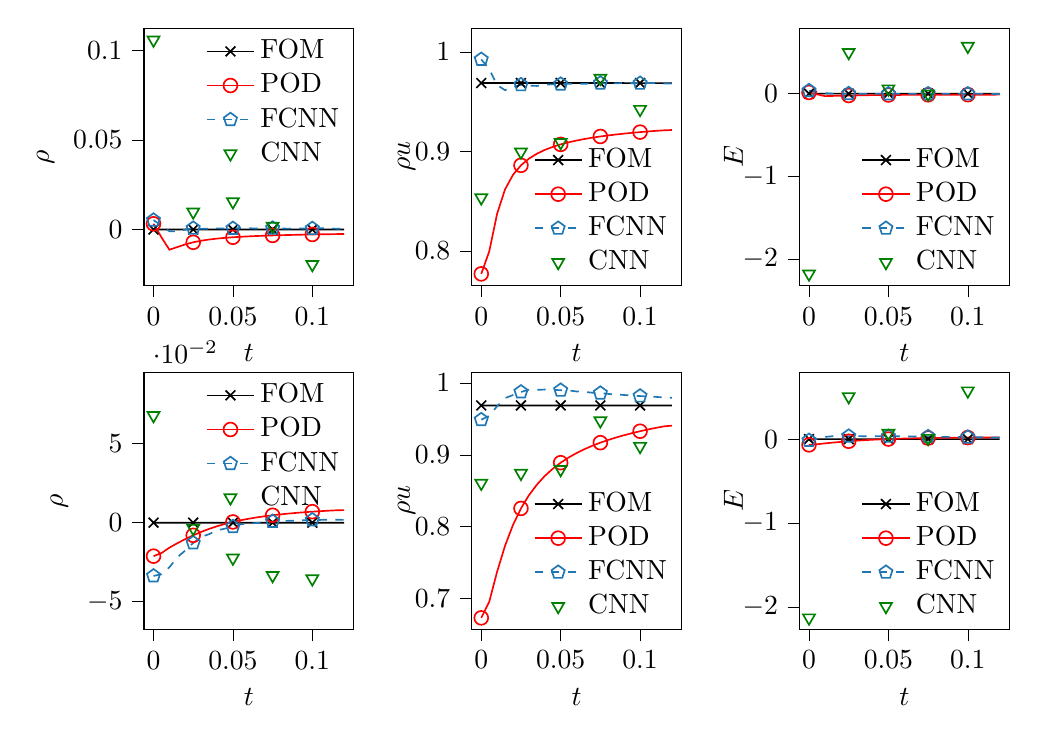
\begin{tikzpicture}

\definecolor{color0}{rgb}{0.12156862745098,0.466666666666667,0.705882352941177}

\begin{groupplot}[group style={group size=3 by 2,horizontal sep=1.5cm,vertical sep=1.1cm}]
\nextgroupplot[
legend cell align={left},
legend style={fill opacity=0,at={(1,1)},anchor=north east, draw opacity=1, text opacity=1, draw=none},
tick align=outside,
tick pos=left,
x grid style={white!69.0196078431373!black},
xlabel={\(t\)},
xmin=-0.006, xmax=0.126,
xtick style={color=black},
y grid style={white!69.0196078431373!black},
ylabel={\(\rho\)},
ymin=-0.031347233897592, ymax=0.112481710620415,
ytick style={color=black},
x tick label style={/pgf/number format/fixed},
y tick label style={/pgf/number format/fixed},
width=.35\textwidth,
height=.4\textwidth
]
\addplot [semithick, black, mark=x, mark size=2.5, mark repeat=5, mark options={solid}]
table {%
0 -1.02092058398284e-05
0.005 -1.00296277310008e-05
0.01 -1.00754774408074e-05
0.015 -9.94556989297735e-06
0.02 -9.88825775039004e-06
0.025 -9.78891667102744e-06
0.03 -9.50617667427878e-06
0.035 -8.79168510437012e-06
0.04 -8.65795674087622e-06
0.045 -8.76876023880868e-06
0.05 -7.97785246220428e-06
0.055 -7.50025113660513e-06
0.06 -8.10393920858132e-06
0.065 -7.41237249002324e-06
0.07 -7.04939547802041e-06
0.075 -7.61105464874845e-06
0.08 -6.77811794247418e-06
0.085 -6.39603687346835e-06
0.09 -6.72462659423445e-06
0.095 -6.48773634281952e-06
0.1 -5.78470718437529e-06
0.105 -6.13240095503897e-06
0.11 -6.53740687539539e-06
0.115 -4.7874756248234e-06
0.12 -2.92674087631895e-06
};
\addlegendentry{FOM}
\addplot [semithick, red, mark=o, mark size=2.5, mark repeat=5, mark options={solid}]
table {%
0 0.00320090038387377
0.005 -0.00437489518050427
0.01 -0.0113141287572276
0.015 -0.0098342336202677
0.02 -0.00832201483160588
0.025 -0.0071506711904874
0.03 -0.006269264595538
0.035 -0.00559929081244093
0.04 -0.00507985759631424
0.045 -0.00466825953316174
0.05 -0.00433514928440815
0.055 -0.00406028363599376
0.06 -0.00382951654002284
0.065 -0.00363279608841793
0.07 -0.00346284996611956
0.075 -0.00331432083461181
0.08 -0.00318319221832297
0.085 -0.00306640245018031
0.09 -0.00296158139310876
0.095 -0.00286686808712489
0.1 -0.00278078220517841
0.105 -0.00270213163336308
0.11 -0.0026299447166096
0.115 -0.00256341989258857
0.12 -0.0025314820932465
};
\addlegendentry{POD}
\addplot [semithick, color0, dashed, mark=pentagon, mark size=2.5, mark repeat=5, mark options={solid}]
table {%
0 0.00522449015618065
0.005 0.00223802796637784
0.01 -0.000970764085657549
0.015 -0.00110220367042047
0.02 -1.53349425886518e-05
0.025 0.000689030171201921
0.03 0.000360641294179231
0.035 0.00044592763656226
0.04 0.000652112245859371
0.045 0.000554050724865363
0.05 0.000587946806959394
0.055 0.00084763548026956
0.06 0.000720119091845106
0.065 0.000533394706543788
0.07 0.000645929577352433
0.075 0.000728898956324997
0.08 0.000566149202100519
0.085 0.000482535837463161
0.09 0.000636686499312589
0.095 0.000548915674862371
0.1 0.000538411848729936
0.105 0.000743403648712615
0.11 0.000605466238297936
0.115 0.000460749456230758
0.12 0.000461515469027063
};
\addlegendentry{FCNN}
\addplot [semithick, green!50!black, mark=triangle, mark size=2.5, mark repeat=5, mark options={solid,rotate=180}, only marks]
table {%
0 0.105944031324142
0.005 0.0516832065887911
0.01 -0.00857167136975079
0.015 -0.0144941722735368
0.02 0.00380830122874443
0.025 0.00983815544690003
0.03 0.00643285421224959
0.035 -0.00448056520559703
0.04 -0.0186044627275237
0.045 0.00790197497759948
0.05 0.0155578324428021
0.055 -0.00646213308359478
0.06 -0.00356465195998368
0.065 0.00381582822555515
0.07 -0.00903544899745157
0.075 0.0018757046797333
0.08 0.00199396640826421
0.085 -0.0120293368131712
0.09 0.00996308066905272
0.095 0.011515984168426
0.1 -0.0195331756885082
0.105 -0.00578945263838904
0.11 0.0182848977736825
0.115 -0.00607643371972699
0.12 -0.024809554601319
};
\addlegendentry{CNN}

\nextgroupplot[
legend cell align={left},
legend style={fill opacity=0,draw opacity=1, text opacity=1, at={(1,0)}, anchor=south east, draw=none},
tick align=outside,
tick pos=left,
x grid style={white!69.0196078431373!black},
xlabel={\(t\)},
xmin=-0.006, xmax=0.126,
xtick style={color=black},
y grid style={white!69.0196078431373!black},
ylabel={\(\rho u\)},
ymin=0.76497750084915, ymax=1.02392312637622,
ytick style={color=black},
x tick label style={/pgf/number format/fixed},
width=.35\textwidth,
height=.4\textwidth,
y label style={yshift=-.7em}
]
\addplot [semithick, black, mark=x, mark size=2.5, mark repeat=5, mark options={solid}]
table {%
0 0.968749501171195
0.005 0.968748980427641
0.01 0.968747985386072
0.015 0.968747021300463
0.02 0.968746000697791
0.025 0.968745012073585
0.03 0.968743993839396
0.035 0.968742949460326
0.04 0.968741950946862
0.045 0.96874097337124
0.05 0.968739957944206
0.055 0.968738944157029
0.06 0.968737963414923
0.065 0.968736944309001
0.07 0.96873587986985
0.075 0.96873495468575
0.08 0.968734019806657
0.085 0.968732920729255
0.09 0.968731860496209
0.095 0.968730922996592
0.1 0.968730020208966
0.105 0.96872891441061
0.11 0.968727923938824
0.115 0.968727045840522
0.12 0.968726553253322
};
\addlegendentry{FOM}
\addplot [semithick, red, mark=o, mark size=2.5, mark repeat=5, mark options={solid}]
table {%
0 0.776747756554926
0.005 0.79922955089991
0.01 0.837353952897857
0.015 0.861900926991852
0.02 0.876455591781436
0.025 0.885983575566024
0.03 0.892681148197205
0.035 0.897645437682196
0.04 0.901479314467375
0.045 0.904538276949287
0.05 0.907043868523403
0.055 0.909140543750316
0.06 0.910926152329419
0.065 0.912469183248853
0.07 0.913818965136114
0.075 0.915011933164954
0.08 0.916075607301774
0.085 0.917031190999539
0.09 0.91789531243126
0.095 0.918681218375196
0.1 0.919399610528167
0.105 0.9200592433798
0.11 0.920667359928453
0.115 0.921230014745539
0.12 0.921500667907083
};
\addlegendentry{POD}
\addplot [semithick, color0, dashed, mark=pentagon, mark size=2.5, mark repeat=5, mark options={solid}]
table {%
0 0.99255735321579
0.005 0.98291644572423
0.01 0.966706887232892
0.015 0.961570447754117
0.02 0.964582067033194
0.025 0.967063569879548
0.03 0.966240846068845
0.035 0.965833740203562
0.04 0.967266327789681
0.045 0.967439440894019
0.05 0.967625114469151
0.055 0.967984018237485
0.06 0.968042696106084
0.065 0.96798582029462
0.07 0.968520641452426
0.075 0.968677012288404
0.08 0.968224639722065
0.085 0.96852887747289
0.09 0.968850592860337
0.095 0.968569526840721
0.1 0.968508102611457
0.105 0.968882985863736
0.11 0.968749204483361
0.115 0.968243563801837
0.12 0.968199305635565
};
\addlegendentry{FCNN}
\addplot [semithick, green!50!black, mark=triangle, mark size=2.5, mark repeat=5, mark options={solid,rotate=180}, only marks]
table {%
0 0.853358098260489
0.005 0.887302798525615
0.01 0.946574235275696
0.015 0.97026433532651
0.02 0.929223370446957
0.025 0.899488979637141
0.03 0.941904080796699
0.035 0.948295325839591
0.04 0.969445355819724
0.045 0.96948865363312
0.05 0.90897449561884
0.055 0.958882224284184
0.06 1.01215287067045
0.065 0.938565923528354
0.07 0.91992112784801
0.075 0.973712211065665
0.08 0.94272326490316
0.085 0.929348146634882
0.09 0.96821875316828
0.095 0.961927331827917
0.1 0.942337237367418
0.105 0.881994380596876
0.11 0.976709562654605
0.115 0.980358973725224
0.12 0.829531761849992
};
\addlegendentry{CNN}

\nextgroupplot[
legend cell align={left},
legend style={fill opacity=0,draw opacity=1, text opacity=1, at={(1,0)}, anchor=south east, draw=none},
tick align=outside,
tick pos=left,
x grid style={white!69.0196078431373!black},
xlabel={\(t\)},
xmin=-0.006, xmax=0.126,
xtick style={color=black},
y grid style={white!69.0196078431373!black},
ylabel={\(E\)},
ymin=-2.31850155192636, ymax=0.790251347012884,
ytick style={color=black},
x tick label style={/pgf/number format/fixed},
width=.35\textwidth,
height=.4\textwidth,
y label style={yshift=-.7em}
]
\addplot [semithick, black, mark=x, mark size=2.5, mark repeat=5, mark options={solid}]
table {%
0 4.87866297049777e-05
0.005 4.80259367172664e-05
0.01 4.65949778458707e-05
0.015 4.54067031263605e-05
0.02 4.42829340876472e-05
0.025 4.31550719284246e-05
0.03 4.21234150600469e-05
0.035 4.10590815498324e-05
0.04 4.00091049534979e-05
0.045 3.90511888817002e-05
0.05 3.80374836694841e-05
0.055 3.7035708462696e-05
0.06 3.60308381281982e-05
0.065 3.50356377083472e-05
0.07 3.40427852520975e-05
0.075 3.30760824311938e-05
0.08 3.21252078379075e-05
0.085 3.11066398879234e-05
0.09 3.01230652937079e-05
0.095 2.91512564523089e-05
0.1 2.82270395430828e-05
0.105 2.72673938148671e-05
0.11 2.6235596106261e-05
0.115 2.52928882495951e-05
0.12 2.48756531604499e-05
};
\addlegendentry{FOM}
\addplot [semithick, red, mark=o, mark size=2.5, mark repeat=5, mark options={solid}]
table {%
0 0.0143189699659771
0.005 -0.00810455144663891
0.01 -0.0298314957712229
0.015 -0.0275728370352653
0.02 -0.024684948257427
0.025 -0.022325029227499
0.03 -0.0204887750834786
0.035 -0.019056989877587
0.04 -0.0179250310035748
0.045 -0.0170152913195345
0.05 -0.0162722243644673
0.055 -0.0156561085564633
0.06 -0.0151382260786583
0.065 -0.014697505192796
0.07 -0.0143182442505783
0.075 -0.0139885691535824
0.08 -0.0136993768651301
0.085 -0.0134436013260313
0.09 -0.013215695412427
0.095 -0.013011259464129
0.1 -0.0128267704325289
0.105 -0.012659380999672
0.11 -0.0125067683163103
0.115 -0.0123670190485541
0.12 -0.0123001435898757
};
\addlegendentry{POD}
\addplot [semithick, color0, dashed, mark=pentagon, mark size=2.5, mark repeat=5, mark options={solid}]
table {%
0 0.0360973720480686
0.005 0.0229009781790843
0.01 0.00583964003358162
0.015 -0.000117786223665206
0.02 -5.73832530541551e-05
0.025 0.00018579220459003
0.03 -0.00244610390549838
0.035 -0.00274824485896374
0.04 -0.00206376247841789
0.045 -0.00240319216478113
0.05 -0.00277106366328894
0.055 -0.00236928252206425
0.06 -0.00246256101745601
0.065 -0.00307336741648001
0.07 -0.00275752749475799
0.075 -0.00264167383333458
0.08 -0.00339416363136991
0.085 -0.00300615922562031
0.09 -0.00258383118143257
0.095 -0.00314659748762125
0.1 -0.00314209016637079
0.105 -0.00266266636015189
0.11 -0.00268276351402719
0.115 -0.00353034803091745
0.12 -0.00427924698373516
};
\addlegendentry{FCNN}
\addplot [semithick, green!50!black, mark=triangle, mark size=2.5, mark repeat=5, mark options={solid,rotate=180}, only marks]
table {%
0 -2.17719460197458
0.005 -1.20071149218471
0.01 -0.152507668712161
0.015 -0.335833045789045
0.02 0.648944397061101
0.025 0.498273199221543
0.03 -0.681839756482006
0.035 0.176069682927949
0.04 0.193472237641728
0.045 -0.430439559572847
0.05 0.0584560612445699
0.055 0.257541708034378
0.06 -0.301384298495798
0.065 0.0215179014772033
0.07 0.462341463778831
0.075 -0.00350134009975278
0.08 -0.171256620657246
0.085 0.148787423086613
0.09 -0.107412166454019
0.095 -0.372344121075709
0.1 0.572956203903821
0.105 0.563652518126105
0.11 -0.510284719394772
0.115 -0.307766960783653
0.12 0.184716161842637
};
\addlegendentry{CNN}

\nextgroupplot[
legend cell align={left},
legend style={fill opacity=0, text opacity=1, at={(1,1)}, anchor=north east, draw=none},
tick align=outside,
tick pos=left,
x grid style={white!69.0196078431373!black},
xlabel={\(t\)},
xmin=-0.006, xmax=0.126,
xtick style={color=black},
y grid style={white!69.0196078431373!black},
ylabel={\(\rho\)},
ymin=-0.0676974161618712, ymax=0.0952766411274003,
ytick style={color=black},
x tick label style={/pgf/number format/fixed},
width=.35\textwidth,
height=.4\textwidth
]
\addplot [semithick, black, mark=x, mark size=2.5, mark repeat=5, mark options={solid}]
table {%
0 1.75757278952915e-07
0.005 1.91040520292063e-07
0.01 2.63635932640227e-07
0.015 1.49011604833049e-07
0.02 -3.01844046646238e-07
0.025 2.71277556862515e-07
0.03 3.66797813455833e-07
0.035 -1.22265944924038e-07
0.04 5.272718510696e-07
0.045 -5.34913482397315e-08
0.05 -6.03688071976194e-07
0.055 3.24768897996819e-07
0.06 5.88404823531619e-07
0.065 2.29248584560082e-08
0.07 -1.56653229055337e-07
0.075 9.93410722571753e-08
0.08 -1.79578094616772e-07
0.085 -9.59023445545881e-07
0.09 -5.08167801172021e-07
0.095 -1.66969421400154e-06
0.1 -4.5200188978356e-06
0.105 -8.4860202633763e-06
0.11 -1.75222372433836e-05
0.115 -3.26373638230848e-05
0.12 -4.18225924079252e-05
};
\addlegendentry{FOM}
\addplot [semithick, red, mark=o, mark size=2.5, mark repeat=5, mark options={solid}]
table {%
0 -0.0212029747826676
0.005 -0.0192443298188607
0.01 -0.0158249458355471
0.015 -0.013006378137753
0.02 -0.010391648459219
0.025 -0.00799430478169683
0.03 -0.0058375091076357
0.035 -0.00392724004669986
0.04 -0.00225379066242226
0.045 -0.000797663730928377
0.05 0.000465209834587199
0.055 0.00155988199323787
0.06 0.00251024276713707
0.065 0.00333791211889434
0.07 0.00406180221506247
0.075 0.00469807848833881
0.08 0.00526033382170255
0.085 0.00575985393346912
0.09 0.00620589623488144
0.095 0.00660593582998814
0.1 0.00696585660401894
0.105 0.00729008480776372
0.11 0.00758167704933754
0.115 0.00784238327669584
0.12 0.0079651537237595
};
\addlegendentry{POD}
\addplot [semithick, color0, dashed, mark=pentagon, mark size=2.5, mark repeat=5, mark options={solid}]
table {%
0 -0.0337256205817482
0.005 -0.0326607484394259
0.01 -0.0282118052769533
0.015 -0.0219212716015562
0.02 -0.0176159442903767
0.025 -0.0128136095232634
0.03 -0.00905398715239158
0.035 -0.00726883013088298
0.04 -0.00484687592595634
0.045 -0.0037650649364096
0.05 -0.00254844983992086
0.055 -0.00100207138950026
0.06 -0.000493180138093408
0.065 -0.000213338778564776
0.07 0.000264983839144861
0.075 0.000794312785352247
0.08 0.00102030531240871
0.085 0.0011805769724802
0.09 0.00131457058999018
0.095 0.00161062185770788
0.1 0.00175724253775655
0.105 0.00173451832663574
0.11 0.00191565244816871
0.115 0.00184704746620667
0.12 0.00176488159175392
};
\addlegendentry{FCNN}
\addplot [semithick, green!50!black, mark=triangle, mark size=2.5, mark repeat=5, mark options={solid,rotate=180}, only marks]
table {%
0 0.0678687294324334
0.005 0.0279934780719913
0.01 -0.0271384150554042
0.015 -0.0346271349833529
0.02 -0.00848802618490652
0.025 -0.00355549729787441
0.03 -0.021275022091011
0.035 -0.0292548995751645
0.04 -0.0393498173126829
0.045 -0.0362662665354847
0.05 -0.0223790300198061
0.055 -0.0234647630116882
0.06 -0.0167072124970247
0.065 -0.0117229536557772
0.07 -0.0384964889440838
0.075 -0.0334069896967009
0.08 -0.0258152645367886
0.085 -0.0298783374138338
0.09 -0.0244208406179425
0.095 -0.0231431577450181
0.1 -0.0355150760748373
0.105 -0.0475942247953185
0.11 -0.00332274498084217
0.115 -0.0241975791943432
0.12 -0.0802895044669043
};
\addlegendentry{CNN}

\nextgroupplot[
legend cell align={left},
legend style={fill opacity=0,text opacity=1, at={(1,0)}, anchor=south east, draw=none},
tick align=outside,
tick pos=left,
x grid style={white!69.0196078431373!black},
xlabel={\(t\)},
xmin=-0.006, xmax=0.126,
xtick style={color=black},
y grid style={white!69.0196078431373!black},
ylabel={\(\rho u\)},
ymin=0.656514441384938, ymax=1.0150522738195,
ytick style={color=black},
x tick label style={/pgf/number format/fixed},
width=.35\textwidth,
height=.4\textwidth,
y label style={yshift=-.7em}
]
\addplot [semithick, black, mark=x, mark size=2.5, mark repeat=5, mark options={solid}]
table {%
0 0.968749926582301
0.005 0.968749966029677
0.01 0.968750028467607
0.015 0.968749982144151
0.02 0.968749954959954
0.025 0.968749994054567
0.03 0.96874992314994
0.035 0.968749928522076
0.04 0.968750036693629
0.045 0.968749961528333
0.05 0.96874993946036
0.055 0.968750028431101
0.06 0.968750025404645
0.065 0.968749964363327
0.07 0.968749897481958
0.075 0.968749819771261
0.08 0.96874967320004
0.085 0.968748914638772
0.09 0.968746788729474
0.095 0.968741946861179
0.1 0.968731876128718
0.105 0.968712914797148
0.11 0.968679924855179
0.115 0.968626307013933
0.12 0.968593392665735
};
\addlegendentry{FOM}
\addplot [semithick, red, mark=o, mark size=2.5, mark repeat=5, mark options={solid}]
table {%
0 0.672811615586509
0.005 0.695017748286703
0.01 0.73727280043653
0.015 0.773446350407561
0.02 0.802344052034812
0.025 0.825274622257849
0.03 0.843591013419188
0.035 0.858386241114922
0.04 0.870494322508944
0.045 0.880540271925342
0.05 0.88899027168719
0.055 0.896192447350749
0.06 0.902407886411629
0.065 0.907833617723927
0.07 0.912619446342193
0.075 0.916880236020742
0.08 0.920704862641226
0.085 0.924162740697142
0.09 0.927308574315828
0.095 0.930185800458824
0.1 0.932829064067617
0.105 0.935265979427903
0.11 0.937518374970946
0.115 0.939603177413559
0.12 0.940605512911738
};
\addlegendentry{POD}
\addplot [semithick, color0, dashed, mark=pentagon, mark size=2.5, mark repeat=5, mark options={solid}]
table {%
0 0.948846632342866
0.005 0.954152703242968
0.01 0.967721876710957
0.015 0.978894484640245
0.02 0.983309222815127
0.025 0.987517708186292
0.03 0.990693046549735
0.035 0.990407735986156
0.04 0.990899470677622
0.045 0.990649431277702
0.05 0.989912680358204
0.055 0.989661670417294
0.06 0.988217143517631
0.065 0.987550813672889
0.07 0.986486527349929
0.075 0.985869276337326
0.08 0.984799591665212
0.085 0.983933408491749
0.09 0.983336423052245
0.095 0.982431453860253
0.1 0.981841696365656
0.105 0.981093008673698
0.11 0.980674354561568
0.115 0.979852107387796
0.12 0.979396904758094
};
\addlegendentry{FCNN}
\addplot [semithick, green!50!black, mark=triangle, mark size=2.5, mark repeat=5, mark options={solid,rotate=180}, only marks]
table {%
0 0.860473237123076
0.005 0.885082150192434
0.01 0.928426369986636
0.015 0.945950995161388
0.02 0.904390544953354
0.025 0.874297395343156
0.03 0.919500090265407
0.035 0.924854385510232
0.04 0.944966989635446
0.045 0.945220332597675
0.05 0.879612664571825
0.055 0.934335838481422
0.06 0.998755099617925
0.065 0.917349259203859
0.07 0.886255976842381
0.075 0.947432327189556
0.08 0.917552957599429
0.085 0.897157233189265
0.09 0.941230996731097
0.095 0.938804230153156
0.1 0.911739614725017
0.105 0.843112473926192
0.11 0.960578430300417
0.115 0.959220679106179
0.12 0.779141892528088
};
\addlegendentry{CNN}

\nextgroupplot[
legend cell align={left},
legend style={fill opacity=0, text opacity=1, at={(1,0)}, anchor=south east, draw=none},
tick align=outside,
tick pos=left,
x grid style={white!69.0196078431373!black},
xlabel={\(t\)},
xmin=-0.006, xmax=0.126,
xtick style={color=black},
y grid style={white!69.0196078431373!black},
ylabel={\(E\)},
ymin=-2.2693476394536, ymax=0.797403375676948,
ytick style={color=black},
x tick label style={/pgf/number format/fixed},
width=.35\textwidth,
height=.4\textwidth,
y label style={yshift=-.7em}
]
\addplot [semithick, black, mark=x, mark size=2.5, mark repeat=5, mark options={solid}]
table {%
0 5.27370929148674e-08
0.005 8.80836772410021e-08
0.01 8.63330598122047e-08
0.015 1.53081778364594e-08
0.02 4.93576379767546e-08
0.025 6.90528523250578e-08
0.03 1.84607920061808e-08
0.035 5.72133309617584e-08
0.04 5.6898358025137e-08
0.045 3.65553809444918e-08
0.05 2.28335146346126e-08
0.055 3.60124658982386e-08
0.06 1.03884925550801e-07
0.065 4.81812278962934e-08
0.07 -5.01372383610033e-08
0.075 -1.72955385124851e-07
0.08 -7.10039881113289e-07
0.085 -2.53672278560657e-06
0.09 -6.94816306889834e-06
0.095 -1.67507910759923e-05
0.1 -3.62984502366714e-05
0.105 -7.15032817026895e-05
0.11 -0.000130049924880637
0.115 -0.000220557168169933
0.12 -0.000274955867070048
};
\addlegendentry{FOM}
\addplot [semithick, red, mark=o, mark size=2.5, mark repeat=5, mark options={solid}]
table {%
0 -0.0682411789316859
0.005 -0.0618224505428948
0.01 -0.050574594990529
0.015 -0.0413276928304036
0.02 -0.032871351735313
0.025 -0.0252074283347348
0.03 -0.0183846310619558
0.035 -0.0124059827567464
0.04 -0.00722961285070056
0.045 -0.00278548101118403
0.05 0.00100924423666271
0.055 0.00423951236771458
0.06 0.00698599559464697
0.065 0.00932178558594998
0.07 0.0113110963351915
0.075 0.0130091647361823
0.08 0.0144627958275194
0.085 0.0157111905574006
0.09 0.0167868277041805
0.095 0.0177162678121405
0.1 0.0185208209987948
0.105 0.019217077294428
0.11 0.0198173363775211
0.115 0.0203299918936466
0.12 0.0205652356026462
};
\addlegendentry{POD}
\addplot [semithick, color0, dashed, mark=pentagon, mark size=2.5, mark repeat=5, mark options={solid}]
table {%
0 -0.0151793320639584
0.005 0.00053994949383096
0.01 0.0262932544727548
0.015 0.0349235767703533
0.02 0.0333795951271085
0.025 0.0350968105173024
0.03 0.0355935866259003
0.035 0.034886039685162
0.04 0.0353222983526926
0.045 0.0341312459297924
0.05 0.033947001761085
0.055 0.0337190867195183
0.06 0.0325485077185341
0.065 0.0315345865527412
0.07 0.0302826758071149
0.075 0.0291376590175219
0.08 0.0277780434455401
0.085 0.0268394665786609
0.09 0.0257280005792246
0.095 0.024633435005704
0.1 0.0234614136883806
0.105 0.0223044056672919
0.11 0.0212615342017344
0.115 0.0201121194293279
0.12 0.0197042712382327
};
\addlegendentry{FCNN}
\addplot [semithick, green!50!black, mark=triangle, mark size=2.5, mark repeat=5, mark options={solid,rotate=180}, only marks]
table {%
0 -2.12994986603857
0.005 -1.16855299577587
0.01 -0.14149678977406
0.015 -0.328904931456748
0.02 0.658005602261923
0.025 0.507371738388851
0.03 -0.667596592072631
0.035 0.189154708770655
0.04 0.203141442897838
0.045 -0.413931727116317
0.05 0.0700945391622199
0.055 0.26894278849737
0.06 -0.276267618522503
0.065 0.0385397221438666
0.07 0.465582343235745
0.075 0.00934939013428249
0.08 -0.156551761117125
0.085 0.150756091889352
0.09 -0.0948361626110241
0.095 -0.354554159531791
0.1 0.575086976019694
0.105 0.567620995507102
0.11 -0.487382764747942
0.115 -0.29382469498087
0.12 0.178325289514078
};
\addlegendentry{CNN}
\end{groupplot}

\end{tikzpicture}
}
					\caption{
						Conservation properties of $f$ and $\tilde{f}$, $\mathbf{H}$ top and $\mathbf{R}$ bottom.}
				\end{figure}
			\end{column}
		\begin{column}{.39\textwidth}
			\begin{itemize}
				\item\emph{POD}:
				\begin{itemize}
					\item $\mathbf{H}$ \& $\mathbf{R}$ \colorbox{red}{- mass} 
					\& \colorbox{ProcessBlue}{+ mass}
					\item $\mathbf{H}$ \& $\mathbf{R}$ \colorbox{ProcessBlue}{+++ momentum}
					\item $\mathbf{H}$ \& $\mathbf{R}$ \colorbox{green}{energy} 
				\end{itemize}
				\item\emph{FCNN}:
				\begin{itemize}
					\item $\mathbf{H}$ \& $\mathbf{R}$ \colorbox{green}{mass} 
					\item $\mathbf{H}$ \& $\mathbf{R}$ \colorbox{red}{- momentum} 
					\& \colorbox{ProcessBlue}{+ momentum}
					\item $\mathbf{H}$ \& $\mathbf{R}$ \colorbox{green}{energy} 
				\end{itemize}
				\item\emph{CNN}:
				\begin{itemize}
					\item No conservation
				\end{itemize}
			\end{itemize}
		\end{column}
	\end{columns}
\end{frame}
\begin{frame}[fragile]{Interpretabiliy}
			\begin{columns}
		\begin{column}{.65\textwidth}
			\begin{figure}
				\only<1>{\scalebox{.7}[.7]{\input{Figures/heat_hy.tex}}
					\caption{Pearson correlation between of macroscopic quantities and intrinsic variables for $\mathbf{H}$}}
				\only<2>{\scalebox{.7}[.7]{\input{Figures/heat_rare.tex}}
					\caption{Pearson correlation between of macroscopic quantities and intrinsic variables for $\mathbf{R}$}}
			\end{figure}
		\end{column}
		\begin{column}{.35\textwidth}
			\begin{itemize}
				\item\emph{1}:
				\begin{itemize}
					\only<1>{\item $E$: $0.98$ \& $\rho$: $0.97$}
					\only<2>{\item $u$: $-0.92$ \& $\rho u$: $-0.85$} 
				\end{itemize}
				\item\emph{2}:
				\begin{itemize}
					\only<1>{\item $u$: $-0.75$ \& $\rho$: $0.71$}
					\only<2>{\item $\rho$: $-0.8$ \& $E$: $-0.74$}
				\end{itemize}
				\item\emph{3}:
				\begin{itemize}
					\only<1>{\item $\rho u$: $0.69$ \& $T$: $-0.54$}
					\only<2>{\item $\rho$: $0.49$ \& $\rho u$: $0.49$}
				\end{itemize}
				\only<2>{\item\emph{4}:
				\begin{itemize}
					\item $\rho$: $1$ \& $E$: $0.96$
				\end{itemize}}
				\only<2>{\item\emph{5}:
				\begin{itemize}
					\item $\rho$: $-0.89$ \& $T$: $-0.89$
				\end{itemize}}
			\end{itemize}
		\end{column}
	\end{columns}
\end{frame}
\begin{frame}[fragile]{Interpolation}
	\begin{table}[H]
		\vspace{-2em}
		\footnotesize
		\centering
		\vspace{.5em}
		\caption{Validation and metric results for the interpolation task with 13, 9, 7 and 5 time steps.}
		\begin{tabular*}{11cm}{ @{\extracolsep{\fill}} c c c c c c c c @{} }
			\toprule
			$n$& \(\Delta t^*\) & \multicolumn{2}{c}{Validation error} & \multicolumn{2}{c}{\(L_2\)-error}& \multicolumn{2}{c}{$L_2$-error} \\ [.5ex]
			& & \(\mathbf{H}^*\)&\(\mathbf{R}^*\)&\(\mathbf{H}^*\)&\(\mathbf{R}^*\)&\(\tilde{\mathbf{H}}^*\)&\(\tilde{\mathbf{R}}^*\)\\   
			\hline
			13& 0.01s   & \num{2.5e-8} & \num{2.9e-7} & 0.0018 & 0.0054 & 0.0036 & 0.0058 \\
			9& 	0.015s	& \num{2.9e-8} & \num{9.5e-8} & 0.0017 & 0.0038 & 0.0067 & 0.0056 \\
			7&  0.02s 	& \num{2.5e-8} & \num{1.6e-7} & 0.0019 & 0.0042 & 0.0101 & 0.0073\\
			5&  0.025s  & \num{1.7e-7} & \num{1.6e-7} & 0.0039 & 0.0051 & 0.0367 & 0.0138\\
			\bottomrule
		\end{tabular*}
	\end{table}
	\begin{figure}
		\scalebox{.7}[.7]{% This file was created by tikzplotlib v0.9.8.
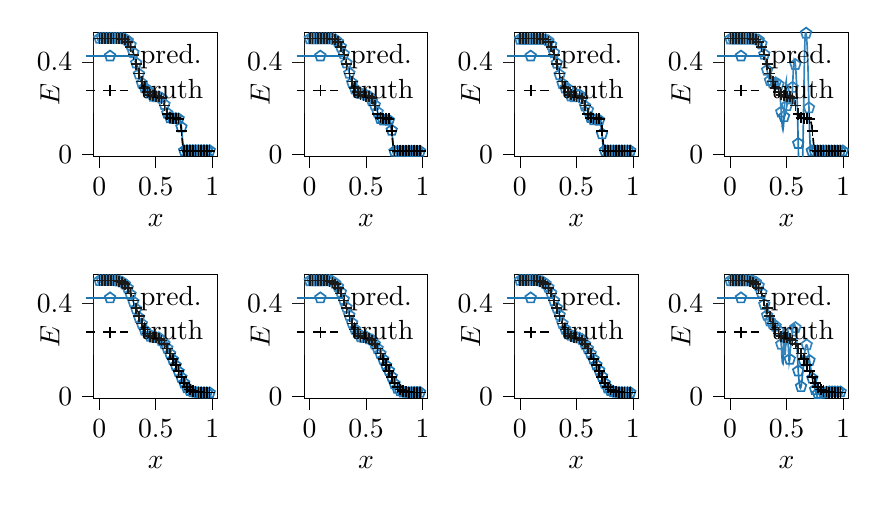
\begin{tikzpicture}

%\definecolor{color0}{rgb}{0.12156862745098,0.466666666666667,0.705882352941177}

\begin{groupplot}[
group style={group size=4 by 2,
	horizontal sep= 1.1cm,
	vertical sep = 1.5cm},
legend cell align={left},
legend style={fill opacity=0.1, draw opacity=1, text opacity=1, at={(1,1)}, anchor=north east, draw=none},
tick align=outside,
tick pos=left,
x grid style={white!69.0196078431373!black},
xtick style={color=black},
xmin=-0.04725, xmax=1.04725,
y grid style={white!69.0196078431373!black},
ytick style={color=black},
ymin=-0.00862946381914901, ymax=0.525234224104059,
height=.26\textwidth,
width=.26\textwidth,
ytick={0.4,0.0},
y label style={yshift=-1.5em},
ylabel={\(E\)},
xlabel={\(x\)}
]
\nextgroupplot[
]
\addplot [semithick, color0, mark=pentagon, mark size=2, mark options={solid}, mark repeat=5]
table {%
0.0025 0.500966441400048
0.0075 0.500966441400048
0.0125 0.500966441400048
0.0175 0.500966441400048
0.0225 0.500966441400048
0.0275 0.500966441400048
0.0325 0.500966441400048
0.0375 0.500966441400048
0.0425 0.500966441400048
0.0475 0.500966441400048
0.0525 0.500966441400048
0.0575 0.500966441400048
0.0625 0.500966441400048
0.0675 0.500966441400048
0.0725 0.500966441400048
0.0775 0.500966441400048
0.0825 0.500967692834822
0.0875 0.500967692834822
0.0925 0.500967692834822
0.0975 0.500967692834822
0.1025 0.500966441400048
0.1075 0.500966441400048
0.1125 0.500967597754165
0.1175 0.500965941786993
0.1225 0.500964944382111
0.1275 0.500965247679358
0.1325 0.500964103414426
0.1375 0.500964707496881
0.1425 0.500962536593219
0.1475 0.500962675383346
0.1525 0.500958562391327
0.1575 0.50095609745356
0.1625 0.500948389765865
0.1675 0.50093985841215
0.1725 0.500922775357207
0.1775 0.500898598493976
0.1825 0.500861689112459
0.1875 0.500806615431834
0.1925 0.500729709624702
0.1975 0.500613877049344
0.2025 0.500453236081643
0.2075 0.500228935034558
0.2125 0.499922009901528
0.2175 0.499505351139985
0.2225 0.498957466156828
0.2275 0.49824097054406
0.2325 0.497319237712898
0.2375 0.496155300253737
0.2425 0.494702834230014
0.2475 0.492916208556779
0.2525 0.490747586485089
0.2575 0.488154722592673
0.2625 0.485080988309879
0.2675 0.481485550953481
0.2725 0.477324330057087
0.2775 0.472550738705105
0.2825 0.467126725574723
0.2875 0.461017653391835
0.2925 0.454254825641467
0.2975 0.446959481873421
0.3025 0.43917348762695
0.3075 0.430933249436266
0.3125 0.422290634647468
0.3175 0.413304421601343
0.3225 0.404033398969436
0.3275 0.394550400356085
0.3325 0.384930248272103
0.3375 0.375253406167731
0.3425 0.365603274223205
0.3475 0.356070781072511
0.3525 0.346741047924856
0.3575 0.337749157420542
0.3625 0.32921535371412
0.3675 0.321251493891637
0.3725 0.313962094360267
0.3775 0.30745282712769
0.3825 0.301826230810379
0.3875 0.297179625735849
0.3925 0.293602919363042
0.3975 0.290726977558576
0.4025 0.287929685575362
0.4075 0.285315715472761
0.4125 0.282903945691024
0.4175 0.28070451224265
0.4225 0.278718658021485
0.4275 0.276941216172562
0.4325 0.275189702925511
0.4375 0.273215587789909
0.4425 0.271021709761754
0.4475 0.267980871517886
0.4525 0.264518928094448
0.4575 0.260964494922855
0.4625 0.257609464556163
0.4675 0.254689543496908
0.4725 0.252407509246045
0.4775 0.250855547899266
0.4825 0.249946263094105
0.4875 0.249510182114481
0.4925 0.249353294375636
0.4975 0.249320562922332
0.5025 0.249309810651839
0.5075 0.249282308985953
0.5125 0.249221236533866
0.5175 0.249120555012498
0.5225 0.248964621306621
0.5275 0.248723098006261
0.5325 0.248333655713773
0.5375 0.247712631442593
0.5425 0.246732817149372
0.5475 0.245234903725664
0.5525 0.24299851881913
0.5575 0.239798197374699
0.5625 0.23545103981683
0.5675 0.229876133589901
0.5725 0.223150389273916
0.5775 0.21564424712097
0.5825 0.207748240692319
0.5875 0.199842282885996
0.5925 0.192070842801771
0.5975 0.184724939070208
0.6025 0.178062210268081
0.6075 0.172267064520696
0.6125 0.167448406476014
0.6175 0.163616007241544
0.6225 0.160696287357321
0.6275 0.158569520195823
0.6325 0.157090036366039
0.6375 0.156113371815827
0.6425 0.155512548337659
0.6475 0.155180090076116
0.6525 0.155026719874116
0.6575 0.154993904801331
0.6625 0.155030481997158
0.6675 0.155105266230784
0.6725 0.155192550587733
0.6775 0.155269683812849
0.6825 0.155306362997438
0.6875 0.155272136111922
0.6925 0.155094246090636
0.6975 0.154664342009552
0.7025 0.153787732030852
0.7075 0.152122109446096
0.7125 0.149056741334787
0.7175 0.143534046524728
0.7225 0.133946573565147
0.7275 0.117838136316971
0.7325 0.0925208064022269
0.7375 0.0591227234284908
0.7425 0.0293261799451487
0.7475 0.0168003882274276
0.7525 0.0157240875249655
0.7575 0.0163573134421958
0.7625 0.0166573713214081
0.7675 0.0167494297996553
0.7725 0.0167748245069967
0.7775 0.0167818115536505
0.7825 0.0167826040075922
0.7875 0.016784948697217
0.7925 0.0167852624665245
0.7975 0.0167846713210671
0.8025 0.0167833686407078
0.8075 0.0167833624862135
0.8125 0.0167833624862135
0.8175 0.0167833624862135
0.8225 0.0167833624862135
0.8275 0.0167833624862135
0.8325 0.0167833624862135
0.8375 0.0167833624862135
0.8425 0.0167833624862135
0.8475 0.0167833624862135
0.8525 0.0167833624862135
0.8575 0.0167833624862135
0.8625 0.0167833624862135
0.8675 0.0167833624862135
0.8725 0.0167833624862135
0.8775 0.0167833624862135
0.8825 0.0167833624862135
0.8875 0.0167833624862135
0.8925 0.0167833624862135
0.8975 0.0167833624862135
0.9025 0.0167833624862135
0.9075 0.0167833624862135
0.9125 0.0167833624862135
0.9175 0.0167833624862135
0.9225 0.0167833624862135
0.9275 0.0167833624862135
0.9325 0.0167833624862135
0.9375 0.0167833624862135
0.9425 0.0167833624862135
0.9475 0.0167833624862135
0.9525 0.0167833624862135
0.9575 0.0167833624862135
0.9625 0.0167833624862135
0.9675 0.0167833624862135
0.9725 0.0167833624862135
0.9775 0.0167833624862135
0.9825 0.0167833624862135
0.9875 0.0167833624862135
0.9925 0.0167830305595778
0.9975 0.0167830305595778
};
\addlegendentry{pred.}
\addplot [semithick, black, mark=+, mark size=2, mark options={solid},
dashed,mark repeat=5]
table {%
0.0025 0.499999997249975
0.0075 0.499999997249952
0.0125 0.49999999724991
0.0175 0.49999999724983
0.0225 0.499999997249673
0.0275 0.499999997249343
0.0325 0.499999997248633
0.0375 0.499999997247108
0.0425 0.499999997243849
0.0475 0.499999997236918
0.0525 0.49999999722231
0.0575 0.499999997191854
0.0625 0.499999997129034
0.0675 0.499999997000896
0.0725 0.499999996742452
0.0775 0.499999996227163
0.0825 0.499999995211631
0.0875 0.499999993233655
0.0925 0.499999989426775
0.0975 0.499999982187882
0.1025 0.499999968590229
0.1075 0.499999943362711
0.1125 0.49999989714242
0.1175 0.499999813531151
0.1225 0.499999664219035
0.1275 0.499999401043895
0.1325 0.499998943288962
0.1375 0.499998157735899
0.1425 0.499996827939107
0.1475 0.499994607841606
0.1525 0.499990953221392
0.1575 0.499985022618125
0.1625 0.499975537529369
0.1675 0.499960590121808
0.1725 0.499937386002681
0.1775 0.499901910468537
0.1825 0.499848509989294
0.1875 0.499769387444734
0.1925 0.499654020597409
0.1975 0.499488528760043
0.2025 0.499255032002629
0.2075 0.498931068658278
0.2125 0.498489156918177
0.2175 0.497896600156329
0.2225 0.497115637784343
0.2275 0.496104028964957
0.2325 0.494816122733982
0.2375 0.493204416224345
0.2425 0.491221538805241
0.2475 0.488822534483274
0.2525 0.48596726066466
0.2575 0.482622690300756
0.2625 0.478764904226945
0.2675 0.474380592224794
0.2725 0.469467939022164
0.2775 0.46403684380784
0.2825 0.458108495428486
0.2875 0.451714388097888
0.2925 0.444894905918178
0.2975 0.437697625542276
0.3025 0.430175486289908
0.3075 0.422384960603958
0.3125 0.414384331017942
0.3175 0.406232148833711
0.3225 0.397985919383409
0.3275 0.389701032374154
0.3325 0.381429935098179
0.3375 0.373221531647741
0.3425 0.365120782228682
0.3475 0.357168472254166
0.3525 0.349401119983176
0.3575 0.341850992947928
0.3625 0.334546206351425
0.3675 0.327510880277021
0.3725 0.320765336408751
0.3775 0.314326318665062
0.3825 0.308207225493483
0.3875 0.302418344457086
0.3925 0.296967082133645
0.3975 0.291858184256781
0.4025 0.287093942489105
0.4075 0.28267438527183
0.4125 0.278597450881622
0.4175 0.27485914117029
0.4225 0.271453654478241
0.4275 0.268373495894285
0.4325 0.265609562373013
0.4375 0.263151199234399
0.4425 0.260986223393296
0.4475 0.25910090775627
0.4525 0.257479921790285
0.4575 0.256106228028066
0.4625 0.254960948347607
0.4675 0.254023244450158
0.4725 0.253270307401023
0.4775 0.252677601550096
0.4825 0.252219485718782
0.4875 0.251870132202037
0.4925 0.251604330194165
0.4975 0.251397729084703
0.5025 0.25122669129834
0.5075 0.251068332781992
0.5125 0.250900333775037
0.5175 0.250698706378175
0.5225 0.250431897599141
0.5275 0.250051148444404
0.5325 0.249478662542547
0.5375 0.248596912673306
0.5425 0.247244381726547
0.5475 0.245223917214396
0.5525 0.242327893303772
0.5575 0.238378924611544
0.5625 0.233277606118821
0.5675 0.227043160220145
0.5725 0.219832439446087
0.5775 0.211928643264648
0.5825 0.203701164573315
0.5875 0.195547680233291
0.5925 0.187834659876278
0.5975 0.18085111996356
0.6025 0.174784098494021
0.6075 0.169716410533201
0.6125 0.165641200169253
0.6175 0.162485367499619
0.6225 0.160134752274621
0.6275 0.158456399070025
0.6325 0.157315740975606
0.6375 0.156588304507358
0.6425 0.156166477645325
0.6475 0.155962258709567
0.6525 0.155906982680582
0.6575 0.155948945374948
0.6625 0.156049656989133
0.6675 0.156179160619016
0.6725 0.156310449279297
0.6775 0.156412496184095
0.6825 0.156440733162282
0.6875 0.156322878793174
0.6925 0.155936716265043
0.6975 0.155074755703434
0.7025 0.15338930096658
0.7075 0.150312941539415
0.7125 0.144962247510296
0.7175 0.136077279136682
0.7225 0.122162286306937
0.7275 0.102173607088272
0.7325 0.0770700772857907
0.7375 0.0513960997098126
0.7425 0.0317715372289992
0.7475 0.0212761317050686
0.7525 0.0172929078157419
0.7575 0.0160879851700508
0.7625 0.0157570212643047
0.7675 0.0156687593965459
0.7725 0.0156454185249256
0.7775 0.0156392644262287
0.7825 0.015637644580833
0.7875 0.0156372188316351
0.7925 0.0156371070941755
0.7975 0.0156370778143173
0.8025 0.0156370701545981
0.8075 0.0156370681544042
0.8125 0.0156370676331101
0.8175 0.0156370674975363
0.8225 0.0156370674623578
0.8275 0.0156370674532522
0.8325 0.0156370674509016
0.8375 0.0156370674502965
0.8425 0.0156370674501412
0.8475 0.0156370674501014
0.8525 0.0156370674500913
0.8575 0.0156370674500887
0.8625 0.015637067450088
0.8675 0.0156370674500878
0.8725 0.0156370674500877
0.8775 0.0156370674500877
0.8825 0.0156370674500877
0.8875 0.0156370674500877
0.8925 0.0156370674500877
0.8975 0.0156370674500877
0.9025 0.0156370674500877
0.9075 0.0156370674500877
0.9125 0.0156370674500877
0.9175 0.0156370674500877
0.9225 0.0156370674500877
0.9275 0.0156370674500877
0.9325 0.0156370674500877
0.9375 0.0156370674500877
0.9425 0.0156370674500877
0.9475 0.0156370674500877
0.9525 0.0156370674500877
0.9575 0.0156370674500877
0.9625 0.0156370674500877
0.9675 0.0156370674500877
0.9725 0.0156370674500877
0.9775 0.0156370674500877
0.9825 0.0156370674500877
0.9875 0.0156370674500877
0.9925 0.0156370674500877
0.9975 0.0156370674500877
};
\addlegendentry{truth}

\nextgroupplot[
]
\addplot [semithick, color0, mark=pentagon, mark size=2, mark options={solid}, mark repeat=5]
table {%
0.0025 0.499435741532944
0.0075 0.499435741532944
0.0125 0.499435741532944
0.0175 0.499435741532944
0.0225 0.499435741532944
0.0275 0.499435741532944
0.0325 0.499435741532944
0.0375 0.499435741532944
0.0425 0.499435741532944
0.0475 0.499435741532944
0.0525 0.499435741532944
0.0575 0.499435741532944
0.0625 0.499435741532944
0.0675 0.499435741532944
0.0725 0.499435741532944
0.0775 0.499435741532944
0.0825 0.499435741532944
0.0875 0.499435741532944
0.0925 0.499435741532944
0.0975 0.499435741532944
0.1025 0.499434396238207
0.1075 0.499432889580322
0.1125 0.499433718066316
0.1175 0.499433238408267
0.1225 0.499432405694984
0.1275 0.499432345692589
0.1325 0.499432559423889
0.1375 0.499433485781257
0.1425 0.499432006920649
0.1475 0.499429715953322
0.1525 0.499424524782609
0.1575 0.499417076776893
0.1625 0.499409667177889
0.1675 0.499394525865898
0.1725 0.499369676957794
0.1775 0.499334610129034
0.1825 0.499277813802315
0.1875 0.499195194811097
0.1925 0.499079937045096
0.1975 0.498908167342609
0.2025 0.498669037865776
0.2075 0.498338029242769
0.2125 0.497887551366284
0.2175 0.497281261841516
0.2225 0.496487756446774
0.2275 0.495460952314836
0.2325 0.494159995088292
0.2375 0.492536027062957
0.2425 0.490547955225989
0.2475 0.488160071884433
0.2525 0.485333174055731
0.2575 0.482048170726226
0.2625 0.478299179533889
0.2675 0.474083569828838
0.2725 0.469423109923954
0.2775 0.464352293581364
0.2825 0.458917200041536
0.2875 0.453177476331714
0.2925 0.447185945012408
0.2975 0.44079514288125
0.3025 0.433964443301041
0.3075 0.426721241727505
0.3125 0.419102657081492
0.3175 0.411146927137948
0.3225 0.402900867160689
0.3275 0.394411848904634
0.3325 0.385734263670852
0.3375 0.376923069386021
0.3425 0.368033117643012
0.3475 0.359119026473995
0.3525 0.350224144133241
0.3575 0.341384412184488
0.3625 0.332646383811362
0.3675 0.324133056637351
0.3725 0.316250316546939
0.3775 0.309063914028039
0.3825 0.302578401542027
0.3875 0.296683945300707
0.3925 0.291339921991408
0.3975 0.286522420975954
0.4025 0.282185702186175
0.4075 0.278275152708182
0.4125 0.27472643239882
0.4175 0.271554485465337
0.4225 0.269003740965438
0.4275 0.267013080021425
0.4325 0.26549197847676
0.4375 0.264348216270244
0.4425 0.263508439087286
0.4475 0.26290532516775
0.4525 0.262484682226813
0.4575 0.262209031961193
0.4625 0.261982458422039
0.4675 0.261725932093482
0.4725 0.261245294989054
0.4775 0.260286286242486
0.4825 0.259062955664293
0.4875 0.257787763564791
0.4925 0.256614520690805
0.4975 0.255628216424471
0.5025 0.254816468347169
0.5075 0.254114453474471
0.5125 0.253437294763388
0.5175 0.25268353021397
0.5225 0.251756394525752
0.5275 0.250511327792699
0.5325 0.248746481803242
0.5375 0.246181932454703
0.5425 0.242502465401222
0.5475 0.237467461754797
0.5525 0.231104363326107
0.5575 0.223967078232622
0.5625 0.217289341386071
0.5675 0.21289827654724
0.5725 0.212841144514052
0.5775 0.21317570434307
0.5825 0.210268744817583
0.5875 0.204829802728812
0.5925 0.197566284137309
0.5975 0.190099563891075
0.6025 0.182902369772578
0.6075 0.175699781443933
0.6125 0.169003519039663
0.6175 0.163212356906464
0.6225 0.158524316879629
0.6275 0.154954088692979
0.6325 0.152391755496196
0.6375 0.150667431132876
0.6425 0.149587305051102
0.6475 0.148977739969447
0.6525 0.148688342035464
0.6575 0.148606946877998
0.6625 0.148652288921517
0.6675 0.148766436342956
0.6725 0.148901838294751
0.6775 0.149028307312078
0.6825 0.149101451349422
0.6875 0.149068857116222
0.6925 0.148841428384965
0.6975 0.148264026352955
0.7025 0.147084461706458
0.7075 0.144862048051488
0.7125 0.140871865112545
0.7175 0.133967336905628
0.7225 0.122462296437504
0.7275 0.104301258806319
0.7325 0.0783615743036878
0.7375 0.0479554687060363
0.7425 0.0235248487386672
0.7475 0.0139605000942667
0.7525 0.0132194379971722
0.7575 0.0136387293554253
0.7625 0.0138164516785176
0.7675 0.0138731033746208
0.7725 0.0138873594520989
0.7775 0.0138895102830034
0.7825 0.0138905724513777
0.7875 0.0138898233615003
0.7925 0.0138926263018963
0.7975 0.0138920840587632
0.8025 0.0138917895183253
0.8075 0.0138916672801774
0.8125 0.0138918523114374
0.8175 0.0138918523114374
0.8225 0.0138918523114374
0.8275 0.0138918523114374
0.8325 0.0138918523114374
0.8375 0.0138918523114374
0.8425 0.0138918523114374
0.8475 0.0138918523114374
0.8525 0.0138918523114374
0.8575 0.0138918523114374
0.8625 0.0138918523114374
0.8675 0.0138918523114374
0.8725 0.0138918523114374
0.8775 0.0138918523114374
0.8825 0.0138918523114374
0.8875 0.0138918523114374
0.8925 0.0138918523114374
0.8975 0.0138918523114374
0.9025 0.0138918523114374
0.9075 0.0138918523114374
0.9125 0.0138918523114374
0.9175 0.0138918523114374
0.9225 0.0138918523114374
0.9275 0.0138918523114374
0.9325 0.0138918523114374
0.9375 0.0138918523114374
0.9425 0.0138918523114374
0.9475 0.0138918523114374
0.9525 0.0138918523114374
0.9575 0.0138918523114374
0.9625 0.0138918523114374
0.9675 0.0138918523114374
0.9725 0.0138918523114374
0.9775 0.0138918523114374
0.9825 0.0138918523114374
0.9875 0.0138918523114374
0.9925 0.0138918523114374
0.9975 0.0138918523114374
};
\addlegendentry{pred.}
\addplot [semithick, black, mark=+, mark size=2, mark options={solid},
dashed,mark repeat=5]
table {%
0.0025 0.499999997249975
0.0075 0.499999997249952
0.0125 0.49999999724991
0.0175 0.49999999724983
0.0225 0.499999997249673
0.0275 0.499999997249343
0.0325 0.499999997248633
0.0375 0.499999997247108
0.0425 0.499999997243849
0.0475 0.499999997236918
0.0525 0.49999999722231
0.0575 0.499999997191854
0.0625 0.499999997129034
0.0675 0.499999997000896
0.0725 0.499999996742452
0.0775 0.499999996227163
0.0825 0.499999995211631
0.0875 0.499999993233655
0.0925 0.499999989426775
0.0975 0.499999982187882
0.1025 0.499999968590229
0.1075 0.499999943362711
0.1125 0.49999989714242
0.1175 0.499999813531151
0.1225 0.499999664219035
0.1275 0.499999401043895
0.1325 0.499998943288962
0.1375 0.499998157735899
0.1425 0.499996827939107
0.1475 0.499994607841606
0.1525 0.499990953221392
0.1575 0.499985022618125
0.1625 0.499975537529369
0.1675 0.499960590121808
0.1725 0.499937386002681
0.1775 0.499901910468537
0.1825 0.499848509989294
0.1875 0.499769387444734
0.1925 0.499654020597409
0.1975 0.499488528760043
0.2025 0.499255032002629
0.2075 0.498931068658278
0.2125 0.498489156918177
0.2175 0.497896600156329
0.2225 0.497115637784343
0.2275 0.496104028964957
0.2325 0.494816122733982
0.2375 0.493204416224345
0.2425 0.491221538805241
0.2475 0.488822534483274
0.2525 0.48596726066466
0.2575 0.482622690300756
0.2625 0.478764904226945
0.2675 0.474380592224794
0.2725 0.469467939022164
0.2775 0.46403684380784
0.2825 0.458108495428486
0.2875 0.451714388097888
0.2925 0.444894905918178
0.2975 0.437697625542276
0.3025 0.430175486289908
0.3075 0.422384960603958
0.3125 0.414384331017942
0.3175 0.406232148833711
0.3225 0.397985919383409
0.3275 0.389701032374154
0.3325 0.381429935098179
0.3375 0.373221531647741
0.3425 0.365120782228682
0.3475 0.357168472254166
0.3525 0.349401119983176
0.3575 0.341850992947928
0.3625 0.334546206351425
0.3675 0.327510880277021
0.3725 0.320765336408751
0.3775 0.314326318665062
0.3825 0.308207225493483
0.3875 0.302418344457086
0.3925 0.296967082133645
0.3975 0.291858184256781
0.4025 0.287093942489105
0.4075 0.28267438527183
0.4125 0.278597450881622
0.4175 0.27485914117029
0.4225 0.271453654478241
0.4275 0.268373495894285
0.4325 0.265609562373013
0.4375 0.263151199234399
0.4425 0.260986223393296
0.4475 0.25910090775627
0.4525 0.257479921790285
0.4575 0.256106228028066
0.4625 0.254960948347607
0.4675 0.254023244450158
0.4725 0.253270307401023
0.4775 0.252677601550096
0.4825 0.252219485718782
0.4875 0.251870132202037
0.4925 0.251604330194165
0.4975 0.251397729084703
0.5025 0.25122669129834
0.5075 0.251068332781992
0.5125 0.250900333775037
0.5175 0.250698706378175
0.5225 0.250431897599141
0.5275 0.250051148444404
0.5325 0.249478662542547
0.5375 0.248596912673306
0.5425 0.247244381726547
0.5475 0.245223917214396
0.5525 0.242327893303772
0.5575 0.238378924611544
0.5625 0.233277606118821
0.5675 0.227043160220145
0.5725 0.219832439446087
0.5775 0.211928643264648
0.5825 0.203701164573315
0.5875 0.195547680233291
0.5925 0.187834659876278
0.5975 0.18085111996356
0.6025 0.174784098494021
0.6075 0.169716410533201
0.6125 0.165641200169253
0.6175 0.162485367499619
0.6225 0.160134752274621
0.6275 0.158456399070025
0.6325 0.157315740975606
0.6375 0.156588304507358
0.6425 0.156166477645325
0.6475 0.155962258709567
0.6525 0.155906982680582
0.6575 0.155948945374948
0.6625 0.156049656989133
0.6675 0.156179160619016
0.6725 0.156310449279297
0.6775 0.156412496184095
0.6825 0.156440733162282
0.6875 0.156322878793174
0.6925 0.155936716265043
0.6975 0.155074755703434
0.7025 0.15338930096658
0.7075 0.150312941539415
0.7125 0.144962247510296
0.7175 0.136077279136682
0.7225 0.122162286306937
0.7275 0.102173607088272
0.7325 0.0770700772857907
0.7375 0.0513960997098126
0.7425 0.0317715372289992
0.7475 0.0212761317050686
0.7525 0.0172929078157419
0.7575 0.0160879851700508
0.7625 0.0157570212643047
0.7675 0.0156687593965459
0.7725 0.0156454185249256
0.7775 0.0156392644262287
0.7825 0.015637644580833
0.7875 0.0156372188316351
0.7925 0.0156371070941755
0.7975 0.0156370778143173
0.8025 0.0156370701545981
0.8075 0.0156370681544042
0.8125 0.0156370676331101
0.8175 0.0156370674975363
0.8225 0.0156370674623578
0.8275 0.0156370674532522
0.8325 0.0156370674509016
0.8375 0.0156370674502965
0.8425 0.0156370674501412
0.8475 0.0156370674501014
0.8525 0.0156370674500913
0.8575 0.0156370674500887
0.8625 0.015637067450088
0.8675 0.0156370674500878
0.8725 0.0156370674500877
0.8775 0.0156370674500877
0.8825 0.0156370674500877
0.8875 0.0156370674500877
0.8925 0.0156370674500877
0.8975 0.0156370674500877
0.9025 0.0156370674500877
0.9075 0.0156370674500877
0.9125 0.0156370674500877
0.9175 0.0156370674500877
0.9225 0.0156370674500877
0.9275 0.0156370674500877
0.9325 0.0156370674500877
0.9375 0.0156370674500877
0.9425 0.0156370674500877
0.9475 0.0156370674500877
0.9525 0.0156370674500877
0.9575 0.0156370674500877
0.9625 0.0156370674500877
0.9675 0.0156370674500877
0.9725 0.0156370674500877
0.9775 0.0156370674500877
0.9825 0.0156370674500877
0.9875 0.0156370674500877
0.9925 0.0156370674500877
0.9975 0.0156370674500877
};
\addlegendentry{truth}

\nextgroupplot[
]
\addplot [semithick, color0, mark=pentagon, mark size=2, mark options={solid}, mark repeat=5]
table {%
0.0025 0.497372060669838
0.0075 0.497372060669838
0.0125 0.497372060669838
0.0175 0.497372060669838
0.0225 0.497372060669838
0.0275 0.497372060669838
0.0325 0.497372060669838
0.0375 0.497372060669838
0.0425 0.497372060669838
0.0475 0.497372060669838
0.0525 0.497372060669838
0.0575 0.497372060669838
0.0625 0.497372060669838
0.0675 0.497372060669838
0.0725 0.497372060669838
0.0775 0.497372060669838
0.0825 0.497372060669838
0.0875 0.497372060669838
0.0925 0.497372060669838
0.0975 0.497372060669838
0.1025 0.497372060669838
0.1075 0.497368158814655
0.1125 0.497369823134356
0.1175 0.497372247094495
0.1225 0.497370199469122
0.1275 0.49736913618603
0.1325 0.497370350034429
0.1375 0.497369660636866
0.1425 0.497368798442456
0.1475 0.497366797258394
0.1525 0.497368485128455
0.1575 0.49736392530759
0.1625 0.497360917015898
0.1675 0.497356104735165
0.1725 0.497348164809512
0.1775 0.497334964204256
0.1825 0.497315391248164
0.1875 0.497287024022128
0.1925 0.497241590634609
0.1975 0.497178280356585
0.2025 0.497088457145136
0.2075 0.496957234251971
0.2125 0.496774121624165
0.2175 0.49652548200137
0.2225 0.496182839323484
0.2275 0.495717738223321
0.2325 0.49510303298496
0.2375 0.494286612625969
0.2425 0.493219814030946
0.2475 0.491832497285824
0.2525 0.490049864309364
0.2575 0.487768380242031
0.2625 0.484985936196114
0.2675 0.481651174643726
0.2725 0.47769445503265
0.2775 0.473048985901925
0.2825 0.467647945771729
0.2875 0.461417856699851
0.2925 0.45453150567409
0.2975 0.447116967469576
0.3025 0.439201711289986
0.3075 0.430825308398421
0.3125 0.422035922579833
0.3175 0.412888199557692
0.3225 0.403431712433344
0.3275 0.393733586988674
0.3325 0.383854540732579
0.3375 0.373813321573512
0.3425 0.363550645811342
0.3475 0.353454192797795
0.3525 0.343847232715338
0.3575 0.33477223917354
0.3625 0.326281071417175
0.3675 0.318424822236676
0.3725 0.311271174929468
0.3775 0.304884614402773
0.3825 0.29934307357346
0.3875 0.29472311362838
0.3925 0.291005239264832
0.3975 0.288221293773511
0.4025 0.286484652359522
0.4075 0.285941540736201
0.4125 0.286786405990316
0.4175 0.28807546572372
0.4225 0.286673207342265
0.4275 0.282858800143865
0.4325 0.277222982831921
0.4375 0.270498602772639
0.4425 0.263695168838563
0.4475 0.257421242120216
0.4525 0.252164194917194
0.4575 0.248315873943175
0.4625 0.24613646876572
0.4675 0.245691834773898
0.4725 0.246807505729282
0.4775 0.248767544437408
0.4825 0.251112782000556
0.4875 0.253451483796914
0.4925 0.255683145074124
0.4975 0.257372984973782
0.5025 0.258357182664264
0.5075 0.25872384083831
0.5125 0.258659628785569
0.5175 0.258314505242021
0.5225 0.257751749689671
0.5275 0.25695306422821
0.5325 0.255819669600969
0.5375 0.254196539207018
0.5425 0.251862321281611
0.5475 0.248583822860072
0.5525 0.244164312199802
0.5575 0.238503016427583
0.5625 0.231576726450863
0.5675 0.223608807099605
0.5725 0.215152762951921
0.5775 0.208445134562604
0.5825 0.204509376554647
0.5875 0.203279104338822
0.5925 0.202354630010155
0.5975 0.198498161718156
0.6025 0.192145324232707
0.6075 0.184689880213244
0.6125 0.177013479808193
0.6175 0.169865446129846
0.6225 0.163757484158069
0.6275 0.158924804534701
0.6325 0.155358037238428
0.6375 0.152898721703856
0.6425 0.151331376470481
0.6475 0.150425645795501
0.6525 0.149978286014265
0.6575 0.149834348218486
0.6625 0.149876405394876
0.6675 0.150019379054583
0.6725 0.150198711095864
0.6775 0.150370721275011
0.6825 0.150468347992723
0.6875 0.150424134545296
0.6925 0.150105793790908
0.6975 0.149311481403801
0.7025 0.147674939848667
0.7075 0.144595308516271
0.7125 0.139030903991846
0.7175 0.129277941845981
0.7225 0.113076207339177
0.7275 0.0885996762455941
0.7325 0.0571132342535966
0.7375 0.0286180743289803
0.7425 0.0167527753874655
0.7475 0.0166826119230383
0.7525 0.0166758960195389
0.7575 0.0160975913571485
0.7625 0.0158115076104943
0.7675 0.0157207599531812
0.7725 0.0156961646314378
0.7775 0.0156873968006993
0.7825 0.0156860799744232
0.7875 0.0156860089779354
0.7925 0.0156857935941854
0.7975 0.0156847620883809
0.8025 0.0156847620883809
0.8075 0.0156847620883809
0.8125 0.0156847620883809
0.8175 0.0156847620883809
0.8225 0.0156847620883809
0.8275 0.0156847620883809
0.8325 0.0156847620883809
0.8375 0.0156847620883809
0.8425 0.0156847620883809
0.8475 0.0156847620883809
0.8525 0.0156847620883809
0.8575 0.0156847620883809
0.8625 0.0156847620883809
0.8675 0.0156847620883809
0.8725 0.0156847620883809
0.8775 0.0156847620883809
0.8825 0.0156847620883809
0.8875 0.0156847620883809
0.8925 0.0156847620883809
0.8975 0.0156847620883809
0.9025 0.0156847620883809
0.9075 0.0156847620883809
0.9125 0.0156847620883809
0.9175 0.0156847620883809
0.9225 0.0156847620883809
0.9275 0.0156847620883809
0.9325 0.0156847620883809
0.9375 0.0156847620883809
0.9425 0.0156847620883809
0.9475 0.0156847620883809
0.9525 0.0156847620883809
0.9575 0.0156847620883809
0.9625 0.0156847620883809
0.9675 0.0156847620883809
0.9725 0.0156847620883809
0.9775 0.0156847620883809
0.9825 0.0156847620883809
0.9875 0.0156847620883809
0.9925 0.0156847620883809
0.9975 0.0156856902709023
};
\addlegendentry{pred.}
\addplot [semithick, black, mark=+, mark size=2, mark options={solid},
dashed,mark repeat=5]
table {%
0.0025 0.499999997249975
0.0075 0.499999997249952
0.0125 0.49999999724991
0.0175 0.49999999724983
0.0225 0.499999997249673
0.0275 0.499999997249343
0.0325 0.499999997248633
0.0375 0.499999997247108
0.0425 0.499999997243849
0.0475 0.499999997236918
0.0525 0.49999999722231
0.0575 0.499999997191854
0.0625 0.499999997129034
0.0675 0.499999997000896
0.0725 0.499999996742452
0.0775 0.499999996227163
0.0825 0.499999995211631
0.0875 0.499999993233655
0.0925 0.499999989426775
0.0975 0.499999982187882
0.1025 0.499999968590229
0.1075 0.499999943362711
0.1125 0.49999989714242
0.1175 0.499999813531151
0.1225 0.499999664219035
0.1275 0.499999401043895
0.1325 0.499998943288962
0.1375 0.499998157735899
0.1425 0.499996827939107
0.1475 0.499994607841606
0.1525 0.499990953221392
0.1575 0.499985022618125
0.1625 0.499975537529369
0.1675 0.499960590121808
0.1725 0.499937386002681
0.1775 0.499901910468537
0.1825 0.499848509989294
0.1875 0.499769387444734
0.1925 0.499654020597409
0.1975 0.499488528760043
0.2025 0.499255032002629
0.2075 0.498931068658278
0.2125 0.498489156918177
0.2175 0.497896600156329
0.2225 0.497115637784343
0.2275 0.496104028964957
0.2325 0.494816122733982
0.2375 0.493204416224345
0.2425 0.491221538805241
0.2475 0.488822534483274
0.2525 0.48596726066466
0.2575 0.482622690300756
0.2625 0.478764904226945
0.2675 0.474380592224794
0.2725 0.469467939022164
0.2775 0.46403684380784
0.2825 0.458108495428486
0.2875 0.451714388097888
0.2925 0.444894905918178
0.2975 0.437697625542276
0.3025 0.430175486289908
0.3075 0.422384960603958
0.3125 0.414384331017942
0.3175 0.406232148833711
0.3225 0.397985919383409
0.3275 0.389701032374154
0.3325 0.381429935098179
0.3375 0.373221531647741
0.3425 0.365120782228682
0.3475 0.357168472254166
0.3525 0.349401119983176
0.3575 0.341850992947928
0.3625 0.334546206351425
0.3675 0.327510880277021
0.3725 0.320765336408751
0.3775 0.314326318665062
0.3825 0.308207225493483
0.3875 0.302418344457086
0.3925 0.296967082133645
0.3975 0.291858184256781
0.4025 0.287093942489105
0.4075 0.28267438527183
0.4125 0.278597450881622
0.4175 0.27485914117029
0.4225 0.271453654478241
0.4275 0.268373495894285
0.4325 0.265609562373013
0.4375 0.263151199234399
0.4425 0.260986223393296
0.4475 0.25910090775627
0.4525 0.257479921790285
0.4575 0.256106228028066
0.4625 0.254960948347607
0.4675 0.254023244450158
0.4725 0.253270307401023
0.4775 0.252677601550096
0.4825 0.252219485718782
0.4875 0.251870132202037
0.4925 0.251604330194165
0.4975 0.251397729084703
0.5025 0.25122669129834
0.5075 0.251068332781992
0.5125 0.250900333775037
0.5175 0.250698706378175
0.5225 0.250431897599141
0.5275 0.250051148444404
0.5325 0.249478662542547
0.5375 0.248596912673306
0.5425 0.247244381726547
0.5475 0.245223917214396
0.5525 0.242327893303772
0.5575 0.238378924611544
0.5625 0.233277606118821
0.5675 0.227043160220145
0.5725 0.219832439446087
0.5775 0.211928643264648
0.5825 0.203701164573315
0.5875 0.195547680233291
0.5925 0.187834659876278
0.5975 0.18085111996356
0.6025 0.174784098494021
0.6075 0.169716410533201
0.6125 0.165641200169253
0.6175 0.162485367499619
0.6225 0.160134752274621
0.6275 0.158456399070025
0.6325 0.157315740975606
0.6375 0.156588304507358
0.6425 0.156166477645325
0.6475 0.155962258709567
0.6525 0.155906982680582
0.6575 0.155948945374948
0.6625 0.156049656989133
0.6675 0.156179160619016
0.6725 0.156310449279297
0.6775 0.156412496184095
0.6825 0.156440733162282
0.6875 0.156322878793174
0.6925 0.155936716265043
0.6975 0.155074755703434
0.7025 0.15338930096658
0.7075 0.150312941539415
0.7125 0.144962247510296
0.7175 0.136077279136682
0.7225 0.122162286306937
0.7275 0.102173607088272
0.7325 0.0770700772857907
0.7375 0.0513960997098126
0.7425 0.0317715372289992
0.7475 0.0212761317050686
0.7525 0.0172929078157419
0.7575 0.0160879851700508
0.7625 0.0157570212643047
0.7675 0.0156687593965459
0.7725 0.0156454185249256
0.7775 0.0156392644262287
0.7825 0.015637644580833
0.7875 0.0156372188316351
0.7925 0.0156371070941755
0.7975 0.0156370778143173
0.8025 0.0156370701545981
0.8075 0.0156370681544042
0.8125 0.0156370676331101
0.8175 0.0156370674975363
0.8225 0.0156370674623578
0.8275 0.0156370674532522
0.8325 0.0156370674509016
0.8375 0.0156370674502965
0.8425 0.0156370674501412
0.8475 0.0156370674501014
0.8525 0.0156370674500913
0.8575 0.0156370674500887
0.8625 0.015637067450088
0.8675 0.0156370674500878
0.8725 0.0156370674500877
0.8775 0.0156370674500877
0.8825 0.0156370674500877
0.8875 0.0156370674500877
0.8925 0.0156370674500877
0.8975 0.0156370674500877
0.9025 0.0156370674500877
0.9075 0.0156370674500877
0.9125 0.0156370674500877
0.9175 0.0156370674500877
0.9225 0.0156370674500877
0.9275 0.0156370674500877
0.9325 0.0156370674500877
0.9375 0.0156370674500877
0.9425 0.0156370674500877
0.9475 0.0156370674500877
0.9525 0.0156370674500877
0.9575 0.0156370674500877
0.9625 0.0156370674500877
0.9675 0.0156370674500877
0.9725 0.0156370674500877
0.9775 0.0156370674500877
0.9825 0.0156370674500877
0.9875 0.0156370674500877
0.9925 0.0156370674500877
0.9975 0.0156370674500877
};
\addlegendentry{truth}

\nextgroupplot[
]
\addplot [semithick, color0, mark=pentagon, mark size=2, mark options={solid}, mark repeat=5]
table {%
0.0025 0.497951376883028
0.0075 0.497951376883028
0.0125 0.497951376883028
0.0175 0.497951376883028
0.0225 0.497951376883028
0.0275 0.497951376883028
0.0325 0.497951376883028
0.0375 0.497951376883028
0.0425 0.497951376883028
0.0475 0.497951376883028
0.0525 0.497951376883028
0.0575 0.497951376883028
0.0625 0.497951376883028
0.0675 0.497951376883028
0.0725 0.497951376883028
0.0775 0.497951376883028
0.0825 0.497951376883028
0.0875 0.497951376883028
0.0925 0.497951376883028
0.0975 0.497951376883028
0.1025 0.497951376883028
0.1075 0.497951376883028
0.1125 0.497951376883028
0.1175 0.497951376883028
0.1225 0.497951376883028
0.1275 0.497951376883028
0.1325 0.497951376883028
0.1375 0.497951376883028
0.1425 0.497951376883028
0.1475 0.497951376883028
0.1525 0.497950536692505
0.1575 0.497952043664394
0.1625 0.497949766269925
0.1675 0.497948285898168
0.1725 0.497949776757686
0.1775 0.497948332822262
0.1825 0.497944246442152
0.1875 0.497942368936735
0.1925 0.497939425251533
0.1975 0.49792647845244
0.2025 0.497907382775811
0.2075 0.497877970997071
0.2125 0.497827680010075
0.2175 0.497749867498351
0.2225 0.497625846505707
0.2275 0.497433524148192
0.2325 0.497138927091324
0.2375 0.496697464787523
0.2425 0.496053769325806
0.2475 0.495124134803001
0.2525 0.49381398097215
0.2575 0.492008352006426
0.2625 0.489561780368888
0.2675 0.486334743866136
0.2725 0.482155060048133
0.2775 0.476870759558992
0.2825 0.470331447003719
0.2875 0.462434235020322
0.2925 0.453311870065086
0.2975 0.443153092564144
0.3025 0.432140760463851
0.3075 0.420037001240782
0.3125 0.406730477490778
0.3175 0.392384485103994
0.3225 0.377467991698461
0.3275 0.363446473777169
0.3325 0.350969146582509
0.3375 0.340297749574463
0.3425 0.331523263146786
0.3475 0.324573254620405
0.3525 0.319175753697311
0.3575 0.31512599896275
0.3625 0.312222582753902
0.3675 0.310248319698484
0.3725 0.309021300760904
0.3775 0.308385780386969
0.3825 0.308208393813521
0.3875 0.308356801200882
0.3925 0.308701682611394
0.3975 0.309097028598612
0.4025 0.309432401562714
0.4075 0.309698556797778
0.4125 0.310086402897835
0.4175 0.310780232987852
0.4225 0.308942308309376
0.4275 0.301996316434413
0.4325 0.290258735778367
0.4375 0.273603352425342
0.4425 0.250568722832391
0.4475 0.219696274261249
0.4525 0.183043387347164
0.4575 0.145849681610089
0.4625 0.116270116471735
0.4675 0.106125568047782
0.4725 0.122171421844871
0.4775 0.163222276604976
0.4825 0.219640499219477
0.4875 0.272552693273329
0.4925 0.30720920482292
0.4975 0.318731761841403
0.5025 0.210773605622985
0.5075 0.222327187882904
0.5125 0.239738748272535
0.5175 0.251505971912989
0.5225 0.249337035934615
0.5275 0.239022761543814
0.5325 0.230633366718889
0.5375 0.222640342247302
0.5425 0.224022198558662
0.5475 0.245201866553352
0.5525 0.289544557132524
0.5575 0.346570786583729
0.5625 0.392475395816156
0.5675 0.410019298851883
0.5725 0.406080025355962
0.5775 0.387854643342558
0.5825 0.356674939741005
0.5875 0.309906844431609
0.5925 0.243987271416302
0.5975 0.154831003466073
0.6025 0.0471164734774847
0.6075 -0.0605572222343004
0.6125 -0.118195695506879
0.6175 -0.138406193331659
0.6225 -0.144212072199169
0.6275 -0.139767784844051
0.6325 -0.122279742216229
0.6375 -0.0841979639903267
0.6425 -0.0105622373567787
0.6475 0.116990348282523
0.6525 0.270855665501316
0.6575 0.405893953256362
0.6625 0.500837212111653
0.6675 0.529475278553898
0.6725 0.523336912720881
0.6775 0.500781913289579
0.6825 0.461266946525368
0.6875 0.39908723926728
0.6925 0.310080518263197
0.6975 0.201000017984751
0.7025 0.103512610053339
0.7075 0.0444469311213445
0.7125 0.0213898472406043
0.7175 0.0163913987782678
0.7225 0.0155066728938425
0.7275 0.0153236931136217
0.7325 0.0152787894051182
0.7375 0.0152670730652784
0.7425 0.0152655660384381
0.7475 0.0152647121102044
0.7525 0.0152640291811407
0.7575 0.0152660815322864
0.7625 0.015264392017625
0.7675 0.0152666249058368
0.7725 0.0152666249058368
0.7775 0.0152666249058368
0.7825 0.0152666249058368
0.7875 0.0152666249058368
0.7925 0.0152666249058368
0.7975 0.0152666249058368
0.8025 0.0152666249058368
0.8075 0.0152666249058368
0.8125 0.0152666249058368
0.8175 0.0152666249058368
0.8225 0.0152666249058368
0.8275 0.0152666249058368
0.8325 0.0152666249058368
0.8375 0.0152666249058368
0.8425 0.0152666249058368
0.8475 0.0152666249058368
0.8525 0.0152666249058368
0.8575 0.0152666249058368
0.8625 0.0152666249058368
0.8675 0.0152666249058368
0.8725 0.0152666249058368
0.8775 0.0152666249058368
0.8825 0.0152666249058368
0.8875 0.0152666249058368
0.8925 0.0152666249058368
0.8975 0.0152666249058368
0.9025 0.0152666249058368
0.9075 0.0152666249058368
0.9125 0.0152666249058368
0.9175 0.0152666249058368
0.9225 0.0152666249058368
0.9275 0.0152666249058368
0.9325 0.0152666249058368
0.9375 0.0152666249058368
0.9425 0.0152666249058368
0.9475 0.0152666249058368
0.9525 0.0152666249058368
0.9575 0.0152666249058368
0.9625 0.0152666249058368
0.9675 0.0152666249058368
0.9725 0.0152666249058368
0.9775 0.0152666249058368
0.9825 0.0152666249058368
0.9875 0.0152666249058368
0.9925 0.0152660796678828
0.9975 0.0152664752511438
};
\addlegendentry{pred.}
\addplot [semithick, black, mark=+, mark size=2, mark options={solid},
dashed,mark repeat=5]
table {%
0.0025 0.499999997249975
0.0075 0.499999997249952
0.0125 0.49999999724991
0.0175 0.49999999724983
0.0225 0.499999997249673
0.0275 0.499999997249343
0.0325 0.499999997248633
0.0375 0.499999997247108
0.0425 0.499999997243849
0.0475 0.499999997236918
0.0525 0.49999999722231
0.0575 0.499999997191854
0.0625 0.499999997129034
0.0675 0.499999997000896
0.0725 0.499999996742452
0.0775 0.499999996227163
0.0825 0.499999995211631
0.0875 0.499999993233655
0.0925 0.499999989426775
0.0975 0.499999982187882
0.1025 0.499999968590229
0.1075 0.499999943362711
0.1125 0.49999989714242
0.1175 0.499999813531151
0.1225 0.499999664219035
0.1275 0.499999401043895
0.1325 0.499998943288962
0.1375 0.499998157735899
0.1425 0.499996827939107
0.1475 0.499994607841606
0.1525 0.499990953221392
0.1575 0.499985022618125
0.1625 0.499975537529369
0.1675 0.499960590121808
0.1725 0.499937386002681
0.1775 0.499901910468537
0.1825 0.499848509989294
0.1875 0.499769387444734
0.1925 0.499654020597409
0.1975 0.499488528760043
0.2025 0.499255032002629
0.2075 0.498931068658278
0.2125 0.498489156918177
0.2175 0.497896600156329
0.2225 0.497115637784343
0.2275 0.496104028964957
0.2325 0.494816122733982
0.2375 0.493204416224345
0.2425 0.491221538805241
0.2475 0.488822534483274
0.2525 0.48596726066466
0.2575 0.482622690300756
0.2625 0.478764904226945
0.2675 0.474380592224794
0.2725 0.469467939022164
0.2775 0.46403684380784
0.2825 0.458108495428486
0.2875 0.451714388097888
0.2925 0.444894905918178
0.2975 0.437697625542276
0.3025 0.430175486289908
0.3075 0.422384960603958
0.3125 0.414384331017942
0.3175 0.406232148833711
0.3225 0.397985919383409
0.3275 0.389701032374154
0.3325 0.381429935098179
0.3375 0.373221531647741
0.3425 0.365120782228682
0.3475 0.357168472254166
0.3525 0.349401119983176
0.3575 0.341850992947928
0.3625 0.334546206351425
0.3675 0.327510880277021
0.3725 0.320765336408751
0.3775 0.314326318665062
0.3825 0.308207225493483
0.3875 0.302418344457086
0.3925 0.296967082133645
0.3975 0.291858184256781
0.4025 0.287093942489105
0.4075 0.28267438527183
0.4125 0.278597450881622
0.4175 0.27485914117029
0.4225 0.271453654478241
0.4275 0.268373495894285
0.4325 0.265609562373013
0.4375 0.263151199234399
0.4425 0.260986223393296
0.4475 0.25910090775627
0.4525 0.257479921790285
0.4575 0.256106228028066
0.4625 0.254960948347607
0.4675 0.254023244450158
0.4725 0.253270307401023
0.4775 0.252677601550096
0.4825 0.252219485718782
0.4875 0.251870132202037
0.4925 0.251604330194165
0.4975 0.251397729084703
0.5025 0.25122669129834
0.5075 0.251068332781992
0.5125 0.250900333775037
0.5175 0.250698706378175
0.5225 0.250431897599141
0.5275 0.250051148444404
0.5325 0.249478662542547
0.5375 0.248596912673306
0.5425 0.247244381726547
0.5475 0.245223917214396
0.5525 0.242327893303772
0.5575 0.238378924611544
0.5625 0.233277606118821
0.5675 0.227043160220145
0.5725 0.219832439446087
0.5775 0.211928643264648
0.5825 0.203701164573315
0.5875 0.195547680233291
0.5925 0.187834659876278
0.5975 0.18085111996356
0.6025 0.174784098494021
0.6075 0.169716410533201
0.6125 0.165641200169253
0.6175 0.162485367499619
0.6225 0.160134752274621
0.6275 0.158456399070025
0.6325 0.157315740975606
0.6375 0.156588304507358
0.6425 0.156166477645325
0.6475 0.155962258709567
0.6525 0.155906982680582
0.6575 0.155948945374948
0.6625 0.156049656989133
0.6675 0.156179160619016
0.6725 0.156310449279297
0.6775 0.156412496184095
0.6825 0.156440733162282
0.6875 0.156322878793174
0.6925 0.155936716265043
0.6975 0.155074755703434
0.7025 0.15338930096658
0.7075 0.150312941539415
0.7125 0.144962247510296
0.7175 0.136077279136682
0.7225 0.122162286306937
0.7275 0.102173607088272
0.7325 0.0770700772857907
0.7375 0.0513960997098126
0.7425 0.0317715372289992
0.7475 0.0212761317050686
0.7525 0.0172929078157419
0.7575 0.0160879851700508
0.7625 0.0157570212643047
0.7675 0.0156687593965459
0.7725 0.0156454185249256
0.7775 0.0156392644262287
0.7825 0.015637644580833
0.7875 0.0156372188316351
0.7925 0.0156371070941755
0.7975 0.0156370778143173
0.8025 0.0156370701545981
0.8075 0.0156370681544042
0.8125 0.0156370676331101
0.8175 0.0156370674975363
0.8225 0.0156370674623578
0.8275 0.0156370674532522
0.8325 0.0156370674509016
0.8375 0.0156370674502965
0.8425 0.0156370674501412
0.8475 0.0156370674501014
0.8525 0.0156370674500913
0.8575 0.0156370674500887
0.8625 0.015637067450088
0.8675 0.0156370674500878
0.8725 0.0156370674500877
0.8775 0.0156370674500877
0.8825 0.0156370674500877
0.8875 0.0156370674500877
0.8925 0.0156370674500877
0.8975 0.0156370674500877
0.9025 0.0156370674500877
0.9075 0.0156370674500877
0.9125 0.0156370674500877
0.9175 0.0156370674500877
0.9225 0.0156370674500877
0.9275 0.0156370674500877
0.9325 0.0156370674500877
0.9375 0.0156370674500877
0.9425 0.0156370674500877
0.9475 0.0156370674500877
0.9525 0.0156370674500877
0.9575 0.0156370674500877
0.9625 0.0156370674500877
0.9675 0.0156370674500877
0.9725 0.0156370674500877
0.9775 0.0156370674500877
0.9825 0.0156370674500877
0.9875 0.0156370674500877
0.9925 0.0156370674500877
0.9975 0.0156370674500877
};
\addlegendentry{truth}

\nextgroupplot[
]
\addplot [semithick, color0, mark=pentagon, mark size=2, mark options={solid}, mark repeat=5]
table {%
0.0025 0.499143715669147
0.0075 0.499143768524006
0.0125 0.499143612220262
0.0175 0.49914342221595
0.0225 0.499143836812203
0.0275 0.499143783957343
0.0325 0.499143727193123
0.0375 0.499143536623603
0.0425 0.499143866273704
0.0475 0.499143370428707
0.0525 0.499143191383164
0.0575 0.499143141731153
0.0625 0.499142335092044
0.0675 0.499141519825652
0.0725 0.499140709418486
0.0775 0.499139983203859
0.0825 0.499135618953041
0.0875 0.499128557181092
0.0925 0.49912004695205
0.0975 0.499108027695694
0.1025 0.499093008767078
0.1075 0.49907313127342
0.1125 0.499048327758637
0.1175 0.499016673545939
0.1225 0.498976606524192
0.1275 0.49892465086424
0.1325 0.498860247174363
0.1375 0.498779393196338
0.1425 0.498678165542103
0.1475 0.49855199763184
0.1525 0.498395505366354
0.1575 0.498202322266701
0.1625 0.497965542346567
0.1675 0.497675348221985
0.1725 0.497323025984691
0.1775 0.496896673564925
0.1825 0.496339183567102
0.1875 0.495659931947227
0.1925 0.494851573575411
0.1975 0.493897198688116
0.2025 0.492775270087854
0.2075 0.491465537620059
0.2125 0.489944073607865
0.2175 0.48818708166767
0.2225 0.486169365496074
0.2275 0.483866143982536
0.2325 0.481251918146567
0.2375 0.478300364336842
0.2425 0.474987557027431
0.2475 0.471288039055435
0.2525 0.467179296903908
0.2575 0.462640225139827
0.2625 0.457650349534792
0.2675 0.452191123535936
0.2725 0.446247607422358
0.2775 0.439805311206544
0.2825 0.432853310747469
0.2875 0.425382268531165
0.2925 0.418270162820147
0.2975 0.413293617582856
0.3025 0.407980402400292
0.3075 0.402327171951549
0.3125 0.396330758901497
0.3175 0.389989243283419
0.3225 0.383303009188
0.3275 0.376272026996736
0.3325 0.36889768443819
0.3375 0.361180561235894
0.3425 0.353123930937105
0.3475 0.344949047329218
0.3525 0.339969957161434
0.3575 0.334795267705477
0.3625 0.329429931264674
0.3675 0.323876300849778
0.3725 0.318128980900418
0.3775 0.3122022096429
0.3825 0.306101291858803
0.3875 0.299833025642384
0.3925 0.293404694617842
0.3975 0.287685632974099
0.4025 0.285103365849143
0.4075 0.282468717438564
0.4125 0.279789229376463
0.4175 0.277070053838081
0.4225 0.274321391293256
0.4275 0.271551922067436
0.4325 0.268770391665617
0.4375 0.265988942190689
0.4425 0.263216524232039
0.4475 0.260556387250231
0.4525 0.258886661462557
0.4575 0.257898749260011
0.4625 0.25694925721033
0.4675 0.256031936264516
0.4725 0.255143455687187
0.4775 0.254279203885936
0.4825 0.25343457295006
0.4875 0.253092496587701
0.4925 0.253243239550697
0.4975 0.253312060503255
0.5025 0.253312841127066
0.5075 0.253242371350945
0.5125 0.25309545572194
0.5175 0.252864884085129
0.5225 0.252541432988792
0.5275 0.252112936913131
0.5325 0.251571854710754
0.5375 0.24910576243425
0.5425 0.24643759097994
0.5475 0.243607691277019
0.5525 0.240639936977824
0.5575 0.237907570466283
0.5625 0.235208370116305
0.5675 0.232460033532024
0.5725 0.229682582021302
0.5775 0.226896741000687
0.5825 0.224126096399909
0.5875 0.221394139154388
0.5925 0.217855254810231
0.5975 0.212444086745307
0.6025 0.207252564315689
0.6075 0.202259520975168
0.6125 0.197440623093611
0.6175 0.192767583021652
0.6225 0.18821022284021
0.6275 0.183210975172829
0.6325 0.177993501870548
0.6375 0.17286153792667
0.6425 0.167790297975891
0.6475 0.16276743034851
0.6525 0.157780784534161
0.6575 0.152826186859395
0.6625 0.147899185473903
0.6675 0.142996960363277
0.6725 0.138115519631454
0.6775 0.132907654601639
0.6825 0.127580120587735
0.6875 0.122291624083705
0.6925 0.117032681618294
0.6975 0.111794683744791
0.7025 0.106572648627715
0.7075 0.101367110122346
0.7125 0.0961862879169247
0.7175 0.091045170567951
0.7225 0.0859651022463053
0.7275 0.0809712813906219
0.7325 0.0760968910873238
0.7375 0.0713750108090964
0.7425 0.066839199074365
0.7475 0.0620078691457273
0.7525 0.0568067896656787
0.7575 0.0519536848614617
0.7625 0.0474722380199957
0.7675 0.0433781737721597
0.7725 0.03967583929476
0.7775 0.036361520421139
0.7825 0.0334202990417752
0.7875 0.0308322204727778
0.7925 0.0285730662609778
0.7975 0.0266122106614851
0.8025 0.0249194000643614
0.8075 0.0234642556423998
0.8125 0.0222173275280768
0.8175 0.0211520500508598
0.8225 0.0202417382733387
0.8275 0.019464935862115
0.8325 0.0188026718004695
0.8375 0.018236354475846
0.8425 0.0177528650655413
0.8475 0.0173393218204844
0.8525 0.0169853934956824
0.8575 0.016681537806781
0.8625 0.0164219502021442
0.8675 0.0161988217039747
0.8725 0.0160071277407374
0.8775 0.0158433366453709
0.8825 0.0157037216282243
0.8875 0.0155835644922564
0.8925 0.0154816345662614
0.8975 0.0153953310190399
0.9025 0.0153217407259077
0.9075 0.0152598744304077
0.9125 0.0152074806709435
0.9175 0.0151633699030893
0.9225 0.0151272010548192
0.9275 0.0150962186789649
0.9325 0.01507021415073
0.9375 0.0150485723346894
0.9425 0.0150307857755182
0.9475 0.0150159110379111
0.9525 0.0150041904079806
0.9575 0.0149937791545619
0.9625 0.0149859126746337
0.9675 0.014978640943368
0.9725 0.0149735993763224
0.9775 0.0149696578701816
0.9825 0.0149659817844575
0.9875 0.0149636248643454
0.9925 0.014961885089289
0.9975 0.0149610506450538
};
\addlegendentry{pred.}
\addplot [semithick, black, mark=+, mark size=2, mark options={solid},
dashed,mark repeat=5]
table {%
0.0025 0.49999935680546
0.0075 0.499999184516617
0.0125 0.499998958044162
0.0175 0.499998661709873
0.0225 0.499998275147288
0.0275 0.499997771866551
0.0325 0.499997117461528
0.0375 0.499996267334379
0.0425 0.499995163800781
0.0475 0.499993732414377
0.0525 0.499991877316449
0.0575 0.4999894753775
0.0625 0.499986368851917
0.0675 0.499982356215721
0.0725 0.49997718080134
0.0775 0.499970516783883
0.0825 0.499961952012844
0.0875 0.499950967124919
0.0925 0.499936910322577
0.0975 0.499918967165467
0.1025 0.499896124705878
0.1075 0.499867129315394
0.1125 0.499830437609235
0.1175 0.499784159990916
0.1225 0.499725996526799
0.1275 0.499653165131781
0.1325 0.499562322416104
0.1375 0.499449478017839
0.1425 0.499309903829107
0.1475 0.499138040211023
0.1525 0.498927402066165
0.1575 0.498670488467809
0.1625 0.498358700386789
0.1675 0.49798227184801
0.1725 0.497530220513646
0.1775 0.496990324141894
0.1825 0.496349129517518
0.1875 0.495592000206122
0.1925 0.494703208776299
0.1975 0.493666077917781
0.2025 0.492463173153719
0.2075 0.491076547643305
0.2125 0.489488036992126
0.2175 0.487679599178207
0.2225 0.48563369185145
0.2275 0.483333676590288
0.2325 0.480764237426086
0.2375 0.477911799279573
0.2425 0.474764931059029
0.2475 0.471314718149885
0.2525 0.46755508990689
0.2575 0.463483089491295
0.2625 0.459099075851118
0.2675 0.454406850638818
0.2725 0.449413706176894
0.2775 0.444130393984271
0.2825 0.438571016642011
0.2875 0.432752848712706
0.2925 0.426696094883513
0.2975 0.420423595376289
0.3025 0.41396048990446
0.3075 0.407333852041546
0.3125 0.400572305819732
0.3175 0.393705635744175
0.3225 0.386764400258094
0.3275 0.37977955711779
0.3325 0.37278210725787
0.3375 0.365802761703839
0.3425 0.358871634118662
0.3475 0.352017959878469
0.3525 0.345269841390657
0.3575 0.338654018885252
0.3625 0.332195666215149
0.3675 0.325918212210125
0.3725 0.3198431895337
0.3775 0.313990114233691
0.3825 0.308376399499813
0.3875 0.303017305735776
0.3925 0.297925925329712
0.3975 0.29311319447661
0.4025 0.288587917090328
0.4075 0.284356779508706
0.4125 0.280424332635162
0.4175 0.276792923722078
0.4225 0.273462574861494
0.4275 0.270430827458254
0.4325 0.267692594949205
0.4375 0.265240079944094
0.4425 0.263062807795775
0.4475 0.26114780346012
0.4525 0.259479898018716
0.4575 0.258042105589045
0.4625 0.256815966903368
0.4675 0.255781714613968
0.4725 0.254918097933172
0.4775 0.254201786016598
0.4825 0.253606558386228
0.4875 0.253102948359567
0.4925 0.252659208169941
0.4975 0.252243792059708
0.5025 0.251827275102802
0.5075 0.251381012497179
0.5125 0.25087302853746
0.5175 0.250265602223314
0.5225 0.249517693945798
0.5275 0.248590688140476
0.5325 0.247453389289997
0.5375 0.246084019377779
0.5425 0.244469264456546
0.5475 0.242601857795075
0.5525 0.240478180516557
0.5575 0.23809666448092
0.5625 0.235457212698634
0.5675 0.232561605229087
0.5725 0.229414721585933
0.5775 0.226026206372895
0.5825 0.222411969184941
0.5875 0.218594806862423
0.5925 0.214603596555817
0.5975 0.210470926205335
0.6025 0.206229558715456
0.6075 0.201908554426631
0.6125 0.197530029228202
0.6175 0.193107347902876
0.6225 0.188645124924567
0.6275 0.184140895173082
0.6325 0.179587897877868
0.6375 0.174978201200335
0.6425 0.17030540968722
0.6475 0.16556639879422
0.6525 0.160761827791422
0.6575 0.155895505486493
0.6625 0.150972946975817
0.6675 0.145999613634893
0.6725 0.140979352315915
0.6775 0.13591345321238
0.6825 0.130800564862492
0.6875 0.125637490651162
0.6925 0.120420696893854
0.6975 0.115148229071734
0.7025 0.109821679976769
0.7075 0.104447878554068
0.7125 0.099040050356734
0.7175 0.0936183101554151
0.7225 0.0882094555681862
0.7275 0.0828461170190982
0.7325 0.0775653751442742
0.7375 0.0724069844914259
0.7425 0.0674113519275984
0.7475 0.0626174210389261
0.7525 0.0580606172134823
0.7575 0.0537710115820283
0.7625 0.0497718578191883
0.7675 0.0460786334781048
0.7725 0.042698670459725
0.7775 0.0396313901640515
0.7825 0.0368690808793959
0.7875 0.0343980868649908
0.7925 0.032200237264967
0.7975 0.0302543366145871
0.8025 0.028537564241122
0.8075 0.0270266757298571
0.8125 0.0256989512318784
0.8175 0.024532880548202
0.8225 0.0235086068445918
0.8275 0.0226081682913537
0.8325 0.0218155824541386
0.8375 0.0211168160181255
0.8425 0.0204996763355393
0.8475 0.0199536541582351
0.8525 0.0194697402960386
0.8575 0.0190402333814328
0.8625 0.018658551401896
0.8675 0.0183190559463869
0.8725 0.018016894973501
0.8775 0.0177478672179364
0.8825 0.017508309084488
0.8875 0.017295003070728
0.8925 0.017105105455802
0.8975 0.0169360902085604
0.9025 0.0167857057706824
0.9075 0.016651941479692
0.9125 0.016533000800502
0.9175 0.016427279107946
0.9225 0.0163333443900927
0.9275 0.0162499198292296
0.9325 0.0161758677015307
0.9375 0.0161101743871457
0.9425 0.0160519364975342
0.9475 0.0160003482247449
0.9525 0.0159546900284552
0.9575 0.0159143187351992
0.9625 0.0158786590620089
0.9675 0.0158471965183368
0.9725 0.0158194716003297
0.9775 0.0157950751714789
0.9825 0.0157736449012305
0.9875 0.0157548625331191
0.9925 0.0157384513721274
0.9975 0.0157241722380244
};
\addlegendentry{truth}

\nextgroupplot[
]
\addplot [semithick, color0, mark=pentagon, mark size=2, mark options={solid}, mark repeat=5]
table {%
0.0025 0.498474623274579
0.0075 0.498474504729913
0.0125 0.498475694914123
0.0175 0.498475108168659
0.0225 0.498476058029287
0.0275 0.49847572113745
0.0325 0.498475868437107
0.0375 0.498476727636696
0.0425 0.498477406193243
0.0475 0.498478218139034
0.0525 0.498479907543793
0.0575 0.498481811661118
0.0625 0.498483528195893
0.0675 0.49848611127797
0.0725 0.498489872364797
0.0775 0.498494286793583
0.0825 0.498500583638037
0.0875 0.498508341260348
0.0925 0.498517724446314
0.0975 0.498530934601242
0.1025 0.498548141146427
0.1075 0.498569798615607
0.1125 0.498597659453934
0.1175 0.498632446143302
0.1225 0.498677919303455
0.1275 0.498734724288857
0.1325 0.498806909516436
0.1375 0.498899329877378
0.1425 0.499012961545914
0.1475 0.499103759687351
0.1525 0.499116714850747
0.1575 0.499135183765923
0.1625 0.499160078122298
0.1675 0.499192363154961
0.1725 0.499236263625943
0.1775 0.499292905187541
0.1825 0.498866025549772
0.1875 0.49823657549722
0.1925 0.497493600388615
0.1975 0.496622174189739
0.2025 0.495605614068332
0.2075 0.494428619025256
0.2125 0.493071728235538
0.2175 0.491521035638936
0.2225 0.489756484472521
0.2275 0.487762528299219
0.2325 0.485499283405443
0.2375 0.482952837552907
0.2425 0.480127038827395
0.2475 0.476899648507947
0.2525 0.473103970515086
0.2575 0.468976528964926
0.2625 0.464516069824303
0.2675 0.459722314186295
0.2725 0.454600356253002
0.2775 0.449159765819526
0.2825 0.443411235385544
0.2875 0.437368520834572
0.2925 0.431051488524872
0.2975 0.424481112969083
0.3025 0.417681829605552
0.3075 0.410680594094859
0.3125 0.403615993539778
0.3175 0.397040475739152
0.3225 0.390346007837052
0.3275 0.383557561458587
0.3325 0.376701068695007
0.3375 0.369804330539247
0.3425 0.362893413366714
0.3475 0.355995308406888
0.3525 0.349132474280822
0.3575 0.342331547914592
0.3625 0.335617109640135
0.3675 0.329010186581601
0.3725 0.322535074727794
0.3775 0.316210605324044
0.3825 0.309003812887034
0.3875 0.301969502193747
0.3925 0.295857111631566
0.3975 0.292263270208545
0.4025 0.288679388916081
0.4075 0.285124489989002
0.4125 0.28161712785777
0.4175 0.278177829020812
0.4225 0.274655076779802
0.4275 0.271384626011117
0.4325 0.268253652340816
0.4375 0.265237684573256
0.4425 0.262353509515542
0.4475 0.259616106928114
0.4525 0.257038425713898
0.4575 0.254630811440429
0.4625 0.252403161959337
0.4675 0.252125156182702
0.4725 0.252411549726502
0.4775 0.252861682048543
0.4825 0.253449013332662
0.4875 0.254140776733289
0.4925 0.254888771691582
0.4975 0.255641326431489
0.5025 0.255869440666649
0.5075 0.255429828977678
0.5125 0.254858912149832
0.5175 0.253090668934473
0.5225 0.250084438149952
0.5275 0.247981919798037
0.5325 0.246883364102715
0.5375 0.247145633559642
0.5425 0.247697581360774
0.5475 0.245670174828005
0.5525 0.243303170286499
0.5575 0.240098488288657
0.5625 0.236691447275845
0.5675 0.233125757310454
0.5725 0.229389995015206
0.5775 0.22542969420281
0.5825 0.221438611502707
0.5875 0.217458504091089
0.5925 0.213534846651034
0.5975 0.209713882109789
0.6025 0.206037372757901
0.6075 0.20254263557868
0.6125 0.199252237128412
0.6175 0.196182043422566
0.6225 0.190544424405967
0.6275 0.184166221399924
0.6325 0.178326137768538
0.6375 0.172970790798116
0.6425 0.168047428905012
0.6475 0.163510907083726
0.6525 0.159319681112202
0.6575 0.154364554135227
0.6625 0.148385966949898
0.6675 0.142783032865483
0.6725 0.137517249820962
0.6775 0.132549847375405
0.6825 0.127846255082782
0.6875 0.123372552549822
0.6925 0.119099223653988
0.6975 0.115001857253057
0.7025 0.111056748880486
0.7075 0.107251435579345
0.7125 0.103578858698109
0.7175 0.0990747147489336
0.7225 0.0915096757380089
0.7275 0.0842949178389045
0.7325 0.0774428278741581
0.7375 0.0709732124429916
0.7425 0.0649058284572904
0.7475 0.0592594547667545
0.7525 0.0540485996143504
0.7575 0.0492822747850797
0.7625 0.0449633092150114
0.7675 0.0410873006587456
0.7725 0.0376397809913551
0.7775 0.0346024028450012
0.7825 0.031949848109891
0.7875 0.0295358056790822
0.7925 0.0271299849500693
0.7975 0.0251138097610085
0.8025 0.0234373722853497
0.8075 0.0220491230558396
0.8125 0.0209077225501595
0.8175 0.0199701046120352
0.8225 0.0192023726105111
0.8275 0.0185744417132347
0.8325 0.0180611269092027
0.8375 0.0176423610419261
0.8425 0.0172996033440777
0.8475 0.0170192185924172
0.8525 0.0167903246990118
0.8575 0.0166034830717457
0.8625 0.0164511364979543
0.8675 0.0163261999575577
0.8725 0.0162255868460636
0.8775 0.0161439573311064
0.8825 0.0160799106411489
0.8875 0.0160566071508986
0.8925 0.016098600348808
0.8975 0.016225741230454
0.9025 0.016364086639798
0.9075 0.0164844767673357
0.9125 0.0165891694371858
0.9175 0.0166795185242671
0.9225 0.016758793069867
0.9275 0.0168270545404273
0.9325 0.0168868014015788
0.9375 0.0169382374502942
0.9425 0.0169813836542446
0.9475 0.0170202161935522
0.9525 0.0170529463986862
0.9575 0.0170815456742772
0.9625 0.0171055339933203
0.9675 0.0171266082888404
0.9725 0.0171444244939909
0.9775 0.0171597338417319
0.9825 0.017174139903608
0.9875 0.0171849623227765
0.9925 0.0171954419507427
0.9975 0.0172031596826669
};
\addlegendentry{pred.}
\addplot [semithick, black, mark=+, mark size=2, mark options={solid},
dashed,mark repeat=5]
table {%
0.0025 0.49999935680546
0.0075 0.499999184516617
0.0125 0.499998958044162
0.0175 0.499998661709873
0.0225 0.499998275147288
0.0275 0.499997771866551
0.0325 0.499997117461528
0.0375 0.499996267334379
0.0425 0.499995163800781
0.0475 0.499993732414377
0.0525 0.499991877316449
0.0575 0.4999894753775
0.0625 0.499986368851917
0.0675 0.499982356215721
0.0725 0.49997718080134
0.0775 0.499970516783883
0.0825 0.499961952012844
0.0875 0.499950967124919
0.0925 0.499936910322577
0.0975 0.499918967165467
0.1025 0.499896124705878
0.1075 0.499867129315394
0.1125 0.499830437609235
0.1175 0.499784159990916
0.1225 0.499725996526799
0.1275 0.499653165131781
0.1325 0.499562322416104
0.1375 0.499449478017839
0.1425 0.499309903829107
0.1475 0.499138040211023
0.1525 0.498927402066165
0.1575 0.498670488467809
0.1625 0.498358700386789
0.1675 0.49798227184801
0.1725 0.497530220513646
0.1775 0.496990324141894
0.1825 0.496349129517518
0.1875 0.495592000206122
0.1925 0.494703208776299
0.1975 0.493666077917781
0.2025 0.492463173153719
0.2075 0.491076547643305
0.2125 0.489488036992126
0.2175 0.487679599178207
0.2225 0.48563369185145
0.2275 0.483333676590288
0.2325 0.480764237426086
0.2375 0.477911799279573
0.2425 0.474764931059029
0.2475 0.471314718149885
0.2525 0.46755508990689
0.2575 0.463483089491295
0.2625 0.459099075851118
0.2675 0.454406850638818
0.2725 0.449413706176894
0.2775 0.444130393984271
0.2825 0.438571016642011
0.2875 0.432752848712706
0.2925 0.426696094883513
0.2975 0.420423595376289
0.3025 0.41396048990446
0.3075 0.407333852041546
0.3125 0.400572305819732
0.3175 0.393705635744175
0.3225 0.386764400258094
0.3275 0.37977955711779
0.3325 0.37278210725787
0.3375 0.365802761703839
0.3425 0.358871634118662
0.3475 0.352017959878469
0.3525 0.345269841390657
0.3575 0.338654018885252
0.3625 0.332195666215149
0.3675 0.325918212210125
0.3725 0.3198431895337
0.3775 0.313990114233691
0.3825 0.308376399499813
0.3875 0.303017305735776
0.3925 0.297925925329712
0.3975 0.29311319447661
0.4025 0.288587917090328
0.4075 0.284356779508706
0.4125 0.280424332635162
0.4175 0.276792923722078
0.4225 0.273462574861494
0.4275 0.270430827458254
0.4325 0.267692594949205
0.4375 0.265240079944094
0.4425 0.263062807795775
0.4475 0.26114780346012
0.4525 0.259479898018716
0.4575 0.258042105589045
0.4625 0.256815966903368
0.4675 0.255781714613968
0.4725 0.254918097933172
0.4775 0.254201786016598
0.4825 0.253606558386228
0.4875 0.253102948359567
0.4925 0.252659208169941
0.4975 0.252243792059708
0.5025 0.251827275102802
0.5075 0.251381012497179
0.5125 0.25087302853746
0.5175 0.250265602223314
0.5225 0.249517693945798
0.5275 0.248590688140476
0.5325 0.247453389289997
0.5375 0.246084019377779
0.5425 0.244469264456546
0.5475 0.242601857795075
0.5525 0.240478180516557
0.5575 0.23809666448092
0.5625 0.235457212698634
0.5675 0.232561605229087
0.5725 0.229414721585933
0.5775 0.226026206372895
0.5825 0.222411969184941
0.5875 0.218594806862423
0.5925 0.214603596555817
0.5975 0.210470926205335
0.6025 0.206229558715456
0.6075 0.201908554426631
0.6125 0.197530029228202
0.6175 0.193107347902876
0.6225 0.188645124924567
0.6275 0.184140895173082
0.6325 0.179587897877868
0.6375 0.174978201200335
0.6425 0.17030540968722
0.6475 0.16556639879422
0.6525 0.160761827791422
0.6575 0.155895505486493
0.6625 0.150972946975817
0.6675 0.145999613634893
0.6725 0.140979352315915
0.6775 0.13591345321238
0.6825 0.130800564862492
0.6875 0.125637490651162
0.6925 0.120420696893854
0.6975 0.115148229071734
0.7025 0.109821679976769
0.7075 0.104447878554068
0.7125 0.099040050356734
0.7175 0.0936183101554151
0.7225 0.0882094555681862
0.7275 0.0828461170190982
0.7325 0.0775653751442742
0.7375 0.0724069844914259
0.7425 0.0674113519275984
0.7475 0.0626174210389261
0.7525 0.0580606172134823
0.7575 0.0537710115820283
0.7625 0.0497718578191883
0.7675 0.0460786334781048
0.7725 0.042698670459725
0.7775 0.0396313901640515
0.7825 0.0368690808793959
0.7875 0.0343980868649908
0.7925 0.032200237264967
0.7975 0.0302543366145871
0.8025 0.028537564241122
0.8075 0.0270266757298571
0.8125 0.0256989512318784
0.8175 0.024532880548202
0.8225 0.0235086068445918
0.8275 0.0226081682913537
0.8325 0.0218155824541386
0.8375 0.0211168160181255
0.8425 0.0204996763355393
0.8475 0.0199536541582351
0.8525 0.0194697402960386
0.8575 0.0190402333814328
0.8625 0.018658551401896
0.8675 0.0183190559463869
0.8725 0.018016894973501
0.8775 0.0177478672179364
0.8825 0.017508309084488
0.8875 0.017295003070728
0.8925 0.017105105455802
0.8975 0.0169360902085604
0.9025 0.0167857057706824
0.9075 0.016651941479692
0.9125 0.016533000800502
0.9175 0.016427279107946
0.9225 0.0163333443900927
0.9275 0.0162499198292296
0.9325 0.0161758677015307
0.9375 0.0161101743871457
0.9425 0.0160519364975342
0.9475 0.0160003482247449
0.9525 0.0159546900284552
0.9575 0.0159143187351992
0.9625 0.0158786590620089
0.9675 0.0158471965183368
0.9725 0.0158194716003297
0.9775 0.0157950751714789
0.9825 0.0157736449012305
0.9875 0.0157548625331191
0.9925 0.0157384513721274
0.9975 0.0157241722380244
};
\addlegendentry{truth}

\nextgroupplot[
]
\addplot [semithick, color0, mark=pentagon, mark size=2, mark options={solid}, mark repeat=5]
table {%
0.0025 0.5001568833336
0.0075 0.500156883286499
0.0125 0.500158066331026
0.0175 0.500156644077634
0.0225 0.500156379936787
0.0275 0.500155694746889
0.0325 0.500156366795686
0.0375 0.500154957071086
0.0425 0.500154946740328
0.0475 0.500153935676237
0.0525 0.500153189412403
0.0575 0.500152922021606
0.0625 0.500149639258308
0.0675 0.500147522033769
0.0725 0.500144708425059
0.0775 0.500141531654085
0.0825 0.500137076114219
0.0875 0.500128904468715
0.0925 0.500121803045808
0.0975 0.500111405875506
0.1025 0.500097646200383
0.1075 0.500080545608272
0.1125 0.500058108834102
0.1175 0.500029926902305
0.1225 0.499994920217241
0.1275 0.499949644852643
0.1325 0.499892554146414
0.1375 0.499820995244606
0.1425 0.499731094348367
0.1475 0.499614408355033
0.1525 0.499468786158946
0.1575 0.499289658283593
0.1625 0.499072493435447
0.1675 0.498805509353283
0.1725 0.498444709802502
0.1775 0.497980940757848
0.1825 0.497424441162599
0.1875 0.496760432647226
0.1925 0.4959732102611
0.1975 0.495045672815501
0.2025 0.493959166305118
0.2075 0.492693035933083
0.2125 0.491228148334339
0.2175 0.489543589014339
0.2225 0.487617643708283
0.2275 0.48542915613792
0.2325 0.482959695916464
0.2375 0.48018925658848
0.2425 0.477099596907981
0.2475 0.473676006911386
0.2525 0.46990511002514
0.2575 0.465777888816081
0.2625 0.461286352631078
0.2675 0.45642628834198
0.2725 0.451201045202602
0.2775 0.445613288156075
0.2825 0.439674086562803
0.2875 0.433394790362186
0.2925 0.426794616711463
0.2975 0.419893921647627
0.3025 0.412720030481647
0.3075 0.405571560532865
0.3125 0.39974796825753
0.3175 0.393763484689859
0.3225 0.387646107550725
0.3275 0.381424664695522
0.3325 0.375131289853695
0.3375 0.368798790813117
0.3425 0.362462380905417
0.3475 0.356156931306884
0.3525 0.349923230724371
0.3575 0.343794362296571
0.3625 0.337170554320129
0.3675 0.330625955957017
0.3725 0.322482783592952
0.3775 0.314023600994656
0.3825 0.306516399028372
0.3875 0.301996850945178
0.3925 0.297721070668734
0.3975 0.293500781039904
0.4025 0.289355514429658
0.4075 0.285311326423414
0.4125 0.281397526041836
0.4175 0.277636872290833
0.4225 0.273938052492834
0.4275 0.270052568798217
0.4325 0.267131599237647
0.4375 0.265843311712725
0.4425 0.264712717231237
0.4475 0.263751254486044
0.4525 0.262967623121739
0.4575 0.262038344550863
0.4625 0.260963248912514
0.4675 0.259812587215662
0.4725 0.258581985577389
0.4775 0.25739981924403
0.4825 0.256293345403212
0.4875 0.255422756027158
0.4925 0.254812109489383
0.4975 0.254254353984792
0.5025 0.254175785694888
0.5075 0.255249955034744
0.5125 0.255765978483527
0.5175 0.254158958726569
0.5225 0.251619079707674
0.5275 0.251510627328693
0.5325 0.25173478817263
0.5375 0.251047911848681
0.5425 0.249619728963118
0.5475 0.247642162506436
0.5525 0.244905248765623
0.5575 0.241461887911402
0.5625 0.23736561790537
0.5675 0.23266937221846
0.5725 0.227760575277592
0.5775 0.224196911094614
0.5825 0.220495034177175
0.5875 0.216692331570909
0.5925 0.212832082637434
0.5975 0.208959246585601
0.6025 0.20511891477319
0.6075 0.201352284945423
0.6125 0.197689330368743
0.6175 0.194150014715427
0.6225 0.189082870721904
0.6275 0.183711887571834
0.6325 0.178596225847135
0.6375 0.17371352404059
0.6425 0.169047428075126
0.6475 0.164580212457657
0.6525 0.160298497301881
0.6575 0.156196012936534
0.6625 0.151223417016254
0.6675 0.145669859756628
0.6725 0.140338149863393
0.6775 0.135218083530407
0.6825 0.130298219678375
0.6875 0.12556211271352
0.6925 0.120994339614434
0.6975 0.116579868798108
0.7025 0.112301861207038
0.7075 0.108150136679645
0.7125 0.104118963780315
0.7175 0.0992955313866813
0.7225 0.092281171275597
0.7275 0.0855043460542634
0.7325 0.0789888735685115
0.7375 0.0727563532358821
0.7425 0.0668372254206752
0.7475 0.0612562467332053
0.7525 0.0560345722271048
0.7575 0.0511932961646748
0.7625 0.0467434651880693
0.7675 0.0426893882754093
0.7725 0.0390297965018527
0.7775 0.0357525101231844
0.7825 0.0328429790984723
0.7875 0.0303923470529465
0.7925 0.0282733629245977
0.7975 0.0264283423889511
0.8025 0.024831404353063
0.8075 0.0234530539054196
0.8125 0.0222680612461563
0.8175 0.021249953163457
0.8225 0.0203786186539859
0.8275 0.0196303078539536
0.8325 0.0189914589269689
0.8375 0.0184413409927985
0.8425 0.0179721508905843
0.8475 0.0176549698580152
0.8525 0.0173920601766784
0.8575 0.0171634838598888
0.8625 0.0169623796356198
0.8675 0.0167865156518755
0.8725 0.016633224469186
0.8775 0.0164995908825854
0.8825 0.0163820454737838
0.8875 0.0162806530062736
0.8925 0.0161915953071537
0.8975 0.0161153409501033
0.9025 0.016048474944399
0.9075 0.0159906518376477
0.9125 0.0159399920127504
0.9175 0.015896337117081
0.9225 0.0158592774842625
0.9275 0.0158265706489365
0.9325 0.0158011421154268
0.9375 0.0157834012518057
0.9425 0.0157682389485926
0.9475 0.0157547244484268
0.9525 0.0157430267172971
0.9575 0.0157362836052808
0.9625 0.0157341310709002
0.9675 0.0157332409928626
0.9725 0.0157311895366307
0.9775 0.0157307537607539
0.9825 0.0157296435025428
0.9875 0.0157292426126004
0.9925 0.0157288135721268
0.9975 0.0157274786905741
};
\addlegendentry{pred.}
\addplot [semithick, black, mark=+, mark size=2, mark options={solid},
dashed,mark repeat=5]
table {%
0.0025 0.49999935680546
0.0075 0.499999184516617
0.0125 0.499998958044162
0.0175 0.499998661709873
0.0225 0.499998275147288
0.0275 0.499997771866551
0.0325 0.499997117461528
0.0375 0.499996267334379
0.0425 0.499995163800781
0.0475 0.499993732414377
0.0525 0.499991877316449
0.0575 0.4999894753775
0.0625 0.499986368851917
0.0675 0.499982356215721
0.0725 0.49997718080134
0.0775 0.499970516783883
0.0825 0.499961952012844
0.0875 0.499950967124919
0.0925 0.499936910322577
0.0975 0.499918967165467
0.1025 0.499896124705878
0.1075 0.499867129315394
0.1125 0.499830437609235
0.1175 0.499784159990916
0.1225 0.499725996526799
0.1275 0.499653165131781
0.1325 0.499562322416104
0.1375 0.499449478017839
0.1425 0.499309903829107
0.1475 0.499138040211023
0.1525 0.498927402066165
0.1575 0.498670488467809
0.1625 0.498358700386789
0.1675 0.49798227184801
0.1725 0.497530220513646
0.1775 0.496990324141894
0.1825 0.496349129517518
0.1875 0.495592000206122
0.1925 0.494703208776299
0.1975 0.493666077917781
0.2025 0.492463173153719
0.2075 0.491076547643305
0.2125 0.489488036992126
0.2175 0.487679599178207
0.2225 0.48563369185145
0.2275 0.483333676590288
0.2325 0.480764237426086
0.2375 0.477911799279573
0.2425 0.474764931059029
0.2475 0.471314718149885
0.2525 0.46755508990689
0.2575 0.463483089491295
0.2625 0.459099075851118
0.2675 0.454406850638818
0.2725 0.449413706176894
0.2775 0.444130393984271
0.2825 0.438571016642011
0.2875 0.432752848712706
0.2925 0.426696094883513
0.2975 0.420423595376289
0.3025 0.41396048990446
0.3075 0.407333852041546
0.3125 0.400572305819732
0.3175 0.393705635744175
0.3225 0.386764400258094
0.3275 0.37977955711779
0.3325 0.37278210725787
0.3375 0.365802761703839
0.3425 0.358871634118662
0.3475 0.352017959878469
0.3525 0.345269841390657
0.3575 0.338654018885252
0.3625 0.332195666215149
0.3675 0.325918212210125
0.3725 0.3198431895337
0.3775 0.313990114233691
0.3825 0.308376399499813
0.3875 0.303017305735776
0.3925 0.297925925329712
0.3975 0.29311319447661
0.4025 0.288587917090328
0.4075 0.284356779508706
0.4125 0.280424332635162
0.4175 0.276792923722078
0.4225 0.273462574861494
0.4275 0.270430827458254
0.4325 0.267692594949205
0.4375 0.265240079944094
0.4425 0.263062807795775
0.4475 0.26114780346012
0.4525 0.259479898018716
0.4575 0.258042105589045
0.4625 0.256815966903368
0.4675 0.255781714613968
0.4725 0.254918097933172
0.4775 0.254201786016598
0.4825 0.253606558386228
0.4875 0.253102948359567
0.4925 0.252659208169941
0.4975 0.252243792059708
0.5025 0.251827275102802
0.5075 0.251381012497179
0.5125 0.25087302853746
0.5175 0.250265602223314
0.5225 0.249517693945798
0.5275 0.248590688140476
0.5325 0.247453389289997
0.5375 0.246084019377779
0.5425 0.244469264456546
0.5475 0.242601857795075
0.5525 0.240478180516557
0.5575 0.23809666448092
0.5625 0.235457212698634
0.5675 0.232561605229087
0.5725 0.229414721585933
0.5775 0.226026206372895
0.5825 0.222411969184941
0.5875 0.218594806862423
0.5925 0.214603596555817
0.5975 0.210470926205335
0.6025 0.206229558715456
0.6075 0.201908554426631
0.6125 0.197530029228202
0.6175 0.193107347902876
0.6225 0.188645124924567
0.6275 0.184140895173082
0.6325 0.179587897877868
0.6375 0.174978201200335
0.6425 0.17030540968722
0.6475 0.16556639879422
0.6525 0.160761827791422
0.6575 0.155895505486493
0.6625 0.150972946975817
0.6675 0.145999613634893
0.6725 0.140979352315915
0.6775 0.13591345321238
0.6825 0.130800564862492
0.6875 0.125637490651162
0.6925 0.120420696893854
0.6975 0.115148229071734
0.7025 0.109821679976769
0.7075 0.104447878554068
0.7125 0.099040050356734
0.7175 0.0936183101554151
0.7225 0.0882094555681862
0.7275 0.0828461170190982
0.7325 0.0775653751442742
0.7375 0.0724069844914259
0.7425 0.0674113519275984
0.7475 0.0626174210389261
0.7525 0.0580606172134823
0.7575 0.0537710115820283
0.7625 0.0497718578191883
0.7675 0.0460786334781048
0.7725 0.042698670459725
0.7775 0.0396313901640515
0.7825 0.0368690808793959
0.7875 0.0343980868649908
0.7925 0.032200237264967
0.7975 0.0302543366145871
0.8025 0.028537564241122
0.8075 0.0270266757298571
0.8125 0.0256989512318784
0.8175 0.024532880548202
0.8225 0.0235086068445918
0.8275 0.0226081682913537
0.8325 0.0218155824541386
0.8375 0.0211168160181255
0.8425 0.0204996763355393
0.8475 0.0199536541582351
0.8525 0.0194697402960386
0.8575 0.0190402333814328
0.8625 0.018658551401896
0.8675 0.0183190559463869
0.8725 0.018016894973501
0.8775 0.0177478672179364
0.8825 0.017508309084488
0.8875 0.017295003070728
0.8925 0.017105105455802
0.8975 0.0169360902085604
0.9025 0.0167857057706824
0.9075 0.016651941479692
0.9125 0.016533000800502
0.9175 0.016427279107946
0.9225 0.0163333443900927
0.9275 0.0162499198292296
0.9325 0.0161758677015307
0.9375 0.0161101743871457
0.9425 0.0160519364975342
0.9475 0.0160003482247449
0.9525 0.0159546900284552
0.9575 0.0159143187351992
0.9625 0.0158786590620089
0.9675 0.0158471965183368
0.9725 0.0158194716003297
0.9775 0.0157950751714789
0.9825 0.0157736449012305
0.9875 0.0157548625331191
0.9925 0.0157384513721274
0.9975 0.0157241722380244
};
\addlegendentry{truth}

\nextgroupplot[
]
\addplot [semithick, color0, mark=pentagon, mark size=2, mark options={solid}, mark repeat=5]
table {%
0.0025 0.498438987743855
0.0075 0.498438987743855
0.0125 0.498438987743855
0.0175 0.498438987743855
0.0225 0.498438987743855
0.0275 0.498438987743855
0.0325 0.498439510338137
0.0375 0.498439510338137
0.0425 0.498439510338137
0.0475 0.498439079684464
0.0525 0.498439510338137
0.0575 0.498439510338137
0.0625 0.498438358062157
0.0675 0.498438234752468
0.0725 0.498439229649237
0.0775 0.498438770275898
0.0825 0.49843888265822
0.0875 0.498438882257864
0.0925 0.498438811610706
0.0975 0.498437086994232
0.1025 0.498436939274594
0.1075 0.498437895325042
0.1125 0.498437689082758
0.1175 0.498435496799293
0.1225 0.498435761717302
0.1275 0.498434333364367
0.1325 0.498432925268667
0.1375 0.498429911784121
0.1425 0.498427431083312
0.1475 0.498424401015386
0.1525 0.498419470625669
0.1575 0.498413045631927
0.1625 0.498404832459286
0.1675 0.498393636810074
0.1725 0.498379047848246
0.1775 0.498355839442578
0.1825 0.498306602130126
0.1875 0.498244287514257
0.1925 0.49816278499462
0.1975 0.497927667647536
0.2025 0.497403043799304
0.2075 0.49673983049719
0.2125 0.49590865663
0.2175 0.494871153321857
0.2225 0.493581624661519
0.2275 0.491993740962209
0.2325 0.49004860768566
0.2375 0.487678947358188
0.2425 0.48481401919397
0.2475 0.481374462928017
0.2525 0.477272416827035
0.2575 0.472413783979894
0.2625 0.467143363425794
0.2675 0.461238023907248
0.2725 0.454509016315889
0.2775 0.44691787919937
0.2825 0.438441204609817
0.2875 0.429078428845791
0.2925 0.418853945284692
0.2975 0.407818345930303
0.3025 0.396060099204616
0.3075 0.383697279767616
0.3125 0.370890451679375
0.3175 0.360277386403074
0.3225 0.354628342592252
0.3275 0.34892902871893
0.3325 0.343524863224273
0.3375 0.338346164103505
0.3425 0.333433037707477
0.3475 0.328884706958108
0.3525 0.324797327397768
0.3575 0.321244777234526
0.3625 0.318283873762773
0.3675 0.315934537981534
0.3725 0.313621679946872
0.3775 0.311463526092999
0.3825 0.309708821438425
0.3875 0.308173624641696
0.3925 0.306616010056312
0.3975 0.304725688462624
0.4025 0.302215738737722
0.4075 0.298830083265925
0.4125 0.294243567863374
0.4175 0.28952156017377
0.4225 0.287110816410602
0.4275 0.283355272373539
0.4325 0.278057279877313
0.4375 0.249690591064699
0.4425 0.245016835780056
0.4475 0.244812299671605
0.4525 0.224217017187699
0.4575 0.176978504091854
0.4625 0.144831993300796
0.4675 0.140949217991877
0.4725 0.214398864746355
0.4775 0.254916495973142
0.4825 0.227551068300278
0.4875 0.177284773818343
0.4925 0.22964658797166
0.4975 0.250196749204529
0.5025 0.24738050019351
0.5075 0.259260491961795
0.5125 0.238263836757082
0.5175 0.187918640896789
0.5225 0.145876719273028
0.5275 0.159586289715263
0.5325 0.204912015731435
0.5375 0.219663607308459
0.5425 0.239871637330178
0.5475 0.261637736612323
0.5525 0.281484026634926
0.5575 0.296926064052315
0.5625 0.306644182469838
0.5675 0.310277613485991
0.5725 0.308126063008069
0.5775 0.296184857528708
0.5825 0.273739404457373
0.5875 0.247237245040266
0.5925 0.214387284017343
0.5975 0.158729029136929
0.6025 0.109106430289414
0.6075 0.0796816982543742
0.6125 0.053750669490614
0.6175 0.0387426959055686
0.6225 0.0351196520979158
0.6275 0.0416638128246718
0.6325 0.0564432393621012
0.6375 0.0770946693249593
0.6425 0.101103261558774
0.6475 0.126050251962018
0.6525 0.152382594335181
0.6575 0.178333853800911
0.6625 0.198958321246106
0.6675 0.213259483303385
0.6725 0.220825550028506
0.6775 0.221765945778792
0.6825 0.216606271883749
0.6875 0.206176320754252
0.6925 0.191497383653597
0.6975 0.173670952359467
0.7025 0.154449205455858
0.7075 0.138393810795287
0.7125 0.122143880435788
0.7175 0.106276428511379
0.7225 0.0912347214208772
0.7275 0.0773346346197979
0.7325 0.0647687521533413
0.7375 0.0536275213763942
0.7425 0.0439181109520681
0.7475 0.0355817473595497
0.7525 0.0285189338725748
0.7575 0.0226055050798369
0.7625 0.0177049988786475
0.7675 0.0136823169912642
0.7725 0.0121794930857444
0.7775 0.0116369725725548
0.7825 0.0114303343039446
0.7875 0.0114840468208144
0.7925 0.0117806567976738
0.7975 0.0121970212817571
0.8025 0.0126903985661864
0.8075 0.0132230874552883
0.8125 0.0137698549541992
0.8175 0.0143059184019802
0.8225 0.0148212611118833
0.8275 0.0153035236975409
0.8325 0.0157488900663339
0.8375 0.0161534847748085
0.8425 0.0165172049039631
0.8475 0.0169292574936055
0.8525 0.0174943974493396
0.8575 0.0179691647872569
0.8625 0.0183671717493708
0.8675 0.0187009260461463
0.8725 0.0189406252650832
0.8775 0.0189258743003226
0.8825 0.0189132288908978
0.8875 0.0189015093403587
0.8925 0.0188916760677457
0.8975 0.0188832007795895
0.9025 0.0188765800352481
0.9075 0.0188707908148971
0.9125 0.0188651017385305
0.9175 0.0188605069767807
0.9225 0.0188575583381524
0.9275 0.0188538020281241
0.9325 0.0188509527327679
0.9375 0.0188489083063187
0.9425 0.0188475743903308
0.9475 0.0188452823789382
0.9525 0.0188446636167576
0.9575 0.0188434839203076
0.9625 0.0188427187808594
0.9675 0.0188418922613206
0.9725 0.0188409270811824
0.9775 0.0188398285314257
0.9825 0.0188393020631093
0.9875 0.0188392487686427
0.9925 0.0188386299789867
0.9975 0.0188387144933817
};
\addlegendentry{pred.}
\addplot [semithick, black, mark=+, mark size=2, mark options={solid},
dashed,mark repeat=5]
table {%
0.0025 0.49999935680546
0.0075 0.499999184516617
0.0125 0.499998958044162
0.0175 0.499998661709873
0.0225 0.499998275147288
0.0275 0.499997771866551
0.0325 0.499997117461528
0.0375 0.499996267334379
0.0425 0.499995163800781
0.0475 0.499993732414377
0.0525 0.499991877316449
0.0575 0.4999894753775
0.0625 0.499986368851917
0.0675 0.499982356215721
0.0725 0.49997718080134
0.0775 0.499970516783883
0.0825 0.499961952012844
0.0875 0.499950967124919
0.0925 0.499936910322577
0.0975 0.499918967165467
0.1025 0.499896124705878
0.1075 0.499867129315394
0.1125 0.499830437609235
0.1175 0.499784159990916
0.1225 0.499725996526799
0.1275 0.499653165131781
0.1325 0.499562322416104
0.1375 0.499449478017839
0.1425 0.499309903829107
0.1475 0.499138040211023
0.1525 0.498927402066165
0.1575 0.498670488467809
0.1625 0.498358700386789
0.1675 0.49798227184801
0.1725 0.497530220513646
0.1775 0.496990324141894
0.1825 0.496349129517518
0.1875 0.495592000206122
0.1925 0.494703208776299
0.1975 0.493666077917781
0.2025 0.492463173153719
0.2075 0.491076547643305
0.2125 0.489488036992126
0.2175 0.487679599178207
0.2225 0.48563369185145
0.2275 0.483333676590288
0.2325 0.480764237426086
0.2375 0.477911799279573
0.2425 0.474764931059029
0.2475 0.471314718149885
0.2525 0.46755508990689
0.2575 0.463483089491295
0.2625 0.459099075851118
0.2675 0.454406850638818
0.2725 0.449413706176894
0.2775 0.444130393984271
0.2825 0.438571016642011
0.2875 0.432752848712706
0.2925 0.426696094883513
0.2975 0.420423595376289
0.3025 0.41396048990446
0.3075 0.407333852041546
0.3125 0.400572305819732
0.3175 0.393705635744175
0.3225 0.386764400258094
0.3275 0.37977955711779
0.3325 0.37278210725787
0.3375 0.365802761703839
0.3425 0.358871634118662
0.3475 0.352017959878469
0.3525 0.345269841390657
0.3575 0.338654018885252
0.3625 0.332195666215149
0.3675 0.325918212210125
0.3725 0.3198431895337
0.3775 0.313990114233691
0.3825 0.308376399499813
0.3875 0.303017305735776
0.3925 0.297925925329712
0.3975 0.29311319447661
0.4025 0.288587917090328
0.4075 0.284356779508706
0.4125 0.280424332635162
0.4175 0.276792923722078
0.4225 0.273462574861494
0.4275 0.270430827458254
0.4325 0.267692594949205
0.4375 0.265240079944094
0.4425 0.263062807795775
0.4475 0.26114780346012
0.4525 0.259479898018716
0.4575 0.258042105589045
0.4625 0.256815966903368
0.4675 0.255781714613968
0.4725 0.254918097933172
0.4775 0.254201786016598
0.4825 0.253606558386228
0.4875 0.253102948359567
0.4925 0.252659208169941
0.4975 0.252243792059708
0.5025 0.251827275102802
0.5075 0.251381012497179
0.5125 0.25087302853746
0.5175 0.250265602223314
0.5225 0.249517693945798
0.5275 0.248590688140476
0.5325 0.247453389289997
0.5375 0.246084019377779
0.5425 0.244469264456546
0.5475 0.242601857795075
0.5525 0.240478180516557
0.5575 0.23809666448092
0.5625 0.235457212698634
0.5675 0.232561605229087
0.5725 0.229414721585933
0.5775 0.226026206372895
0.5825 0.222411969184941
0.5875 0.218594806862423
0.5925 0.214603596555817
0.5975 0.210470926205335
0.6025 0.206229558715456
0.6075 0.201908554426631
0.6125 0.197530029228202
0.6175 0.193107347902876
0.6225 0.188645124924567
0.6275 0.184140895173082
0.6325 0.179587897877868
0.6375 0.174978201200335
0.6425 0.17030540968722
0.6475 0.16556639879422
0.6525 0.160761827791422
0.6575 0.155895505486493
0.6625 0.150972946975817
0.6675 0.145999613634893
0.6725 0.140979352315915
0.6775 0.13591345321238
0.6825 0.130800564862492
0.6875 0.125637490651162
0.6925 0.120420696893854
0.6975 0.115148229071734
0.7025 0.109821679976769
0.7075 0.104447878554068
0.7125 0.099040050356734
0.7175 0.0936183101554151
0.7225 0.0882094555681862
0.7275 0.0828461170190982
0.7325 0.0775653751442742
0.7375 0.0724069844914259
0.7425 0.0674113519275984
0.7475 0.0626174210389261
0.7525 0.0580606172134823
0.7575 0.0537710115820283
0.7625 0.0497718578191883
0.7675 0.0460786334781048
0.7725 0.042698670459725
0.7775 0.0396313901640515
0.7825 0.0368690808793959
0.7875 0.0343980868649908
0.7925 0.032200237264967
0.7975 0.0302543366145871
0.8025 0.028537564241122
0.8075 0.0270266757298571
0.8125 0.0256989512318784
0.8175 0.024532880548202
0.8225 0.0235086068445918
0.8275 0.0226081682913537
0.8325 0.0218155824541386
0.8375 0.0211168160181255
0.8425 0.0204996763355393
0.8475 0.0199536541582351
0.8525 0.0194697402960386
0.8575 0.0190402333814328
0.8625 0.018658551401896
0.8675 0.0183190559463869
0.8725 0.018016894973501
0.8775 0.0177478672179364
0.8825 0.017508309084488
0.8875 0.017295003070728
0.8925 0.017105105455802
0.8975 0.0169360902085604
0.9025 0.0167857057706824
0.9075 0.016651941479692
0.9125 0.016533000800502
0.9175 0.016427279107946
0.9225 0.0163333443900927
0.9275 0.0162499198292296
0.9325 0.0161758677015307
0.9375 0.0161101743871457
0.9425 0.0160519364975342
0.9475 0.0160003482247449
0.9525 0.0159546900284552
0.9575 0.0159143187351992
0.9625 0.0158786590620089
0.9675 0.0158471965183368
0.9725 0.0158194716003297
0.9775 0.0157950751714789
0.9825 0.0157736449012305
0.9875 0.0157548625331191
0.9925 0.0157384513721274
0.9975 0.0157241722380244
};
\addlegendentry{truth}
\end{groupplot}

\end{tikzpicture}
}
		\vspace{-.3em}
		\caption{Energy after interpolation using the FCNN trained on 13,9,7 and 5 time steps, $\mathbf{H}$ top and $\mathbf{R}$ bottom.}
	\end{figure}
\end{frame}
%%%%%%%%%%%%%%%%%%%%%%%%%%%%%%%%%%%%%%%%%%%%%%%%%%%%%%%%%%%%%%%%%%%%%%%%%%%%%
\section{Discussion}
\begin{frame}[shrink=10]{Bibliography}
	\printbibliography
\end{frame}
%%%%%%%%%%%%%%%%%%%%%%%%%%%%%%%%%%%%%%%%%%%%%%%%%%%%%%%%%%%%%%%%%%%%%%%%%%%%%%%%%
\section{Appendix}
\begin{frame}[fragile]{Convolutional Autoencoder}
	\begin{columns}
		\begin{column}{.5\textwidth}
			\vspace{-1cm}
			\begin{figure}
				\subfloat[Encoder of a convolutional autoencoder without input layer.]{
					\scalebox{.5}[.5]{%Convolutional operations with channels 

\begin{tikzpicture}[]
	%input
	\draw [thick,decorate,decoration={brace,mirror, amplitude=3pt}] (-2,-.1) -- (.5,-.1) node [midway,below = 6pt,draw=none] {\footnotesize Input};
	\draw (-2,0) rectangle (0.5,1)
	 node[midway]{\includegraphics[width=2.5cm,height=1cm]{Figures/Reduced_Order_Algorithms/ExamplesSOD-005.png}};
	 %1stKernel
	 \draw [thick,draw=white] (0,0.05) rectangle (0.4,.45);
	%1st featuremaps
	\draw[fill=color0,draw=black] (2.25,0.75) rectangle (3.25,1.75);
	\draw[fill=color0,draw=black] (2,0.5) rectangle (3,1.5);
	\draw[fill=color0,draw=black] (1.75,0.25) rectangle (2.75,1.25);
	\draw[fill=color0,draw=black] (1.5,0) rectangle (2.5,1);
	%1stlines
	\draw [thick,draw=black] (.4,0.05) -- (1.9,0.2);
	\draw [thick,draw=black] (.4,0.45) -- (1.9,0.2);
	%Kernel
	\draw [thick,draw=black] (1.55,.7) rectangle (1.8,.95);
	
	%\draw [thick,decorate,decoration={brace,mirror, amplitude=3pt}] (2.7,0) -- (3.3,0) node [midway,below = 6pt,draw=none] 

	%2nd featuremaps
	\draw[fill=color0,draw=black] (5,1.25) rectangle (5.75,2);
	\draw[fill=color0,draw=black] (4.75,1) rectangle (5.5,1.75);
	\draw[fill=color0,draw=black] (4.5,0.75) rectangle (5.25,1.5);
	\draw[fill=color0,draw=black] (4.25,0.5) rectangle (5,1.25);
	\draw[fill=color0,draw=black] (4,0.25) rectangle (4.75,1);
	\draw[fill=color0,draw=black] (3.75,0) rectangle (4.5,0.75);
	%lines
	\draw [thick,draw=black] (1.8,.7) -- (4,0.25);
	\draw [thick,draw=black] (1.8,.95) -- (4,0.25);
	%2nd Kernel
	\draw [thick,draw=black] (4.1,.5) rectangle (4.3,.7);
	%3rd feature maps	
	\draw[fill=color0,draw=black] (7.5,1.75) rectangle (8.0,2.25);
	\draw[fill=color0,draw=black] (7.25,1.5) rectangle (7.75,2.0);
	\draw[fill=color0,draw=black] (7,1.25) rectangle (7.5,1.75);
	\draw[fill=color0,draw=black] (6.75,1) rectangle (7.25,1.5);
	\draw[fill=color0,draw=black] (6.5,0.75) rectangle (7.0,1.25);
	\draw[fill=color0,draw=black] (6.25,0.5) rectangle (6.75,1.0);
	\draw[fill=color0,draw=black] (6,0.25) rectangle (6.5,.75);
	\draw[fill=color0,draw=black] (5.75,0) rectangle (6.25,0.5);
	%lines
	\draw [thick,draw=black] (4.3,.5) -- (6.1,.2);
	\draw [thick,draw=black] (4.3,.7) -- (6.1,0.2);
	%3rd Kernel
	\draw [thick,draw=black] (6,.2) rectangle (6.2,.4);
	%4th feature maps
	%\draw [thick,decorate,decoration={brace,mirror, amplitude=3pt}] (2.7,0) -- (3.3,0) node [midway,below = 6pt,draw=none] 
	
	\draw[fill=color0,draw=black] (9,1.75) rectangle (9.3,2.05);
	\draw[fill=color0,draw=black] (8.75,1.5) rectangle (9.05,1.8);
	\draw[fill=color0,draw=black] (8.5,1.25) rectangle (8.8,1.55);
	\draw[fill=color0,draw=black] (8.25,1) rectangle (8.55,1.3);
	\draw[fill=color0,draw=black] (8,0.75) rectangle (8.3,1.05);
	\draw[fill=color0,draw=black] (7.75,0.5) rectangle (8.05,0.8);
	\draw[fill=color0,draw=black] (7.5,0.25) rectangle (7.8,0.55);
	\draw[fill=color0,draw=black] (7.25,0) rectangle (7.55,0.3);
	%lines
	\draw [thick,draw=black] (6.2,.2) -- (7.4,.2);
	\draw [thick,draw=black] (6.2,.4) -- (7.4,.2);
	%lines to flatten
	\draw [thick,draw=black,dashed] (7.55,0) -- (8.75,0);
	\draw [thick,draw=black,dashed] (9.3,1.75) -- (10.25,1.75);
	\draw[fill=black,draw=black,opacity=0.5] (8.5,0) -- (9,0) -- (10.5,1.75) -- (10,1.75) -- (8.5,0);
	
	%draw flatten nodes
	\node (1) at (10,1.7);
	\node (2) at (9.85,1.5);
	\node (3) at (9.6,1.2);
	\node (4) at (9.3,.8);
	\node (5) at (9,0.4);
	\node (6) at (8.8,0.1);
	%draw code nodes
	\node (7) at (11.4,1.2);
	\node (8) at (11.2,.95);
	\node (9) at (11,0.7);
	%draw fully connected
	\foreach \x in {1,...,6}
	\foreach \y in {7,...,9}
		\draw (\x.center) -- (\y.center);
	
	\draw[fill=black,draw=black,opacity=0.5] (10.5,0.5) -- (11,0.5) -- (11.65,1.25) -- (11.15,1.25) -- (10.5,0.5);

\end{tikzpicture}}}\\
				\only<2>{\subfloat[Convolutional operation, 1 strided.]{
						\scalebox{.5}[.5]{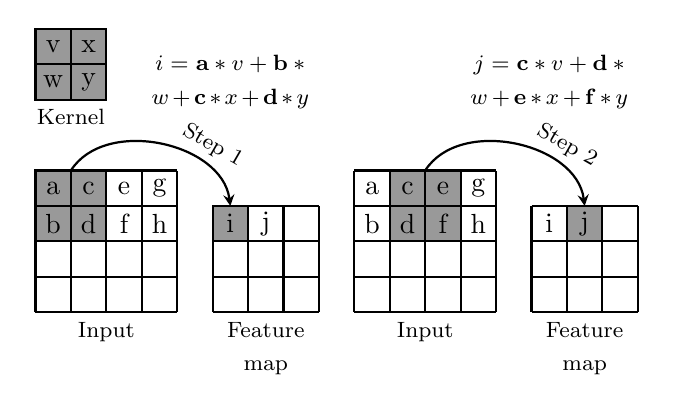
\begin{tikzpicture}
	%stride 1
	%kernel
	\draw [thick, draw=black, fill=black!40!white,scale = .45] (0,6) rectangle (2,8) grid (0,6);
	%kernel label
	\draw [scale=.45,below] node at (1,6)  {\footnotesize Kernel};
	%kernel components
	\draw [scale=.45] node at (0.5,7.5) {v};
	\draw [scale=.45] node at (0.5,6.5) {w};
	\draw [scale=.45] node at (1.5,7.5) {x};
	\draw [scale=.45] node at (1.5,6.5) {y};
	%step 1 equation
	\draw [scale=.45] node [text width=2cm,align=center] at (5.5,6.5) {\footnotesize \(i=\mathbf{a}*v+\mathbf{b}*w+\mathbf{c}*x+\mathbf{d}*y\)};
	%step 2 equation
	\draw [scale=.45] node [text width=2cm,align=center] at (14.5,6.5) {\footnotesize \(j=\mathbf{c}*v+\mathbf{d}*w+\mathbf{e}*x+\mathbf{f}*y\)};
	\draw [thick, draw=black, fill=black!40!white,scale = .45] (0,2) rectangle (2,4);
	\draw [thick, draw=black,scale=.45] (0,0) grid  (4,4) node at (2,0)[below] {\footnotesize Input};
	\draw [thick, draw=black, fill=black!40!white,scale = .45] (5,2) rectangle  (6,3);
	\draw [thick, draw=black,scale = .45] (5,0) grid  (8,3) node at (6.5,0) [below,text width=1.5cm,align= center] {\footnotesize Feature map};
	%
	\draw [thick, draw=black, fill=black!40!white,scale = .45] (10,2) rectangle  (12,4);
	\draw [thick, draw=black,scale = .45] (9,0) grid  (13,4) node at (11,0) [below] {\footnotesize Input};
	\draw [thick, draw=black, fill=black!40!white,scale = .45] (15,2) rectangle  (16,3);
	\draw [thick, draw=black,scale = .45] (14,0) grid  (17,3) node at (15.5,0) [below, text width=1.5cm,align=center] {\footnotesize Feature map};
	%draw arrows
	\draw [scale=.45,thick,arrow] (1,4)  to [bend angle=70, bend left] (5.5,3);
	\draw [scale=.45,thick,arrow] (11,4)  to [bend angle=70, bend left] (15.5,3);
	%draw step
	\draw [scale=.45] node[rotate=-30]   at (5,4.7) {\footnotesize Step 1};
	\draw [scale=.45] node[rotate=-30]   at (15,4.7) {\footnotesize Step 2};
	%draw abc step 1
	\draw [scale=.45] node at (0.5,3.5) {a};
	\draw [scale=.45] node at (1.5,3.5) {c};
	\draw [scale=.45] node at (0.5,2.5) {b};
	\draw [scale=.45] node at (1.5,2.5) {d};
	\draw [scale=.45] node at (2.5,3.5) {e};
	\draw [scale=.45] node at (2.5,2.5) {f};
	\draw [scale=.45] node at (3.5,3.5) {g};
	\draw [scale=.45] node at (3.5,2.5) {h};
	\draw [scale=.45] node at (5.5,2.5) {i};
	\draw [scale=.45] node at (6.5,2.5) {j};
	%draw abc step 2
	\draw [scale=.45] node at (9.5,3.5)  {a};
	\draw [scale=.45] node at (10.5,3.5) {c};
	\draw [scale=.45] node at (9.5,2.5)  {b};
	\draw [scale=.45] node at (10.5,2.5) {d};
	\draw [scale=.45] node at (11.5,3.5) {e};
	\draw [scale=.45] node at (11.5,2.5) {f};
	\draw [scale=.45] node at (12.5,3.5) {g};
	\draw [scale=.45] node at (12.5,2.5) {h};
	\draw [scale=.45] node at (14.5,2.5) {i};
	\draw [scale=.45] node at (15.5,2.5) {j};
\end{tikzpicture}
}}
				}
				\only<3>{\subfloat[Convolutional operation, 2 strided.]{
						\scalebox{.5}[.5]{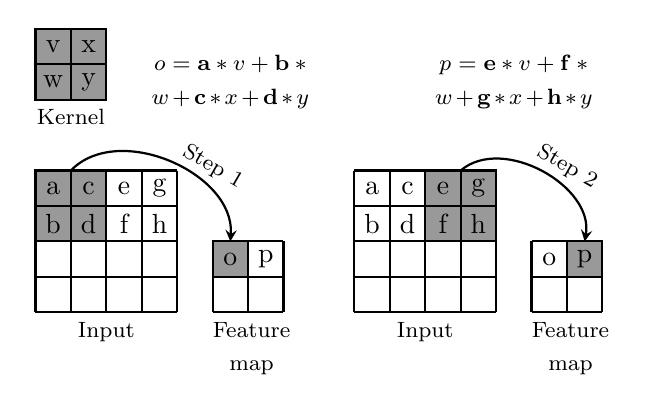
\begin{tikzpicture}
	%stride 2
	%kernel
	\draw [thick, draw=black, fill=black!40!white,scale = .45] (0,6) rectangle (2,8) grid (0,6);
	%kernel label
	\draw [scale=.45,below] node at (1,6)  {\footnotesize Kernel};
	%kernel components
	\draw [scale=.45] node at (0.5,7.5) {v};
	\draw [scale=.45] node at (0.5,6.5) {w};
	\draw [scale=.45] node at (1.5,7.5) {x};
	\draw [scale=.45] node at (1.5,6.5) {y};
	%step 1 equation
	\draw [scale=.45] node [text width=2cm,align=center] at (5.5,6.5) {\footnotesize \(o=\mathbf{a}*v+\mathbf{b}*w+\mathbf{c}*x+\mathbf{d}*y\)};
	%step 2 equation
	\draw [scale=.45] node [text width=2cm,align=center] at (13.5,6.5) {\footnotesize \(p=\mathbf{e}*v+\mathbf{f}*w+\mathbf{g}*x+\mathbf{h}*y\)};
	\draw [thick, draw=black, fill=black!40!white,scale = .45] (0,2) rectangle  (2,4);
	\draw [thick, draw=black,scale = .45] (0,0) grid  (4,4) node at (2,0)[below] {\footnotesize Input};;
	\draw [thick, draw=black, fill=black!40!white,scale = .45] (5,1) rectangle  (6,2);
	\draw [thick, draw=black,scale = .45] (5,0) grid  (7,2) node at (6.1,0) [below,text width=1.5cm,align= center] {\footnotesize Feature map};;
	%
	\draw [thick, draw=black, fill=black!40!white,scale = .45] (11,2) rectangle  (13,4);
	\draw [thick, draw=black,scale = .45] (9,0) grid  (13,4) node at (11,0) [below] {\footnotesize Input};;
	\draw [thick, draw=black, fill=black!40!white,scale = .45] (15,1) rectangle  (16,2);
	\draw [thick, draw=black,scale = .45] (14,0) grid  (16,2) node at (15.1,0) [below, text width=1.5cm,align=center] {\footnotesize Feature map};;
	%draw arrows
	\draw [scale=.45,thick,arrow] (1,4)  to [bend angle=70, bend left] (5.5,2);
	\draw [scale=.45,thick,arrow] (12,4)  to [bend angle=70, bend left] (15.5,2);
	%draw step
	\draw [scale=.45] node[rotate=-30]   at (5,4.1) {\footnotesize Step 1};
 	\draw [scale=.45] node[rotate=-30]   at (15,4.1) {\footnotesize Step 2};
	%draw abc step 1
	\draw [scale=.45] node at (0.5,3.5) {a};
	\draw [scale=.45] node at (1.5,3.5) {c};
	\draw [scale=.45] node at (0.5,2.5) {b};
	\draw [scale=.45] node at (1.5,2.5) {d};
	\draw [scale=.45] node at (2.5,3.5) {e};
	\draw [scale=.45] node at (2.5,2.5) {f};
	\draw [scale=.45] node at (3.5,3.5) {g};
	\draw [scale=.45] node at (3.5,2.5) {h};
	\draw [scale=.45] node at (5.5,1.5) {o};
	\draw [scale=.45] node at (6.5,1.5) {p};
	%draw abc step 2
	\draw [scale=.45] node at (9.5,3.5)  {a};
	\draw [scale=.45] node at (10.5,3.5) {c};
	\draw [scale=.45] node at (9.5,2.5)  {b};
	\draw [scale=.45] node at (10.5,2.5) {d};
	\draw [scale=.45] node at (11.5,3.5) {e};
	\draw [scale=.45] node at (11.5,2.5) {f};
	\draw [scale=.45] node at (12.5,3.5) {g};
	\draw [scale=.45] node at (12.5,2.5) {h};
	\draw [scale=.45] node at (14.5,1.5) {o};
	\draw [scale=.45] node at (15.5,1.5) {p};
\end{tikzpicture}}}
				}
				\only<4>{\subfloat[Even deconvolution]{
						\scalebox{.5}[.5]{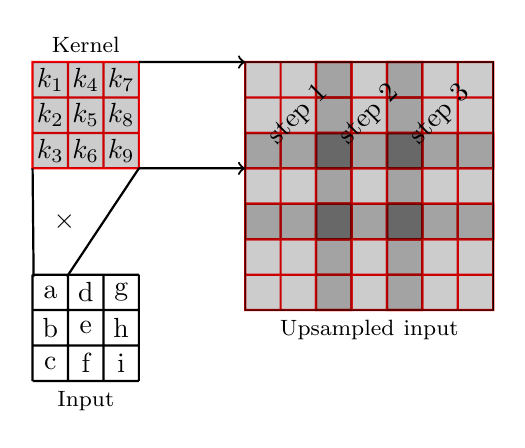
\begin{tikzpicture}

\begin{scope}[transparency group]
\begin{scope}[blend mode=multiply]
%stride 1
%kernel
\draw [thick, draw=red,fill=black!20!white, scale = .45] (-1,5) grid (2,8) rectangle (-1,5);
%kernel label
\draw [scale=.45,above] node at (0.5,8)  {\footnotesize Kernel};
%kernel components
\draw [scale=.45] node at (-0.5,7.5) {$k_1$};
\draw [scale=.45] node at (-0.5,6.5) {$k_2$};
\draw [scale=.45] node at (-0.5,5.5) {$k_3$};
\draw [scale=.45] node at (0.5,7.5)  {$k_4$};
\draw [scale=.45] node at (0.5,6.5)  {$k_5$};
\draw [scale=.45] node at (0.5,5.5)  {$k_6$};
\draw [scale=.45] node at (1.5,7.5)  {$k_7$};
\draw [scale=.45] node at (1.5,6.5)  {$k_8$};
\draw [scale=.45] node (k9) at (1.5,5.5)  {$k_9$};
%kernel on output
\draw [scale=.45] node[rotate=45] at (6.5,6.5)  {step 1};
\draw [scale=.45] node[rotate=45] at (8.5,6.5)  {step 2};
\draw [scale=.45] node[rotate=45] at (10.5,6.5)  {step 3};
%Kernel label
\draw [thick, draw=black,scale=.45] (-1,-1) grid  (2,2) node at (0.5,-1)[below] {\footnotesize Input};
% step 1 featuremap
\draw [thin, draw=black ,scale = .45] (5,1) rectangle  (12,8) node at (8.5,1) [below,text width=3cm,align= center] {\footnotesize Upsampled input};
%draw abc step 1
\draw [scale=.45] node (a) at (-.5,1.5) {a};
\draw [scale=.45] node at (-.5,0.5) {b};
\draw [scale=.45] node at (-.5,-.5) {c};
\draw [scale=.45] node at (0.5,1.5) {d};
\draw [scale=.45] node at (0.5,0.5) {e};
\draw [scale=.45] node at (0.5,-.5) {f};
\draw [scale=.45] node at (1.5,1.5) {g};
\draw [scale=.45] node at (1.5,0.5) {h};
\draw [scale=.45] node at (1.5,-.5) {i};
%draw connections
\draw [thick,scale=.45] (a.north east) -- (2,5) {};
\draw [thick,scale=.45] (a.north west) -- (-1,5){};
\draw [->,thick,scale=.45] (2,5) -- (5,5){};
\draw [->,thick,scale=.45] (2,8) -- (5,8){};
\draw [scale=.45,thick] node at (-.1,3.5) {$\mathbf{\times}$};
%draw kernel positions 
\foreach \i in {1,3,5}{
\foreach \j in {5,7,9}{
	\draw [thick, draw=red, fill=black!20!white,scale = .45] (\j,\i) grid  (\j+3,\i+3) rectangle (\j,\i);
		}
		}
\end{scope}
\end{scope}
\end{tikzpicture}
}}
				}
				\only<5->{\subfloat[Uneven deconvolution]{
						\scalebox{.5}[.5]{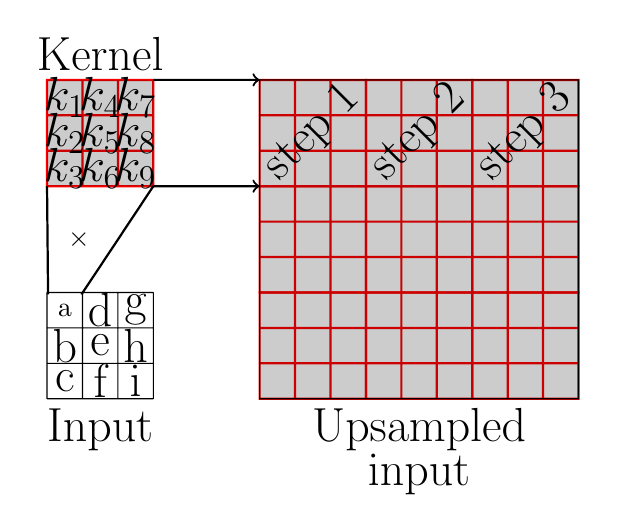
\begin{tikzpicture}
\begin{scope}[transparency group]
\begin{scope}[blend mode=multiply]

%kernel
\draw [thick, draw=red, fill=black!20!white,scale = .45] (-1,5) rectangle (2,8) grid (-1,5);
%kernel label
\draw [scale=.45,above] node at (0.5,8)  {\LARGE Kernel};
%kernel components
\draw [scale=.45] node at (-0.5,7.5) {\LARGE $k_1$};
\draw [scale=.45] node at (-0.5,6.5) {\LARGE $k_2$};
\draw [scale=.45] node at (-0.5,5.5) {\LARGE $k_3$};
\draw [scale=.45] node at (0.5,7.5)  {\LARGE $k_4$};
\draw [scale=.45] node at (0.5,6.5)  {\LARGE $k_5$};
\draw [scale=.45] node at (0.5,5.5)  {\LARGE $k_6$};
\draw [scale=.45] node at (1.5,7.5)  {\LARGE $k_7$};
\draw [scale=.45] node at (1.5,6.5)  {\LARGE $k_8$};
\draw [scale=.45] node (k9) at (1.5,5.5)  {\LARGE $k_9$};
%kernel on output
\draw [scale=.45] node [rotate=45] at (6.5,6.5)  {\LARGE step 1};
\draw [scale=.45] node [rotate=45] at (9.5,6.5)  {\LARGE step 2};
\draw [scale=.45] node [rotate=45] at (12.5,6.5) {\LARGE step 3};

% input label
\draw [thin, draw=black,scale=.45] (-1,-1) grid  (2,2) node at (0.5,-1)[below] {\LARGE Input};
% step 1 featuremap;
\draw [thin, draw=black,scale = .45] (5,-1) rectangle  (14,8) node at (9.5,-1) [below,text width=4cm,align= center] {\LARGE Upsampled input};
%draw abc
\draw [scale=.45] node (a) at (-.5,1.5) {a};
\draw [scale=.45] node at (-.5,0.5) {\LARGE b};
\draw [scale=.45] node at (-.5,-.5) {\LARGE c};
\draw [scale=.45] node at (0.5,1.5) {\LARGE d};
\draw [scale=.45] node at (0.5,0.5) {\LARGE e};
\draw [scale=.45] node at (0.5,-.5) {\LARGE f};
\draw [scale=.45] node at (1.5,1.5) {\LARGE g};
\draw [scale=.45] node at (1.5,0.5) {\LARGE h};
\draw [scale=.45] node at (1.5,-.5) {\LARGE i};
%draw connections
\draw [thick,scale=.45] (a.north east) -- (2,5) {};
\draw [thick,scale=.45] (a.north west) -- (-1,5){};
\draw [->,thick,scale=.45] (2,5) -- (5,5){};
\draw [->,thick,scale=.45] (2,8) -- (5,8){};
\draw [scale=.45,thick] node at (-.1,3.5) {$\mathbf{\times}$};
\foreach \i in {-1,2,5}
\foreach \j in {5,8,11}
	\draw [thick, draw=red, fill=black!20!white,scale = .45] (\j,\i) grid  (\j+3,\i+3) rectangle (\j,\i);

\end{scope}
\end{scope}
\end{tikzpicture}
}}
				}
				\caption{Fundamental features of conv. networks.}
			\end{figure}
		\end{column}
		\begin{column}{.5\textwidth}
			\begin{itemize}
				\item Designed for 2D/3D input
				\item<6->\emph{Peculiarities}: Sparse connections, parameter sharing
				\begin{itemize}
					\item<6->Promotes generalization
				\end{itemize}
				\item<7->\emph{Hyperparameters}: Number \& size of layers, kernel dimensions, stride increments
				\begin{itemize}
					\item<8->Non-trivial influence of output dimensions \& quality
				\end{itemize}  
			\end{itemize}
		\end{column}
	\end{columns}
\end{frame}
\end{document}
